\documentclass[a4paper, 10pt]{book}
%\newcommand\hmmax{0}
%\newcommand\bmmax{0}
\usepackage[T1]{fontenc}
\usepackage{amsmath}
%\usepackage{amsfonts}
\usepackage[margin=0.5in]{geometry}
\usepackage{amssymb}
\setlength{\parindent}{0pt}
\usepackage{amscd,amsthm,hyperref,mathrsfs,multirow,xcolor,lscape,ifthen,mathtools,graphicx,fancyhdr,enumerate,bbm}
\usepackage{fancyhdr}
\pagestyle{fancy}
\usepackage{calc}
\newlength{\pageoffset}
\setlength{\pageoffset}{0cm}% use whatever you like
\fancyheadoffset[L,R]{\pageoffset}
\fancyfootoffset[L, R]{\pageoffset}
\renewcommand{\chaptermark}[1]{\markboth{#1}{}}
\renewcommand{\sectionmark}[1]{\markright{#1}{}}
\fancyhf{}
\fancyhead[LE]{\scshape\thechapter\quad\leftmark}
\fancyhead[RO]{\scshape\thesection\quad\rightmark}
\fancyfoot[C]{\thepage}
 \renewcommand{\footrulewidth}{0.8pt}
 \renewcommand{\headrulewidth}{0.8pt}
\fancypagestyle{plain}{%
  \fancyhf{}%
  \fancyfoot[C]{\thepage}%
  \renewcommand{\headrulewidth}{0pt}% Line at the header invisible
  \renewcommand{\footrulewidth}{0.8pt}% Line at the footer visible
}
%\mathtoolsset{showonlyrefs=true}
\usepackage[thinlines]{easytable}
\usepackage[toc,page]{appendix}
\usepackage{hyperref}
\usepackage{stmaryrd}
\usepackage{cleveref}
\usepackage{mathtools}

%\usepackage[condensed,math]{kurier}
%\usepackage{newpxtext,newpxmath}
%\usepackage[garamond]{mathdesign}
\usepackage{xcolor}
\setcounter{tocdepth}{1}
\setcounter{secnumdepth}{1}   
\usepackage[DIV=13]{typearea}
\usepackage[all,cmtip]{xy}
\usepackage{tikz}
\usepackage{bbm}
\usepackage{braids}
\usepackage{tabu}
\usepackage{emptypage}
\usepackage{blindtext}
\usetikzlibrary{matrix}
\usetikzlibrary{calc}
\graphicspath{ {./pics/} }
\usepackage{listings}
\lstset{language=GAP,rangeprefix=\#\&\ ,rangesuffix=\ \#\&,includerangemarker=false, numbers=left,   inputencoding=latin1,
   basicstyle=\sffamily\footnotesize}

\usepackage{tikz-qtree}
\usetikzlibrary{matrix}
\usetikzlibrary{calc}
\newcommand{\red }[1]{{\color{red}#1}}
\newcommand{\blue}[1]{{\color{blue}#1}}
\newcommand{\green}[1]{{\color{green}#1}}
\newcommand{\brown}[1]{{\color{brown}#1}}
\newcommand{\purple}[1]{{\color{purple}#1}}
 \newtheorem{Thm}{Theorem}[chapter]
 \newtheorem{theorem}{Theorem}[chapter]
 \newtheorem{Lem}[theorem]{Lemma}
 \newtheorem{Prop}[theorem]{Proposition}
 \newtheorem{Cor}[theorem]{Corollary}
   \newtheorem{Claim}[theorem]{Claim}
 \newtheorem{Conj}[theorem]{Conjecture}
 \newtheorem{Expl}[theorem]{Example}
\newtheorem{Expls}[theorem]{Examples}
 \newtheorem{Rem}[theorem]{Remark}
\newtheorem{Qu}[theorem]{Question}
\theoremstyle{definition}
 \newtheorem{Def}[theorem]{Definition}
 \newtheorem{defn}[theorem]{Definition}
\numberwithin{equation}{chapter}
\newcommand\N{\mathbb N}
%\renewcommand\tagform@[1]{}
\newcommand\identify{\quad\hat{=}\quad}
\newcommand\ol[1]{\overline{#1}}
\newcommand{\tmt}[4]{\left({#1\atop #3}{#2\atop #4}\right)}
\newcommand\tr{\operatorname{tr}}
\newcommand\End{\operatorname{End}}
\newcommand\lstl{\lstinline}
\newcommand\ptr{\text{ptr}}
\newcommand\ac{\text{ac}}
\newcommand\hit{\triangleright}
\newcommand\tot{\varphi}
\newcommand\bhit{\blacktriangleright}
\newcommand\inv{^{-1}}
\def\HM#1.#2.#3.#4.{{^{#1}_{#3}\mathcal M^{#2}_{#4}}}
\newcommand\lYD[1]{{^{#1}_{#1}\mathcal{YD}}}

\newcommand\id{\operatorname{id}}
\newcommand{\ie}{i.e.,}
\newcommand\ot{\otimes}
\newcommand{\ou}[1]{\underset{{#1}}{\otimes}}
\newcommand{\co}[1]{\mathrel{\mathop{\Box}_{#1}}}
\newcommand\Ob{\textnormal{Ob }}
\newcommand\Res{\operatorname{Res}}
\newcommand\Ind{\operatorname{Ind}}
\newcommand\Coind{\operatorname{Coind}}
\newcommand\Stab{\operatorname{Stab}}
\newcommand\Rep{\operatorname{Rep}}
\newcommand\Irr{\operatorname{Irr}}
\newcommand\Vect{\operatorname{Vec}}
\newcommand\Tr{\operatorname{Tr}}
\newcommand\lquot{\backslash}
\newcommand\Img{\operatorname{im}}
\newcommand\Mor{\operatorname{Mor}}
\newcommand\Bimod{\operatorname{Bimod}}
\newcommand\Fun{\operatorname{Fun}}
\newcommand\Hom{\operatorname{Hom}}
\newcommand\Aut{\operatorname{Aut}}
\newcommand\Ext{\operatorname{Ext}}
\newcommand\Mod{\operatorname{Mod}}
\newcommand\Forg{\operatorname{Forg}}
\newcommand\GL{\operatorname{GL}}
\newcommand\Indtobim{\mathcal F}
\newcommand\IndtoYD{\mathcal G}
\newcommand\FPdim{\text{FPdim}}
\newcommand\Q{\mathbb Q}
\newcommand\CC{\mathbb C}
\newcommand\ZZ{\mathbb Z}
\newcommand\R{\mathbb R}
\newcommand\kk{\mathbb C}
\newcommand\CCu{\CC^\times}
\newcommand\op{^{\text{op}}}
\newcommand\Z{\mathbb Z}
\newcommand\M{\mathcal{M}}
\newcommand\NN{\mathcal{N}}
\newcommand\C{\mathcal C}
\newcommand\Cat{\mathcal C}
\newcommand\OO{\mathcal O}
\newcommand\D{\mathcal D}
\newcommand\A{\mathcal A}
\newcommand\B{\mathcal B}
\newcommand\CTR{\mathcal Z}
\newcommand \I{\mathcal I }
\newcommand\galaut{\sigma}
\newcommand{\ra}\rightarrow
\newcommand{\xra}\xrightarrow
\newcommand\adams{\psi}
\newcommand\auta{\psi}
\newcommand\autb{\widetilde\psi}
\newcommand\doubleadams{\widehat\psi}
\newcommand\wreath{\wr}
\newcommand\semdir{\rtimes}
\newcommand\one{\mathbf{1}}
\newcommand\semidir\rtimes
\newcommand\coeff{C(a,b)}
\newcommand\ev{\operatorname{ev}}
\newcommand\coev{\operatorname{coev}}
\newcommand\Inf{\operatorname{Inf}}
\newcommand\Gal{\operatorname{Gal}}
\newcommand\ab{{\operatorname{ab}}}
\newcommand{\gb}{\overline{g}}
\newcommand{\hb}{\overline{h}}
\newcommand{\kb}{\overline{k}}
\newcommand{\pb}{\bar{p}}
\newcommand{\qb}{q_a}
\newcommand{\nb}{\bar{n}}
\newcommand{\pt}{\tilde{p}}
\newcommand{\nt}{m}
\newcommand{\qt}{\tilde{q}}

\makeatletter
\newcommand\ackname{Acknowledgements}
\if@titlepage
   \newenvironment{acknowledgements}{%
       \titlepage
       \null\vfil
       \@beginparpenalty\@lowpenalty
       \begin{center}%
         \bfseries \ackname
         \@endparpenalty\@M
       \end{center}}%
      {\par\vfil\null\endtitlepage}
\else
   \newenvironment{acknowledgements}{%
       \if@twocolumn
         \section*{\abstractname}%
       \else
         \small
         \begin{center}%
           {\bfseries \ackname\vspace{-.5em}\vspace{\z@}}%
         \end{center}%
         \quotation
       \fi}
       {\if@twocolumn\else\endquotation\fi}
\fi
\makeatother

\newenvironment{abstract}{}{}
\usepackage{abstract}
\title{Algebraic and topological invariants of fusion categories}
\author{Ajinkya Kulkarni}
\usepackage{libertine}
\usepackage{libertinust1math}

\begin{document}

%\renewcommand{\theequation}{\arabic{chapter}.\arabic{section}.\arabic{equation}}

\maketitle

\begin{acknowledgements}

\thispagestyle{plain}
This thesis owes its existence majorly to the friendly guidance and generous support of my advisor, Peter Schauenburg, from whom I have learnt not only a lot of mathematics but also how to express it well (I hope). I'd like to thank him for patiently answering my questions and also for fetching the burgers on most Wednesdays.\\
I would like to thank Jitendra Bajpai for introducing me to the number-theoretic aspects of modular fusion categories, Ehud Meir for introducing me to a lot of new and exciting mathematics and for help with some of the proofs in chapter \ref{prelims} and Michael Mignard for his help with the code and for collaboration on \cite{kulkarni2018topological}. Thanks to Kenji Iohara and Victor Ostrik and Ingo Runkel for helpful conversations and to Graham Ellis for help with GAP. \\
I am thankul to the \'Ecole-Doctorale Carnot-Pasteur and the IMB for funding some of my travel to conferences. \\
Thanks to Raveena Palli for help with drawing the string diagrams. I'd also like to acknowledge Rohit Gupta for his constant encouragement.  Lastly, I thank my family and friends for their support.
\end{acknowledgements}

  \clearpage
\begin{center}
    \thispagestyle{empty}
    \vspace*{\fill}
    \textit{To my late grandmothers, Shalini Kulkarni and Malti Dhavs\'e}
    \vspace*{\fill}
\end{center}
\clearpage
\tableofcontents

\chapter{Introduction}\label{intro}
\pagenumbering{arabic}
Fusion categories arise as the right categorical setting to think about the representation theory of various kinds of algebraic objects (finite groups, semisimple Hopf algebras, loop groups, affine Lie algebras, etc.). They are of interest not only from a representation-theoretic perspective but also due to their links with topological field theory \cite{T, MR3644796}, operator algebras \cite{MR3367967} and quantum computing \cite{MR2640343}. \\
Fusion categories may be equipped with a \textit{ribbon} structure, and when this ribbon structure satisfies certain conditions, we get what are called \textit{modular} fusion categories. The adjective `modular' is attributed to the fact that MFCs give rise to a projective representation of the modular group $\text{PSL}_2(\Z)$, which is comprised of the $S$-matrix and the $T$-matrix.
On the one hand one could say that these two matrices are just particular instances of the topological invariants defined by a GTCs in the framework of a topological quantum field theory: the $S$-matrix is the invariant defined for a Hopf link colored by two simples of the category, and the $T$-matrix contains the components of a kink. On the other hand, one may feel that the modular data is somewhat privileged among the topological invariants associated to the category: Invertibility of the $S$-matrix already features in the definition; invariance properties with respect to the modular group are key for the appearance of modular categories in conformal field theory; last but not least properties of the modular data are important for the purely algebraic study of modular categories. The importance of the modular data has led to the question being seriously considered (and stated as not quite a conjecture in \cite{MR3486174}) as to whether a modular category (and hence the TQFT associated to it) is already determined fully by the modular data. This was refuted in \cite{2017arXiv170802796M} by a family of examples that are taken among the particularly accessible class of group-theoretical modular categories, more specifically the Drinfeld centers of pointed fusion categories, which were already considered, in the guise of representation categories of twisted Drinfeld doubles of finite groups, in \cite{DijPasRoc:QHAGCOM}. It turns out in fact that arbitrarily many inequivalent modular categories can give rise to the same modular data; the examples are defined by the same noncommutative group, endowed with different three-cocycles; the smallest example in \cite{2017arXiv170802796M} concerns the nonabelian group of order $55$, although it is not known whether smaller examples exist.\\
In Chapter 3, we introduce a topological invariant arising from an MFC (one among the infinitely many invariants furnished by the TQFT associated with the MFC) which we call the Borromean tensor (or the $B$-tensor), in the hope that it would be able to "see" some data about the MFC that the modular data does not. The $B$-tensor is partly an obvious candidate for naive reasons: It is the closure of a three-strand braid, which is the next more complicated thing over the two-strand braid whose closure is the Hopf link; having three strands might allow the associativity constraint of the category (which, after all, is encoded in the three-cocycle that makes the basic difference in the aforementioned examples)  to have a greater influence on the invariant. Since the invariant obtained from a full twist on three strands (like the Hopf link comes from a full twist on two strands) can be determined by the modular data, making inverse braidings appear seems necessary, and the braid whose closure gives the borromean rings does this in a somewhat symmetric fashion. It may also be a good candidate for a slightly less naive reason: The borromean rings are three circles that are pairwise not linked, yet form a nontrivial link.\\
\begin{figure}[h!]
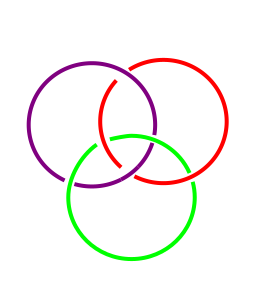
\includegraphics[width=0.3\textwidth]{b-tensorc.eps}
\centering
\caption{The borromean rings}
\end{figure}\\
While the objective of defining the $B$-tensor was to distinguish twisted Drinfeld doubles of nonabelian groups of order $pq$ where $p,q$ are prime and $p|q-1$, which it did successfully in conjunction with the $T$-matrix, it turns out that the $B$-tensor and the $T$-matrix are sufficient to distinguish a larger class of twisted Drinfeld doubles, namely those coming from square free groups (i.e., groups whose order has no repeated prime factor).
\begin{Thm}[=Theorem \ref{thm:BT}]
 The $B$-tensor and the $T$-matrix together completely distinguish Drinfeld centers of pointed fusion categories $\CTR(\Vect^\omega_G)$, where $G$ is a square-free group.
 \end{Thm} 
We also prove a small theorem about modular data-preserving bijections between twisted doubles of non-isomorphic square-free groups belonging to the same \textit{Art} (see section \ref{sub:twisted_doubles_of_square-free groups} for this terminology). This part of the thesis is based on two joint papers, one with M. Mignard and P. Schauenburg (for the $pq$ case) and another with P. Schauenburg (for the square free case).\\\\
The second part of this thesis concerns group theoretical fusion categories (henceforth called group theoretical categories or GTCs), of which pointed fusion categories as well as their Drinfeld centers are a special case. GTCs  have been of interest since they were introduced in \cite{Ost:MCDDFG}, as they provide concrete, non-trivial examples of fusion categories in terms of rather elementary algebraic and cohomological data, i.e., such a category may be constructed starting from the 4-tuple $(G, H, \omega, \mu)$ where $G$ is a finite group, $H$ a subgroup of $G$, $\omega$ a 3-cocycle on $G$ and $\mu$ a 2-cochain on $H$ such that $\omega|_{H\times H\times H} = d\mu$. More conceptually, every GTC $\C(G, H, \omega, \mu)$ arises as the category of $\Vect^\omega_G$-module endofunctors of $\Mod_{\Vect^\omega_G}(\kk_\mu H)$, which is the category of modules over an indecomposable algebra object $\CC_\mu H$ (the group algebra of $H$ with multiplication is twisted by $\mu$) in $\Vect^\omega_G$. Thanks to a theorem of Ostrik (see Theorem \ref{Ostrik}), every such GTC is Morita equivalent to $\Vect^\omega_G$ by construction. As a fusion category, the Drinfeld center of $\Vect^\omega_G$ can be described as $\C(G\times G, \Delta(G\times G), \omega, 1)$, where $\Delta$ denotes the diagonal subgroup. For numerous known examples of finite-dimensional semisimple Hopf algebras $H$ over $\CC$, $\Rep(H)$ is group theoretical, and it was a widely believed conjecture that this is true for any such $H$ until Nikshych \cite{MR2480712} constructed a class of counterexamples. GTCs have been studied in some detail, see \cite{MR2710113}, \cite{MR2559854}. The recent work of Morales et al. \cite{2020arXiv200103837M} gives a classification of indecomposable algebra objects in GTCs. S. Natale computed Frobenius-Schur indicators for GTCs in \cite{Nat:FSICFC}. Much earlier, similar constructions to the ones used in this part of the thesis have been considered in \cite{MR1887584}, and later by \cite{Zhu:HARRHA} for applications to Hecke algebras.\\
The fusion ring of a fusion category is an important invariant, in that in conjunction with the associators for every triple of objects, it provides a complete description of the fusion category in question. An important question concerning fusion rings is: how many fusion categories may be constructed from a given fusion ring? In the case of rank 2 for example, Ostrik provides a complete answer to this question in \cite{O}. Classifications of fusion categories (with extra structure and/or conditions) coming from fusion rings of higher ranks are also available in the literature \cite{MR2422269,MR3427429}. However, our attempts are in a rather different (or perhaps even opposite) and more humble direction, in the sense that we only look at fusion rings coming from the rather specialized (albeit accessible) class of GTCs $\C(G, H, \omega, \mu)$. In particular, we provide an algorithm that can determine the fusion rules of a GTC starting from group theoretical data. Until now, there was no known algorithmic way to compute fusion rules for general GTCs (except for twisted doubles, where one simply uses the Verlinde formula). In the case where $\omega$ and $\mu$ are trivial, (i.e., the group theoretical data is of the form $(G, H, 1, 1)$) there is a geometric description of the fusion rules given in \cite{MR1444783}. A generalization of this geometric approach to the general case is an interesting prospect certainly worth exploring.\\
However, we use a more explicit algebraic approach to the problem. Firstly, our work is simplified by the observation that any GTC $\C(G, H, \omega, \mu)$ is equivalent to a GTC of the form $\C(G, H, \omega', 1)$ where $\omega'$ is an adapted cocycle, i.e., $\omega|_{G\times G \times H}= 1$. There is a well-known parametrization of the simple objects in a GTC $\C(G, H, \omega, 1)$, in terms of the data $(g, \eta)$ where $g\in G$ is a double $H$-coset representative, and $\eta$ is a character of $S_g:= \Stab_H(gH)$, the stabilizer of the coset $gH$ in $H$ (see \ref{simples}). We define a character theory for objects in $\C(G, H, \omega, 1)$, i.e., for an object $M\in \C(G, H, \omega, 1)$ one can define a character $\chi_M:G\times G\ra \kk$. This character behaves in a rather nice manner with respect to the tensor product $\otimes_H$ and also admits a suitably-defined inner product. In particular, we can define the character on a tensor product of object $M\ot_H N$, $\chi_{M\ot_H N}$ in terms of a suitable product of the characters $\chi_M$ and $\chi_N$. 
\begin{Thm}[=Theorem \ref{thm:tensorchar}]
For two objects $M, N \in \C(G, H, \omega, 1)$, the character $\chi_{M\ot N}$ can be expressed in terms of the characters $\chi_M$ and $\chi_N$ as  
\begin{equation*}
	\chi_{M\otimes_H N }(g,s) = \sum_{a\in Q} \omega(a, a\inv \hit s, a\inv g)\omega\inv(s,a, a\inv g) \chi_{M}(a,s)\chi_{N}(a\inv g, a\inv \hit s ),
\end{equation*} for $g, s\in G$, where $Q$ is a set of right $H$-coset representatives in $G$.
\end{Thm}
An inner product is defined analogous to  (but not quite the same as) that in the character theory of finite groups, and this completes the theoretical setup for calculating the fusion ring of $\C(G, H, \omega, 1)$. We compute fusion rings for group theoretical data where $|G|\leq 20$ and we make the following observations.  
\begin{Thm} [see section \ref{results}]
There are 34 distinct non-pointed fusion rings coming from group theoretical data with $|G|\leq 20$. Among these, there are 26 singly generated fusion rings. There are only 3 non-hyperrings, all of which are singly generated.
\end{Thm}

Studying the Frobenius-Schur indicators and Morita equivalence of GTCs using code from \cite{2017arXiv170806538M} provides several counter-examples to the following conjecture of Tucker \cite[Conjecture 5.6]{MR4044867}.
\begin{Conj}
Two Morita equivalent group theoretical fusion categories with $|G|\leq 20$ sharing the same fusion ring cannot be distinguished by their Frobenius-Schur indicators.
\end{Conj}
We obtain 7 sets of group-theoretical data, each one corresponding to GTCs that have the same fusion ring and are Morita equivalent but are distinguished by their Frobenius-Schur indicators. Among these, one set of data corresponds to a pointed fusion ring of rank 16, whereas the others correspond to fusion rings of rank 10 that are direct or semidirect products (as fusion rings) of a Tambara-Yamagami fusion ring with $C_2$. We provide more details in Section \ref{results}. This part of the thesis is joint work with P. Schauenburg.



\chapter{Preliminaries}\label{prelims}


This chapter covers some material necessary to understand the rest of this thesis. We define fusion categories and set up preliminary results that will be used later on. Almost all of the material in this chapter can be found (in a more general setting) somewhere in \cite{EGNO}.
\begin{Def}
An abelian category  is $\kk$-\textit{linear} if every set of morphisms is a  $\kk$-vector space and \textit{locally finite} if these vector spaces are all finite dimensional.
\end{Def}

\begin{Def}
An object $X$ in an abelian category is \textit{projective} if for any epimorphism $f:Y\ra Z$, and a morphism $h: X\ra Z$, there is a morphism $g: X\ra Y$, such that the following diagram commutes.
\[
\xymatrix{
	X \ar[rd]^h\ar@{-->}[d]_g\\
	Y \ar@{>>}[r]_f& Z
}
\] 
\end{Def}
\begin{Def}
A $\kk$-linear abelian category $\C$ is \textit{semisimple} if every object is projective. An object $X$ is \textit{simple} if $\C(X, X) = \kk$.
\end{Def}

Note that any object in a semisimple category can be written as a direct sum of finitely many simple objects, and this is an equivalent characterization of semisimplicity. Throughout this thesis, whenever a $\kk$-linear semisimple category $\C$ has a finite number of isomorphism classes of simple objects, we will denote by $\OO(\C)$ a chosen set of representatives of the isomorphism classes of simple objects. We may also abuse language and refer to the elements of $\OO(\C)$ as the simple objects of $\C$, this should not lead to any ambiguity.

\iffalse
\begin{Lem}
Let $F:\C \leftrightarrows \D: U$ be an adjunction between abelian categories. Then the right adjoint $U$ is faithful if and only if the counit $FU(X)\rightarrow X$ is a surjection for every object $X \in \D$. If in addition $U$ is exact then $U$ reflects isomorphisms.
\end{Lem}
\begin{proof}
Suppose $U$ is faithful, then by definition if $U(f) = 0$ for some morphism $f$ in $\D$, then $f=0$. Let $C$ be the cokernel of the counit map, $f: X \rightarrow C$, for some object $X\in \D$, then $f\circ \epsilon_X = 0$, consequently $U(f)\circ U(\epsilon_X) = 0$.  But the map $U(\epsilon_X)$ has a splitting given by the unit of the adjunction $\eta_{U(X)}$, so it is a surjection, and hence $U(f)=0$. Since $U$ is assumed faithful $f=0$, and so the counit has no cokernel, i.e., it is surjective. \\
Suppose the counit is surjective. Let $f:X\rightarrow Y$ be a morphism such that $U(f)=0$. Then by the naturality of the counit \begin{equation*}
	\xymatrix{
	FU(X) \ar[d]_{FU(f)} \ar[r]^{\epsilon_X} & X \ar[d]^{f} \\
	FU(Y) \ar[r]^{\epsilon_Y} & Y
	}
\end{equation*}                                                                                                             We get \begin{equation*}
	f\circ \epsilon_X = \epsilon_Y \circ FU(f) = 0,
\end{equation*}                                
and since $\epsilon_X$ is a surjection, $f=0$. Hence, $U$ is faithful.        
\end{proof}

\begin{Lem}
Let $F:\C \leftrightarrows  \D : U$ be an adjunction between $\kk$-linear categories in which $U$ and $F$ are $\kk$-linear functors, and $U$ is faithful and exact. If $\C$ is finite, then $\D$ is also finite.
\end{Lem}
\begin{proof}
To prove that $D$ is finite, we need to show (1) the morphism spaces are finite dimensional, (2) there are finitely many isomorphism classes of simple objects, (3) there are enough projectives, (4) every object has finite length.
To show (1), note that $U$ is faithful, \begin{equation*}
	\D(X, Y) \subseteq \C(U(X), U(Y))
\end{equation*} for every $X,Y \in \D$ so all morphism spaces in $\D$ are finite dimensional. To show (4), the fact that $U$ is a right adjoint means $U$ preserves products, so in particular, it preserves subobjects, and hence chains of subobjects. As $U$ reflects isomorphisms, it preserves strictly decreasing chains of subobjects. Since every object in $\C$ has finite length, so does every object in $\D$. For (3), let $P \twoheadrightarrow U(X)$, be a surjection for $X\in \D$, where $P$ is a projective object. $F$ being a left adjoint, it preserves surjections, and since we have shown that the counit of the adjunction is a surjection, the composite \begin{equation*}
	F(P) \rightarrow FU(X)\rightarrow X
\end{equation*}
is a surjection. The functor $\C(P, -)$ is exact, and since \begin{equation*}
	\C(P, U(-)) \cong \D(F(P), -), 
\end{equation*}
$\D(F(P), -)$ is exact, so $F(P)$ is projective. Finally, we need to show (2). For an object $X\neq 0 \in \D$, $U(X)\neq 0$ as U reflects isomorphisms. There is atleast one simple object $S$ such that $f:S\rightarrow U(X)$ is an injection. There is a unique map $\bar{f}:F(S) \rightarrow X$ such that $f = U(\bar{f})\circ\eta_S: S\rightarrow UF(S) \rightarrow U(X)$. If we consider the object $W= \bigoplus_{i\in \I} S_i$, $ S_i\in \OO(\C)$, then there exists a morphism $F(W) \rightarrow X$, for every $X\in \D$, which is a surjection if $X$ is simple. This means every simple object occurs as a simple factor in the composition series of $F(W)$. Since $F(W)$ is of finite length, and its composition series is unique upto isomorphism and permutation of factors (by the Jordan-H\"older theorem), there are finitely many isomorphism classes of simple objects in $\D$.      
\end{proof}
We are now ready to prove Proposition \ref{klinearfiniteness}. For a finite dimensional algebra $A$, the adjunction $F:\Vect \rightarrow A-\Mod: U$, where $F(X) = A\otimes X$ for $X\in \Vect$ and $U$ is the forgetful functor, satisfies the conditions necessary for the last lemma, so $A-\Mod$ is finite.


Let $\C$ be a finite $\kk$-linear category, For every $X_i\in \OO(\C)$ , pick a surjection $P_i\rightarrow X_i$,  with $P_i$ projective, and consider the finite dimensional vector space $A:=\C(P, P)$ where $P= \bigoplus P_i$. $A$ is a finite dimensional algebra, with multiplication given by $a\cdot b = b\circ a$.


We have the following adjunction \begin{equation*}
P\otimes_A -:	A-\Mod \leftrightarrows \C : A\otimes - : \C(P, -)
\end{equation*}
where the $A$-linear tensor product is defined as the coequalizer  \begin{equation*}
	P \otimes A \otimes - \rightrightarrows P\otimes -\rightarrow P\otimes_A -.
\end{equation*}
We only need to show that this adjunction is an equivalence; to do so we shall show that unit and counit of the adjunction are isomorphisms.
By definition of an adjunction, for an object $X\in A-\Mod$, \begin{align}
	\C(P\otimes_A X, P) &\cong \Hom _{A} (X, \C(P, P))\\
	\C(P \otimes_A X, P) &\cong \Hom_{A}(X, A) \\
	\C(P \otimes_A X, P) &\cong X
\end{align}
We have the unit of the adjunction $X\rightarrow \C(P \otimes_A X, P)$, and the computation above shows it is an isomorphism.
\fi 
\begin{Def}\rm
The \textit{Deligne tensor product} of two $\kk$-linear abelian categories $\C$ and $\D$, denoted $\C \boxtimes \D$, is an abelian category which is universal for the functor 
\newcommand{\Rex}{\text{Rex}}
\begin{equation}
	\label{deligne}F: \A \ra \Rex(\C \times \D, \A),
\end{equation} where $\A$ is a $\kk$-linear abelian category and $\Rex$ is the category of bilinear bifunctors which are right exact in both variables. In other words, there is a bilinear bifunctor $\boxtimes$, such that for any functor $F$ as in \eqref{deligne}, there is a unique right exact functor $\tilde{F}:\C\boxtimes \D\ra \A$ which satisfies $ F= \tilde{F}\circ \boxtimes$.
\end{Def}
Objects of $\C \boxtimes \D$ are of the form $X\boxtimes Y$ for objects $X\in \C$ and $Y\in \D$, whereas morphisms are of the form $f\boxtimes g: X\boxtimes Y \ra X' \boxtimes Y'$ for $f\in \C(X, X')$  and $g: \D(Y, Y')$. In the case where $\C$ and $\D$ are semisimple categories, the simple objects of $\C\boxtimes \D$ are of the form $X\boxtimes Y$, where $X\in \OO(\C)$ and $Y\in \OO(\D)$.
\begin{Rem}\rm
The Deligne tensor product is unique upto a unique equivalence.
\end{Rem}
\section{Tensor categories}
\begin{Def}
A \textit{monoidal category} is a category $\C$ is the data of a bifunctor $\C \times \C\rightarrow \C $, a natural isomorphism $a: \otimes \circ( \otimes \times \id) \rightarrow \otimes (\id \times \otimes)$ and a distinguished object $\one$, with natural isomorphism $l: \one\ot \id \rightarrow \id$ and $r:\id \ot \one \rightarrow \id$ such that the usual hexagon and triangle diagrams commute for any objects $W, X, Y, Z$ in $\mathcal{C}$.
\end{Def}
\begin{equation}\label{pentagon}
\xymatrix{
  	((W\otimes X)\otimes Y)\otimes  Z\ar[dd]_{a_{W\otimes X,Y,Z}}\ar[rr]^{a_{W,X,Y}} && (W\otimes(X\otimes Y))\otimes Z\ar[dr]^{a_{W,Y			\otimes Y,Z}}\\
   	& & & W\otimes((X\otimes Y)\otimes Z)\ar[dl]^{a_{X,Y,Z}}\\
  	(W\otimes X)\otimes(Y\otimes Z)\ar[rr]^{a_{W,X,Y\otimes Z}} && W\otimes(X\otimes (Y\otimes Z)))
 	}
\end{equation}

\begin{equation*}
\xymatrix{
(X \otimes \one) \otimes Y \ar[rr]^{a_{X,\textbf{1},Y}} \ar[dr]_{r_X \otimes \id_Y} && X \otimes(\one \otimes Y)\ar[dl]^{\id_X \otimes l_Y} \\ 
& X\otimes Y .
}
\end{equation*} 
A monoidal category where the functorial isomorphisms $a, l$ and $r$ are identities is called a strict monoidal category.
\begin{Def}
A \textit{monoidal functor} $F:(\C, \ot, \one)\rightarrow (\D, \otimes', \one')$ is a functor $F$ along with functorial isomorphisms \begin{align}
	J_{X, Y}: F(X) \otimes F(Y) &\rightarrow F(X\otimes Y)
	\end{align}
	and an isomorphism
	\begin{align}
	J_1: F(\one) &\cong \one'.
\end{align} 
for $ X, Y$ in $\C$ such that the associators of $\C$ and $\D$ are compatible with these isomorphisms, in the following way.
\[
\xymatrix{
(F(X)\ot F(Y)) \ot F(Z) \ar[rr]^{J_{X, Y}\otimes \id_{F(Z)}} \ar[d]^{\alpha_{F(X), F(Y), F(Z)}} & & F(X\ot Y)\ot F(Z) \ar[d]^{J_{X\otimes Y, Z}} \\
F(X)\ot (F(Y)\ot F(Z))\ar[d]^{\id_{F(X)}\ot J_{Y, Z}}	& & F((X\ot Y)\ot Z)\ar[d]^{F(\alpha_{X, Y, Z})} \\
F(X)\ot (F(Y\ot Z))  \ar[rr]^{J_{F(X), F(Y\otimes Z)}}& & F(X\ot (Y\ot Z))\\
}
\]

\end{Def}
 \begin{Def}
 A \textit{monoidal functorial isomorphism} is a functorial isomorphism between monoidal functors $\eta: F \ra G$ such that \[
\xymatrix { F(X)\ot F(Y) \ar[d]^{J_{X, Y}}\ar[r]^{\eta_X\ot\eta_Y} & G(X) \ot G(Y)\ar[d]^{J'_{X, Y}}\\
F(X\ot Y) \ar[r]^{\eta_{X\ot Y}} & G(X\ot Y),}
 \]
 where $J, J'$ are the accompanying functorial morphisms for $F, G$ respectively.
 \end{Def}
A monoidal functor whose isomorphisms $J$ and $J_1$ are identities is called a \textit{strict} monoidal functor.
\begin{Rem}\rm
We will often refer to $\kk$-linear abelian monoidal categories as \textit{tensor categories}. For tensor categories, the $\otimes$ functor is assumed to be bilinear and biadditive. Further, $\kk$-linear exact monoidal functors will often be called \textit{tensor functors}.
\end{Rem}

\begin{Rem}\rm
If $\C$ and $\D$ are tensor categories, then the Deligne tensor product $\C\boxtimes\D$ is also a tensor category, for details see \cite[Section 4.6]{EGNO}.
\end{Rem}
For a semisimple monoidal category $\C$ such that $\OO(\C)$ is finite, we can decompose the tensor product of two elements of $\OO(\C)$ as 
\begin{equation*}
	X \otimes Y \cong \bigoplus_{Z\in \OO (\C) } N^Z_{XY} Z 
\end{equation*} where $X, Y, Z \in \OO(\C)$. The non-negative integer $N^Z_{XY}$  is called the \textit{multiplicity} of $Z$ in $X\ot Y$. 
In case $\C$ is also $\kk$-linear structure and locally finite, the multiplicity can be expressed as, \begin{equation*}
	N^A_{BC} = \dim \C(A, B\ot C)
\end{equation*} for objects $A, B, C \in \C$.
\begin{Def}
For a semisimple monoidal category $\C$ such that $\OO(\C)$ is finite, there is a unique homomorphism called the Frobenius-Perron dimension \begin{equation*}
	\FPdim: \OO(\C) \rightarrow \R
\end{equation*}  
defined by $X\rightarrow \lambda_X$, where $\lambda$ denotes the largest non-negative real eigenvalue of the matrix $M$ which has all non-negative entries. These entries $M^Z_{Y}$ are defined by \begin{equation}\label{fusionrule}
	X \otimes Y \cong \bigoplus_{Z\in \OO (\C) } M^Z_{Y} Z 
\end{equation} 
where $Y \in \OO(\C)$. We will sometimes call $M$ the \textit{fusion matrix} of $X$.
\end{Def} Such an eigenvalue is guaranteed to exist for a matrix with non-negative integer entries by the Frobenius-Perron theorem, a proof of which is given in \cite[Theorem 3.2.1]{EGNO}.\\

\subsubsection{Graphical calculus}\label{graphicalcalculus}
Mac Lane's strictness theorem allows us to freely assume strictness for monoidal categories, which permits the use of the graphical calculus. We read diagrams top-to-bottom (the category theorists' convention) rather than bottom-to-top (the low-dimensional topologists' convention).
A morphism $f:X_1\ot\dots\ot X_n\ra Y_1\ot\dots\ot Y_m$ is represented as follows.
\begin{center}
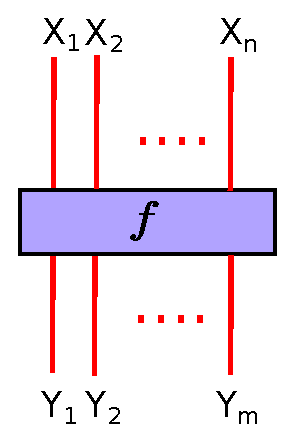
\includegraphics[width=0.15\textwidth]{morphnew.eps}
\end{center}
We will omit a strand if it is labelled by the unit object $\one$.
For morphisms $f:X\ra Y$, $g:Y\ra Z$, their composition $f\circ g: X\ra Z$ is denoted by stacking them.

\begin{center}
\includegraphics[width=0.04\textwidth]{morphism.eps}
\end{center}

For morphisms $f:X\ra Y, g:X'\ra Y'$, their tensor product $f\ot g: X\ot X' \ra Y \ot Y'$ is denoted as
\begin{center}
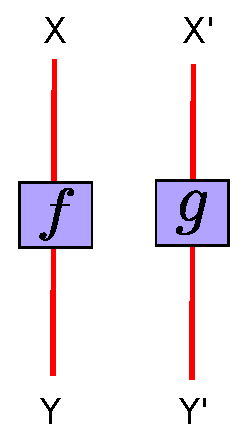
\includegraphics[width=0.1\textwidth]{tensor.eps}
\end{center}
The above rules easily generalize to cases when the source and/or target of a morphism consists of several tensor factors.
\subsection{Rigidity}
\begin{Def}
 A \textit{left rigid} structure on a strict monoidal category $\C$ is an endofunctor $*:\C \rightarrow \C, X\mapsto X^*$, with evaluation and coevaluation morphisms \begin{align}
	\coev: \one \rightarrow X\otimes X^*\quad, \quad \quad \ev:X^*\otimes X \rightarrow \one  
	,
\end{align}
depicted respectively as 
\begin{center}
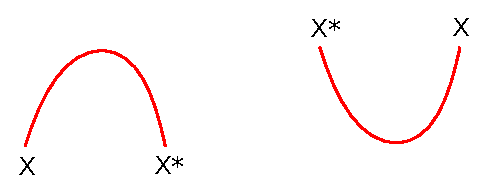
\includegraphics[width=0.4\textwidth]{duals.eps}
\end{center}
for each $X \in \C$ such that the following `snake diagrams' are satisfied,

\begin{center}
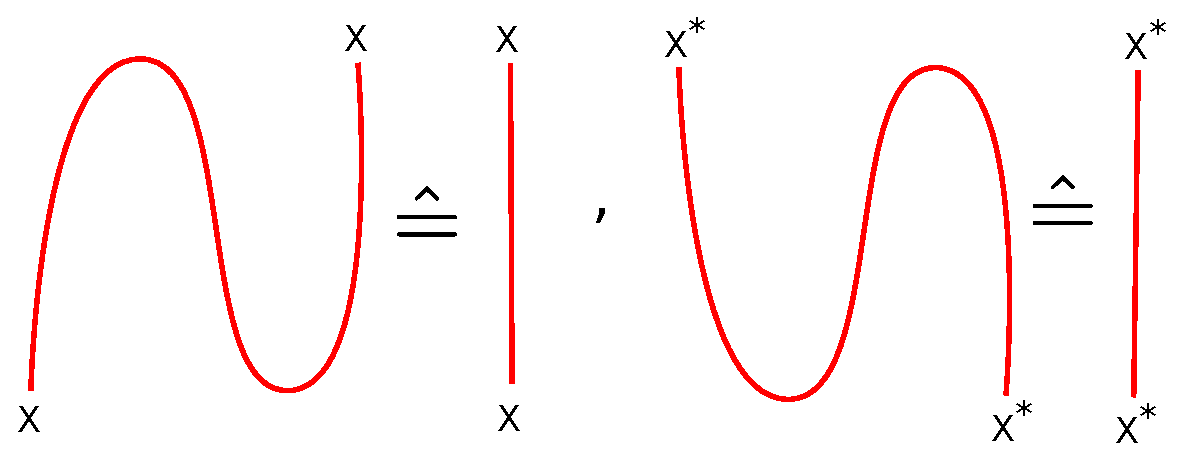
\includegraphics[width=0.6\textwidth]{snake.eps}
\end{center}
i.e., the following equations are satisfied, \begin{align}
	\label{rigid2}\id_X &= (\id_X \otimes \ev_X) \circ(\coev_{X} \otimes \id_X),\\ \label{rigid1}\id_{X^*} &= (\ev_X\otimes \id_{X^*})\circ(\id_{X^*}\otimes \coev_X).
\end{align}

\end{Def}

The object $X^*$ is called the \textit{left dual} of $X$. A \textit{right rigid} structure with a \textit{right dual} ${}^*X$ for each $X\in \C$ is defined similarly. The object $X$ is the right dual of $X^*$ and the left dual of ${}^*X$. Left (or right) duals are unique upto a unique isomorphism. Suppose an object $X$ has 2 left duals $X_1^*$ and $X_2^*$, then there is an isomorphism \begin{equation*}
	X_1^* \xrightarrow{\id \otimes \coev_2} X_1^* \otimes X\otimes X_2^*  \xrightarrow{\ev_1 \otimes \id} X_2^*.
\end{equation*}

\begin{Def}\label{fstar}
For a morphism $f:X\rightarrow Y$, its \textit{dual morphism} $f^*: Y^* \rightarrow X^*$ is defined as 
\begin{equation}
	f^*:Y^*\xrightarrow{\id\otimes \coev_X} Y^* \otimes X\otimes X^* \nonumber  \xrightarrow {\id \otimes f \otimes \id} Y^* \otimes Y \otimes X^* \xrightarrow{\ev_Y \otimes \id_{X^*}} X^*.
\end{equation}
\end{Def}
Graphically, $f^*$ is represented in terms of $f$ as the following diagram.
\begin{center}
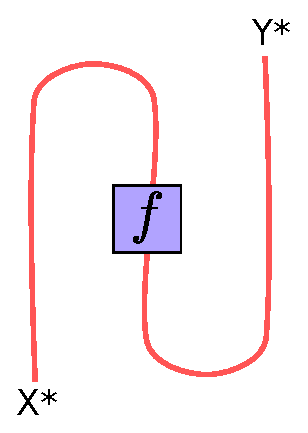
\includegraphics[width=0.15\textwidth]{fdual.eps}
\end{center}
Knowing that tensoring is graphically represented by juxtaposition, it is also easy to see from this diagram that there is an isomorphism $J_{X,Y}: (X\ot Y)^* \cong Y^* \ot X^*$. The object $\one$ is self dual and it is easily checked that the data $(*, J, J_1)$ verifies the coherence conditions for a monoidal functor.
\begin{Prop}
Given a strict tensor functor $F:\C \rightarrow \D$, with structure morphisms in $\D$, \begin{align}
	&J_{X,Y} : F(X) \otimes F(Y) \rightarrow F(X\otimes Y)\\
	&J_1 : \one \rightarrow F(\one),
\end{align}
and an object X with a left dual $X^*$, the object $F(X^*)$ is a left dual of $F(X)$ with evaluation and coevaluation maps given by
\begin{align}
	\ev_{F(X)}: F(X^*)\otimes F(X) \xrightarrow{J_{X^*, X}} F(X^*\otimes X) \xrightarrow{F(\ev_X)}F(\one) \xrightarrow{J_1} \one\\
	\coev_{F(X)}: \one \xrightarrow{J_0} F(\one) \xrightarrow{F(\coev_X)} F(X\otimes X^*) \xrightarrow{J_{X, X^*}} F(X) \otimes F(X^*).
\end{align}
\end{Prop}
We skip the details of the proof as they are routine and not essential to what follows.
\begin{Prop}
Let $U, V, W$ be objects having duals in a strict tensor category $\C$, and let $g: U\rightarrow V$, $ f:V\rightarrow W$ be morphisms in $\C$. Then $(f \circ g)^* = g^*\circ f^*$.
\end{Prop}
\begin{proof}
We prove this by graphical calculus,
\begin{center}
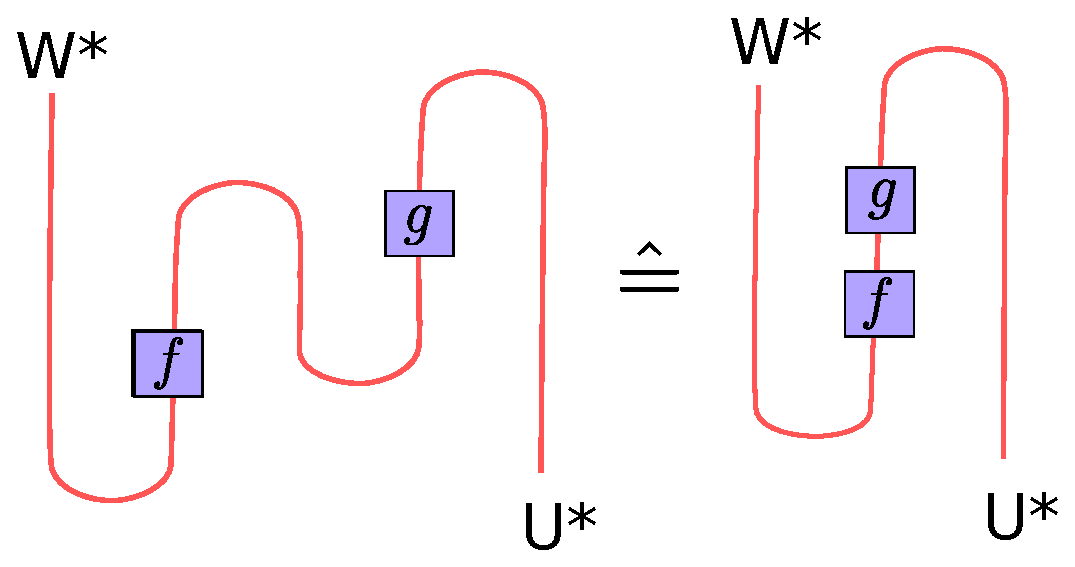
\includegraphics[width=0.5\textwidth]{dualcomposition.eps}
\end{center}
where we use equation (\ref{rigid2}) for the object $V^*$.
\iffalse
Consider the following map 
\begin{align}
\theta:  U \xrightarrow{g} V \xrightarrow{ \coev_V \ot \id_{V}}    (V \ot V^*) \ot V \nonumber\\\xrightarrow {\alpha_{V, V^*, V}} V\ot (V^*\ot V) \xrightarrow{\id_V \ot \ev_V} V \xrightarrow{f} W 
\end{align}
If $\Theta := \id_{W^*}\otimes \theta \otimes \id_{U^*}$, then the map \begin{align}
W^* \xrightarrow{\id_{W^*}\otimes \coev_U} W^* \otimes (U \otimes U^*)\xrightarrow{\alpha_{W^*, U, U^*}} (W^* \otimes U)\otimes U^* \nonumber\\\xrightarrow{\Theta } (W^*\otimes W) \otimes U^* \xrightarrow{\ev_W \otimes id_{U^*}} U^*\label{dualmor}
\end{align}
is by definition $g^*\circ f^*$. However, since $V^*$ is dual to $V$, the composition
\begin{equation*}
	V \xrightarrow{ \coev_V \ot \id_{V}}    (V \ot V^*) \ot V \nonumber\\\xrightarrow {\alpha_{V, V^*, V}} V\ot (V^*\ot V) \xrightarrow{\id_V \ot \ev_V} V
\end{equation*}
equals $\id_V$.
The map $\theta$ is then simply $f\circ g$ and the map \ref{dualmor} becomes $(f\circ g)^*$.
\fi
\end{proof}

\subsection{Fusion categories}
\begin{Def}
A locally finite semisimple rigid tensor category  $\C$ such that $\OO(\C)$ is finite and $\one$ is simple is called a \textit{fusion category}.
\end{Def}
The rigid structure on arbitrary tensor categories can be quite complicated to understand but in the setting of fusion categories it behaves rather nicely.
\begin{Prop}\label{doublestar}
In a fusion category, for every simple object $V$ there is an isomorphism $V\xra{\sim} V^{**}$.
\end{Prop}
\begin{proof}
There are maps $V\otimes {}^*V\rightarrow \one$ and $\one \rightarrow V\otimes V^* $. Since the category is semisimple, there is an injection  $ \one \rightarrow V\otimes {}^*V$, and a projection $V\otimes V^*\rightarrow \one$, and so the left dual is isomorphic to the right dual, $V^*\cong {}^*V$, and hence $V\cong V^{**}$.
\end{proof}
In fact, the isomorphism in the last proposition is functorial: for every $f:V\ra W$, we define $f^{**}$ to be the dual of the dual morphism of $f$ (see Definition \ref{fstar}).\\
Rigidity lets us define the notion of the trace of a morphism in a rigid monoidal category. For $V\in \C$, a rigid monoidal category,  $f\in \Hom(V, V^{**})$, the \textit{left trace}  is defined as \begin{align}
\tr_L(f): \one \overset{\coev_V}\longrightarrow V\otimes V^{*} \overset{f\otimes \id_V^*}\longrightarrow V^{**} \otimes V^* \overset{\ev_{V^*}}\longrightarrow \one \end{align} 
\begin{center}
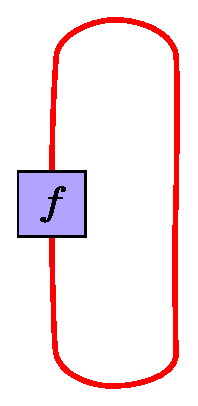
\includegraphics[width=0.08\textwidth]{lefttrace.eps}
\end{center}

Similarly, for $f: V^{**} \rightarrow V$, the \textit{right trace} is defined as
\begin{align}
\tr_R(f): \one \overset{\coev_{V^*}}\longrightarrow V^*\otimes V^{**} \overset{\id_{{}^*V}\otimes f}\longrightarrow V^* \otimes V \overset{\ev_{{}^{**}V}}\longrightarrow \one  
\end{align}
\begin{center}
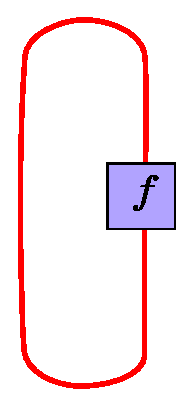
\includegraphics[width=0.08\textwidth]{righttrace.eps}
\end{center}

 
The left and right trace are related as $\tr_L(f) = \tr_R(f^*)$.
\subsubsection{Fusion rings}
Let $\C$ be a fusion category. The operations $\otimes$ and $\oplus$ along with the decomposition \eqref{fusionrule} equip the Grothendieck ring $K(\C)$ of $\C$ with the structure of a \textit{unital based ring} (see \cite[Section 3.1]{EGNO}) with basis $\OO(\C)$. We will refer to $K(\C)$ along with this unital based ring structure as the \textit{fusion ring} of $\C$.
\begin{Def}
A \textit{pointed} fusion ring is a fusion ring where every simple object is invertible, i.e., for every object $X\in \OO(\C)$, there is a $Y\in \OO(\C)$ isomorphic to $X^*\in \C$ (and by the proof of \ref{doublestar} also to ${}^*X\in \C$) such that \begin{equation*}
	X\ot Y = \one, Y\ot X = \one.
\end{equation*} 
\end{Def}

\begin{Def}
A \textit{hyperring} is a fusion ring with all multiplicities either 0 or 1.
\end{Def}
A pointed fusion ring is an example of a hyperring.

\begin{Def}
A fusion ring is \textit{singly generated} by an object $X\in \OO(\C)$ if every other element of $\OO(\C)$ has positive multiplicity in $X^{\otimes n}$ for some $n>0$.
\end{Def}
We give several examples of singly generated hyperrings in Section \ref{results}.

\begin{Def}
 A \textit{near-group} fusion ring is a fusion ring with all simple objects invertible except one which we call $X$, such that $N^X_{XX} = m$ for $m\geq	0$, and $N^{I}_{XX} =1$ for all invertible objects $I$. When $m=0$, the fusion ring is called a \textit{Tambara-Yamagami} fusion ring. 
 \end{Def} 
Tambara-Yamagami fusion rings and near-group fusion rings with $m=1$ are further examples of hyperrings. Both near-group and Tambara-Yamagami fusion rings are singly generated.\\
For a fusion ring $R$ let $g(R)$ denote its group of invertible objects.
\begin{Def}
For two fusion rings $R$ and $S$, their \textit{direct product} $R\times S$ is the fusion ring consisting of pairs $(r, s)$ for $r \in R$ and $s\in S$, with $(r, s)* (r', s') := (r* r', s* s')$, where $*$ is either $\oplus$ or $\ot$. The \textit{semidirect product} $R\semidir S$ is the fusion ring consisting of pairs $(r, s)$ with $(r, s)\oplus (r', s') := (r\oplus r', s\oplus s')$ and $(r, s)\ot (r', s') := (r\ot \varphi(s)r', s \ot s')$, where $\varphi:S\ra \Aut(R)$ is a map such that $\varphi|_{g(S)}$ is a group homomorphism and $\varphi(s) = \id_R$ if $s$ is not invertible. 
\end{Def}
\subsubsection{Pivotality}
\begin{Def}
	A \textit{pivotal structure} on a rigid monoidal category is a monoidal functorial isomorphism from the identity functor to the double dual functor \begin{equation*}
	j:  \id\rightarrow {}^{**} .
\end{equation*}

\end{Def}Our primordial example $\Vect$, is an example of a pivotal category, where the pivotality is a result from elementary linear algebra, with the isomorphism $V\rightarrow V^{**}$ explicity described by \begin{equation*}
	v\mapsto v' ,\quad  \text{such that} \quad v'(?) = ?(v)
\end{equation*}  for $v\in V$, where $?$ stands for any element in $V^*$. An example of a category without a pivotal structure is the category $\Rep H$, for the Hopf algerbra $H = \mathcal{B}(V_3) \# \kk S_3$, where $\mathcal{B}(V_3)$ is a Nichols algebra, for details see \cite[Remark 2.11]{MR3585364}.
The following is an important open question in the theory of fusion categories. \begin{Conj}[Etingof-Nikshych-Ostrik]
Every fusion category admits a pivotal structure.
\end{Conj}
%In a pivotal category, the pivotal structure on an object $X$, $j_X$ is related to the pivotal structure on its dual as \begin{equation*}	(j_X)^{*-1} = j_{X^*}.\end{equation*} 


\begin{Def}
A fusion category is \textit{spherical} with respect to a given pivotal structure $j$, if $\tr_L(f) = \tr_R(f)$ for $f \in \C(X, X)$.
\end{Def}
\begin{Def}
For an object $V$ in a spherical fusion category $\C$, we define its \textit{dimension} as $\dim (V) = \tr(\id_V)$.
\end{Def}

Let $\psi:\id\ra **$ be a functorial isomorphism in a fusion category $\C$ (note that $\psi$ is not tensor, and that such an isomorphism exists in any fusion category). Define \begin{align}
	\tr_+(f) = \tr_L(\psi_V\circ f)\\
	\tr_-(f) = \tr_R(f\circ \psi_V\inv)
\end{align}
for a morphism $f: V\rightarrow V$. We can define the M\"uger's squared norm for a $X\in \OO(\C)$ given by \begin{equation*}
	|X|^2 = \tr_+(\id_X)\tr_-(\id_X),
\end{equation*}
and since $X$ is simple, $\psi_X$ is unique upto a scalar, rendering the above definition of the squared norm invariant under the choice of $\psi$. \\ For an object $V$ in a spherical fusion category $|V|^2 = \dim (V)\dim (V^*) = \dim (V)\dim (V^*)$, and so $|V|^2 = (\dim V)^2$. 
\begin{Def}
The \textit{categorical} (or \textit{global}) \textit{dimension} of a fusion category is defined to be the sum of M\''uger's squared norms of its simple objects.
\end{Def}
\begin{Rem}\rm
Throughout this thesis, we will not distinguish between the quantities $\FPdim(X)$, $\dim(X)$ and $+\sqrt{|X|^2}$, since they are equal for any object in the categories we will consider.
\end{Rem}
\begin{Expl}\rm
Consider the category of finite dimensional representations of a finite group $G$, $\Rep(G)$, whose pivotal structure is inherited from $\Vect$, so the squared norm of an irreducible representation is the square of its vector space dimension. The categorical dimension of $\Rep(G)$ is \begin{equation*}
	\sum_{V_i\in \OO(\Rep(G))} (\dim V_i)^2 = |G|.
\end{equation*}
\end{Expl}
\subsubsection{Fusion subcategories and grading}
\begin{Def}
A \textit{fusion subcategory}  of a fusion category $\C$ is a full tensor subcategory $\C'\subset \C$ such that if $X\in \C$ is isomorphic to a direct summand of an object in $\C'$ then $X\in \C'$.
\end{Def}
\begin{Prop}
Every fusion subcategory of a fusion category is rigid.
 \end{Prop} 
\begin{proof}
The proof makes use of the following lemma which is proved in \cite[Lemma F.6]{MR2609644}.
\begin{Lem}\label{N}
For an object $X\in \OO(\C)$, there exists a positive integer $N$ such that $\Hom(\one, X^{\ot N}) \neq 0$.
\end{Lem}
Let $\D$ be a fusion subcategory of $\C$. If $X\in \OO(\D)$ then $X^{\ot n}\in \D$ for $n>0$. Consequently $\Hom(\one, X^{\ot N}) = \Hom(X^*, X^{\ot N-1})\neq 0$ where $N$ is as in the Lemma \ref{N}. Hence $X^*\in \OO(\D)$.
\end{proof}
 \begin{Def}
 The \textit{adjoint subcategory} of a fusion category $\C$ is the fusion subcategory $\C_{ad} \subset \C$ generated by objects of the form $X\otimes X^*$, for $X\in \OO(\C)$.
 \end{Def}
\begin{Def}
A \textit{grading} on a fusion category $\C$ by a group $G$ is a map \begin{equation*}
	\text{deg}: \OO(\C) \rightarrow G \label{deg}
\end{equation*}
such that if $Z\subset X\otimes Y$ then $\text{deg } Z = \text{deg } X\cdot \text{deg } Y$. A grading is \textit{faithful} if deg is surjective. 
\end{Def}

The grading yields a decomposition $\C = \bigoplus_{g\in G}\C_g$, where $\C_g$ is generated as a semisimple category by simple objects of degree $g\in G$. The term grading is also used to refer to this decomposition. By the multiplicativity of the map deg, it is easy to see that $\C_{ad}\subset \C_1$ for any $G$. There exists a \textit{universal grading group} $U_\C$ for any fusion category $\C$ such that if $\C$ is  faithfully graded by any other group $G$ then there is an epimorphism $U_{\C}\ra G$.

\begin{Expl}\rm\label{VecOmegaG}
A class of fusion categories very relevant to this thesis is of the form $\Vect^\omega_G$, where $G$ is a finite group and $\omega$ is a 3-cocycle with values in $\CC^\times$. The simple objects of $\Vect^\omega_G$ upto isomorphism are of the form $\delta_g$ for $g\in G$. The tensor product is defined as \begin{equation*}
	\delta_g\ot \delta_h \subseteq \delta_{gh},
\end{equation*} with the associator $\omega$ given by \begin{equation*}
	\omega(g, h, k): (\delta_g \ot \delta_h)\ot \delta_k \ra \delta_g \ot (\delta_h\ot \delta_k).
\end{equation*}
The fusion matrix of each simple $\delta_g$ is a permutation matrix, whose largest non-negative eigenvalue is 1, so each simple has dimension 1 and the categorical dimension of $\Vect^\omega_G$ is consequently $|G|$. It has a canonical pivotal structure since all its objects are vector spaces, and this pivotal structure is spherical. Its universal grading group is $G$. 
\end{Expl}

\subsubsection{Frobenius-Schur indicators}
For an object $X$ in a pivotal fusion category $\C$, the $n$-th Frobenius-Schur indicator is defined as the \begin{equation*}
	\nu_n(X) := tr(E_X^n),
\end{equation*} where $E_X^n\in  \End(\C(\one, X^{\ot n}))$ is defined below, considering $X^{\ot n}$ with all parentheses to the right.
\begin{center}
\includegraphics[width=0.4\textwidth]{fsi.eps}
\end{center}
For $n>0$, the Frobenius-Schur indicator is periodic, $\nu_n(X) = \nu_{n+r}(X)$, where $r$ depends on $X$ and is called the \textit{Frobenius-Schur exponent} of $X$. The Frobenius-Schur exponent of $\C$ is the lcm of the Frobenius-Schur exponents of all the simple objects of $\C$. The Frobenius-Schur indicators of objects in the Deligne product $\C\boxtimes \D$ of fusion categories $\C$ and $\D$ have the following property,
\begin{equation}\label{fsideligne}
	\nu_n(X\boxtimes Y) = \nu_n(X)\nu_n(Y),
\end{equation} for $X\in \C$ and $Y\in \D$.


\subsection{Pointed fusion categories}\label{pfc}
Perhaps the simplest examples of fusion categories are the so-called \textit{pointed fusion categories}, which are fusion categories with pointed fusion rings. In other words, a pointed fusion category $\D$ is such that $\D_{ad}$ is generated by $\one$. Objects in  $\OO(\D)$ form a group $G$ under the $\ot$ operation. This induces a grading on $\D$ by $G$, with each homogeneous component generated by an element of $\OO(\D)$.  The fusion matrix for each simple object is a permutation matrix, whose largest non-negative eigenvalue is 1, so each simple object has dimension 1. 
Define the associator on a triple of simple objects\begin{equation*}
	\omega(g,h,k):(X_g \otimes X_h) \otimes X_k \rightarrow    X_g \otimes (X_h\otimes X_k)
\end{equation*} for $g, h, k \in G$. 
 Each $\omega(g,h,k)$ is an isomorphism between 1-dimensional vector spaces, and is given by an element of $\GL_1(\kk) = \kk^\times$.  The fact that $\omega$ must satisfy the pentagon axiom leads to the condition \begin{equation*}
	\omega(g,h, kl)\omega(gh, k, l) = \omega(h,k,l)\omega(g, hk, l)\omega(g,h,k).
\end{equation*} This is exactly the condition for a 3-cocycle in group cohomology, so $\omega \in Z^3(G, \CC^\times)$.  A similar argument for the unit axioms gives the condition that $\omega$ is a normalized 3-cocycle, which means $\omega(g, h, k)=1$ if either $g, h$ or $k$ is 1. One can establish a tensor equivalence \begin{equation*}
	(F, \eta, \eta_1): \D \rightarrow \Vect^\omega_G,
\end{equation*} where the functorial isomorphism $\eta_{X_g,X_h}: F(X_g)\otimes F(X_h) \rightarrow F(X_g\otimes X_h)$ is the identity for any $g, h\in G$.  We have thus shown that any pointed fusion category is equivalent to $\Vect^\omega_G$ where $\omega$ is a 3-cocycle and $G$ is a finite group. 
\begin{Rem}\rm
Given two pointed fusion categories $\Vect^\omega_G$ and $\Vect^{\omega'}_G$ such that $\omega $ and $\omega'$ are cohomologous, we may establish a tensor equivalence \begin{equation}
	(F, \eta, \eta_1): \Vect^{\omega'}_G \rightarrow \Vect^\omega_G,
\end{equation} where $\eta(\delta_g, \delta_h) = \gamma(g, h)$, where $\gamma$ is a normalized 2-coboundary with values in $\kk^\times$.
\end{Rem}

\section{Module categories and categorical Morita equivalence}\label{section:module-categories}
\begin{Def}\rm\label{modulecategorydef}
A left module category $\M$ over a fusion category $\C$ is a semisimple locally finite category $\M$ with a finite number of simple objects,  together with a bilinear functor $\otimes^{\M}: \C\times \M\ra \M$ along with natural isomorphisms \begin{align}
	\beta_\M &: \otimes^{\M} \circ (\otimes ^{\C} \times \id_{\M})\cong  \otimes^{\M} \circ (\id_{\C} \times \otimes^{\M})\\
	l_\M &: (\one \otimes^{\M} - ) \cong \id_{-}
\end{align}
satisfying the pentagon and triangle identities for object $X, Y, Z \in \C$ and $M\in \M$.
\[
  \xymatrix{&  X\otimes^\M (Y\otimes^\M (Z \otimes^\M M)) & \\ 
  X\otimes^\M ((Y\otimes^\C Z) \otimes^\M M) \ar[ru]^{\id_X \otimes^\M (\beta_{Y, Z, M})} &  & (X\otimes^\C Y)\otimes^\M (Z \otimes^\M M))\ar[lu]^{\beta_{X, Y, Z\otimes^\M M}}\\ 
  (X\otimes^\C (Y\otimes^\C Z)) \otimes^\M M \ar[u]_{\beta_{X, Y\otimes Z, M}} &  &  \ar[ll]^{\alpha_{X, Y, Z}\otimes^\M M} ((X\otimes^\C Y)\otimes^\C Z) \otimes^\M M\ar[u]^{\beta_{X\otimes Y, Z, M}} }
\]
\[
\xymatrix{(X\otimes^\C \one) \otimes^\M M \ar[rr]^{\beta_{X, \one, M}}\ar[dr]^{r_X} && X\otimes^\M(\one \otimes^\M M)\ar[dl]^{l^\M_M}\\
& X\otimes M }
\]
\end{Def}

\begin{Rem}\label{modulecategorydefremark}\rm
Alternatively, it can also be defined as a semisimple locally finite category $\M$ with a finite number of simple objects, carrying the additional data of a $\kk$-linear monoidal functor $F:\C\rightarrow \End(\M)$, where $\End(\M)$ denotes the category of $\kk$-linear endofunctors of $\M$, where the tensor product structure is given by composition.
\end{Rem}
\begin{Prop}
The definitions of a $\C$-module category from \ref{modulecategorydef} and \ref{modulecategorydefremark} are equivalent.
\end{Prop}
\begin{proof}
Let $F:\C\rightarrow \End(\M)$ be the functor from Remark \ref{modulecategorydefremark}. One can define the module category structure $\otimes^{\M}$ as \begin{equation*}
	X\otimes^{\M} M := F(X)(M)
\end{equation*}
The isomorphism $(X\otimes^\C Y)\otimes^\M M\rightarrow X\otimes^\M (Y\otimes^\M M)$ for $X, Y \in \C$ is given by \begin{equation}\label{moddef2}
	(X\otimes^\C Y)\otimes^\M M := F(X\otimes Y)(M) \xrightarrow{J\inv_{X, Y}(M)} F(X)\circ F(Y)(M) =: X\otimes ^\M (Y\otimes^\M M )   
\end{equation}
In the other direction, If $\M$ is a $\C$-module category, then for $X\in \C$, \begin{equation*}
	M\rightarrow X\otimes^\M M
\end{equation*}
defines an endofunctor of $\M$, with the monoidal structure defined using the associativity constraint $m_{X, Y, M}$.
\begin{equation}\label{moddef1}
	F(X)\circ F(Y)(M):= X\otimes^\M (Y \otimes^\M M) \xrightarrow{m\inv_{X, Y, M}} (X\otimes^\C Y) \otimes^\M M=: F(X\otimes^\C Y) \otimes^\M M 
\end{equation} It is straighforward to verify the pentagon and triangle axioms for both the definitions.
\end{proof}
Similar definitions can be written down for a right $\C$-module category, and also for a $\C-\D$-bimodule category, where $\D$ is also a fusion category. From now on we will stop labeling the tensor product with the respective category, banking on the fact that this will be clear from context.
There is a notion of direct sum of module categories.
\begin{Prop}
For module categories $\M$ and $\NN$ over a fusion category $\C$, their \textit{direct sum} $\M\oplus\NN$ is a module category over $\C$ with the action and the associativity and unit constraints defined as sums of those of $\M$ and $\NN$ .
\end{Prop}
The proof of this statement is a routine verification of conditions and we skip it.
\begin{Def}
	A module category $\M$ over a fusion category $\C$ is \textit{indecomposable} if it cannot be decomposed as a direct sum of non-trivial module categories.
	\end{Def}	

\begin{Rem}\rm
Let $\M$ be a module category over a fusion category $\C$. Then we have the following isomorphisms \begin{equation*}
	\Hom(X\ot M, N)\cong \Hom(M, X^*\ot N), \quad \Hom(M, X\ot N)\cong \Hom(X^*\ot M, N).
\end{equation*}
This is easy to see graphically, where we may make the following identifications.

\begin{center}
\includegraphics[width=0.6\textwidth]{dualhom.eps}
\end{center}

\end{Rem}

\begin{Expl}\rm
Every semisimple category $\M$ is a $\Vect-\Vect$-bimodule category in a unique way. Let $X\in \C$ and $V \in \Vect$, then $V\cong \kk^n$ for some positive integer $n$, and so the left module structure is given as\begin{align}
	\Vect \times \M & 	\ra \M\\
	V\otimes X & 	\ra X^{\oplus n},
\end{align} and similarly for the right module structure.
\end{Expl}
\begin{Expl}\rm
Any fusion category $\C$ is itself naturally a $\C-\C$-bimodule category, or equivalently a left $\C \boxtimes \C^{op}$ module category, where $\boxtimes$ denotes the Deligne tensor product, and \textit{op} denotes the flipped monoidal product.
\end{Expl}
\begin{Expl}\rm
For $G$ a finite group, $\Vect$ is a left $\Rep(G)$-module category, where an object $V\in \Rep(G)$ acts by $F(V)\otimes -$, where $F:\Rep(G)\rightarrow \Vect$ denotes the forgetful functor. 
\end{Expl}
\begin{Expl}\rm
For any algebra object $A$ in a fusion category  $\C$, the category $\Mod_C-A$ of right $A$-modules in $\C$ is a left $\C$-module category, for details see Theorem \ref{Ostrik}.
\end{Expl}
\begin{Def}
A $\C$-module functor $F:\M\rightarrow \NN$ is a functor $F:\M\rightarrow \NN$ along with a functorial isomorphism \begin{equation*}
	s_{X, M}: F(X\otimes M) \rightarrow X\otimes F(M)  
\end{equation*} for $X\in \C$ and $M\in \M$, such that the following diagrams commute. 
\[
\xymatrix{
& F((X\ot Y) \ot M) \ar[rd]^{F(m_{X, Y, M})} \ar[ld]^{s_{X\ot Y, M}}& \\
(X\ot Y) \ot F(M) \ar[d]^{m'_{X, Y, F(M)}} & &  F(X \ot (Y\ot M))\ar[d]^{s_{X, Y\ot M}} & \\
X\ot (Y \ot F(M))& & X \ot F(Y\ot M)\ar[ll]^{s_{Y, M}} }
\]
\[
\xymatrix{F(\one\ot M) \ar[rr]^{s_{\one, M}} \ar[rd]^{F(l_M)}& &  \one \ot F(M)\ar[ld]^{l_{F(M)}}\\
& F(M) & }
\]
\end{Def}
\begin{Def}
A \textit{ $\C$-module functorial morphism} $\nu$ between functors $(F,m)$ and $(G, n)$ is a functorial morphism $\nu:F\rightarrow G$ that is natural with respect to the module functor structure, i.e., \[
	\xymatrix{
  	F(X\otimes M) \ar[d]_{\nu_{X\otimes M}}\ar[r]^{s_{X, M}} & X\otimes F(M)\ar[d]^{\nu_X \otimes \id_M}\\
   G(X\otimes M)	 \ar[r]^{s'_{X, M}} & X\otimes G(M).}			
\]

\end{Def}
$\C$-module functors between $\C$-module categories $\M$ and $\NN$ form a category, with morphisms being $\C$-module functorial morphisms.
\subsection{Module categories over $\Vect^\omega_G$}
We will now discuss the module categories over $\Vect^\omega_G$. A module category $\M$ over $\Vect^\omega_G$ comes equipped with auto-equivalences \begin{align}
F_g:\M &\ra \M\label{autoeq}\\F_g(M) &= \delta_g \otimes M\nonumber
\end{align} and functorial isomorphisms $\eta(g, h)$, for every $g,h \in G$. \begin{equation*}
	\xymatrix{F_g\circ F_h (M) \ar[rr]^{\eta(g, h)(M)}\ar[d]_{F_g\circ F_h(f)} && F_{gh}(M) \ar[d]^{F_{gh}(f)} \\
	F_g\circ F_h(N) \ar[rr]^{\eta(g,h)(N)} && F_{gh}(N)} 
\end{equation*}  for objects $M, N \in \M$ and $f\in \Hom(M, N)$. If we have the composition of auto-equivalences $F_g\circ F_h\circ F_k$ associated with elements $g,h, k \in G$, then by the pentagon axiom of a module category, the two ways of passing to the autoequivalence $F_{ghk}$ must be isomorphic. This imposes a  condition on $\eta$.

\begin{equation*}
	\eta(g, h)\eta(gh,k) = \omega(g, h, k)\eta(h,k)\eta(g, hk)
\end{equation*}

For a simple object $M$ in an indecomposable module category $\mathcal{M}$ over $\Vect^\omega_G$,  $\delta_g \otimes M$ is also a simple object for $\delta_g \in \Vect^\omega_G$. Suppose on the contrary that $\delta_g \otimes M$ decomposes as a direct sum, then by acting with $\delta_{g\inv}$ we get a decomposition for $M$. Since $\M$ is indecomposable this action of $G$ must be transitive, for if this were not the case, then each orbit of $G$ would be an indecomposable category and $\M$ would decompose as a non-trivial direct sum. The autoequivalences $F_g$ endow the set of simples $\OO(\M)$ with a transitive $G$-set structure. By the orbit-stabilizer theorem,  the stabilizers $L, L'$ of two distinct elements $x, x'=gx$ of a transitive $G$-set are conjugate in $G$, $L = g\hit L = gL'g\inv$. For the trivial $L$-module $\kk^\times$, consider
\begin{equation*}
	\Coind^G_L \kk^\times = \Hom_L(G,\kk^\times)\simeq \text{Fn}(G/L, \kk^\times),
\end{equation*}
i.e., functions from $G/L$ to $\kk^\times$. It has a left $G$-module structure,  $g\cdot f(x) = f(g\inv x)$ for an $L$-linear map $f:G\rightarrow \kk^\times$.
The associator for the module structure  $\beta_\M (\delta_g,\delta_h,M): (\delta_g\ot \delta_h)\ot M\rightarrow \delta_g\ot (\delta_h\ot M)$  is given by a function $m:G\times G \times G/L\rightarrow \kk^\times,$ where $M$ corresponds to the class $[b]\in G/L$, such that
\begin{equation}\label{pent}
	\omega(g,h,k)m(g, hk, b)m(h, k, b) = m(gh, k, b)m(g, h, kb)
\end{equation}

Associate with $\M$ a function $\Psi: G\times G \rightarrow \Coind^G_L \kk^\times$ defined as
\begin{align}
	\Psi_{(g, h)}(b) &= m(g, h, h\inv g\inv b) \\
	\Psi_{(g,h)}(ghb) &= (gh)\inv\cdot\Psi_{(g,h)}(b) = m(g, h, b)
\end{align}
Using equation \eqref{pent}, we get the condition
\begin{align}
	\Psi_{(gh, k)}\Psi_{(g, h)}&= \omega(g, h, k)\Psi_{(g, hk)} g\cdot \Psi_{(h, k)}  ,
\end{align}
where the multiplication is pointwise. \\Let $F:\M\ra\M'$ be an equivalence of $\Vect^\omega_G$-module categories with associated functions $\Psi: G\times G \rightarrow \Coind^G_L \kk^\times $ and $\Psi': G\times G \rightarrow \Coind^G_{L'} \kk^\times$ respectively. It has structure isomorphisms \begin{equation*}
	s_{\delta_g, M}: F(\delta_g \ot M)\ra \delta_g\ot F(M)
\end{equation*} given by a function $\xi: G\ra \text{Fn} (G/L, \kk^\times)$. In particular, $F$ is map of transitive $G$-sets from $\OO(\M)$ to $\OO(\M')$ and consequently, $L$ and $L'$ are conjugate and $F(\Psi_{(g, h)}) = \Psi_{(x\hit g, x\hit h)} =: \Psi^x_{(g, h)}$ where $x\in G$ is such that $L=x\hit L'$. The pentagon axiom from Definition \ref{modulecategorydef} gives the condition \begin{equation}
	\Psi_{(g, h)}^x  = \Psi'_{(g, h)} \xi(g)\xi(h)\xi(gh)\inv.\label{Fbigpsi}
\end{equation} As $\Psi$ and $\Psi'$ differ by a 2-coboundary, $F_x$ maps $\Psi$ to another element in its class in $H^2(G, \Coind^G_L k^\times)$.  Now, by Shapiro's lemma, we have the isomorphism
\begin{align*}
 	H^2(G, \Coind^G_L \kk^\times) &\overset{\sim}\longrightarrow H^2(L, \kk^\times)\\
 	[\Psi] &\mapsto [\Psi|_L].
 \end{align*} 
Denote $\Psi|_L$ by $\mu$. Similar to \eqref{Fbigpsi}, we have \begin{equation*}
	F_x(\mu(g, h)) = \mu(x\hit g, x\hit h) =: \mu^x(g, h) = \mu'(g, h) \xi(g)\xi(h)\xi(gh)\inv
\end{equation*} for $g, h\in L$ and $\xi:L\ra \kk^\times$, so $\mu$ and $\mu'$ are cohomologous. We thus have the following theorem.
\begin{theorem}\label{simpleparam}
A semisimple indecomposable $\Vect^\omega_G$-module category is determined by ($H,\mu$), where $H$ is a subgroup of $G$ and $\mu$ is a 2-cochain with values in $\kk^\times$ such that $\omega|_{H\times H\times H} = d\mu$. Two pairs $(H, \mu)$ and $(H', \mu')$ correspond to equivalent module categories if and only if $H' = g\hit H$ and $\mu^g$ is cohomologous to $\mu'$.
\end{theorem}

\subsection{Algebra objects in fusion categories and Ostrik's theorem}
Let $\C$ be a fusion category.
\begin{Def}\label{algdef}
 An algebra object $(A, \nabla, u)$ is an object $A\in \C$ together with morphisms $\nabla:A\otimes A \rightarrow A$  and $u: \one\rightarrow A$ such that the following diagrams commute.
\[
\xymatrix{(A \otimes A) \otimes A \ar[d]_{\nabla \otimes \id_A} \ar[rr]^{\alpha_{A, A, A}}& & A\ot (A\ot A)\ar[d]^{\id_A\otimes \nabla}\\
A\otimes A \ar[rd]_{\nabla} & & A\otimes A\ar[ld]^{\nabla}\\
& A & }
\]
\[
\xymatrix{ \one \ot A\ar[d]^{u\ot \id_A} \ar[r]^{l_A} & A\ar[d]^{\id_A} \\
A\ot A \ar[r]^{\nabla} & A
}
\xymatrix{  A\ot \one \ar[d]^{ \id_A\ot u} \ar[r]^{r_A} & A\ar[d]^{\id_A} \\
A\ot A \ar[r]^{\nabla} & A
}
\]
\end{Def}

\begin{Expl}\rm
In any fusion category, the unit object $\one$ is naturally an algebra object.
\end{Expl}

\begin{Expl}\rm
In a pointed fusion category $\Vect^\omega_G$, consider the the semisimple object $\CC_\mu H$, the twisted group algebra on $H$, a subgroup of $G$, by $\mu \in C^2(H, \CC^\times)$, with the product map given by \begin{align*}
	\nabla:\CC_\mu H \ot \CC_\mu H \ra \CC_\mu H\\
	\nabla(\delta_{h_1}, \delta_{h_2}) = \mu(\delta_{h_1}, \delta_{h_2})\delta_{h_1}\delta_{h_2}.
\end{align*} The axioms of an algebra object impose the condition that $\mu$ be normalized and $d\mu=\omega|_{H^3}.$
\end{Expl}
\begin{Expl}\rm\label{canonicalalg}
Objects of the form $X\otimes X^*$ for $X\in \C$, a fusion category, are algebra objects, with multiplication $\nabla = \id_X \otimes \ev_X \otimes \id_{X^*}$, and $u = \coev_X$. Recall that these are the objects that generate the adjoint subcategory $\C_{ad}$ as a tensor category.
\end{Expl}

\begin{Def}
A right $(A, \nabla, u)$-module  $(M, p) \in \C$ is an object $M\in \C$ with the structure map $p: M \ot A\rightarrow M$ which is associative in the category, i.e., the following diagram commutes. \[
\xymatrix{
	(M \ot A)\ot A \ar[rr]^{\alpha_{M,A,A} } \ar[d]^{\nabla \ot \id_M} & &  M\ot (A \ot A)  \ar[d]^{\id_A \ot p}\\
	 M\ot A \ar[r]^p& M &  M\ot A\ar[l]_p
}
\]
\end{Def}
From now on we will drop the structure maps while denoting algebras or modules and invoke them wherever necessary. 
\begin{Rem}\label{leftmod}\rm
For a right $A$-module $M\in \C$, the object $M^*$ has the structure of a left $A$-module, given by the image of $p$ under the isomorphisms \begin{equation}
	\Hom(M\ot A, M) \cong \Hom(M^*, A^* \ot M^*) \cong \Hom(A\ot M^*, M^*).
\end{equation}
\end{Rem}
Given $A$-modules $M_1,M_2\in \C$, the space of $A$-module morphisms $\Hom_A(M_1, M_2)$ is a subspace of $\C(M_1, M_2)$, and thus we may talk about the $\kk$-linear category $\Mod_\C(A)$. 
\begin{Prop}\label{modcasemisimple}
 For a semisimple algebra object $A$ in a fusion category $\C$, $\Mod_\C(A)$ is a semisimple category.
 \end{Prop}
 \begin{proof}
 We will show that every object $M \in \Mod_\C(A)$ is projective. We use the fact that if $A$ is a semisimple algebra, then the product map $\nabla: A\otimes A \rightarrow A$ splits as a map of $A$-bimodules. Then $M = M\otimes_A A$ is a direct summand of $M\otimes_A A\otimes A= M\otimes A$. Now, the functor \begin{equation}
 	\Hom_A(M \otimes A, -) \cong \C(M, -)
 \end{equation}
 is exact because $M$ is a projective object in $\C$. Hence $M\otimes A$ is projective, and consequently so is $M\in \Mod_\C(A)$.
 \end{proof}
 
\begin{Prop}
There is a left $\C$-module structure on $\Mod_\C(A)$, \begin{align}
	\C \times \Mod_\C(A) &\ra \Mod_\C(A)\\
     (X, M) &\mapsto X\ot M,
\end{align}
\end{Prop}
\begin{proof}
The object $X\otimes M$ has a canonical structure of a right $A$-module, given by the following composition \begin{equation}
	p_{X\otimes M}: (X\otimes M) \otimes A  \xrightarrow{a_{X, M, A}} X\otimes (M \otimes A) \xrightarrow{\id_X \otimes p} X\otimes M.
\end{equation}
We need to finally check that \begin{equation}
	(X\otimes Y) \otimes M \cong X\ot (Y\otimes M) 
\end{equation} is an $A$-module morphism.

\[
\xymatrix{((X\otimes Y ) \ot M)\ot A \ar[rr]^{a_{X, Y, M} \ot A} \ar[d]^{a_{X\ot Y, M , A}} & & (X\otimes(Y\ot M)) \ot A \ar[d]^{a_{X, Y\ot M, A}}\\
(X\ot Y) \ot (M\ot A)\ar[dd]_{(X\ot Y)\ot m} \ar[rrd]^{a_{X, Y, M\ot A}}&  & X\ot ((Y \ot M) \ot A) \ar[d]^{X\ot a_{Y, M, A}}\\
& & X\ot(Y\ot(M\ot A)) \ar[d]^{X\ot(Y\ot m)}\\
X\ot (Y\ot M) \ar[rr]^{a_{X, Y, M}} & & (X\ot Y)\ot M
}
\]
The top pentagon commutes because $a$ is an associator, and the bottom square commutes because switching parentheses is functorial.
\end{proof}

\begin{Lem}\label{tensoralgebra}
For the algebra object $A=X\ot X^*$, $X^*\ot_A X\cong \one$.
\end{Lem}
The following proof is due to E. Meir.
\begin{proof}
We want to show that \begin{equation}
	X^*\ot X \ot X^* \ot X  \mathrel{\mathop{\rightrightarrows}^{\alpha}_{\beta}} X^*\ot X \ra \one
\end{equation} is a coequalizer for appropriate morphisms $\alpha$ and $\beta$. Consider a map \begin{equation}
	f: X^* \ot_A X \ra V
\end{equation} for some object $V$. This means there's a morphism $g:X^*\ot X\ra V$ such that \begin{equation}
X^*\ot X \ot X^* \ot X 	 \mathrel{\mathop{\rightrightarrows}^{\ev\ot g}_{g\ot \ev}}  V\ra 0.
\end{equation} 
Let $K=\ker (\ev)$, then $K\ot X^*\ot X + X^*\ot X \ot K$ lies in the kernel of $\ev_X\ot g = g\ot \ev_X$. Now consider the exact sequences \begin{align*}
	0\ra K \ra X^*\ot X \ra \one \ra 0\\
	0\ra K \ra X^*\ot X \ra \one \ra 0.
\end{align*} The maps $X^*\ot X \ot X^*\ot X \ra \one$ and $\ev$ both have kernel $K\ot X^*\ot X + X^*\ot X \ot K$, so the map $f$ factors through $\one$, and thus we have the claimed isomorphism.
\end{proof}
\begin{Prop}\label{Cmoduleeqv}\rm
For an object $X\in\C$ and $A=X\ot X^*$ we may establish an equivalence of $\C$-module categories \begin{align}
\C&\ra \Mod_\C(A) \\
Y&\mapsto Y\ot X^*\\
M\ot_A X& \mapsfrom M.
\end{align}
\end{Prop}
\begin{proof}
It is easy to see with the help of Lemma \ref{tensoralgebra} that the assignments above do indeed give an equivalence. 
\end{proof}
\begin{Def}
An algebra $A\in \C$ is \textit{indecomposable} if $\Mod_\C(A)$ cannot be written as a non-trivial direct sum of module categories. 
\end{Def}
\begin{theorem}[Ostrik]\label{Ostrik}
Let $\C$ be a fusion category. Every indecomposable left $\C$-module category $\M$ is equivalent to a category $\Mod_\C(A)$ for a semisimple algebra object $A\in\C$.
\end{theorem}
Before we prove this theorem, we need to define the internal Hom. 
For a module category $\M$, consider the functor \begin{equation}
	\M(-\otimes M, N): \C\rightarrow \Vect, X\mapsto \M(X\otimes M, N) 
\end{equation} for a fixed $M, N\in \M$. The representing object for this functor $\underline{\Hom}(M, N)$ is called the \textit{internal Hom} between $M$ and $N$. There is a natural isomorphism \begin{equation}
	\M(X\otimes M, N) \cong \C(X, \underline{\Hom}(M, N)).\label{internalhomiso}
\end{equation}
We state the following lemma without a proof. 
\begin{Lem}\label{internalhomexact}
 For an object $M\in \M$, the functor \begin{align}
 \underline{\Hom} (M, -) :  \M &\rightarrow \C\\
	 N &\mapsto \underline{\Hom}(M, N)
\end{align} is exact.
 \end{Lem} 
\iffalse \begin{proof}
 Consider an exact sequence \begin{equation}\label{internalhomseq}
	0\ra X\ra Y \ra Z \ra 0,
\end{equation}and let us apply the functor  $\C(B\ot M, -)$ for $B\in \C$ and $M\in \M$,
\begin{equation}
	0 \ra \C(B\ot M, X)\ra \C(B\ot M, Y) \ra \C(B\ot M, Z)\ra 0.
\end{equation}
This functor is exact because $\M$ is semisimple. Using the definition of the internal Hom, we now have, \begin{equation}
	0 \ra  \C(B,\underline{\Hom} (M, X))\ra \C(B,\underline{\Hom} (M, Y)) \ra \C(B,\underline{\Hom}(M, Z))\ra 0.
\end{equation}
Since $B\in \C$ is a projective object, the functor $\C(B, -)$ preserves exact sequences. Hence \begin{equation}
	0 \ra \underline{\Hom} (M, X) \ra \underline{\Hom} (M, Y) \ra \underline{\Hom}(M, Z)\ra 0,
\end{equation}
which proves the lemma.
 \end{proof}\fi
The object $\underline{\Hom} (M, M)\in \C$ for some $M\in\M$, has the structure of an algebra object in $\C$. Consider the map \begin{equation}
	\ac: \underline{\Hom} (M, M) \otimes M \rightarrow M
\end{equation} where the action of $\underline{\Hom} (M, M)$ is given by the $\C$-module structure. Hence, we get the multiplication on $\underline{\Hom} (M, M)$,   \begin{equation}
\nabla_M:	\underline{\Hom} (M, M)\otimes \underline{\Hom} (M, M) \rightarrow \underline{\Hom} (M, M).
\end{equation} which is a morphism such that \begin{equation}
	\ac\circ (\nabla_M\ot \id_M) \cong \ac\circ (\id_{\underline{\Hom} (M, M)}\ot \ac)
\end{equation}  We also have the canonical unit morphism \begin{equation}
	\one\rightarrow \underline{\Hom}(M,M),                                                  
\end{equation}which is the image of $\id_M\in \Hom_\M(M, M)$ under equation \ref{internalhomiso}, with $X=\one$. 
\\
The internal Hom has the following property.
\begin{Lem}\label{internalhomlemma}
For objects $X\in \C$, and $ M, N\in \M$ where $\M$ is a $\C$-module category,
\begin{equation}
\underline{\Hom}(M, X\otimes N) \cong X \otimes \underline{\Hom}(M, N).
\end{equation}
\end{Lem}
\begin{proof}
Let $Y$ be an object in $\C$, then using the definition of the internal Hom and the Hom-tensor adjunction, \begin{align}
	\C(Y, \underline{\Hom}(M, X\ot N)) \cong \M(Y\ot M,  X\ot N) \cong \M(X^* \ot (Y\ot M),  N) \\
	\cong \M((X^* \ot Y)\ot M,  N) \cong \C(X^* \ot Y, \underline{\Hom}( M,  N)) \cong \C(Y, X\ot \underline{\Hom}(M,  N)).
\end{align} 
\end{proof}

\begin{proof} [Proof of Theorem \ref{Ostrik}]
Let $A=\underline{\Hom} (M,M)$ for an object $M\in \M$. We need to show that the following adjunction \begin{equation}
	- \otimes_A M : \Mod_\C(A) \leftrightarrows  \M : \underline{\Hom}( M, -) 
\end{equation}is an equivalence. First, for any object $X\in \Mod_\C(A)$, we need to show that \begin{equation}
	\underline{\Hom}(M, X\otimes_A M) \cong X
\end{equation}
Using the property from Lemma \ref{internalhomlemma} and the fact that the internal Hom is exact in the second variable, we can construct the following commutative diagram, \begin{equation}\label{coequalizercommute}
	\xymatrix{\underline{\Hom}(M, X\otimes A \otimes M) \ar@<-.5ex>[r]_{(2)} \ar@<.5ex>[r]^{(1)}\ar[d]^{\sim} & \underline{\Hom}(M, X\otimes M) \ar[r]\ar[d]^{\sim} & \underline{\Hom}(M, X\otimes_A M)\ar@{-->}[d] \\
	X\otimes A \otimes \underline{\Hom}(M, M) \ar@<-.5ex>[r]_{(4)} \ar@<.5ex>[r]^{(3)} & X\otimes \underline{\Hom}(M,  M) \ar[r] & X\otimes_A \underline{\Hom}(M,  M)\cong X}
\end{equation} where $(1)$ is the morphism $\underline{\Hom}(M, r \otimes M)$, $(2)$ is the morphism $ \underline{\Hom}(M, X\otimes l)$, $(3)$ is the morphism $r\ot \underline{\Hom}(M,M)$ and $(4)$ is the morphism $\id_X \ot \nabla_A$, where $r$ is the right $A$-module structure on $X$, $l$ is the left $A$-module structure on $M$, and $\nabla_A$ is the multiplication in $A$.	

In the other direction, for every $Y \in \M$, we must show\begin{equation}
	 \underline{\Hom} (M,Y) \otimes_A M \cong Y.
\end{equation}
We have the following series of isomorphisms \begin{equation}
	\underline{\Hom}(M, \underline{\Hom} (M,Y) \otimes_A M) \cong \underline{\Hom} (M,Y)  \otimes_A \underline{\Hom}(M, M) \cong  \underline{\Hom} (M,Y)  \otimes_A A \cong \underline{\Hom} (M,Y)
\end{equation}
and since $\underline{\Hom}(M, -)$ is exact by Lemma \ref{internalhomexact}, we have the desired isomorphism.
\end{proof}

Two algebras $A, B \in \C$ are said to be \textit{Morita equivalent} if $\Mod_\C(A)$ is equivalent to $\Mod_\C(B)$. This gives the classical notion of Morita equivalence for $\C = \Vect$. 


We have an analog of the Eilenberg-Watts theorem for module categories.
\begin{theorem}\label{eilenberg-watts}
Let $\M$ and $\NN$ be $\C$-module categories, such that $\M=\Mod_\C(A)$ and $\NN=\Mod_\C(B)$ for $A, B\in \C$. Then there is an equivalence \begin{align}
	\Bimod_\C(A, B) &\rightarrow \Fun_\C(\M, \NN)\\
	M &\mapsto -\otimes_A M \\
	F(A) &\mapsfrom F
\end{align}
\end{theorem}
\begin{proof}
We only need to check that the compositions of the above functors in both ways are functorially isomorphic to the identity. In the one direction \begin{equation}
	M\mapsto -\otimes_A M \mapsto A\otimes_A M \cong  M.
\end{equation} In the other direction, \begin{equation}
	F\mapsto F(A) \mapsto -\otimes_A F(A).
\end{equation} Now we may replace the functor $\Hom(M, -)$ in the diagram (\ref{coequalizercommute}) by $F(-)$, 
\begin{equation}
	\xymatrix{F(X\otimes A \otimes M) \ar@<-.5ex>[r] \ar@<.5ex>[r]\ar[d]^{\sim} & F(X\otimes M) \ar[r]\ar[d]^{\sim} & F(X\otimes_A M)\ar@{-->}[d] \\
	X\otimes A \otimes F(M) \ar@<-.5ex>[r] \ar@<.5ex>[r] & X\otimes F(M) \ar[r] & X\otimes_A F(M)\cong X.}
\end{equation} and analogously claim that $F$ commutes with the $\ot_A$ operation, and so\begin{equation}
	-\otimes_A F(A) \overset{\sim}\longmapsto F(-\otimes_A A) \cong F.
\end{equation}
\end{proof}


\subsection{Dual categories and categorical Morita equivalence}
For a $\C$-module functor $F:\M\rightarrow \NN$, the right adjoint $G$ has a $\C$-module functor structure, defined in the following manner. \begin{align}
	\M(M, G(X\otimes N))\cong {\NN}(F(M), X\otimes N) \cong {\NN}({}^*X \otimes F(M), N) \\ \xrightarrow{~} \NN(F({}^*X\otimes M), N) \cong \M({}^*X\ot M, 	 G(N))\cong \M( M, X\ot	 G(N)),
\end{align}
where we have used (in order) the adjunction $F\dashv G$, the $\C$-module functor structure and the adjunction again. 
\begin{Prop}\label{dualfusion}
The category $\Fun_\C(\M, \M)$ is a fusion category.
\end{Prop}
\begin{proof}
A proof of this fact can be found in \cite[Theorem 2.15]{EtiNikOst:FC}.
\iffalse The monoidal product in this category is given by composition. Let $G$ denote the left adjoint of an endofunctor $F$, then $G$ is the left dual of $F$. The adjunction furnishes maps \begin{equation}
	\ev:G\circ F \ra \id, \quad \coev:\id\ra F\circ G,
\end{equation} which serve as the evaluation and coevaluation map respectively, and the compositions \begin{equation}
	F\xra{\ev F} FGF \xra{F\coev} F\quad \text{and}\quad  G\xra{G\coev}GFG\xra{\ev G}G
\end{equation}verify the snake identities. Similarly, the right dual is the right adjoint of $F$. The additive structure on this category is given by point-wise addition, i.e., \begin{equation}
	(F\oplus F') X = F(X) \oplus F'(X).	
\end{equation} The simple objects are the functors which map every simple object $X_i$ to another simple object $X_j$, by Theorem \ref{eilenberg-watts}. For example if some object $X= X_i \oplus X_j$ and $F(X_i) = X$ then $F(X_i) = X  = X_{i'} \oplus X_{j'} = F_1(X_i) \oplus F_2(X_i)$gives the decomposition of the functor $F$ into simples, where $F_1$ is the functor that maps $X_i$ to $X_{i'}$ and $F-2$ is the functor that Since the number of simples upto isomorphism is finite, so is the number of the functors $F_i$. Further the identity functor is clearly a simple object. Every space of morphisms in $\Fun_\C(\M, \M)$ is a subspace of morphisms in $\M$, and the morphism spaces are hence finite-dimensional.\fi
\end{proof}

\begin{Rem}\rm
Let $A\in \C$ be an algebra such that $\M = \Mod_\C(A)$, then by Proposition (\ref{eilenberg-watts}),  $\Fun_\C(\M, \M)$ is equivalent to $\Bimod_\C(A)\op$. We could also use this equivalence to prove Proposition \ref{dualfusion}, which for $\M=\Mod_\C(A)$ establishes an equivalence between $A$-bimodules and endofunctors of $\M$.
\end{Rem}
The category $\Fun_\C(\M, \M)$ is called the \textit{dual category of $\C$ with respect to $\M$} and we will often denote it by $\C^*_\M$. 
\iffalse
Consider $\M = \Mod_\C(A)$ as a right module category over $\D =\Bimod_\C(A)$, then \begin{equation}
	\M(M\ot X, N) \cong \D(X, \underline{\Hom}(M, N)) \cong \D(X, {}^*M\ot N),
\end{equation} for $X\in C, M, N \in\M$, where the internal Hom  object $\underline{\Hom}(M, N) \cong {}^*M \ot N\in\Bimod_\C(A)$. The object $B:=\underline{\Hom}(A, A)\cong {}^*A\ot A$ is an algebra object in $\D$, where ${}^*A$ has a left module structure as described in Remark \ref{leftmod}. 
\fi
For the regular $\C$-module category $\C$, we may establish the following equivalence, 
\begin{align}
	\C^*_\C\cong \C\op\\
	- \ot X \mapsfrom X\\
	F \mapsto F(\one)
\end{align} 
\begin{Prop}
The functor \begin{equation}\label{can}
	\mathrm{can} : \C \ra (C^*_\M)^*_\M
\end{equation} is a tensor equivalence.
\end{Prop}
\begin{proof}
By Theorem \ref{Ostrik}, there is an object $A\in \C$ such that $\M =\Mod_\C(A)$, and by Theorem \ref{eilenberg-watts}, $\C^*_\M \cong \Bimod_\C(A)\op$, and $(\C^*_\M)^*_\M$ is equivalent to the category of $B$-bimodules in $\Bimod_\C(A)$, where $B={}^*A \ot A$.
We have the composition \begin{equation}
	A\cong \one \ot A \xra{\coev_{{}^*A}\ot \id_A} {}^*A \ot A \ot A \xra{\id_{{}^* A}\ot \nabla} {}^*A \ot A = B,
\end{equation} that allows any $A$-module to be given a $B$-module structure, and so $(\C^*_\M)^*_\M \cong \Bimod_\C(B)$, and by an equivalence similar to Remark \ref{Cmoduleeqv}, we have \begin{align}
	C&\ra \Bimod_\C(B)\\
	X &\mapsto {}^*A \ot X \ot A.
\end{align}
Hence the functor can is an equivalence of categories.
\end{proof}
Two fusion categories $\C$ and $\D$ are Morita equivalent if $\C^*_\M \cong \D\op$ for some $\D$. 

\begin{theorem}[M\"uger]
Categorical Morita equivalence is an equivalence relation.
\end{theorem}
Categorical Morita equivalence is reflexive because a fusion category $\C$ is Morita equivalent to itself, via the equivalence \begin{align*}
	\C\op &\ra \C^*_\C,\\
	X&\mapsto -\ot X\\
	F(\one)&\mapsfrom F.
\end{align*}  It is symmetric by equation (\ref{can}). For a proof of transitivity (in a more general context than ours), we refer to \cite[Proposition 7.12.18]{EGNO}.

Starting from a fusion category $\C$, categories of the form $\C^*_\M$ yield new examples of fusion categories.

\begin{Expl}\rm
Let us consider the example of a pointed fusion category $\Vect_G$ for a finite group $G$, defined in \ref{pfc}. $\Vect$ is a left module category over $\Vect_G$, the action given by \begin{equation}
	X\ot V = \Forg(X)\ot V,
\end{equation} where objects $X\in \Vect_G, V\in \Vect$ and $\Forg$ is the forgetful tensor functor $\Vect_G \ra \Vect$. Every $\Vect_G$-linear endofunctor $F$ of $\Vect$ is completely determined by $F(\one)$, and isomorphisms \begin{equation}
	s_g: F(\delta_g\ot V) \xra{\sim}\delta_g\ot F(V),
\end{equation} for $V\in \Vect$ which obey the appropriate pentagon and triangle axioms (see Definition \ref{modulecategorydef}). Concretely, these can be described by a homomorphism $G\ra GL(V), g\mapsto s_g$, or in other words, by a representation of $G$ on the vector space $V$. Conversely, any such representation would automatically yield a $\Vect_G$-module endofunctor. Thus, the category $(\Vect_G)^*_{\Vect}\cong \Rep(G)$ as fusion categories and so $\Rep(G)$ and $\Vect_G$ are categorically Morita equivalent.
\end{Expl} 
\begin{Def}

A fusion category $\mathcal{C}$ is called \textit{group theoretical} if it is Morita equivalent to a pointed fusion category with respect to some indecomposable module category.
\end{Def}
 The above criterion for a fusion category to be group theoretical may be expressed more concretely: any group theoretical category (GTC) $\C$ is tensor equivalent to $(\Vect^\omega_G)^*_{\M(H, \mu)}$ where $\M(H, \mu)$ denotes the category of modules over the twisted group algebra $\kk_\mu H\in \Vect_G^\omega$, where $(H, \mu)$ are as in Theorem \ref{simpleparam}.  Evidently, such a category is described by the data $(G, H, \omega, \mu)$, and we will denote by $\C(G, H, \omega, \mu)$ the GTC associated with this data. Note that the two distinct group theoretical data may yield equivalent GTCs.
By the equivalence in Theorem \ref{eilenberg-watts} to \begin{equation}\label{gtbimod}
	(\Vect^\omega_G)^*_{\M(H, \mu)} = \Fun_{\Vect^\omega_G}(\M(H, \mu), \M(H, \mu)) \cong {}_{\CC_\mu H}(\Vect^\omega_G)_{\CC_\mu H}
\end{equation} 
Thus, the category $\C(G, H, \omega, \mu)$ is tensor equivalent to the category ${}_{\CC_\mu H}(\Vect^\omega_G)_{\CC_\mu H}$ consisting of objects in $\Vect^\omega_G$ that are bimodules over the twisted group algebra $\mathbb{C}_\mu H$ and morphisms between these objects that are $\CC_\mu H$-bimodule maps. 
\begin{Rem}\rm
For all our GTCs, we choose the canonical pivotal structure.
\end{Rem}
\begin{theorem}[Etingof-Nikshych-Ostrik]\label{adapted}
Two categories $\C(G, H, \omega, \mu)$ and  $\C(G, H, \tilde{\omega}, \tilde{\mu})$  such that $\tilde{\omega} = \omega d\eta$ and and $\tilde{\mu} =\mu (\eta|_{H^2}) d\chi$, where $\eta:G^2\rightarrow \CC^\times$ and $\chi:H\rightarrow \CC^\times$ are normalized cochains, are monoidally equivalent.\end{theorem}
\begin{proof}
We have seen that $\Vect^\omega_G\cong \Vect^{\tilde{\omega}}_G$ if $\tilde{\omega} = \omega d\eta$ for $\eta: G^2\rightarrow \CC^\times$, a normalized 2-cochain. Now, if $\mu(\eta|_{H^2})$ and $\tilde{\mu}$ differ by a 2-coboundary, then the algebra objects $\CC_{\mu\eta|_{H^2}}H$ and $\CC_{\tilde{\mu}}H$ are isomorphic, and so have equivalent module categories, and hence the corresponding GTCs are also equivalent.
\end{proof}
\begin{Cor}\label{natale}
Two categories $\C(G, H, \omega, \mu)$ and $\C(G, H, \omega d\eta, 1)$ are tensor equivalent, for a suitable choice of normalized cochain $\eta:G^2\rightarrow \CC^\times$.\end{Cor}
\begin{proof}

Let  $\tilde{\mu}:H^2\rightarrow \CC^\times$ be such that \begin{equation} 
	 \tilde{\mu} = \mu\eta|_{H^2},
\end{equation} then we can define \begin{equation}
	\eta(p,q) := \begin{cases} 1 & p,q \not\in H \\ \mu\inv(p,q) & p,q\in H \end{cases}
\end{equation} for $p,q \in G$. If $\chi=1$, then $\tilde{\mu} = 1$.
\end{proof}
In fact, the cocycle $\omega d\eta$ can be chosen such that it is an \textit{adapted} cocycle, meaning $\omega d\eta|_{G\times G\times H} =1$.  This is significant for our computations in chapter \ref{chp4}.


\section{Modular fusion categories}
\subsection{Braided tensor categories}
Let $\C$ be a monoidal category. 

\begin{Def}
A \textit{braiding} on $\C$ is a choice of an isomorphism, $\sigma_{X_1, X_2}$,
\begin{equation}
	\sigma_{X_1, X_2} : X_1\otimes X_2 \rightarrow X_2 \otimes X_1
\end{equation}
which is functorial in both objects $X_1, X_2\in \C$, such that the following diagrams commute.
 \begin{align} \label{hex}
\xymatrix { (X_1\otimes X_2)\otimes X_3 \ar[rr]^{\sigma_{X_1\otimes X_2, X_3}}  & & X_3  \otimes(X_1\otimes X_2)\ar[rr]^{a\inv_{X_3,X_2,X_1}}&& (X_3\otimes X_1)\otimes X_2 \\
\\
X_1\otimes (X_2\otimes X_3) \ar[uu]_{a\inv_{X_1, X_2, X_3}}\ar[rr]^{\text{id}_{X_1}\otimes \sigma_{X_2, X_3} }&& X_1\otimes (X_3\otimes X_2) \ar[rr]^{a\inv_{X_1, X_3,X_2}} && (X_1\otimes X_3)\otimes X_2 \ar[uu]^{\sigma_{X_1,X_3}\otimes \id_{X_2}} }
\end{align}
\begin{align} 
\xymatrix { (X_1\otimes X_2)\otimes X_3 \ar[rr]^{\sigma_{X_1\otimes X_2, X_3}}  & & X_3  \otimes(X_1\otimes X_2)\ar[rr]^{a\inv_{X_3,X_2,X_1}}&& (X_3\otimes X_1)\otimes X_2 \\
\\
X_1\otimes (X_2\otimes X_3) \ar[uu]_{a\inv_{X_1, X_2, X_3}}\ar[rr]^{\id_{X_1}\otimes \sigma_{X_2, X_3} }&& X_1\otimes (X_3\otimes X_2) \ar[rr]^{a\inv_{X_1, X_3,X_2}} && (X_1\otimes X_3)\otimes X_2 \ar[uu]^{\sigma_{X_1,X_3}\otimes \id_{X_2}} }\label{hex2}
\end{align}

\end{Def}
Graphically, the braiding morphism and its inverse are represented as follows. 
\begin{center}
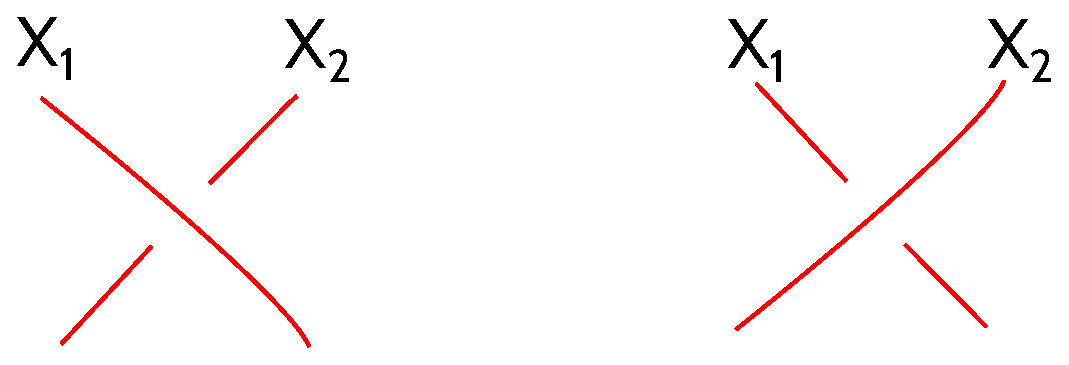
\includegraphics[width=0.4\textwidth]{braiding.eps}
\end{center}
\begin{Def}

A \textit{braided monoidal category} is a monoidal category with a braiding.

\end{Def}
\begin{Def}
A \textit{braided monoidal functor} $F:\C\ra\D$ is a monoidal functor which makes the following diagram commute for any $X, Y \in \C$.
\[
\xymatrix{FX \otimes FY \ar[r]^{\sigma'_{FX, FY}} \ar[d]_{J_{X, Y}} & FY \otimes FX \ar[d]^{J_{Y,X}}\\
F(X\otimes Y) \ar[r]^{F(\sigma_{X, Y})} & F(Y\otimes X)}
\]
\end{Def}

\begin{Expl}\rm
Before we come to the actual example, we will first introduce some classical terminology about finite groups.
\begin{Def}
For an abelian group $G$, a function $q:G\rightarrow \kk^\times$ is a \textit{quadratic form} if $q(g) = q(g\inv)$ and  for $g, g', h \in G$, the function \begin{equation}
	b(g, h) = \frac{q(gh)}{q(g)q(h)}
\end{equation} is symmetric, \begin{equation}
	b(g, h) = b(h, g),
\end{equation} and is a bicharacter, \begin{equation}
	b(gg', h) = b(g, h) b(g', h).
\end{equation}
\end{Def}
We call $q$ \textit{degenerate} if $b$ is degenerate. Picking a bicharacter $B$ on $G$, we can define the quadratic form \begin{equation}
	q(g) = B(g,g).
\end{equation}
\begin{Def}
A \textit{pre-metric group} is a pair $(G, q)$ where $G$ is an abelian group and $q$ is a quadratic form. A \textit{metric group} is a metric group with a non-degenerate quadratic form.	
\end{Def}
Now, let $\C$ be a pointed braided fusion category, the simple objects forming a group $G$ following section \ref{pfc}. For a simple object $X\in \OO(\C)$ of degree $g$, define the form $q(g) = \sigma_{X, X} \in \kk$, where $\sigma_{X, X}$ denotes the braiding of $X$ with itself. We have\begin{equation}
	q(gh) = q(g)q(h)b(g,h), g, h\in G
\end{equation}
where $b(g, h)  = \sigma_{Y, X} \circ \sigma_{X, Y}\in \Aut(X\ot Y) \in \kk^\times$ and $g$ and $h$ are the elements associated with the isomorphism classes of $X$ and $Y$ respectively. The fact that $b$ is a bicharacter is a direct consequence of the hexagon axiom (\ref{hex}), and hence $q$ is quadratic form. It can be shown that for any pre-metric group $(G, q)$, there exists a pointed braided fusion category $\C(G, q)$ that is unique upto braided equivalence. Further, it can also be shown that every pointed braided fusion category is equivalent to one of the form $\C(G, q)$. For details, we refer the reader to \cite[Section 8.4]{EGNO}.
\iffalse
One may similarly define a function $\omega: G\times G \times G \ra \kk^\times$ for the associativity morphism, and the pentagon axiom along with the two hexagon axioms yields a set of conditions on the functions $\omega$ and $\sigma$.
\begin{align*}
 	\omega(g_1g_2, g_3, g_4) \omega(g_1, g_2, g_3g_4) = \omega(g_1, g_2, g_3) \omega(g_1, g_2g_3, g_4) \omega(g_2, g_3, g_4)\\
 	\omega (g_2, g_3, g_1) \sigma(g_1, g_2g_3) \omega(g_1, g_2, g_3) = \sigma(g_1, g_3) \omega(g_2, g_1, g_3) \sigma(g_1, g_2)\\
 	\omega(g_3, g_1, g_2)\inv \sigma(g_1g_2, g_3) \omega(g_1, g_2, g_3) \inv = \sigma(g_1, g_3) \omega(g_1, g_3, g_2)\inv \sigma(g_2, g_3),
 \end{align*}for $g_1, g_2, g_3, g_4 \in G$. Couples $(\omega, \sigma)$ satisfying this condition form a group $Z_{ab}^3(G, \kk^\times)$. There is also a parametrization for isomorphism classes of braided functors between pointed braided fusion categories, as the group $B^3(G, \kk^\times)$. One can define the so-called \textit{abelian cohomology} of a group $G$ with coefficients in $\kk^\times$, for more details see \cite[Section 8.4]{EGNO}.
 \fi
\end{Expl}
\subsection{Modularity}
\begin{Def}\rm\label{twistdef}
 A \textit{ribbon structure} on a braided rigid monoidal category is a distinguished isomorphism for every object $X\in \C$,
\begin{align}
\theta_X: X \rightarrow X\nonumber
\end{align}
 such that for any objects $X,Y \in \C$, \begin{align}
\theta_{X\otimes Y} &= \sigma_{Y,X}\sigma_{X,Y}(\theta_X\otimes \theta_Y)\label{twist}\\
\theta_{X^*}&=\theta_X^*. \label{twistdual}
\end{align}
 \end{Def}
 A braided fusion category with a ribbon structure is called a \textit{ribbon} category.  The morphism $\theta$ is sometimes called the \textit{twist}. \\If $\C$ is a pivotal braided fusion category, then we automatically have a ribbon structure on $\C$ defined by \begin{equation}
 	 \theta_X = (\ev_X \otimes j_X)\circ(\id_{X^*} \otimes \sigma_{X^{**}, X})\circ(\coev_{X^*} \otimes \id_X),\label{thetax} 
 \end{equation}
 where $\coev_X:\mathbbm{1}\rightarrow X\otimes X^*$ and $\ev_X:X^*\otimes X\rightarrow \mathbbm{1}$ denote the rigidity maps. Graphically, the ribbon structure $\theta_X$ on $\C$ is denoted as follows.

\begin{center}
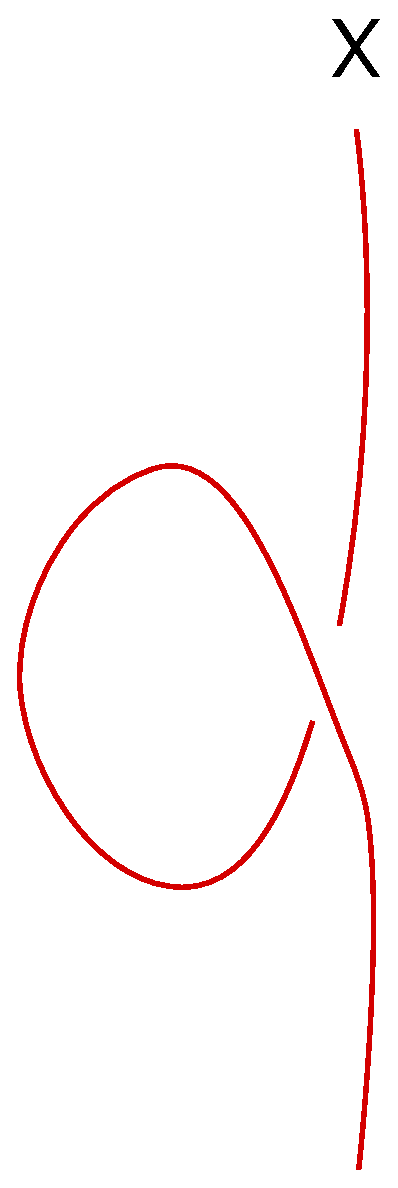
\includegraphics[width=0.1\textwidth]{t-matrix.eps}
\end{center}
\begin{defn}\label{mfcdef}\rm
A \textit{modular fusion category} $\Cat$ is a ribbon fusion category such that any simple object $X$ for which \begin{equation}\label{muger}
	\sigma_{Y,X}\sigma_{X,Y}= \id_{X\otimes Y}\end{equation}
 holds for every $Y\in \Cat$, is isomorphic to $\one$.
\end{defn}
The condition on $X$ in Definition \ref{mfcdef} is known as the \textit{non-degeneracy} condition.
 


\subsubsection{The Drinfeld center}
The Drinfeld center of a monoidal category $\C$, $\CTR(\C)$ is a construction which, starting from a monoidal category, yields a braided monoidal category. Let $\C$ be a monoidal category.
An object of $\CTR(\C)$ is the data $(X, \gamma_X)$, where $X\in \C$, and $\gamma$ is a functorial isomorphism \begin{equation}
	\gamma_X: X\otimes - \cong -\otimes X
\end{equation} such that the following diagram commutes. 
 \begin{align} 
\xymatrix { X\ot (Y \ot Z) \ar[r]^{a_{X, Y, Z}}\ar[d]^{\gamma_{Y\ot Z}} & (X\ot Y) \ot Z \ar[r]^{\gamma_Y\ot \id_Z} & (Y\ot X)\ot Z \ar[d]^{a_{Y, X, Z}} \\
(Y\ot Z)\ot X \ar[r]^{a\inv_{Y, Z, X}} & Y\ot (Z \ot X) & Y\ot (X \ot Z)\ar[l]^{Y\ot \gamma_Z}\\}
\end{align}
The morphism $\gamma$ is sometimes called the `half-braiding' (it being functorial in only one variable, as opposed to a braiding which is functorial in both variables).
The space of morphisms $\Hom_{\CTR(\C)}((X, \gamma_X), (X', \gamma_{X'}))$ consists of morphisms $f\in \Hom_\C(X, X')$ that are compatible with the half-braidings on $X$ and $X'$.
\begin{equation}
 	\xymatrix{X\otimes - \ar[r]^{\gamma_X} \ar[d]_{f\otimes \id_-} & - \otimes X \ar[d]^{\id_- \otimes f} \\
 	 	X'\otimes - \ar[r]^{\gamma_{X'}} &-\otimes X' }
 \end{equation}
 The tensor product of two objects, $(X, \gamma_X), (X', \gamma'_{X'})$, is the object $(X\otimes X', \gamma_{X\ot X'})$, $\gamma_{X\ot X'}$ being the half-braiding that makes the following diagram commute. \begin{equation}\label{halfbraidingcoherence}
 	 \xymatrix{(X\otimes X') \otimes Y \ar[r]^{a_{X, X', Y}} \ar[d]^{\sigma_{X\ot X', Y}} & X\otimes (X' \otimes Y)& X\otimes (Y \otimes X') \ar[l]_{\id_X \ot \sigma_{X', Y}} \\
 	  Y\otimes (X \otimes X') \ar[r]^{a_{Y, X, X'}} &  (Y\otimes X)\otimes X'\ar[r]^{\sigma_{Y, X}} & (X \otimes Y) \otimes X' \ar[u]^{a_{X, Y, X'}}  }
 \end{equation}
If $f:(X, \gamma_X)\rightarrow (X', \gamma_{X'})$ and $f': (Y, \gamma_Y) \rightarrow (Y', \gamma_{Y'})$ are two morphisms in $\CTR(\C)$, then $f\otimes f'$ is also a morphism in $\CTR(\C)$.

\iffalse If an object $Z\in \C$ has a left dual $Z^*$ then $(Z, \gamma)$ has a left dual $(Z^*, \gamma_{Z^*})$, with $\gamma_{Z^*}$ defined by the composition\begin{equation}
	\gamma_{Z^*}: Z^*\otimes - \xrightarrow{\id_{Z^*\otimes -} \otimes \coev_Z} Z^*\otimes - \otimes Z\otimes Z^* \xrightarrow{\id_{Z^*}\otimes \gamma_Z\inv \otimes \id_{Z^*}} Z^*\otimes Z \otimes - \otimes Z^*  \xrightarrow{\ev_Z \otimes \id_{-\otimes Z^*}} -\otimes Z^*,
\end{equation} 
a similar definition can be given for a right dual.\fi

There is an obvious forgetful functor $\CTR(\C)\rightarrow \C$, that forgets the half-braiding on each object,
\begin{equation}
	(X, \gamma)\mapsto X.
\end{equation}

\begin{Prop}
There is a canonical equivalence \begin{equation}
	\CTR(\C) \cong (\C\boxtimes \C^{op})^*_{\C} .
\end{equation}
\end{Prop}
\begin{proof}
A $\C$-bimodule endofunctor $F$ is in particular a left $\C$-module functor, and so $F= -\ot Z$ for some object $Z\in \C$. It is a right $\C$-module functor as well so we have a natural isomorphism \begin{equation}
	(X\ot Y) \ot Z = F(X\ot Y) \xra{s_{X, Y}} F(X) \ot Y = (X\ot Z)\ot Y,
\end{equation}
and the half-braiding associated with $Z$ may be defined as \begin{equation}
	 \gamma = s\inv_{\one, -}: Z \ot - \xra{\sim} -\ot Z.
\end{equation}
Consider the hexagon axiom for the module functor $F$
\[
\xymatrix{
X \ot (Y\ot Z) \ar[r]^{\id_X \ot s\inv_{\one, Y}} & X \ot (Z \ot Y)\ar[r]^{m_{X, Z, Y}} & (X\ot Z) \ot Y \ar[d]^{s\inv_{\one, X} \ot Y} \\
(X\ot Y )\ot Z \ar[u]^{m_{X, Y, Z}}& Z\ot (X\ot Y)\ar[l]_{s\inv_{\one, X\ot Y}} & (Z \ot X) \ot Y. \ar[l]_{m_{Z, X, Y}}  \\   
}
\]
The two arrows on top compose to give the morphism $s_{X, Y}$, which turns the above diagram into a pentagon, and it is easily seen that this is the pentagon axiom for the right $\C$-module category $\C$. Thus the hexagon condition is satisfied for our definition of $\gamma$.
For bimodule endofunctors $F$ and $G$, let $F= -\ot Z$ and $G = -\ot W$ for object $W, Z \in \C$, then the composition \begin{equation}
	GF(X\ot Y) \xra{\sim} G(F(X)\ot Y) \xra{\sim}GF(X) \ot Y
\end{equation} yields the braiding associated with the object $Z\ot W$ and so the functor $G\circ F$ is given by the tensor product of the corresponding objects in the center.\\
 In the other direction, starting from objects $(W, \gamma_W)$ and $(Z, \gamma_Z)$ for $W, Z \in \C$, we can define functors $F:= -\ot Z$ and $G:= -\ot W$, and use the half-braidings and their properties to show that these indeed define $\C$-bimodule endofunctors.
\end{proof}

\begin{Prop}\label{centereqv}
The category $(\C\boxtimes \C^*_\M)^*_\M$ is tensor equivalent to $\CTR(\C)$.
\end{Prop}
\begin{proof}
An object of $(\C\boxtimes \C^*_\M)^*_\M$ is a $\C\boxtimes \C^*_\M$-module endofunctor of $\M$, and in particular it is a $\C^*_\M$-module endofunctor, which by Theorem \ref{can} is isomorphic to one of the form $Z\ot -$ for some object $Z\in \C$. We then have an isomorphism for \begin{equation}
	X\ot F(Z\ot -) \cong Z\ot(X\ot F(-)),\label{moduleiso}
\end{equation}for $F\in \C^*_M$ and $X \in \C$, which is the $\C \boxtimes \C^*_\M$ module functor structure. If we let $F=\id$, then we get an isomorphism of $\C^*_\M$-module functors \begin{equation}
	X\ot Z \ot -\xra{\sim} Z\ot X\ot -.
\end{equation}
By the equivalence \ref{can}, $X\mapsto X\ot -$ for $X\in \C$, we get a natural isomorphism $\gamma_X: X\ot Z \ra Z \ot X$. The coherence diagram for the module functor $F$ translates \eqref{moduleiso} into the coherence diagram \eqref{halfbraidingcoherence}, and thus we have that  $(Z, \gamma)$ is an object of $\CTR(\C)$. In the other direction, given an object $(Z, \gamma) \in \CTR(\C)$ , there is a structure of a $\C\boxtimes \C^*_\M$-module functor on $Z\ot -$ by virtue of the half-braiding $\gamma$. It is clear that the two assignments above are tensor quasi-inverses of each other.
\end{proof}
\begin{Prop}
For $\C$ a fusion category, there is a tensor equivalence \begin{equation}
	\CTR(\C)\cong \CTR(\C^*_\M).
\end{equation}
\begin{proof}
In the statement of Proposition \ref{centereqv}, if we substitute $\C$ by $\C^*_\M$, then we get 
\begin{equation}
	(\C^*_\M \boxtimes (\C^*_\M)^*_\M)^*_\M \cong \CTR(\C^*_\M),
\end{equation} but using Proposition \ref{can} we can write \begin{equation}
	(\C^*_\M \boxtimes \C)^*_\M \cong \CTR(\C^*_\M)
\end{equation} but the left hand side is equivalent to $\CTR(\C)$ so the claim follows.
\end{proof}
\end{Prop}

Let $\C$ be a modular fusion category. The non-degeneracy condition in Definition \ref{mfcdef} can be expressed as the non-degeneracy of the symmetric matrix $S$, 
\begin{equation}\label{S}
	S: S_{XY}= \text{tr}(\sigma_{Y,X^*}\circ\sigma_{X^*,Y}),
\end{equation}
where \begin{align}
	\text{tr}(\sigma_{Y,X^*}\circ\sigma_{X^*,Y}) = ((\ev_{X^*}\otimes \ev_{Y^*}) \circ (j_{X}\circ\id_{X^*} \otimes j_Y \otimes \id_{Y^*}))\circ\\ (\id_X\otimes (\sigma_{Y,X^*}\circ\sigma_{X^*, Y}) \otimes \id_{Y^*})\circ (\coev_X \otimes \coev_Y) \label{Strace}
\end{align}

for $X,Y \in \mathcal{\OO(\Cat)}$, where tr denotes the quantum trace. Graphically this is represented as the closure of a double braiding, as follows.
\begin{center}
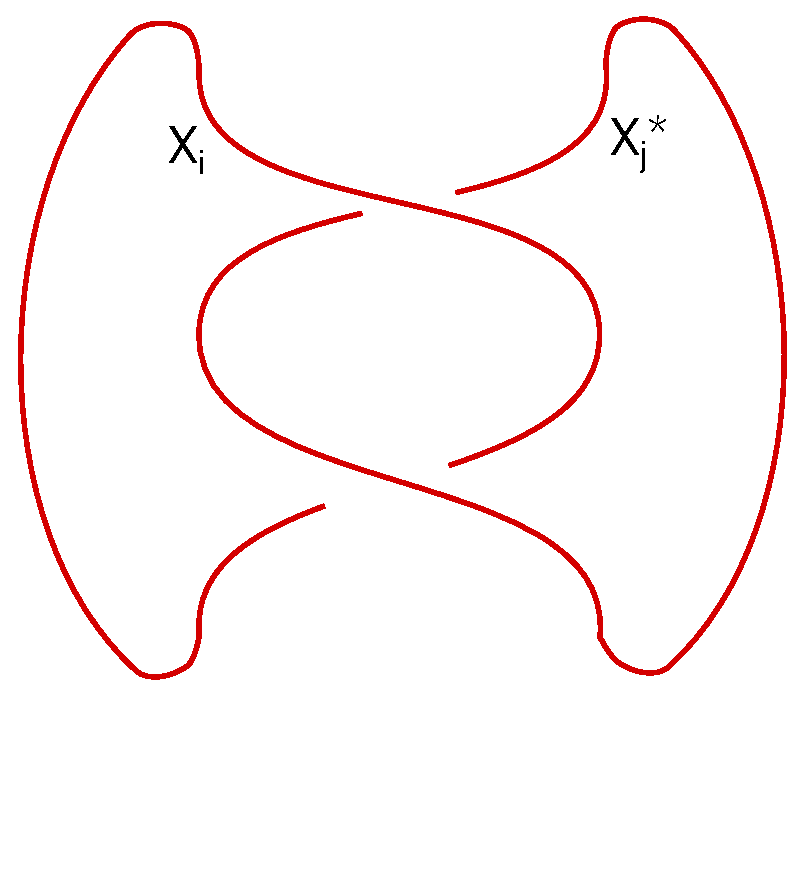
\includegraphics[width=0.2\textwidth]{s-matrix.eps}
\end{center}
For a simple object $X_i$ ($i\in \mathcal{I}$), the morphism $\theta$ (see \ref{twistdef}) is a scalar matrix $\omega_i \id_{X_i}$. The diagonal matrix $T$ is defined as 

\begin{equation}\label{T}
	T: T_{ii} = \omega_i.
\end{equation}
By Vafa's theorem (see\cite[Theorem 3.1.19]{BK}), the $T$-matrix has finite order, so the $\omega_i$'s are roots of unity. The order of the $T$-matrix is called the \textit{exponent} of the MFC.\\
The data of the $S$-matrix and $T$-matrix is together called the \textit{modular data}. It gives rise to a projective representation of the modular group $\text{SL}_2(\Z)$ which is also the mapping class group of the torus. While the $S$ and $T$ matrices provide a lot of information about the MFC they arise from (for instance, they completely determine the fusion ring), they do not serve as complete invariants for MFCs, i.e., two MFCs that are non-equivalent as braided tensor categories may give rise to the same modular data \cite{2017arXiv170802796M}.


\chapter{A topological invariant for modular fusion categories}\label{chp3}
The modular data of a modular category $\C$ comprises the $S$- and $T$-matrices, two square matrices indexed by the isomorphism classes of simples; they define a projective representation of the modular group. The importance of the modular data has led to the question being seriously considered (and stated as not quite a conjecture in \cite{BNRW}) as to whether a modular category (and hence the TQFT associated to it) is already determined fully by the modular data. This was refuted in \cite{2017arXiv170802796M} by a family of examples that are the Drinfeld centers of pointed fusion categories, which were already considered, in the guise of representation categories of twisted Drinfeld doubles of finite groups, in \cite{DijPasRoc:QHAGCOM}. It turns out in fact that arbitrarily many inequivalent modular categories can give rise to the same modular data; the examples are defined by the same noncommutative group, endowed with different three-cocycles; the smallest example in \cite{2017arXiv170802796M} concerns the nonabelian group of order $55$.

This result naturally gives rise to the following question: Can one find other invariants that distinguish the modular categories in these families? 

The simple idea of this chapter is to consider the invariant of a certain framed link defined by the modular categories in question and view it as an invariant of the category, much like the invariant of the Hopf link giving the $S$-matrix. The particular link we will use is known as the borromean rings. This is partly an obvious candidate for naive reasons: It is the closure of a three-strand braid, which is the next more complicated thing over the two-strand braid whose closure is the Hopf link; having three strands might allow the associativity constraint of the category (which, after all, is encoded in the three-cocycle that makes the basic difference in the aforementioned examples)  to have a greater influence on the invariant. Since the invariant obtained from a full twist on three strands (like the Hopf link comes from a full twist on two strands) is determined by the modular data, making inverse braidings appear seems necessary, and the braid whose closure gives the borromean rings does this in a somewhat symmetric fashion. It may also be a good candidate for a slightly less naive reason: The borromean rings are three circles that are pairwise not linked, yet form a nontrivial link. This is a somewhat subtle topological phenomenon which one may hope gives rise to an invariant whose properties are \emph{not} covered by those of the $S$-matrix, which records precisely what happens if two rings are linked. (In fact, the rings seem to have appeared in 15th century Italy as a heraldic symbol for this very reason: They are supposed to symbolize the political (and marital) alliances between the Borromeo, Sforza, and Visconti families, which was such that removing any one of them would have broken the alliance of the three.) Whether the motivations are justified by the success is perhaps doubtful: The borromean tensor does not at all distinguish the categories described above. In fact it does not seem to ``see'' the three-cocycle at all that makes the difference between the categories. It is only the $T$-matrix taken together with the $B$-tensor that makes it impossible to find a bijection between the simples of the different categories that would map these data to each other.

The same general idea of using link invariants to distinguish modular categories not distinguished by modular data was also pursued in \cite{2018arXiv180505736B}, where the authors show that the invariant of the Whitehead link, along with the $T$-matrix, does distinguish the five inequivalent modular categories defined from the nonabelian group of order $55$. We are grateful to the authors for letting us see an advance copy of their preprint. At the time we knew by computer experiments that the invariant of the borromean rings, taken together with the modular data, also distinguishes the categories in this particular example, and we knew which components of the ``borromean tensor'' (given by the invariants of the borromean link with its three components colored by three simples of the category) are responsible for this success. We had not finished writing our findings, and we had not completed the results in \cref{sec:Example} showing that the $T$-matrix together with the borromean tensor is sufficient to distinguish the modular categories associated to the nonabelian groups of order $pq$ (for all primes $p,q$ for which such a group exists).

This chapter is organized as follows: After introducing conventions and notations, we first revisit the modular data of twisted Drinfeld doubles to give a slightly improved formula for the $S$-matrix, but mostly to introduce the methods to be used later. We formally define the Borromean tensor in \cref{sec:borromean-tensor} and record some symmetry properties it enjoys. In \cref{sec:borr-tens-twist} we give an explicit formula for the Borromean tensor for twisted Drinfeld doubles, with some useful specializations that we then use in \cref{sec:Example} to explicitly distinguish the inequivalent modular categories found in \cite{2017arXiv170802796M} by the new numerical invariant that is the $B$-tensor together with the $T$-matrix. We then study twisted doubles for square-free groups in \cref{sub:twisted_doubles_of_square-free groups}, and then in \cref{squarefreeS} study how much information the S-matrix can deduce for such modular fusion categories. Finally in \cref{squarefreeB} we show that the $B$-tensor together with the $T$-matrix serves as a complete invariant for twisted doubles of square-free groups. An appendix gives some GAP codes for computing the $B$-tensor (and the $S$-matrix). Experimenting with computer calculation was an important step in our work, although computer help is not needed to prove the main result; some calculations were performed using HPC resources from PSIUN CCUB (Centre de Calcul de
l'Université de Bourgogne).
\section{Twisted doubles of finite groups: structure and modular data}
One \emph{raison d'être} of modular categories is that they allow the definition of a topological quantum field theory. In particular they define invariants in $\CC$ of framed knots and links. We will freely use graphical notation for morphisms in a modular category $\C$, recalled in Chapter 2. The framed link invariant defined by a modular category can be viewed as follows: The link is the closure of a braid. The braid in question, colored by objects in $\C$,  defines an endomorphism of a tensor product of o{}bjects in $\C$, and taking the closure of the braid corresponds to taking the (pivotal) trace of the endomorphism. To fix notations regarding this procedure, there is a representation of the braid group on $n$ strands
$$R\colon\mathbb B_n\to\operatorname{Aut}_{\C}\bigl( (\dots(V\ot V)\ot V)\ot V)\dots \ot V)\bigr)$$
on the tensor product of $n$ copies of any object $V\in\C$. In the case of a non-strict category (as indicated by the parentheses) this involves both instances of the braiding $\sigma$, and instances of the associator isomorphism $\Phi$. We will also need to consider analogous morphisms defined on tensor products of distinct objects; informally we will write
\begin{multline*}
  R(\beta)\colon (\dots((V_1\ot V_2)\ot V_3)\dots\ot V_n)\rightarrow (\dots((V_{\beta\inv(1)}\ot V_{\beta\inv(2)})\ot V_{\beta\inv(3)})\dots\ot V_{\beta\inv(n)}) 
\end{multline*}
for $\beta\in\mathbb B_n$ and $V_1,\dots,V_n\in\C$, where $\beta$ also denotes the underlying permutation of $\beta$. We note that  $R(\beta\beta')=R(\beta)R(\beta')$ in the obvious sense for two braids $\beta,\beta'$.

 We need to fix notations and collect a few useful identities. We will denote by $(X_i)_{i\in I}$ a set of representatives of the isomorphism classes of simple objects of $\C$, and write $i^*\in I$ for the element such that $X_{i^*}=X_i^*$ is the dual object. We will denote the pivotal trace in the category $\C$ of an endomorphism $f$ by $\ptr(f)$. We will write $g\hit h=ghg\inv$ for the action of a group on itself by conjugation, $C_G(g)$ for the centralizer of $g$ in $G$, and $g^G$ or $\ol g$ for the conjugacy class of $g\in G$. 
Let $|u|$ denote the degree of the homogeneous element $u$, and $\omega\colon G^3\rightarrow\CCu$ a three-cocycle. In the sequel, we will always tacitly assume that elements of graded vector spaces are homogeneous in writing such formulas.

We will not explicitly need the pivotal structure of $\Vect^\omega_G$ but only the fact that pivotal traces of endomorphisms are simply the usual traces of the underlying linear maps.

We now describe the structure of the Drinfeld center of $\Vect^\omega_G$, $\mathcal{Z}(\Vect^\omega_G)$. The structure of an object $(W,\sigma_{\cdot,W})$ in the center, with $\sigma_{V,W}\colon V\ot W\to W\ot V$ the half-braiding for $V\in\Vect_G^\omega$ can be described in terms of an action (not quite a group action) of $G$ on $W$ \cite{Maj:QDQHA}. More precisely, giving a half-braiding is equivalent to giving a map
$\hit\colon G\otimes W\to W$ subject to the conditions
\begin{align}
  |g\hit w|&=g\hit|w|\\
  e\hit w&=w\\
  g\hit h\hit w&=\alpha_{|w|}(g, h)gh\hit w
\end{align}
for $g,h\in G$ and $w\in W$, and $|\cdot|$ denotes the degree of the element $\cdot$. The braiding isomorphism is described by the formula
\begin{equation*}
  V\ot W\ni v\ot w\mapsto |v|\hit w\ot v\in W\ot V.
\end{equation*}

Let $V\in\CTR(\Vect_G^\omega)$. Since acting by an element $g\in G$ is a vector space automorphism of $V\in\Vect_G^\omega$ which conjugates degrees, any object decomposes as the direct sum of objects where the degrees of nonzero homogeneous components form a conjugacy class. Assume that the degrees of the nonzero components of $V$ form a conjugacy class. Then $G$ permutes those homogeneous components transitively, and elements in the centralizer $C_G(g)$ map the homogeneous component $V_g$ to itself. In particular, $V_g$ is an $\alpha_g$-projective representation of $C_G(g)$ where
\begin{equation}\label{alpha}
\alpha_g(x,y)=\omega(x,y,g)\omega^{-1}(x,y \hit g,y)\omega(xy \hit g ,x ,y)
\end{equation}
and the structure of $V$ is determined by this projective representation for any one $g$ in the conjugacy class. In particular, simple objects of $\CTR(\Vect_G^\omega)$ are parametrized by pairs $(g,\chi)$ where $g$ runs through a system of representatives for the conjugacy classes of $G$, and $\chi$ is an irreducible $\alpha_g$-projective character of $C_G(g)$.

It is convenient to note, for later, how to obtain the $C_G(x)$-projective character $\chi'$ describing the action of $C_G(x)$ on $V_x$ when $x$ belongs to the same conjugacy class, say $x=f\hit g$. So let $c\in C_G(x)$ and $v\in V_g$. We have

\begin{align}\label{1}
c \hit (f \hit v) &= \alpha_{g}(c, f) cf \hit v\\
f \hit ((f\inv\hit c) \hit v)   &= \alpha_{g}(f, f^{-1}\hit c) cf \hit v
\end{align}
and therefore
\begin{equation*}
  c\hit f\hit v  = \alpha_{g}(c, f) \alpha_{g}\inv(f, f^{-1}\hit c) f \hit (f\inv\hit c)\hit v .
\end{equation*}
This means that the diagram
\begin{equation*}
\xymatrix {V_g \ar[rr]^{f\hit} \ar[dd]_{(f^{-1} \hit c)\hit}   & & V_x \ar[dd]^{c\hit}\\
\\
 V_g \ar[rr]^{f\hit}  & & V_x}
\end{equation*}
commutes up to the scalar factor $\alpha_{g}(c, f) \alpha_{g}\inv(f, f^{-1}\hit c)$. By cyclicity of the trace, the projective character of the projective $C_G(x)$-representation $V_x$ is therefore $\chi^x$, given by
\begin{equation}\label{chi}
  \chi^x(c) :=(f\hit\chi)(c):=\alpha_{g}(c, f) \alpha_{g}\inv(f, f^{-1}\hit c)\chi(f\inv\hit c).
\end{equation}
In particular this expression does define a projective character, and does not depend on the choice of $f\in G$ with $f\hit g=x$.

The inverse of the braiding in $\CTR(\Vect_G^\omega)$ is given by $\sigma\inv(w\ot v)=v\ot |v|\inv\bhit w$, where $\bhit\colon\CC G\otimes V\to V$ is such that $g\hit g\inv\bhit v=g\inv\bhit g\hit v=v$. From
\begin{align*}
  f\inv \hit (f \hit v) &= \alpha_{|v|}(f\inv, f) v,\\
  f\hit f\inv\hit v&=\alpha_{|v|}(f,f\inv)v
\end{align*}
one reads off
\begin{align}\label{blackhit}
f\inv\bhit v&=\alpha_{|v|}\inv(f,f\inv) f\inv\hit v,\\
  f\inv\bhit v&=\alpha_{f\hit|v|}\inv(f\inv,f) f\inv\hit v,
\end{align}
respectively.

It is of course well-known how to compute the modular data of the twisted Drinfeld double of a finite group \cite{MR1770077}. In particular the $T$-matrix is given by
\begin{equation}
  \label{eq:tmatrix}
  T_{(g,\chi)}=\Theta(g,\chi)=\frac{\chi(g)}{\chi(1)}.
\end{equation}
We will rederive a formula for the $S$-matrix with only a slight advantage: The formula from \cite{MR1770077} involves a double sum, over two conjugacy classes, or twice over the group. Our formula has only one sum. Recall from \cite{MR1770077}, that the $S$-matrix is the trace of a braid on two strands (whence the two sums, related to the two objects coloring the strands); generally, the invariant obtained from taking the trace of a braid on $n$ strands would involve $n$ summations, over the conjugacy classes associated to the objects, but one can get away with only $n-1$ summations by a simple trick based on a well-known fact.

In the graphical calculus, taking the trace of the image of a braid in a pivotal monoidal category amounts to closing the braid. Obviously, one can choose to close all strands but one, which leaves us with an endomorphism with the object labelling the remaining strand, and then take the trace of that endomorphism. More formally:
\begin{Rem}\label{pretrick}\rm
  Let $V,W\in\C$ and $f\colon V\ot W\to V\ot W$. Then
  $\tr(f)=\tr(\ptr_V(f))$, where
\begin{center}
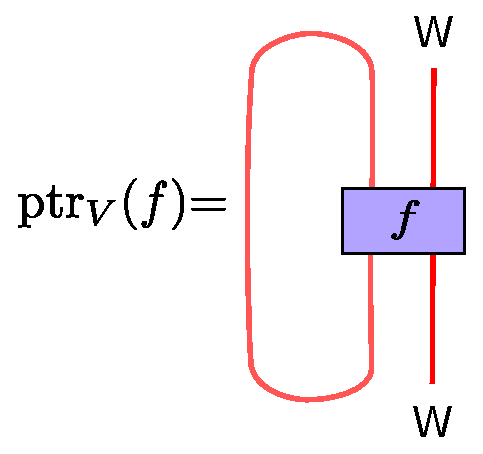
\includegraphics[width=0.25\textwidth]{ptr.eps}
\end{center}
  is a partial (pivotal) trace. If $W$ is simple, then $\ptr_V(f)=\lambda\cdot\id_W$ is a scalar, and $\tr(f)=\lambda\dim(W)$.
\end{Rem}

Working in the category $\CTR(\Vect_G^\omega)$, where formulas for the traces of braids involve sums over all the combinations of $G$-degrees of each object (subject to some condition), this will allow us to get away with one less sum (or, when coding the formulas, one less nested loop):
\begin{Rem}\label{trick}\rm
  Let $V,W\in\CTR(\Vect_G^\omega)$ with $W$ the simple object corresponding to $(g,\chi)$, and let $f\colon V\ot W\to V\ot W$. Then $\ptr_V(f)=\lambda\id$; the scalar $\lambda$ is determined by the component $\ptr_V(f)|_{W_g}\colon W_g\to W_g$ of $\ptr_V(f)$ by $\lambda\dim W_g=\tr(\ptr_V(f)|_{W_g})$, and thus $\tr(f)=|\overline g|\tr(\tr_V(f)|_{W_g})$
\end{Rem}

As an illustration and warm-up for the calculations in \cref{sec:borr-tens-twist} we will consider the $S$-matrix for two simple objects $V,W\in\mathcal{Z}(\Vect^\omega_G)$, corresponding to the pairs $(g,\chi_1)$ and $(h, \chi_2)$. We need to compute
\begin{equation*}
  S_{(g,\chi_1),(h,\chi_2)}=\tr(\sigma_{WV}\sigma_{VW})=\tr(\sigma^2)=\tr(R(\sigma^2)),
\end{equation*}
where (no parentheses being necessary on two objects) there is no difference between the representation $R$ of the braid group $\mathbb B_2$ on one generator $\sigma$ and simply instances of the braiding of the category $\CTR(\Vect_G^\omega)$.

If we write $V = \underset{x\in \overline{g}}\oplus V_x$ and $W = \underset{x\in \overline{h}}\oplus W_y$, then for $  v\in V_x$ and $  w\in W_y$ we have
\begin{align*}
  \sigma^2(  v\ot  w)&=\sigma(x\hit   w\ot   v)\\
  &=|x {\hit}  w|\hit   v\ot x\hit   w\\
  &=(x\hit y) \hit   v\ot x\hit  w.
\end{align*}

We can endow $V\ot W$ with a $G\times G$-grading composed of the $G$-gradings of $V$ and $W$. Then
\begin{align*}
  \deg_{G\times G}\sigma^2(v\ot w)=((x\hit y) \hit x,x \hit y)
\end{align*}
for $x=|v|,y=|w|$.

For a finite group $\Gamma$, a $\Gamma$-graded vector space $E$, and an endomorphism $f$ of $E$ let $f_0$ be trivial component of $f$ with respect to the $\Gamma$-grading of $\End(E)$. Then $\tr(f)=\tr(f_0)$.

In our example, considering the $G\times G$-grading of $V\ot W$, we see that $\sigma^2( v\ot  w)$ has the same degree as $v\ot w$ if and only if $x$ and $y$ commute.

\begin{equation} \label{degree condition}
(\sigma^2)_0(v\ot w) = \begin{cases} 
          x\hit v\ot y\hit  w & [x,y]=1 \\
          0 & [x,y] \neq 1 
       \end{cases}
\end{equation}

In particular
\begin{equation*}
  S_{V,W}=\tr(\sigma^2)=\tr((\sigma^2)_0)=\sum_{\substack{x\in \overline g\\y\in\overline h\\ [x,y]=e}}\chi_1^x(y)\chi_2^y(x)
\end{equation*}
Using \cref{trick} we can replace the double sum by a single sum; also, we can use~(\cref{chi}):
\begin{align*}
S_{(g, \chi_1),(h, \chi_2)} &= |\hb|\sum_{x \in \gb}^{[x,h]=1} \chi_1^x (h) \chi_2 (x)\notag\\
%\label{Sconj}
&=|\hb| \sum_{x \in \gb}^{[x,h]=1} \alpha_{g}(c, p) \alpha_{g}\inv(p, p\inv\hit c)\chi_1(p\inv\hit c) \chi_2 (x)
\end{align*} 
where $p$ stands for any group element satisfying $p\hit g=x$. Alternatively, we can use the bijection $G/C_G(g) \rightarrow g^G$ given by $aC_G(g)\mapsto a\hit g $ to rewrite
\begin{align*}\label{Sgroup}
  S_{(g, \chi_1),(h, \chi_2)} &=\frac{|\hb|}{|C_G(g)|}\sum^{[p\hit g,h]=1}_{p\in G} \alpha_{g}(h, p) \alpha^{-1}_{g}(p, p^{-1}\hit b)\chi_1(p^{-1}\hit b) \chi_2 (p\hit g)\\
  &={|\hb|}\sum^{[p\hit g,h]=1}_{p\in G/C_G(g)} \alpha_{g}(h, p) \alpha^{-1}_{g}(p, p^{-1}\hit b)\chi_1(p^{-1}\hit b) \chi_2 (p\hit g)
\end{align*}
As mentioned, this formula is (up to conventions) quite like the formula in \cite{MR1770077}, except for two details: We have a single sum over one conjugacy class instead of a double sum, and we have half the cocycle (``$\alpha$'') terms due to the fact that we need to use (\cref{chi}) on only one of the two objects.

\section{The B-tensor}\label{sec:borromean-tensor}

A modular category (in fact any spherical braided fusion category) defines a numerical invariant of framed knots and links which can be written as the pivotal trace of the image in the category of a braid whose closure is the link, with its components colored by simple objects of the category. Read differently, each fixed framed link defines a numerical invariant of modular categories in this fashion. More precisely, the invariant is then indexed by as many simple objects as the link has components.

Among this infinite supply of numerical invariants (among which the $S$-matrix and, up to a dimension factor, the $T$-matrix can also be found) we pick one example, for the heuristic (and art historical) reasons cited at the beginning of this chapter.

\begin{Def}
  The borromean tensor (or $B$-tensor) of a modular category $\C$ with simples $(X_i)_{i\in I}$ is the family
  \begin{equation}
    \label{eq:borromeo}
    B_{ijk}:=\tr(B((\sigma_2\inv\sigma_1)^3)
  \end{equation}
  where $B((\sigma_2\inv\sigma_1)^3)\in\Aut_{\C}((X_i\ot X_j)\ot X_k)$. Graphically, this may be represented as 
\begin{center}
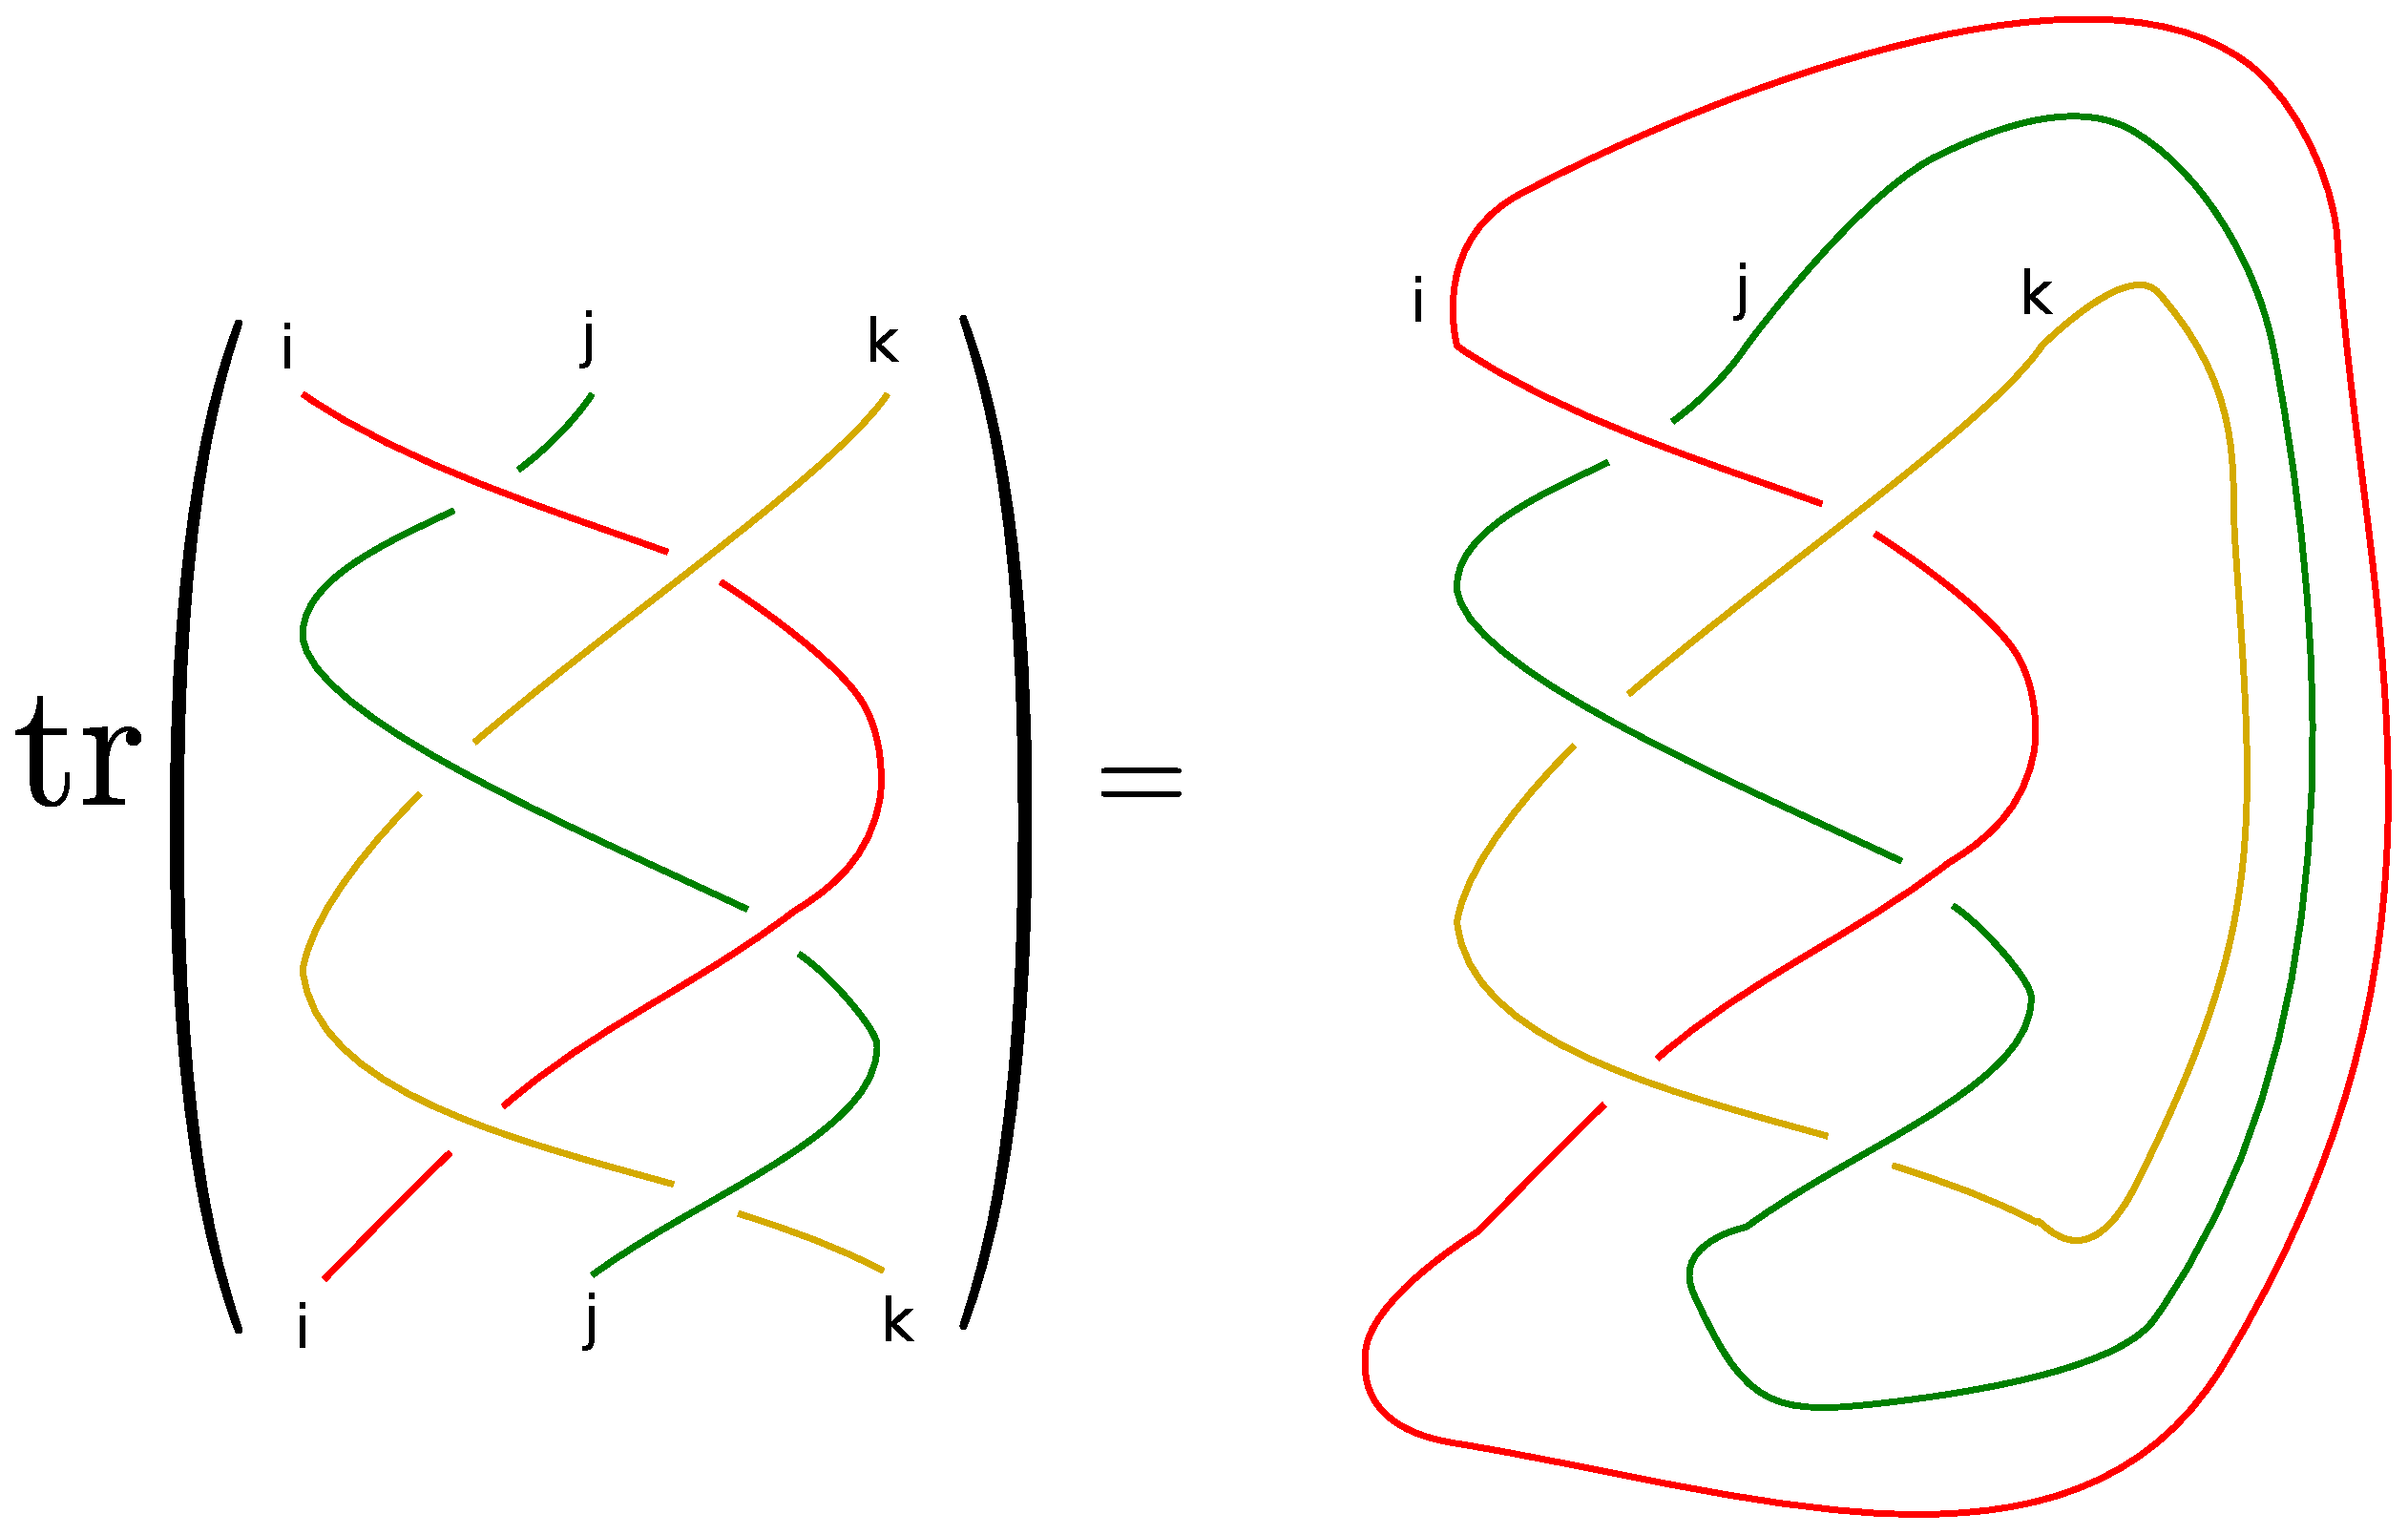
\includegraphics[width=0.5\textwidth]{b-braid.eps}
\end{center}
or more symmetrically, 

\begin{center}
\includegraphics[width=0.4\textwidth]{b-tensorc2.eps}
\end{center}

(In the graphical representation, we let $i$ stand for $X_i$.)
\end{Def}
\begin{Lem}
 The following equalities hold:
\begin{enumerate}
\item
$B_{ijk}=B_{jki}=B_{kij}$
\item
$B_{ijk}=B_{jik^{\ast}}$
\item
$B_{ijk}=\overline{B_{kji}}$ if $\C$ statisfies the $\mathcal F$-property (see \cite{MR2832261}).
\end{enumerate}
\end{Lem}
\begin{proof}
Clearly cyclicity of the trace implies that the $B$-tensor is invariant with respect to cyclic permutations of its three indices. We need to show the other symmetry properties:
If we conjugate the braid corresponding to the $B$-tensor by
\begin{center}
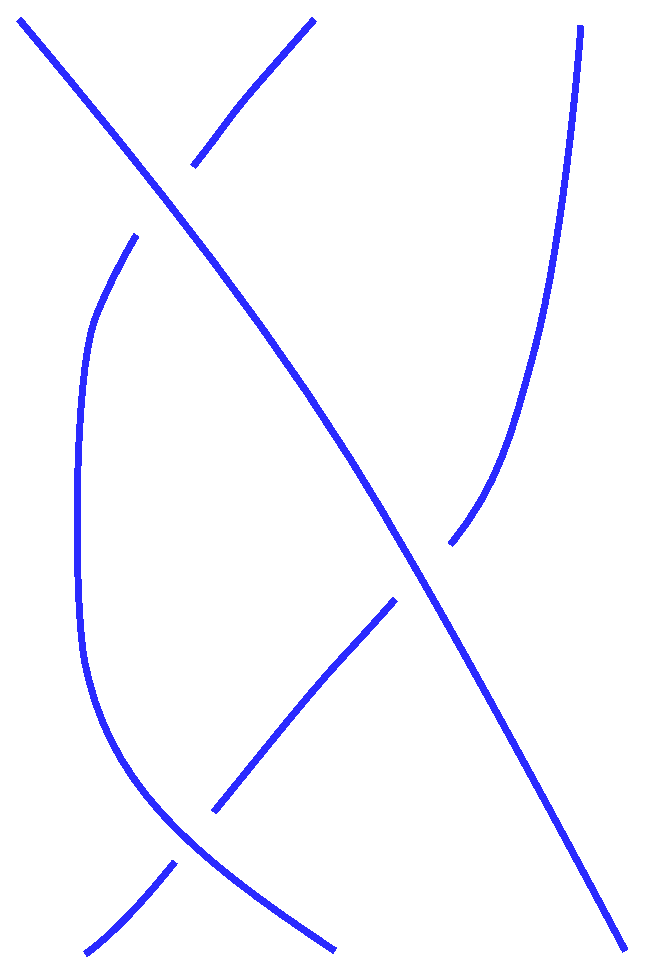
\includegraphics[width=0.08\textwidth]{conj.eps}
\end{center}
then we get that the trace of the resulting braid, 
\begin{equation}\label{conjugated}
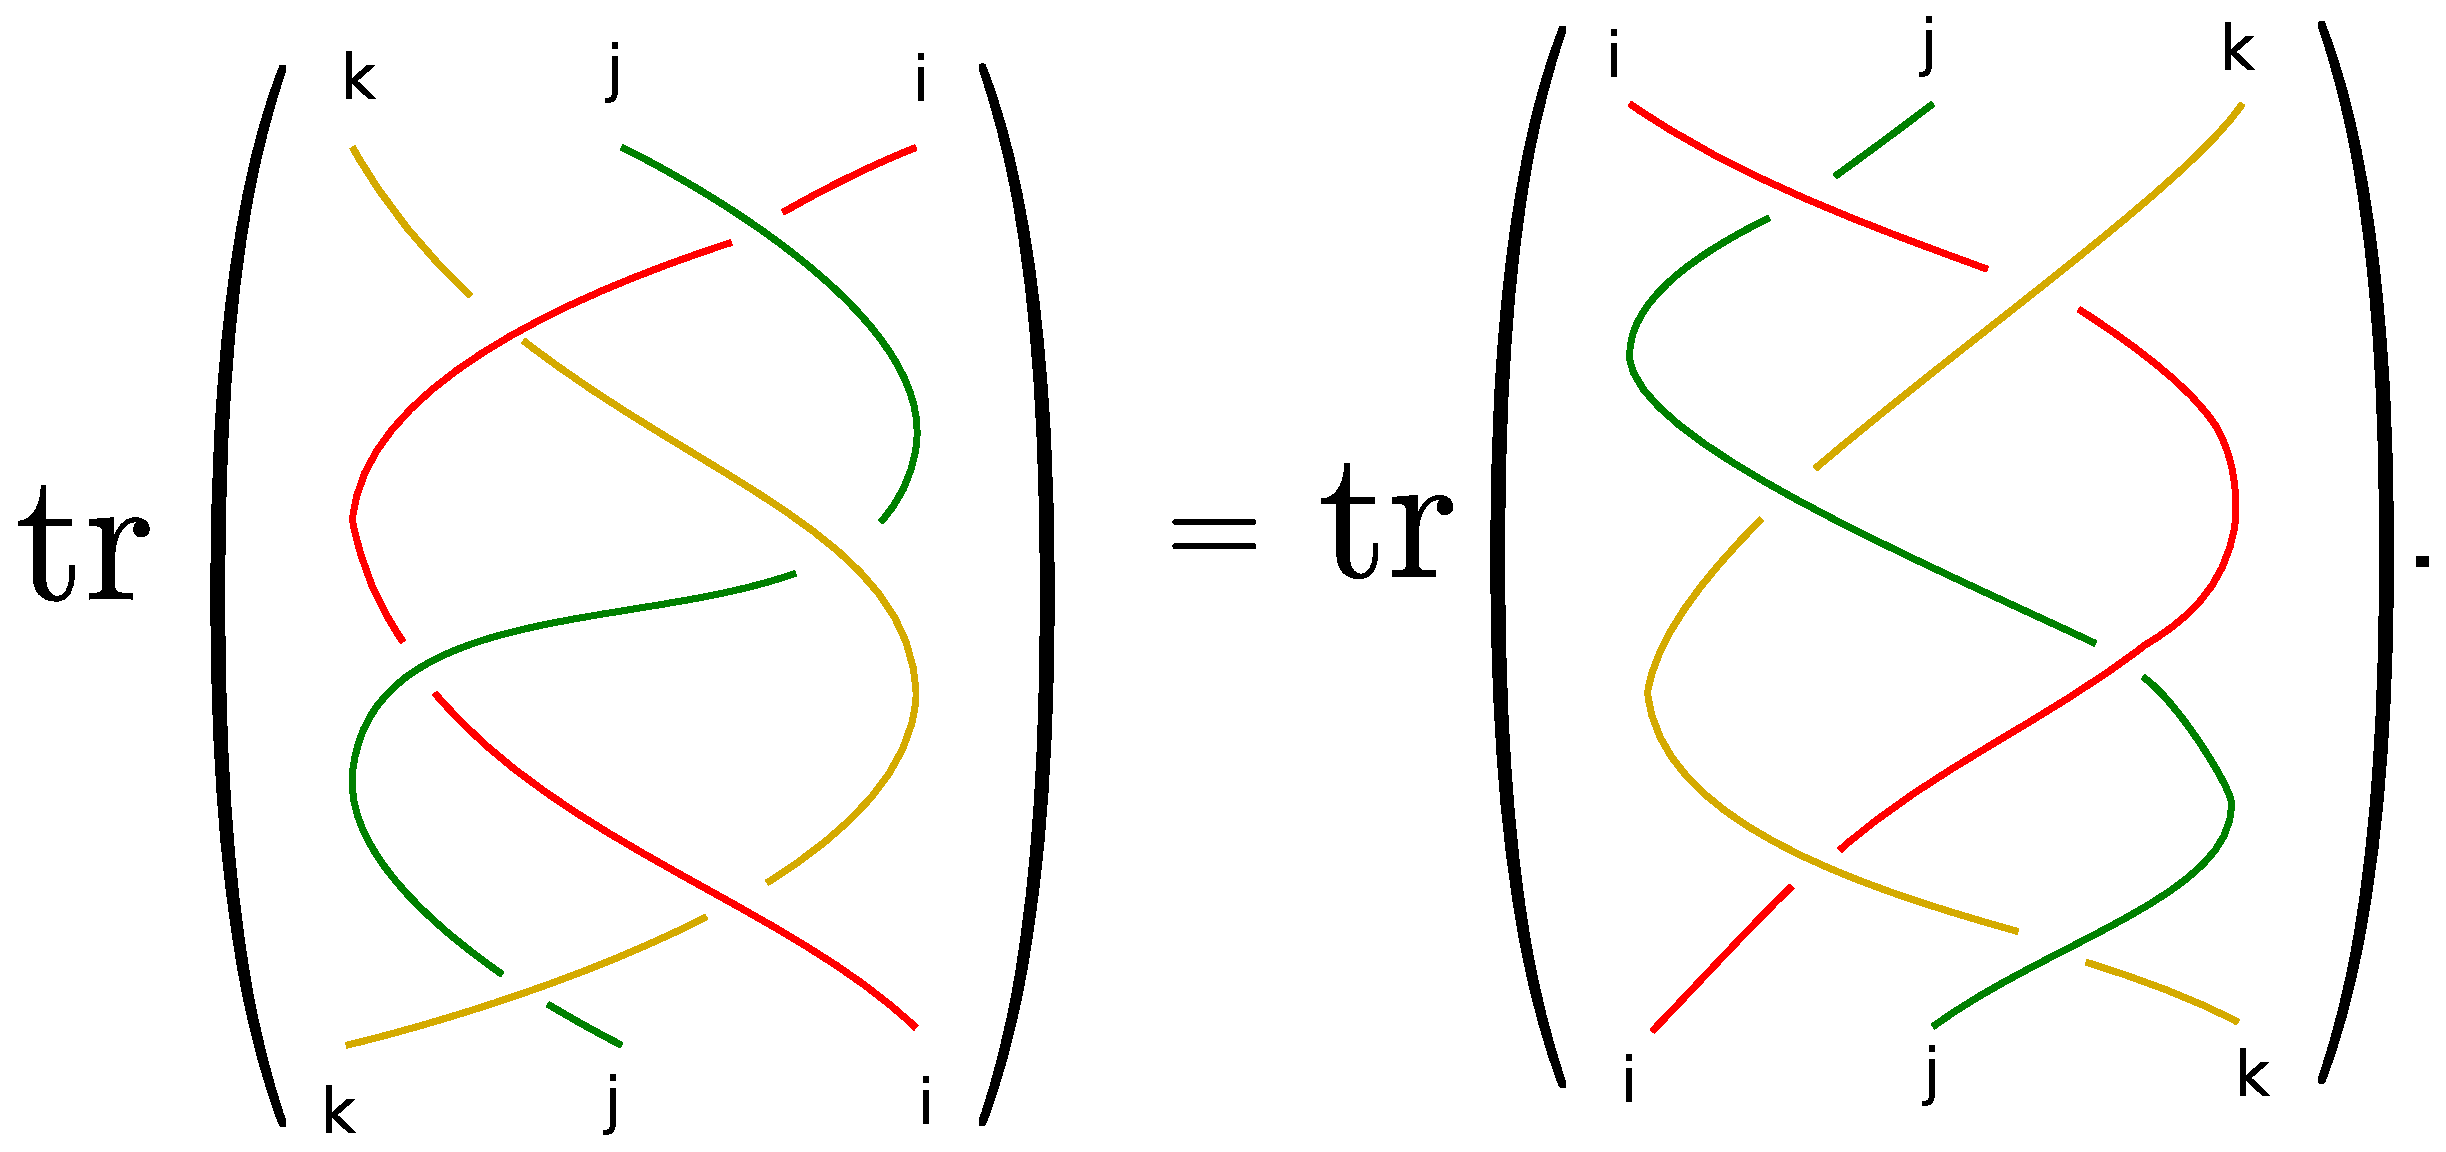
\includegraphics[width=0.5\textwidth]{conjugated.eps}
\end{equation}
 
Furthermore, we have
\begin{equation*}
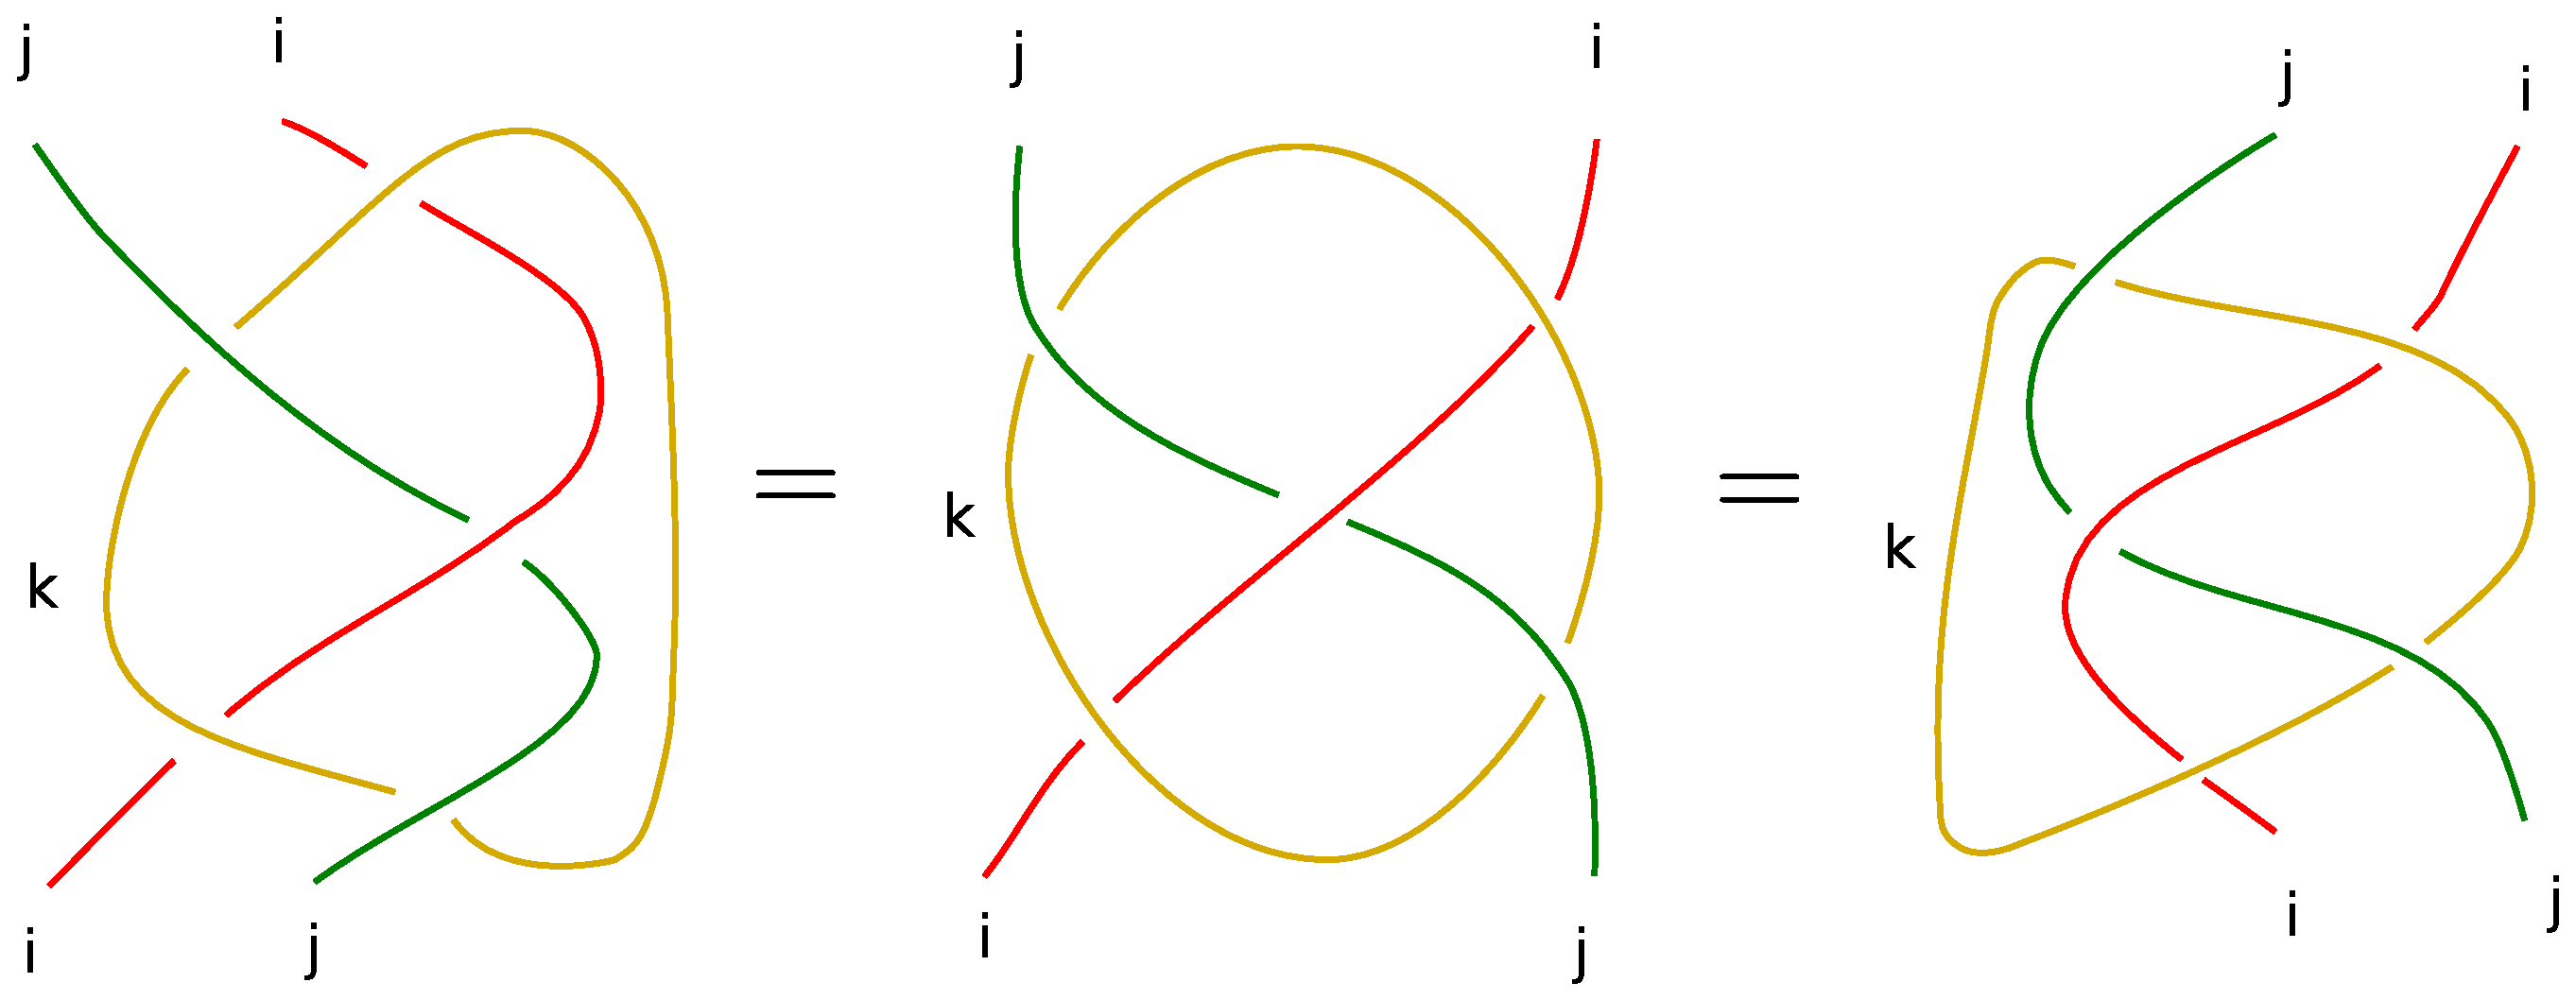
\includegraphics[width=0.7\textwidth]{slidethru.eps}
\end{equation*}
and thus,
\begin{equation*}
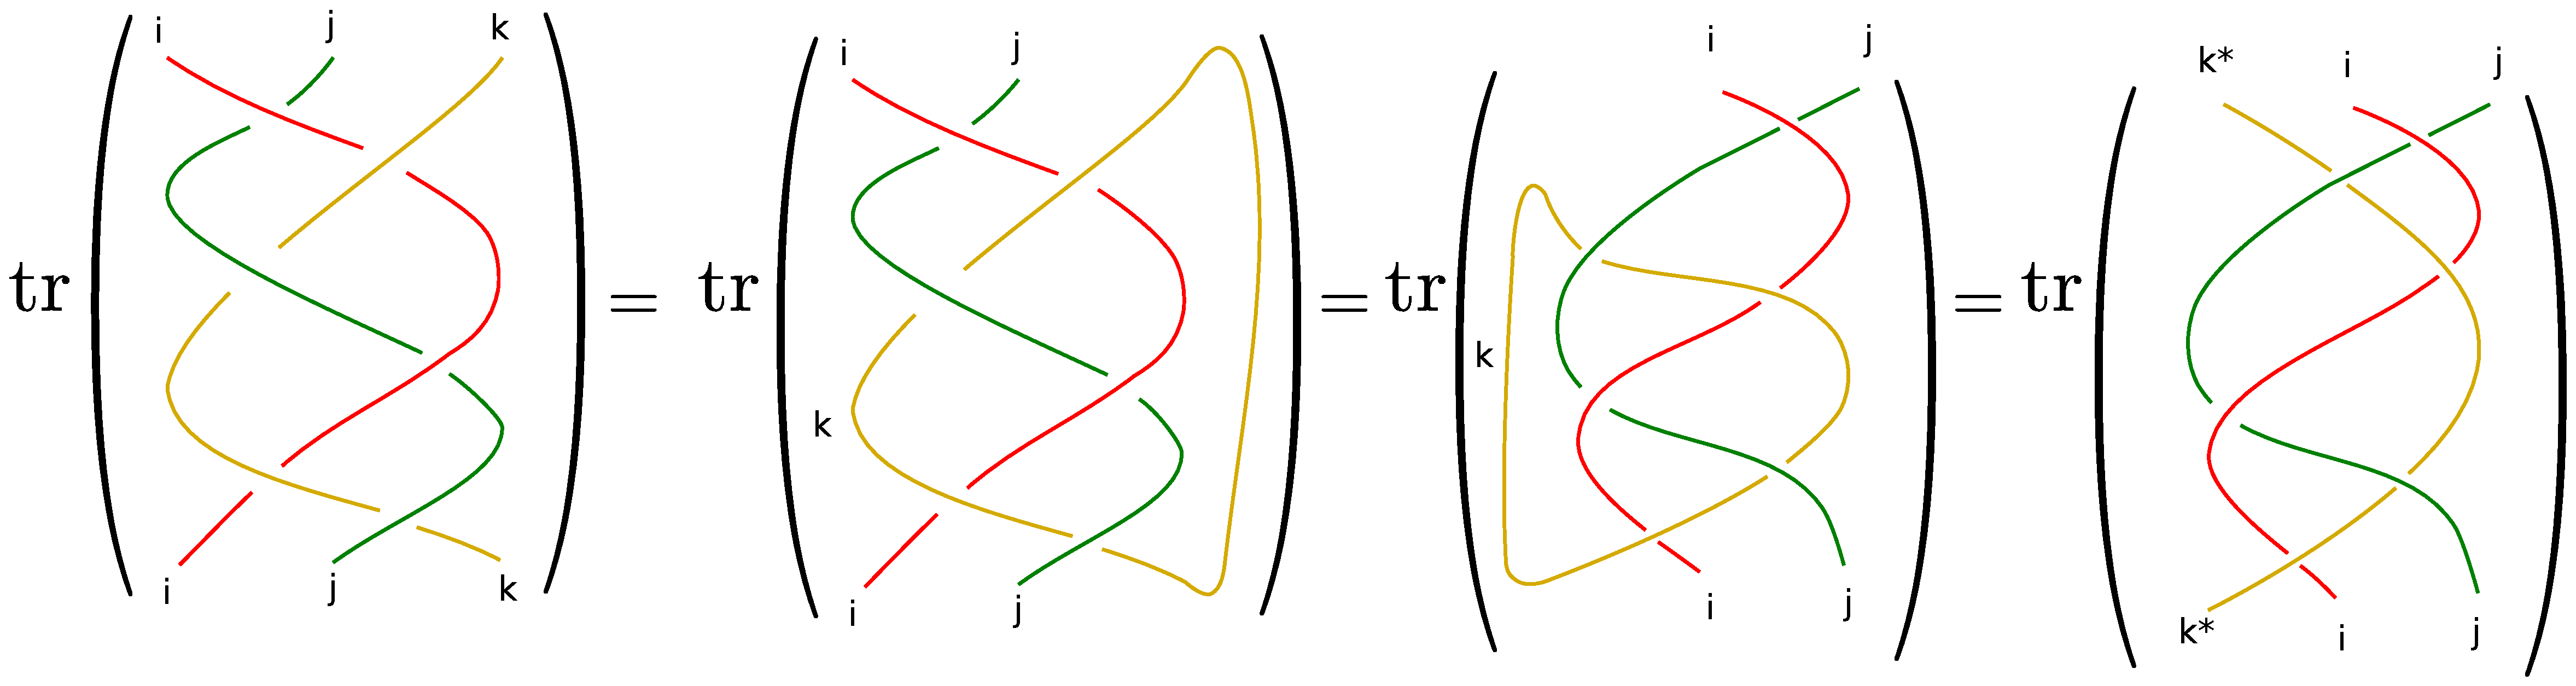
\includegraphics[width=0.9\textwidth]{final.eps}
\end{equation*}
Combining with \eqref{conjugated} we see that $B_{ijk}=B_{jik^*}$. Together with the cyclic permutation invariance, this yields that $B$ is invariant under any permutation of its indices combined with dualizing an even or odd number of its indices according to the parity of the permutation. If the borromean braid has finite order in the category in question (as is the case for group-theoretical modular categories, see \cite{MR2832261}), then $B_{ijk}$ is also the complex conjugate of the trace of the inverse Borromean braid. But the left hand side of \eqref{conjugated} is that trace, so $B_{ijk}=\overline{B_{kji}}$. So in this case $B$ is invariant under permutation and dualization of its indices, up to conjugation if the number of dualized indices has the opposite parity of the permutation.
\end{proof}
For larger rank categories, these symmetry properties could serve to speed up the computation of the borromean tensor, although, truth be told, we have so far only used them to debug our code.
\section{The B-tensor of a twisted double}\label{sec:borr-tens-twist}
\newcommand\Pe{P}

In this section we will derive an explicit formula for the borromean tensor in the Drinfeld center of a pointed fusion category, in terms of the group, the cohomological data, and the projective characters parametrizing the simple objects. It should be noted that in principle it is known how to obtain such formulas for the topological invariants defined by braided monoidal categories. Nevertheless it is a rather tedious undertaking to provide them in complete detail.


Consider three simple objects $ U, V, W \in  \mathcal{Z}(Vec^\omega_G)$, parametrized by couples $(g, \chi_1)$, $(h, \chi_2)$ and $(k, \chi_3)$. Take $u\in U_x, v\in V_y,  w\in W_z$, where $x\in \gb, y\in \hb, z\in \kb$.

Looking at the $G^3$-degree of tensors in $(U\ot V)\ot W$ (which is not affected by associativity isomorphisms), we see that for $u\in U_x$, $v\in V_y$, $w\in W_z$ we have
$\deg_{G^3}(R(\sigma_2\inv\sigma_1))(u\ot v\ot w)=\Pe(x,y,z)$ if we define $\Pe\colon G^3\to G^3$ by $\Pe(x,y,z)=(x\hit y,z,z\inv\hit x)$. Note $\Pe\inv(x,y,z)=(y\hit z,y\hit z\inv\hit x,y)$. Now in order that $((\sigma_2\inv\sigma_1)^3)_0(u\ot v\ot w)\neq 0$, we need to have $\Pe^3(x,y,z)=(x,y,z)$, or equivalently $\Pe^2(x,y,z)=\Pe\inv(x,y,z)$. Comparing
\begin{align*}
  \Pe^2(x,y,z)&=\Pe(x\hit y,z,z\inv\hit x)\\
            &=((x\hit y)\hit z,z\inv\hit x,(z\inv\hit x\inv)\hit x\hit y)\\
            &=((x\hit y)\hit z,z\inv\hit x,[z\inv,x\inv]\hit y)\\
  \Pe\inv(x,y,z)&=(y\hit z,y\hit z\inv\hit x,y)
\end{align*}
we see that:
\begin{align}
  ((\sigma_2\inv\sigma_1)^3)_0&|_{U_x\ot V_y\ot W_z}\neq 0\notag\\
                            & \Leftrightarrow
                              \begin{cases}(x\hit y)\hit z=y\hit z\\
                                z\inv\hit x=y\hit z\inv\hit x\\
                                [z\inv,x\inv]\hit y=y
                              \end{cases}\notag\\
                            &\Leftrightarrow\label{eq:condition0}
                              \begin{cases}[[y\inv,x],z]=1\\
                                [[z,y],x]=1\\
                                [[z\inv,x\inv],y]=1
                              \end{cases}
\end{align}

We evaluate the morphism $R((\sigma_2\inv\sigma_1)^3)$ in three steps.
\begin{align*}
  R(\sigma_2\inv\sigma_1)&((u\ot v)\ot w)\\
                         :&=\Phi(V\ot\sigma\inv)\Phi\inv(\sigma\ot W)((u\ot v)\ot w)\\
  &=\Phi(V\ot\sigma\inv)\Phi\inv((x\hit v\ot u)\ot w)\\
  &=\Phi(V\ot\sigma\inv)(\omega(x\hit y,x,z)(x\hit v\ot(u\ot w))\\
  &=\Phi(\omega(x\hit y,x,z)(x\hit v\ot (w\ot z\inv\bhit u)\\
                         &=\omega\inv(x\hit y,z,z\inv\hit x)\omega(x\hit y,x,z)(x\hit v\ot w)\ot z\inv\bhit u\\
                         &=\psi(x,z\inv\hit x,x\hit y,z)\Psi((u\ot v)\ot w)
 \end{align*}
 with
 \begin{align*}
   \psi(x,x',y,z)&=\omega\inv(y,z,x')\omega(y,x,z)\alpha_x\inv(z,z\inv)\\
              &=\omega\inv(y,z,x')\omega(y,x,z)\alpha_{x'}\inv(z\inv,z)\\
            \Psi(u\ot v\ot w)&=(|u|\hit v\ot w)\ot |w|\inv\hit u
\end{align*}
Further
\begin{multline*}
  R(\sigma_2\inv\sigma_1)((x\hit v\ot w)\ot z\inv\hit u)\\
  =\psi(x\hit y,(z\inv\hit x)\inv\hit(x\hit y),(x\hit y)\hit z,z\inv\hit x)\Psi((x\hit v\ot w)\ot z\inv\hit u)
  \\ 
  =\psi(x\hit y,y,y\hit z,z\inv\hit x)\Psi((x\hit v\ot w)\ot z\inv\hit u)\\
\end{multline*}
where
\begin{multline*} \Psi((x\hit v\ot w)\ot z\inv\hit u)\\
  =\alpha((z\inv\hit x)\inv, x)((x\hit y)\hit w\ot z\inv\hit u)\ot [z\inv,x\inv]\hit v\\
  \in W_{(x\hit y)\hit z}\ot U_{z\inv\hit x}\ot V_{[z\inv,x\inv]\hit y}=W_{y\hit z}\ot U_{z\inv\hit x}\ot V_y.
\end{multline*}
Further,
\begin{multline*}
  R(\sigma_2\inv\sigma_1)(((x\hit y)\hit w\ot z\inv\hit u)\ot[z\inv,x\inv]\hit v)\\
  =\psi(y\hit z,y\inv\hit(y\hit z),(y\hit z)\hit(z\inv\hit x),y)\Psi((x\hit y)\hit w\ot z\inv\hit u\ot[z\inv,x\inv]\hit v)\\
  =\psi(y\hit z,z,x,y)\Psi((x\hit y)\hit w\ot z\inv\hit z\ot[z\inv,x\inv]\hit v)\\
\end{multline*}
\begin{multline*}
\Psi((x\hit y)\hit w\ot z\inv\hit z\ot[z\inv,x\inv]\hit v) \\
  =\alpha_x(y\hit z, z\inv)\alpha_z(y, x\hit y)\psi(y\hit z,z,x,y)([y,z]\hit u\ot [z\inv,x\inv]\hit v\ot[y,x]\hit w.
\end{multline*}
Thus
\begin{multline*}
  R((\sigma_2\inv\sigma_1)^3((u\ot v)\ot w)\\
  =\Omega(x,y,z)[y,z]\hit u\ot[z\inv,x\inv]\hit v\ot [y,x]\hit w
\end{multline*}
with
\begin{multline}\label{omega}
\Omega(x,y,z)=\psi(x,z\inv\hit x,x\hit y,z)\psi(x\hit y,y,y\hit z,z\inv\hit x)\psi(y\hit z,z,x,y)\\
  =\omega(x\hit y,z,z\inv\hit x)\omega\inv(x\hit y,x,z)\alpha_x\inv(z,z\inv)\\
  \omega(y\hit z,z\inv\hit x,y)\omega\inv(y\hit z,x\hit y,z\inv\hit x)\alpha_y\inv(z\inv\hit x\inv,z\inv\hit x)\\
  \omega(x,y,z)\omega\inv(x,y\hit z,y)\alpha_z(y\inv,y)
\end{multline}

We conclude that
\begin{align*}
  B&_{(g,\chi_1),(h,\chi_2),(k,\chi_3)}\\&=\tr(R((\sigma_2\inv\sigma_1)^3))\\
  &=\tr(R((\sigma_2\inv\sigma_1)^3)_0)\\
  &=\sum_{\substack{x\in\ol g,y\in\ol h,z\in\ol k\\~(\cref{eq:condition0})}}\Omega(x,y,z)\chi_1^x([y,z])\chi_2^y([z\inv,x\inv])\chi_3^z([y,x]).
\end{align*}

Using \cref{trick}, we can reduce the three summations in the preceding formula to two.
\begin{align*}
  B&_{(g,\chi_1),(h,\chi_2),(k,\chi_3)}\\
   &=|\ol k|\sum_{\substack{x\in\ol g,y\in\ol h \\~(\cref{eq:condition1})}}\Omega(x,y,k)\chi_1^x([y,k])\chi_2^y([k\inv,x\inv])\chi_3([y,x])\\
   &=|\ol k|\sum_{\substack{x\in\ol g,y\in\ol h \\~(\cref{eq:condition1})}}
  \begin{aligned}[t]
    \Omega&(x,y,k)\alpha_{g} ([y, k], p)\alpha^{-1}_{g}(p, p^{-1} \hit [y, k])\\
    &\alpha_{h}([k^{-1}, x^{-1}],q) \alpha^{-1}_{h} (q, q^{-1} \hit [k^{-1},x^{-1}])\\
    &\chi_1^x([y,k])\chi_2^y([k\inv,x\inv])\chi_3([y,x]).
  \end{aligned}
\end{align*}
with
\begin{equation}\label{eq:condition1}
  \begin{aligned}[c]
    [[k, y], x] &= 1\\
    [[y^{-1}, x],k]&=1
  \end{aligned}
\end{equation}
Finally, we can express the characters $\chi_1^x$, $\chi_2^y$ in terms of $\chi_1,\chi_2$ using (\cref{chi}):
\begin{align}
  B&_{(g,\chi_1),(h,\chi_2),(k,\chi_3)}\notag\\
   &=|\ol k|\sum_{\substack{p\in G/C_G(g)\\q\in G/C_G(g)\\~(\cref{eq:condition3})}}
  \begin{aligned}[t]\Omega(p\hit g&,q\hit h,k)(p\hit\chi_1)([q\hit h,k])\\
    &(q\hit \chi_2)([k\inv,p\hit g\inv])\chi_3([q\hit h,p\hit g])  
  \end{aligned}\\
   &=\frac{|\ol g||\ol h||\ol k|}{|G|^2}\sum_{\substack{p\in G\\q\in G
  \\~(\cref{eq:condition3})}}\label{eq:1}
  \begin{aligned}[t]\Omega(p\hit g&,q\hit h,k)(p\hit\chi_1)([q\hit h,k])\\
    &(q\hit \chi_2)([k\inv,p\hit g\inv])\chi_3([q\hit h,p\hit g])  
  \end{aligned}
\end{align}
with
\begin{equation}
\label{eq:condition3}
\begin{aligned}[c]
 [[k, q\hit h], p\hit g] &= 1\\ 
 [[(q\hit h)^{-1}, p\hit x],k]&=1.
\end{aligned}
\end{equation}
Besides the $\omega$ and $\alpha$ terms already hiding in $\Omega$, the conjugated characters in the last formulae are hiding further $\alpha$ terms from (\cref{chi}):
\begin{align*}
  (p\hit \chi_{1})([q\hit h, k]) &=\begin{aligned}[t]\alpha_{g} ([q\hit h, k], p) \alpha^{-1}_{g}(p, p^{-1} \hit [q\hit h, k])\\\cdot\chi_1(p^{-1} \hit [q\hit h, k])&
  \end{aligned}
  \\
(q\hit \chi_{2})([k^{-1}, p\hit g^{-1}])&=\begin{aligned}[t] \alpha_{h}([k^{-1}, p\hit g^{-1}],q) \alpha^{-1}_{h} (q, q^{-1} \hit [k^{-1}, p\hit g^{-1}])&\\\cdot\chi_2(q^{-1}\hit[k^{-1}, p\hit g^{-1}])&
\end{aligned}
\end{align*}


We have implemented the general formula for the $B$-tensor above in GAP; the codes are in \cref{codes}. For explicit calculations by humans, the abundance of cocycle terms (six $\omega$ terms and three $\alpha$ terms gathered in $\Omega$ plus four $\alpha$ terms hiding in conjugated projective characters) and the tedious commutation conditions on group elements certainly make the formulas somewhat unwieldy. We will now describe particular circumstances where these problems do not occur and the formula simplifies drastically. The special cases will be very useful for the key example we will treat in the following section.

\begin{Prop} Suppose there is an abelian normal subgroup $A\triangleleft G$ such that  $\omega$ is inflated from the quotient $G/A$ , and $g,h\in A$. Then
  \begin{equation}
    \label{eq:simplified}
    B_{(g,\chi_1),(h,\chi_2),(k,\chi_3)}=\vert \overline k \vert \cdot \sum_{\substack{x\in \overline g\\y\in\overline h}}\chi_1(p\inv\hit[y,k])\chi_2(q\inv\hit[k\inv,x\inv]).
  \end{equation}
  where $p\hit g=x,q\hit h=y$ in the sum. Note also that $\chi_1,\chi_2$ are ordinary characters in this case.
\end{Prop}
\begin{proof}
  The conditions are tailored to ensure that $\Omega(x,y,z)=1$ in \ref{omega}, since all values of $\omega$ where one argument is conjugate to $g$ or $h$ are trivial. The same holds for the $\alpha$ terms used in (\cref{chi}), since commutators with one element from $A$ also lie in $A$. Also, $[[k,q\hit h],p\hit g]=1$ for all $q,p$ since $q\hit h\in A$, hence $[k,q\hit h]\in A$, and $p\hit g\in A$. Finally $[q\hit h\inv,p\hit g]=1$ since $q\hit h,p\hit g\in A$ which is abelian, and in particular $[[q\hit h\inv,p\hit g],k]=1$.
\end{proof}
\begin{Cor}\label{Cor:verysimplified}
  Assume the hypotheses of the preceding corollary, and in addition that there is a subgroup $Q\subset C_G(k)$ such that $g^Q=\overline g$ and $h^Q=\overline h$. This applies for example when $G=A\semdir Q$ is a semidirect product of abelian groups. Then
  \begin{equation}
    \label{eq:verysimplified}
    B_{(g,\chi_1),(h,\chi_2),(k,\chi_3)}=\frac{\vert \ol k \vert |A|}{|C_Q(g)||C_Q(h)|} \cdot\sum_{q\in Q}\chi_2(q\hit[h,k])\chi_1(q\inv\hit[k\inv,g\inv]).
  \end{equation}
\end{Cor}
\begin{proof}
  We have bijections $Q/C_Q(g)\ni p\mapsto p\hit g\in \ol g$ and $Q/C_Q(h)\ni q\mapsto q\hit h\in \ol h$, and therefore, abbreviating $N=|C_Q(g)||C_Q(h)|$,
  \begin{align*}
    B&_{(g,\chi_1),(h,\chi_2),(k,\chi_3)}\\&=\frac{\vert\ol k  \vert}N \cdot \sum_{p,q\in Q}\chi_1(p\inv\hit[q\hit h,k])\chi_2(q\inv\hit[k\inv,p\hit g\inv])\\
                                        &=\frac{\vert\ol k  \vert}N \cdot\sum_{p,q\in Q}\chi_1(p\inv q\hit[h,q\inv\hit k])\chi_2(q\inv p\hit[p\inv \hit k\inv,g\inv])\\
                                        &=\frac{\vert\ol k  \vert}N\cdot\sum_{p,q\in Q}\chi_1(p\inv q\hit[h,k])\chi_2(q\inv p\hit[k\inv,g\inv])
  \end{align*}
  which gives the desired result after reparametrization.
\end{proof}

\section{Twisted doubles of nonabelian groups of order $pq$}\label{sec:Example}
Let $p,q$ be odd primes with $p|q-1$. There is a unique nonabelian group of order $pq$, and there are exactly $p$ inequivalent twisted doubles of that group; see \cite{2017arXiv170802796M} and below. However, these $p$ inequivalent modular categories only afford three different sets of modular data. In this section we will show that the $T$-matrix and the borromean tensor do distinguish the $p$ modular categories. We first tested this for the case $p=5$ and $q=11$ using our GAP-implementation of~(\cref{eq:1}). That is, we computed the values of $T$-matrix, $S$-matrix, and $B$-tensor in this case, and verified that no bijection between the simples of two distinct categories maps all three data to each other. Closer inspection of the experimental data also helped us pick out the particular simples to use in our borromean tensor calculations below. Thus, although no computer help is necessary in the end to prove our results, machine calculations were instrumental in  our finding them. Note that the $S$-matrix turns out not to be necessary in our example in the end; the $T$-matrix and $B$-tensor suffice.



The nonabelian group of order $pq$ where $p$ and $q$ are odd primes such that $p | q-1$ has the following presentation:
$$
\ZZ/q\ZZ \semdir \ZZ/p\ZZ \cong \langle a,b | a^q=b^p=1 ,\ bab^{-1}=a^n \rangle
$$
The integer $n \in \ZZ/q\ZZ$ must be chosen such that $n \not\equiv 1 \mod q$ and $n^p \equiv 1 \mod q$, but the group does not depend on that choice.
We note
\begin{align}\label{eq:pqformulas}
  b^k a^l b^{-k} &= a^{n^k l} &
  [a^l,b^k]&=a^{l(1-n^k)}&
  [b^k,a^l]&=a^{l(n^k-1)}
\end{align}


The canonical surjection $\ZZ/q\ZZ \semdir \ZZ/p\ZZ\to \langle b\rangle\cong\ZZ/p\ZZ$ induces an isomorphism between the cohomology groups $H^3(\langle b\rangle ,\CCu)\to H^3(\ZZ/q\ZZ \semdir \ZZ/p\ZZ,\CCu)$, where $H^3(\langle b\rangle ,\CCu)\cong \ZZ/p\ZZ$ is generated by the following cocycle $\omega$:
$$
\omega(b^i,b^j,b^k):=\exp\left( \frac{2i\pi}{p^2}([i]([j]+[k]-[j+k])\right)
$$
where $[i]\in\{0,\dots,p-1\}$ is such that $[i]\equiv i(\mod p)$.

The following is a complete list of representatives for the isomorphism classes of simples of $\CTR(\Vect_G^{\omega^u})$:
\begin{enumerate}
\item
$(1,\chi)$ where $\chi$ is an irreducible character of $G$,
\item
$(a^l,\chi_q^s)$ where $l\in (\ZZ/q\ZZ)^\times/\langle n\rangle$, $s\in\ZZ/q\ZZ$,
and $\chi_q$ is the generator of $\widehat{\langle a \rangle}\cong \ZZ/q\ZZ$ given by
$$
\chi_q(a)=\exp\left(\frac{2i\pi}{q}\right),
$$ 
\item
$(b^k,\widetilde{\chi_p^r})$ where $k\in\ZZ/p\ZZ^\times$, $r\in \ZZ/p\ZZ$, and $\widetilde{\chi_p^r}$ is the $\alpha_{b^k}^u$-projective character of $C_G(b^k)=\widehat{\langle b \rangle}$ associated to $\chi_p^r$, $\chi_p$ being the generator of $\widehat{\langle b \rangle}\cong \ZZ/p\ZZ$ given by
$$
\chi_p(b)=\exp\left(\frac{2i\pi}{p}\right).
$$ 
That is $\widetilde{\chi_p^r}=\chi_p^r \mu_{b^k}^u$ where $\alpha_{b^k}^u=d \mu_{b^k}^u$. In the sequel, we will write the simple as $(b^k,\chi_p^r)$ instead of $(b^k,\widetilde{\chi_p^r})$.
\end{enumerate}
\begin{Lem}\label{TLem}
The $T$-matrix of $\CTR(\Vect_G^{\omega^u})$ is given by the following:
\begin{enumerate}
\item
$\Theta(1,\chi)=1$
\item
$\Theta(a^l,\chi_q^s)=\exp\left(\frac{2i\pi}{q}sl\right)$
\item
$\Theta(b^k,\chi_p^r)=\exp\left(\frac{2i\pi}{p^2}(pkr+k^2u)\right)$, and in particular
\item $\Theta(b^k,\chi_p^r)^p=\zeta_p^{k^2u}$ for $\zeta_p=\exp(\frac{2i\pi}{p})$.
\end{enumerate}
\end{Lem}
\begin{proof}
For simples in $\CTR(\Vect_G^{\omega^u})$ of the first type, it is obvious that the corresponding twist $\Theta(1,\chi)=\frac{\chi(1)}{\chi(1)}=1$. For simples of the second type $(a^l,\chi_q^s)$, one has $\alpha_{a^l}^u=1$, and then the irreducible projective characters of the centralizer $\langle a \rangle \cong \ZZ/q\ZZ$ of $a^l$ are the usual irreducible characters. The twist is therefore given by 
$$
\Theta(a^l,\chi_q^r)=\frac{\chi_q^s(a^l)}{\chi_q^s(1)}=\exp\left(\frac{2i\pi}{q}sl\right)
$$
Finally, for simples of the last type $(b^k,\chi_p^r)$, one has $\alpha_{b^k}^u=d \mu_{b^k}^u$ where
$$
\mu_{b^k}^u(x)=\exp\left(\frac{2i\pi u}{p^2}k[\Pi(x)]\right)
$$
and $\alpha_{b^k}^u$-projective characters of the centralizer $\langle b \rangle \cong \ZZ/q\ZZ$ of $b^k$ are usual irreducible characters twisted by $\mu_{b^k}^u$. Therefore:
$$
\Theta(b^k,\chi_p^r)=\frac{\chi_q^r(b^k)\mu_{b^k}^u(b^k)}{\chi_q^r(1)\mu_{b^k}^u(1)}=\exp\left(\frac{2i\pi}{p^2}(pkr+k^2u)\right)
$$
\end{proof}

\begin{Lem}\label{BProp} The $B$-tensor of the category $\CTR(\Vect_{\ZZ/q\ZZ \semdir \ZZ/p\ZZ}^{\omega^u})$ with $p$ and $q$ odd primes such that $q|p-1$ and $u\in\{0,\dots p-1\}$ satisfies
\begin{equation}
B_{(a^l,\chi_q^s),(a^l, \chi_q^s),(b^{k}, \chi_p^r)}=p q \sum_{m=0}^{p-1} e^{\left(\frac{2i\pi sl}{q} (n^{-t}-n^t)(n^m-n^{-m})\right)};\quad 2t\equiv k(p) 
\end{equation}
\end{Lem}

\begin{proof}
We apply \cref{Cor:verysimplified} with $Q=\langle b\rangle$ and $A=\langle a\rangle$.
By \cref{eq:verysimplified} and \cref{eq:pqformulas} we have
\begin{align*}
  B_{(a^l,\chi_q^s),(a^l, \chi_q^s),(b^k, \chi_p^r)} &=pq\sum_{m=0}^{p-1}\chi_q^s(b^m \hit[a^l,b^k])\chi_q^s(b^{-m} \hit[b^{-k},a^{-l}] )\\
  &=p q \sum_{m=0}^{p-1} \chi_q^s(a^{l \cdot n^m (1-n^k)})\chi_q^s(a^{-l \cdot n^{-m} (n^{-k}-1)})\\
&= p q \sum_{m=0}^{p-1} e^{\left(\frac{2i\pi sl}{q} (n^{m}(1-n^k)+n^{-m}(1-n^{-k})\right)}.
\end{align*}
For $2t\equiv k(p)$ we get
\begin{align*}
  n^{m}(1-n^k)+n^{-m}(1-n^{-k})&\equiv n^m(1-n^{2t})+n^{-m}(1-n^{-2t})\\&=(n^{m+t}-n^{-(m+t)})(n^{-t}-n^t)
\end{align*}
so reparametrization gives the desired expression.
\end{proof}



In \cite{2017arXiv170802796M} it was shown that the $p$ non-equivalent modular tensor categories  $\CTR(\Vect_{\ZZ/q\ZZ \semdir \ZZ/p\ZZ}^{\omega^u})$ for $u=0,..,p-1$, are not distinguished by their modular data. In fact there are only three different modular data between these categories. By contrast:
\begin{Thm}\label{mainthm}
The $T$-matrix and $B$-tensor form a complete set of invariants for the $p$ non-equivalent modular categories $\CTR(\Vect_{\ZZ/q\ZZ \semdir \ZZ/p\ZZ}^{\omega^u})$ where $p$ and $q$ are odd primes such that $p|q-1$. More precisely, if there is a map $\kappa$ from the simple objects of $\CTR(\Vect_{\ZZ/q\ZZ \semdir \ZZ/p\ZZ}^{\omega^u})$ to the simple objects of $\CTR(\Vect_{\ZZ/q\ZZ \semdir \ZZ/p\ZZ}^{\omega^{u'}})$ satisfying $T_{\kappa(V)}=T_{V}$ and $B_{\kappa(U),\kappa(V),\kappa(W)}=B_{UVW}$ for all simples $U,V,W$ of the former, then $u=u'$.
\end{Thm}
\begin{proof}
  Let $\kappa$ be such a map. We will use the notations $(g,\chi)_u$ and $(g,\chi)_{u'}$ to denote simple objects of the two categories under consideration. The category corresponding to the trivial cocycle is easily distinguished from the others by the $T$-matrix alone, so we can assume $u,u'\neq 0$. Let $ls\not\equiv 0(\mod q)$. Then it is obvious from \cref{TLem} that $\kappa((a^l,\chi_q^s)_u)=(a^{l'},\chi_q^{s'})_{u'}$ with $sl \equiv s'l' \mod q$. Also, part (4) of \ref{TLem} implies that $\kappa((b^k,\chi_p^r)_u)=(b^{k'},\chi_p^{r'})_{u'}$ for some $k'$ and $r'$ with $k'^2u'\equiv k^2u(\mod p)$.

Also
\begin{align*}
B_{(a^l,\chi_q^s)_u,(a^l, \chi_q^s)_u,(b^k, \chi_p^r)_u} &= B_{\kappa((a^l,\chi_q^s)_u),\kappa((a^l, \chi_q^s)_u),\kappa((b^k, \chi_p^r))}\\
&= B_{(a^{l'},\chi_q^{s'})_{u'},(a^{l'},\chi_q^{s'})_{u'},(b^{k'}, \chi_p^{r'})_{u'}}
\end{align*}
So, with \cref{BProp} and $2t\equiv k(\mod p), 2t'\equiv k'(\mod p)$, we get
\begin{equation}\label{sumroots}
\sum_{m=0}^{p-1} \left(e^{\frac{2i\pi sl} {q} }\right)^{(n^t-n^{-t})(n^{m}-n^{-m})} = \sum_{m=0}^{p-1} \left(e^{\frac{2i\pi s'l'} {q} }\right)^{(n^{t'}-n^{-t'})(n^{m}-n^{-m})}.
\end{equation}
Since this is a $\mathbb Q$-linear relation between fewer than $q$ powers of the same primitive $q$-th root of unity $e^{\frac{2i\pi sl} {q} }=e^{\frac{2i\pi s'l'} {q}}$, we conclude that the set 
\begin{equation*}
  M_t:=\{(n^t-n^{-t})(n^{m}-n^{-m})|m=0,\dots,p-1\}\subset\ZZ/q\ZZ
\end{equation*}
is equal to the analogous set $M_{t'}$. We note that the $p$ elements $n^m-n^{-m}$ are distinct: Indeed, assume $n^m-n^{-m}=n^j-n^{-j}$ for $0\leq m,j\leq p-1$. Then
  \begin{equation*}
    0=n^m-n^j+n^{-j}-n^{-m}=(n^{-j-m}+1)(n^m-n^j).
  \end{equation*}
 Now $n^{-j-m}+1\neq 0$ since $n$ has odd order, and so $n^m=n^j$ which implies $m=j$. In particular
\begin{align*}
  \sum_{x\in M_t}x^2&=\sum_{m=0}^{p-1}(n^{t}-n^{-t})^2(n^{2m}+n^{-2m}-2)\\
                  &=(n^{t}-n^{-t})^2\left(\sum_{m=0}^{p-1}n^{2m}+\sum_{m=0}^{p-1}n^{-2m}-2p\right)\\
  &=-2p(n^{t}-n^{-t})^2,
\end{align*}
since $n^2$ and $n^{-2}$ are primitive $p$-th roots of unity in $\ZZ/q\ZZ$
and so the sum over all their powers gives zero. By the same reasoning
\begin{equation*}
  \sum_{x\in M_t}x^2=\sum_{x\in M_{t'}}x^2=-2p(n^{t'}-n^{-t'})^2
\end{equation*}
Thus $(n^t-n^{-t})^2=(n^{t'}-n^{-t'})^2$, which implies $n^t-n^{-t}=n^{t'}-n^{-t'}$ or $n^t-n^{-t}=n^{-t'}-n^{t'}$. As we have seen, this implies $t\equiv t'$ or $t\equiv -t'$ in $\ZZ/p\ZZ$. Therefore $k^2=k'^2$ and we can conclude that $u=u'$.
\end{proof}

\begin{Rem}\rm
  There is an action of the absolute Galois group of abelian extensions  of the rationals $\Gamma:=\Gal(\Q^\ab/\Q)$ on the set of simples of any integral modular category; see \cite[Appendix]{EtiNikOst:FC}. In the case of $\CTR(\Vect_G^\omega)$ it satisfies $S_{\gamma(i),\gamma(j)}=\gamma^2(B_{i,j})$ for any $\gamma\in\Gamma$, and also $T_{\gamma(i),\gamma(i)}=\gamma^2(T_{ii})$ as shown in  \cite{MR3435813}. If we analyze the proof in \cite{2017arXiv170802796M} that the twisted doubles of nonabelian groups of order $pq$ share only three different sets of modular data, we can conclude from our result that the analogous property $B_{\gamma(i),\gamma(j),\gamma(k)}=\gamma^2(B_{ijk})$ is not satisfied. 
\end{Rem}

\section{Square-free groups and their twisted doubles} % (fold)
\label{sub:twisted_doubles_of_square-free groups}
% subsection twisted_doubles_of_square (end)
Groups of square-free order (or simply square-free groups) have been classified over a century ago by H\"older\cite{Hoelder1895}. We will briefly describe their structure and classification, and also briefly look at the structure of their twisted doubles.

For a square-free group $G$ order $|G| = \prod_{i=1}^z p_i$, where $p_i$ are distinct primes such that $p_i <p_{i+1}$, H\"older gave a formula for the number of isomorphic groups of a given order. We however use an algorithmic approach to calculate the number of square-free groups of a given order due to Alonso \cite{MR506898}.\\ 
Any square-free group can be presented in the following way,  
\begin{equation}\label{presentation}
	G= <a_i (1\leq i\leq z)| a_i^{p_i} =1, a_j\hit a_i = a_i^{n_{ij}} (1\leq j<i\leq z)>
\end{equation}
where $n_{ij}$ is referred to as the action of $a_j$ on $a_i$ and is a solution to the equation \begin{equation}\label{act-condition}
	n_{ij}^{p_j}\equiv 1 \mod p_i.
\end{equation} For each pair $(p_i, p_j)$ such that $p_j|p_i-1$ and $n_{ij}$ is non-trivial, the set of solutions of the equation (\ref{act-condition}) forms a cyclic group of order $p_j$, $\ZZ_{p_j}^\times$ for which we will sometimes pick a generator $N_{ij}$ for this group.
If $(p_i, p_j) $and $(p_j, p_t)$ (with $t<j<i$) are two such pairs, the element $a_j\hit a_i = a_i^{n_{ij}}$ can be conjugated by $a_t$ \begin{align*}
a_t\hit(a_j\hit a_i) &= a_t\hit a_i^{n_{ij}}\\
	(a_t\hit a_j)\hit(a_t\hit a_i) &= (a_t\hit a_i)^{n_{ij}}\\
	a_j^{n_{jt}}\hit a_i^{n_{it}} &= a_i^{n_{ij}n_{it}}
\end{align*}
and since $a_j^x\hit a_i^y = a_i^{yn_{ij}^x}$, we get\begin{equation*}
	a_i^{n_{ij}n_{it}} = a_i^{n_{it}n_{ij}^{n_{jt}}} \end{equation*} 
and thus
\begin{equation*}
	n_{ij}^{n_{jt} -1} \equiv 1 \mod p_i
\end{equation*}
so we have \begin{equation}\label{non-cont}
	\text{for } t<j<i, \quad n_{ij} \equiv 1 \mod p_i \quad \text{or}\quad n_{jt} \equiv 1 \mod p_j.
\end{equation} From now on, we will abuse language and say that a prime factor $p_j$ ``acts'' on a prime factor $p_i$, or equivalently that $p_i$ is ``acted upon" by $p_j$, when we mean that the subgroup $C_{p_j}$ acts non-trivially on the subgroup $C_{p_i}$. The condition (\ref{non-cont}) means that every prime factor can either act or be acted upon, or neither, but not both. A choice such as $n_{ij} =N_{ij}^w$ where  $w>1$, can be turned into $n_{ij} =N_{ij}$ by picking a different generator $a_j'= a_j^w$. In fact, we can assume that \begin{equation}\label{possible}
	\text{ if $1 = n_{i1} =n_{i2} =\dots =n_{i, j-1}$  then $n_{ij}= 1$ or $N_{ij}$.}
\end{equation} 
The existence of groups with presentation (\ref{presentation}) and conditions (\ref{act-condition}), (\ref{non-cont}) and (\ref{possible}) is shown in the text \cite[Section 9.2.2]{MR896269}, it is simply the group $\ZZ_q\semidir_n \ZZ_p$, where $q$ is product of the factors which are acted upon, and $p$ is the product of the factors which act, whereas $n$ denotes the action $\ZZ_p$ on $\ZZ_q$.  \begin{Prop}\label{uniqueness}
Two presentations of type (\ref{presentation})  with conditions (\ref{act-condition}), (\ref{non-cont}) and (\ref{possible}) that differ in at least one of the exponents $n_{ij}$ give non-isomorphic groups.
\end{Prop}
This proof is taken from \cite{MR506898}. We need a small lemma before we prove this.
\begin{Lem}[Hall]\label{hall}
If $A$ is a finite solvable group of order $uv$ and $(u,v) = 1$, then there is at least one subgroup of order $u$ and any two such subgroups are conjugate.
\end{Lem}
\begin{proof}[Proof of Proposition \ref{uniqueness}]
Consider two groups $G$ and $G'$ of type (\ref{presentation}) with generators $a_i$ and $a_i', (1\leq i \leq z)$, obeying conditions (\ref{act-condition}), (\ref{non-cont}) and (\ref{possible}). 
In order to use an inductive argument, let the proposition be true for groups with $z-1$ generators. Let $n_{ij}\neq n'_{ij}$ for some $j< i$. 
If $i< z$ then $<a_1,a_2,\dots, a_{z-1}> \not\cong <a'_1,a'_2,\dots, a'_{z-1}>$, and so $G\not\cong G'$ by Lemma \ref{hall}. Now if $n_{ij} = n'_{ij}$ for $1\leq i<j<z$, and if $n_{z1}\neq n'_{z1}$ then one of them is 1 and the other is $N_{z,1}$ by (\ref{possible}). so $<a_1, a_z> \not \cong <a'_1, a'_z>$, and by Lemma \ref{hall} $G\not\cong G'$. So assume that $n_{z1} = n'_{z1}$ and let $i$ be the smallest index such that $n_{z i}\neq n'_{zi}$ and assume $n'_{z i}\neq 1$, by (\ref{non-cont}) $n_{ij} = n'_{ij}=1$ for all $j<i$. If $n_{z j} = n'_{zj} = 1$ for all $j<i$ then $n_{zi} = 1$ and $n'_{zi} = N_{zi}$. Hence $<a_1, a_i, a_n>$ is abelian while $<a'_1, a'_i, a'_n>$ is not, so $G\not\cong G'$ by Lemma \ref{hall}. Else, let $j$ be the smallest index such that $n_{zj} = n'_{zj} \neq 1$. Then by (\ref{possible}), $n_{zj} = n'_{zj} = N_{zj}$, so $<a'_j, a'_i, a'_z>$ has actions $N_{zj}, N_{zi}^w$ for $w \mod p_i$ whereas $<a_j, a_i, a_z>$ either is also of this type with actions $N_{zj}, N_{zi}^{w\prime}$ where $w'\not\equiv w \mod p_i$ or has $<a_i, a_z>$ abelian. Thus $G\not\cong G'$ by Lemma \ref{hall}. 
\end{proof}
\begin{Rem}\label{chinese}\rm
For an element $a\in Q$, the actions of any two non-trivially acting elements of $P$ generate cyclic groups of coprime order, and so by the Chinese remainder theorem we may denote the action by a single number $n_a$ whose order mod $q_a$ is the product of all $p_j\in P$ such that $b_j$ acting non-trivially on $a$. Again by the Chinese remainder theorem, there is a unique $n$ mod $q$ such that for each $a \in Q$, $n\equiv n_a \mod q_a$ where $q_a$ denotes the order of $a$. We call this $n$ the `action' associated with $G$ for obvious reasons, and along with $p$ and $q$ it determines the group (up to isomorphism).
\end{Rem}
For brevity, we may sometimes denote $G=\ZZ_q\semidir_n\ZZ_p$ as \begin{equation*}
	G = G_{p,q,n}.
\end{equation*}\\
Let $G$ be a finite group of odd square-free order $pq$. Let $P$ denotes a set of generators for cyclic subgroups corresponding to the prime factors of $p$, and $Q$ a set of generators for cyclic subgroups corresponding to the prime factors of $q$. 
Given $p,q$ such that $pq$ is odd square-free, it is possible to count the number of non-isomorphic groups of order $pq$. We calculate this number explicitly for two cases.\\
Suppose $p, q$ are primes, $p<q$. Picking generators for the two cyclic subgroups $<a>$ of order $q$, and $<b>$ of order $p$ such that $b\hit a=a^n$, since $a = b^p\hit a = a^{n^p}$, we must have\begin{equation*}
	n^p\equiv 1 \mod q.
\end{equation*} If $p|q-1$, the solutions to this equation mod $q$ form a cyclic subgroup of order $p$. Thus we have $p$ different choices of the action $b\hit a$, the trivial one corresponding to the abelian group of order $pq$, and the remaining $p-1$ non-trivial actions give the same group up to isomorphism. So there are two non-isomorphic groups of order $pq$ if $p|q-1$, else there is only one.

Now suppose $G$ has order $pqr$, where $p, q, r$ are prime, $p<q<r$. If we declare a condition like $p_j|p_i-1$ below, then we will want to know how many new groups emerge, and so we will consider a non-trivial action of the generator $a_j$ on $a_i$, because otherwise we end up with a known case. For example in the previous case, the abelian group of order $pq$ was known without imposing $p|q-1$.\\
\begin{enumerate}
	\item If $p\nmid q-1, p\nmid r-1$, and $q\nmid r-1$ there is only one possibility, the abelian group of order $pqr$. 
	\item If $p|q-1, p\nmid r-1, q\nmid r-1$, ( or if $p\nmid q-1, p| r-1, q\nmid r-1$) then the only new possibility is the direct product of the cyclic group of order $r$ (of order $q$) with the non-abelian group of order $pq$ (of order $pr$). 
	\item If $p|q-1,p|r-1, q\nmid r-1$, then using criterion (\ref{possible}) we find that there is only one non-trivial (upto isomorphism) choice for the action on the factor $C_r$, $n_{rp} = N_{rp}$ and subsequently, $p-1$ distinct choices of the action corresponding to non-trivial elements of $<N_{qp}>$. Hence there are $p-1$ new groups.	
\item If $p|r-1, q|r-1, p\nmid q-1$ then for both actions, there is only one non-trivial choice, so there is only one new group.
\item If $p|q-1, p|r-1$ and $q|r-1$, then either $n_{rq}$ or $n_{qp}$ is trivial, so our analysis breaks up into two cases. If $n_{rq}$ is trivial, then there are no new groups apart from those already present in the case $p|q-1, p|r-1, q\nmid r-1$, and if $n_{qp}$ is trivial then there are no new groups apart from those already present the case $p|r-1, q|r-1, p\nmid q-1$.\\
\end{enumerate}
Such an analysis could be done for a group of any square free order, simply by studying the possible actions. In the appendix, we have provided a GAP function which takes an input a square-free number $x$, and returns the number of non-isomorphic groups of order $x$, using an algorithm described in \cite{MR506898}. 

 For groups of a given square free order 
\begin{equation}\label{order}
	p_1p_2\dots p_kq_1q_2\dots q_l,\end{equation} 
  where the $p_j$'s are the acting factors, and the $q_i$'s are either acted upon or form a central subgroup, writing
 \begin{equation*}
  	p_1p_2\dots p_k;q_1q_2\dots q_l,
  \end{equation*} determines a class of square-free groups, all of which have a maximal abelian normal subgroup of order $q_1q_2\dots q_l$. H\"older refers to this class as a \textit{Gattung}, German for `genus'. 	 
  Now suppose a group $G$ belongs to the \textit{Gattung} represented by 
  \begin{equation*}
  	p_1p_2;q_1q_2
  \end{equation*}
and suppose that in $G$, $p_1$ acts non-trivially on $q_1$ while $p_2$ acts non-trivially on both $q_1$ and $q_2$. This may be denoted in the following way,
\begin{equation}\label{arten}
	\overbracket{p_1{\underbracket{\underbracket{p_2;q_1}q_2}}} 
\end{equation}
where a specific bracket denotes action of the prime factor from which it starts, on  the prime factor at which it ends, read left to right. Note that every prime factor $p_i$ must have at least one bracket starting from it, otherwise it is possible to consider it as a constituent of the normal subgroup, thus contradicting the fact that the largest abelian normal subgroup has order $q_1\dots q_l$. The group $G$ is surely not determined by the expression (\ref{arten}) as there may be several choices of the actions indicated. The expression thus represents a class of groups, which H\"older calls an \textit{Art} (plural \textit{Arten}), German for `species'. Every \textit{Gattung} consists of several \textit{Arten}, and every \textit{Art} consists of groups with the same acting and acted upon prime factors but different actions. In fact, we will see that two groups with equivalent twisted doubles must lie in the same \textit{Art}.

We are interested in studying Drinfeld centers of pointed fusion categories $\Vect^\omega_G$, denoted $\CTR(\Vect^{\omega}_{G})$, where $G$ is a square-free group. We will henceforth not distinguish between a simple object in $\CTR(\Vect^{\omega}_{G})$ and the couple $(g, \chi)$ representing its isomorphism class.
Recall that $Q$ is a set of generators for the maximal abelian normal subgroup $N$ of $G$, and $P$ a set of generators for the quotient group $G/N$. Apart from the trivial element, every element of $G$ is conjugate to an element of one of the following 3 types.\begin{enumerate}
\item $\prod_{i=1}^m a_i^{g_i}$ for distinct $a_i\in Q$ and each $g_i \in \ZZ_{q_i}^\times/<n_{a_i}> $ where $q_i$ is the order of the corresponding $a_i$ and $<n_{a_i}>$ is the subgroup generated by the non-trivial action of $\ZZ_p$ on $a_i$.
\item $ \prod_{j=1}^n b_j^{h_j} $ for distinct $b_j\in P$ and $h_j \in \ZZ_{p_j}^\times$ where $p_j$ is the order of $b_j$. 
\item $ \prod_{i=1}^m a_i^{g_i} \prod_{j=1}^n b_j^{h_j} $ such that every generator commute with every other. \end{enumerate}
Let $b_j\hit a_i = a_i^{n_{ij}}$. All the $b_j$'s commute and conjugation of $b_j^{h_j}$ by any $a_i$ does not change its power but only adds an $a_i$ factor (see \ref{a-action}), so no two elements of type (2) are conjugate. Products of non-commuting generators are accounted for as follows. For $a_i, b_j$ such that $[a_i, b_j]\neq1$, we have \begin{equation}
	a_i^{g_i}\hit b_j^{h_j} = a_i^{g_i(1-n_{ij}^{h_j})}b_j^{h_j}.\label{a-action}
\end{equation} The term $(1-n_{ij}^{h_j})$ is invertible, since $n_{ij}$ is a non-trivial action (as $[a_i, b_j]\neq 1$), and $h_j$, the power of $b_j$, is non-zero. Write $g_i'= g_i(1-n_{ij}^{h_j}) \in \ZZ_{q_i}^\times$ for $h_j\not\equiv 0 \mod p_j$, then $a_i^{g_i'}b^{h_j} = a^{g_i}\hit b^{h_j}$. Thus we see that every element $a_i^{g_i'} b_j^{h_j}$ is conjugate to $b_j^{h_j}$. More informally, for an element of the type $ a_1^{g_1}...a_m^{g_m}b_1^{h_1}...b_n^{h_n} $ such that some of the generators do not commute, we can simply omit the non-commuting $a_i$'s to arrive at a representative of type (2) or (3).
\begin{Rem}\label{char}\rm For a conjugacy class representative $r= \prod_{i=1}^m a_i^{g_i} \prod_{j=1}^n b_j^{h_j}$ of type (1), (2) or (3), the abelian subgroup  $H\subseteq C_G(r)$ generated by $\{a_i, b_j\}$ is a direct factor in $C_G(r)$.
\end{Rem} 
\begin{proof}
Suppose that  an  element of $C_G(r)$, $x=\prod_{i=1}^{t}c_i\prod_{j=1}^{s}d_j$ for distinct $c_i\in Q, d_j\in P$, does not lie in $H$.  By the Chinese remainder theorem,  for every $a_i$ there is a power $\pi_i$ of $r$ such that $r^{\pi_i} = a_i$ and also a power $\pi_j$ such that $r^{\pi_j} = b_j$, hence every $a_i, b_j\in H$ commutes with $x$. Similarly, for every $c_i$, there is a power $\pi'_i$ such that $x^{\pi'_i}= c_i$ and a power $\pi'_j$ such that $x^{\pi'_j} = d_j $,  hence every $c_i, d_j$ commutes with $r$. Let $K$ be the subgroup generated by those elements of $C_G(r) \cap(P\cup Q)$ that are not in $H$. Clearly $K$ is also a normal subgroup, and $H\cap K =\{1\}$ because the two subgroups have no other elements in common.  We conclude that $C_G(r)= K\times H$.
\end{proof}
By the multiplicativity of characters over direct products of groups, for an irreducible character $\chi_1$ of $C_G(r)$, \begin{equation*}
	\chi_1|_{H} = \chi_1(1)\varphi^v
\end{equation*} where $\varphi$ is a generator of $\hat{H}$, the group of characters on $H$, and $v$ is an integer mod $|H|$.


We now give formulae for certain $T$-matrix entries which will be useful later. For an element $a\in Q$ of order $\qb$, pick a generator $\varphi$ for the cyclic group of characters of $H=<a>$, the cyclic group generated by $a$, such that for a character $\chi_1$ of $C_G(a^g)$, $\chi_1|_{<a>} = \chi_1(1)\varphi^v$, for  some integral power $v$ defined mod $\qb$. Then,
 \begin{equation}\label{a}
	  \Theta(a^{g}, \chi_1) = \frac{\chi_1(a^{g})}{\chi_1(1)}
	= \frac{\chi_1(1)\varphi^v(a^{g})}{\chi_1(1)} 
	= \exp(\frac{2\pi iv g}{\qb}).
	\end{equation}
 Similarly, for an element $b\in P$ of order $\pb$, pick a generator $\psi$ for the cyclic group of characters of $H'=<b>$, the cyclic group generated by $b$, such that for a character $\chi_2$ of $C_G(b^h)$, $\chi_2|_{<b>} = \psi^w$, for some exponent $w$ defined mod $\pb$. Then we get
 \begin{equation*}
	 \Theta(b^{h}, \chi_2) = \tilde{\chi}_2(b^{h})\mu^u_{b^h}(b^h),
	 \end{equation*}
where $\mu^u_{b^h}$ is a 1-cochain, such that the multiplier of the projective character $\chi_2$, $\alpha_{b^k}^u = d\mu^u_{b^h}$. When the multiplier is a coboundary, the projective character is a scalar multiple of $\tilde{\chi}_2$, an ordinary character.  The quantity $\mu^u_{b^h}$ is defined as \begin{equation*}
	\mu_{b^h}^u (b^r) = \exp(\frac{2\pi iu}{\pb^2}[h][r]),
\end{equation*}
where $[-]$ denotes that the number is taken mod $\pb$. So finally,
\begin{equation*}
	 \Theta(b^{h}, \chi_2)	 = \frac{\chi_2(1)\varphi^w (b^{h})\mu^u_{b^h}(b^h)}{\chi_2(1)} 
	 =\exp (\frac{2\pi iwh}{\pb} + \frac{2\pi i}{\pb^2}[h]^2u).
\end{equation*}



\section{The S-matrix for twisted doubles of square-free groups} \label{squarefreeS}
In this section, we state and prove a theorem that gives necessary and sufficient conditions for when certain diagonal S-matrix entries of two twisted doubles of square-free groups can be equal. For $a\in Q$ of order $q_a$, let $P_a = \{b_1,\dots,b_z\}$  be the set of generators which act non-trivially on $a$, with actions $n_1,\dots, n_z$ and orders $\pb_1,..., \pb_z$, with $p_a$ the product of these orders. In the following theorem, we abuse notation and denote the generator of the cyclic subgroup of order $q_a$ in both $G$ and $G'$ by $a$. 
\begin{theorem}
Let $\kappa$ be a modular data-preserving bijection of simples of the twisted doubles $\CTR(\Vect_{G_{p,q,n}}^\omega)$ and $\CTR(\Vect_{G_{p,q,n'}}^{\omega'})$ for two square-free groups of odd order $pq$, \begin{equation*}
	G = G_{p,q,n} \quad \text{and} \quad G'=G_{p,q,n'}
\end{equation*} where $n$ and $n'$ are distinct modulo $q$ and coprime to $p$.  Then $\kappa$ can map $(a^g, \chi_1)$ to $(a^{g'}, \chi_1')$ for $a \in Q$,  if and only if \begin{equation*}
	n^{\prime} \equiv  n^{\pm 1} \mod \qb, \quad gv = g'v', \quad  \text{and}\quad \chi_1(1)=\chi'_1(1),
\end{equation*}
where $v,v'$ are such that $\chi_1|_{<a>} = \chi_1(1)\varphi^v$ and $\chi_1'|_{<a>}= \chi_1'(1)\varphi^{v'}$ for a chosen generator $\varphi$ of the group of characters of $<a>$, and $q_a$ denotes the order of $a$.
\end{theorem}
\begin{proof}
It is clear from (\ref{a}) that a simple object $(a^g, \chi_1)$ can only map to a simple object $(a^{g'}, \chi_1')$ preserving the $T$-matrix if and only if $gv \equiv g'v'\mod \qb$. We have the following formula for entries on the diagonal of the S-matrix corresponding to $(a^g, \chi_1)$,
\begin{equation*}
	S_{(a^g, \chi_1)(a^g, \chi_1)} = |\overline{a^g}| \sum_{x\in G/C_G(a^g)}^{[x\hit a^g, a^g] = 1} \alpha_{a^g}(a^g, x)\alpha_{a^g}(x, x^{-1}\hit a^g)\chi_1(x^{-1}\hit a^g)\chi_1(x\hit a^g)
\end{equation*}
where $|\overline{a^g}|$ denotes the order of the conjugacy class represented by $a^g$ and $\alpha_{a^g}$ is a 2-cocycle on $G$ determined by the associator $\omega$, the general formula being
\begin{equation}\label{2cocycle}
 	\alpha_h(x, y) = \omega(x, y, h)\omega\inv(x, y\hit h, h )\omega(xy\hit h, x, y),
 \end{equation} for $h, x, y \in G$, where $\hit$ denotes the left action by conjugation. Since the elements that are not in $C_G(a^g)$ are elements of $P$ that act on $a^g$, (denote them by $b_1,\dots,b_y$ of order $\pb_1,\dots,\pb_y $ respectively) we have
\begin{align}  
S(a^g, \chi_1)(a^g, \chi_1) &=  \frac{\qb-1}{p_a}\sum_{h_1=0}^{\pb_1}...\sum_{h_y=0}^{\pb_y}\chi_1(b_1^{-h_1}...b_y^{-h_y}\hit a^g)\chi_1(b_1^{h_1}...b_y^{h_y}\hit a^g)\nonumber\\
&=\chi_1(1)^2\frac{\qb-1}{p_a}\sum_{h_1=0}^{\pb_1}...\sum_{h_y=0}^{\pb_y}\varphi^v (a^{gn_1^{-h_1}\dots n_z^{-h_z}})\varphi^v( a^{gn_1^{h_1}\dots n_y^{h_y}})\nonumber\\
&=\chi_1(1)^2\frac{\qb-1}{p_a}\sum_{h=0}^{\pb_1...\pb_y}\exp(\frac{2\pi i}\qb gvh(n_a^{-h} +n_a^h))
\end{align}
Notice that there are no $\alpha$ terms in the above expression, as $\omega$ is inflated from the quotient $G/\ZZ_q$. In particular, the value of $\omega$ is trivial if one of its arguments is an element of $\ZZ_q$.
In the last equality, we denote the action of $\ZZ_p$ on $a$ by $n_a$ following Remark (\ref{chinese}).  Since $n\equiv n_a\mod \qb$, we can write

\begin{equation*}
	S(a^g, \chi_1)(a^g, \chi_1) =\chi_1(1)^2\frac{\qb-1}{p_a}\sum_{h=0}^{\pb_1...\pb_y}\exp(\frac{2\pi i}\qb gvh(n^{-h} +n^h))
\end{equation*}
Comparing the diagonal entries $S(a^g, \chi_1)(a^g, \chi_1)$ and $S(a^{g'}, \chi_1')(a^{g'}, \chi_1')$,
\begin{equation*}
 	\chi_1(1)^2\sum_{h=0}^{\pb_1...\pb_y}\exp(\frac{2\pi i}\qb gvh(n^{-h} +n^h)) = \chi_1'(1)^2\sum_{h=0}^{\pb_1...\pb_y}\exp(\frac{2\pi i}\qb gvh(n^{\prime-h} +n^{\prime h})).
 \end{equation*}

First off, this is possible only if $\chi_1(1) = \chi'_1(1)$. As each one of $\pb_1,\dots,\pb_z$ divides $q_a-1$ so does the product, hence $\pb_1\dots \pb_z < q_a$. We thus have a  $\Q$-linear relation between less than $\qb$ powers of the same primitive $\qb$-th root of unity, yielding the condition
\begin{equation*}
	n^{-h} +n^h \equiv n^{\prime-h'} +n^{\prime h'} \mod \qb,
\end{equation*} i.e., for every $h$ there is a corresponding $h'$ such that this equality is true. For $h=1$ let the corresponding $h'=x$.
	By definition,  $n$ and $n'$ have the same order mod $\qb$, so $n' \equiv n^y \mod \qb$, for some $y$. Substituting in the above equation, we get
	\begin{align} 
	n +n^{-1} &\equiv (n^y)^x +(n^y)^{-x} \mod \qb
	\end{align}
	Multiplying by $n$, we get 
	\begin{align}
		n^2 +1 &\equiv n^{yx+1} +n^{-yx+1} \mod \qb\\
		n^{yx+1}n^{-yx+1} +1 &\equiv n^{yx+1} +n^{-yx+1} \mod \qb
	\end{align}
	This is an equation of the form 
	\begin{align}
		XY + 1 &\equiv X + Y\mod \qb \\
		X(Y-1) &\equiv Y-1 \mod \qb,
	\end{align}
which means either $X\equiv1$ or $Y\equiv1$. So either $n^{-yx+1}\equiv1$ or $n^{yx+1}\equiv1$, hence $yx \equiv \pm 1$.
\end{proof}

\section{The B-tensor for twisted doubles of square-free groups}\label{squarefreeB}
Consider a bijection between simples of two Drinfeld doubles  $\mathcal{Z}(\text{Vec}^{\omega^u}_{G_{p, q, n}})$ and $\mathcal{Z}(\text{Vec}^{\omega^{u'}}_{G_{p,q,n'}})$ that preserves the $B$-tensor and $T$-matrix. We know that an object $(a^g, \chi_1)$ for $a\in Q$ is mapped to $(a^{g'}, \chi_1')$ under the bijection such that $vg = v'g' \mod q_a$, where $v, v'$ are such that $\chi_1|_{<a>} =\varphi^v$ and $\chi_1'|_{<a>}= \varphi^{v'}$ as in \ref{a} . Further, the $p_j$-th power of the $T$-matrix coefficients $(b_j^h, \chi_2)$ and $(b_j^{h'}, \chi'_2)$ should be the same, which means $h^2u\equiv h^{\prime 2}u'\mod \pb$, where $\pb$ is the order of $b\in P$. Let $ P_a = \{b_1,...,b_y\}$ be the generators that act non-trivially on $a\in A$, and let the action be  $b_j\hit a = a^{n_j}$. Pick an element $b\in P_a$ and denote its action on $a$ by $\nb$.  For simple objects $(a^g, \chi_1),(b^h, \chi_2) \in \CTR(\Vect^\omega_G)$, Corollary \ref{Cor:verysimplified} holds and we have the following expression for the corresponding $B$-tensor entry,	
\begin{equation*}
	B{(a^g, \chi_1)(a^g, \chi_1)(b^h,\chi_2)} = \coeff\sum_{t\in \ZZ_p} \chi_1(t \hit[a^g, b^h])\chi_1(t\inv \hit [b^{-h},  a^{-g}]),
\end{equation*}
where $\coeff$ is some constant dependent only on $a$ and $b$ that we don't bother calculating. Hence we have the expression,

\begin{align*}
 B{(a^g, \chi_1)(a^g, \chi_1)(b^h,\chi_2)} &= \coeff\sum_{h_1=1}^{\pb_1}...\sum_{h_y=1}^{\pb_y} \chi_1(b_1^{h_1}...b_y^{h_y} \hit [a^g, b^h]) \chi_1(b_1^{-h_1}...b_{y}^{-h_y}\hit [b^{-h},  a^{-g}])\\
 &= \coeff \sum_{h_1=1}^{\pb_1}...\sum_{h_y=1}^{\pb_y} \chi_1(a^{gn_1^{h_1}n_2^{h_2}...n_y^{h_y}(1-\nb^h)})\chi_1(a^{gn_1^{-h_1}n_2^{-h_2}...n_y^{-h_y}(1-\nb^{-h})})\\
 &= \chi_1(1)^2\coeff \sum_{h_1=1}^{\pb_1}...\sum_{h_y=1}^{\pb_y} \varphi^v(a^{gn_1^{h_1}n_2^{h_2}...n_y^{h_y}(1-\nb^h)})\varphi^v(a^{gn_1^{-h_1}n_2^{-h_2}...n_y^{-h_y}(1-\nb^{-h})})\\
&= \chi_1(1)^2\coeff \sum_{h_1=1}^{\pb_1}...\sum_{h_k=1}^{\pb_y} \exp(\frac{2\pi igv}{q_a} (n_1^{h_1}n_2^{h_2}...n_y^{h_y}(1-\nb^h) + n_1^{-h_1}...n_2^{-h_2}n_y^{-h_y}(1-\nb^{-h})))\\
&= \chi_1(1)^2\coeff \sum_{x=1}^{\pb_1...\pb_y} \exp(\frac{2\pi igv}{q_a} (n_a^x(1-\nb^h) + n_a^{-x}(1-\nb^{-h})))
\end{align*}
The coefficient $q_b$ is the product of orders of generators in $A$ on which $b$ acts non-trivially. In the third step we use Remark (\ref{char}), and in the fourth step the Chinese remainder theorem. Similarly,
\begin{align*}
B' = B{(a^{g'}, \chi_1')(a^{g'}, \chi_1')(b^{h'},\chi_2')} = \chi_1'(1)^2\coeff \sum_{x=1}^{\pb_1...\pb_z} \exp(\frac{2\pi ig'v'}{q_a} (n_a^{\prime x}(1-\nb^{\prime h}) + n_a^{\prime -x}(1-{\nb}^{\prime-h})))
\end{align*}
Let $n_a=\nt$ and $n'_a = \nt'$. We rewrite $B$ and $B'$ in terms of $k$ and $k'$ where $2k\equiv h \mod p$ and $2k'\equiv h' \mod p$, and compare the two expressions. The coefficient $\coeff$ only depended on $a$ and $b$ but not on their powers, so we get
 \begin{align*}
\chi_1(1)^2\sum_{x=1}^{\pb_1...\pb_z} \exp(\frac{2\pi igv}{q_a} (\nt^x - \nt^{-x})(\nb^k-\nb^{-k})))
= \chi_1'(1)^2\sum_{x=1}^{\pb_1...\pb_z} \exp(\frac{2\pi ig'v'}{q_a} (\nt^{x} + \nt^{\prime -x})(\nb^{\prime k'}-{\nb}^{\prime-k'})))
\end{align*}
Write $\pb_1\dots\pb_k$ as $\pt$ and since each one of $\pb_1,\dots,\pb_k$ is a distinct prime and divides $q_i-1$, the total number of terms is less than $q_i$. As this is a $\Q$-linear relation between less than $q$ powers of the same primitive $q$-th root of unity, the set

\begin{equation*} 	
	M_{\nt,x}:=\{(\nt^x - \nt^{-x})(\nb^k-\nb^{-k})| x = 0,1,...,\pt-1\} 
\end{equation*}
should equal $M_{\nt',x'}$. Writing $D(\nt,x) = \nt^x-\nt^{-x}$, 
\begin{equation}
  \label{eq:diffunit}
  D(\nt,x)-D(\nt,y)\in(\ZZ/q_i\ZZ)^\times \text{ unless }x\equiv y\mod \pt
\end{equation}
In fact
\begin{equation*}
    D(\nt,x)-D(\nt,y)=\nt^x-\nt^y+\nt^{-y}-\nt^{-x}=(\nt^{-y-x}+1)(\nt^x-\nt^y).
 \end{equation*}
 Now $\nt^{-y-x}+1$ is a unit since $n$ has odd order modulo $q_i$ and so $\nt^{-y-x}+1$ is coprime to $q_i$ for each $i$, while $\nt^x-\nt^y$ is a unit modulo $q_i$ since $\nt^{x-y}-1$ is a unit, unless $p|x-y$. In particular the elements $\nt^x-\nt^{-x}$ are distinct, and thus
\begin{align*}
  \sum_{t\in M_{\nt,x}}t^2&=\sum_{x=0}^{\pt-1}(\nb^{k}-\nb^{-k})^2(\nt^{2x}+\nt^{-2x}-2)\\
                  &=(\nb^{k}-\nb^{-k})^2\left(\sum_{x=0}^{\pt-1}\nt^{2x}+\sum_{x=0}^{\pt-1}\nt^{-2x}-2\pt\right)\\
  &\equiv -2\pt(\nb^{k}-\nb^{-k})^2=-2\pt D(\nb,k)^2\mod q_i,
\end{align*}
where the sums over powers of $\nt^{\pm 2}$ vanish since $\nt^{\pm 2\pt}=1$ and $\nt^{\pm 2}-1$ is a unit modulo $q_i$. By the same reasoning
\begin{equation*}
  \sum_{t\in M_{\nt,x}}t^2=\sum_{t\in M_{\nt',x'}}t^2\equiv -2pD(\nb',k')^2\mod q_i,
\end{equation*}
and thus $D(\nb,k)^2\equiv D(\nb',k')^2\mod q_i$.

Since $(\ZZ/q\ZZ)^\times$ is cyclic, there exist $r_i$, coprime to $\pb$, such that $\nb'\equiv \nb^{r_i}\mod q_i$. Then
\begin{multline*} 0=D(\nb,k)^2-D(\nb',k')^2=(D(\nb,k)+D(\nb',k))(D(\nb,k)-D(\nb',k'))\\=(D(\nb,h)-D(\nb',-k'))(D(\nb,k)-D(\nb',k'))\\\equiv(D(\nb,h)-D(\nb,-rk'))(D(\nb,k)-D(\nb,rk'))\mod q.
\end{multline*}
By (\cref{eq:diffunit}) this implies that $k\equiv\pm rk'\mod \pt$ for each $i$, therefore $k'$ is coprime to $\pt$ and $r=\pm h(h')\inv\in\ZZ/\pt\ZZ$.

If $\nb'=\nb$, then we can simply take $r=1$, so $k\equiv k'$ or $k\equiv -k'$ in $\ZZ/\pt\ZZ$. Therefore $k^2=k'^2$ and we can conclude that $u=u'$.


\begin{Lem}
Let $G_{p,q,n}$ and $G_{p,q,n'}$ be two groups such that $n'=n\inv$ or $n'=n$ mod $q_i$ for every prime factor $q_i$ of $q$. For any cocycle $\theta\in H^3(G_{p,q,n},\CCu)$ there is a cocycle $\theta'\in H^3(G_{p,q,n'},\CCu)$ such that $\CTR(\Vect_{G_{p,q,n}}^\theta)\cong\CTR(\Vect_{G_{p,q,n'}}^{\theta'})$ as modular categories.
\end{Lem}
\begin{proof}
  It suffices to discuss the case where $n'\equiv n\mod q_i$ except for one $i$, without loss of generality $i=1$. With $A=\ZZ/q_1\ZZ$ and $Q=G_{p,q/q_1,n}$, we have a group extension
  \begin{equation*}
    0\rightarrow A\rightarrow G_{p,q,n}\rightarrow Q\rightarrow 1
  \end{equation*}
  and the cocycle $\theta$ is, a fortiori, inflated from $Q$; the action of $Q$ on $A$ is induced by the action of $\ZZ/p\ZZ$ in which the standard generator acts as multiplication by $n$ modulo $q_1$. By \cite{MR2333187}, $\Vect_{G_{p,q,n}}^\theta$ is Morita equivalent to $\Vect_{\hat A\semdir Q}^{\theta'}$ for some cocycle $\theta'$, where the action of $Q$ on the dual group $\hat A$ is the dual of the action on $A$. In our situation, this means that the generator of $\ZZ/p\ZZ$ acts as multiplication by the inverse of $n$ modulo $q_1$ on $\hat A\cong A$. That is, $\hat A\semdir Q\cong G_{p,q,n'}$.
\end{proof}
We thus have a generalization of Theorem \ref{mainthm}.
\begin{theorem}\label{thm:BT}
The $B$-tensor and the $T$-matrix together completely distinguish Drinfeld centers of pointed fusion categories $\CTR(\Vect_G^\omega)$, where $G$ is a square-free group. 
\end{theorem}
\section{Counting equivalence classes of square-free twisted doubles}
A square-free group $G$ of odd order factorizes as \begin{equation*}
	G= \Gamma \times \Gamma',
\end{equation*} with an abelian part $\Gamma$ (consisting of factors which are neither act nor are acted upon), and a non-abelian part $\Gamma'$. There is an isomorphism,
\begin{equation*}
	H^3(G, \CC^\times) \rightarrow H^3(\Gamma, \CC^\times) \times H^3(\Gamma', \CC^\times)
\end{equation*} given by restriction, so we have the following decomposition.
\begin{equation*}
	\CTR(\Vect^\omega_G) \cong \CTR(\Vect_\Gamma^{\omega_a}) \boxtimes  \CTR(\Vect_{\Gamma'}^{\omega_{na}}),
\end{equation*} where $\omega_a$ and $\omega_{na}$ denote restrictions of $\omega$ to the $\Gamma$ and $\Gamma'$ respectively.  Recursively, if the abelian part $\Gamma$ is a direct product of $l$ factors, $\ZZ_{\gamma_1}\times\dots\times \ZZ_{\gamma_l}$, for $\gamma_1\, \dots, \gamma_l$ primes, then there is an isomorphism \begin{equation*}
	H^3(\Gamma, \CC^\times) \rightarrow H^3(\ZZ_{\gamma_1}, \CC^\times) \times \dots \times H^3(\ZZ_{\gamma_l}, \CC^\times)
\end{equation*} given by restriction, and we get the decomposition, \begin{equation*}
	\CTR(\Vect^{\omega_a}_\Gamma) = \CTR(\Vect_{\gamma_1}^{\omega_1}) \boxtimes \dots \boxtimes \CTR(\Vect_{\gamma_l}^{\omega_l}),
\end{equation*}
where $\omega_i = \omega|_{\ZZ_{\gamma_i}}$.
There are the 3 inequivalent modular fusion categories of the form $\CTR(\ZZ_{\gamma_i}, \omega_i)$ for each $p_i$, so for $l$ factors there are $3^l$ of the form 
$\CTR(\Vect^{\omega_a}_\Gamma)$.
As for $\CTR(\Gamma', \omega_{na})$, Let the order of $\Gamma'$ be 
	$|\Gamma'| = pq$
 where $p$ is a product of the acting factors and $q$ prime factorizes as $q= q_1 \dots q_k$. Then by Theorem \ref{mainthm}, the total number of inquivalent modular categories of the form $\CTR(\Vect^\omega_{G_{p,q,n}})$ is $
 	p(\varphi(p)/2)^{k-1}.
 $
So in total, we have \begin{equation*}
	3^l \cdot p\bigg(\frac{\varphi(p)}2\bigg)^{k-1}
\end{equation*} non-equivalent twisted doubles coming from the group $G$.

\section{GAP code}\label{codes}
In this section, we provide the code that we used to compute the $S$-matrix and the Borromean tensor for the categories $\CTR(\Vect_G^\omega)$, as well as a function for computing the number of groups of given square free order. \\
Preliminary code that computes complex valued group cohomology, projective characters of finite groups, etc., as well as the code that computes the $T$-matrix, are the ones of \cite{2017arXiv170806538M}. The function \lstinline!ZwG_S! computes the $S$-matrix and the function \lstinline!ZwG_B! computes the Borromean tensor; both those functions are taking as arguments a finite group $G$, a $3$-cocycle $\omega \in \in H^3(G,\CCu)$, the simple objects of $\CTR(\Vect_G^\omega)$ and a non-negative integer $e$. More precisely, $\omega$ is given as its list of values in $\ZZ/e\ZZ$, where $e$ is the exponent of $H^3(G,\CCu)$ and the simple objects are couples $(g,\chi)$ where $g \in G$ and $\chi$ is a projective character given by its list of values (in $\CC$) on the centralizer $C_G(g)$.\\

\begin{lstlisting}
ZwG_S := function(G, w, Simples, e)
local ord, listG, alphag, aval, bval, lista, 
      listb, s, a, b, g, simple1, simple2, x;
ord:= Size(G);
listG:=EnumeratorSorted(G);
alphag:=function(g)
 return function(x,y)
  return Alpha_symb(G,w,listG[g]) 
          (listG[x],listG[y]);
 end;
end;
aval:=[];
for simple1 in Simples do
 a:=simple1!.class;
 lista:=EnumeratorSorted(Centralizer(G,listG[a]));
 bval:=[];
 for simple2 in Simples  do
  b:=simple2!.class;
  listb:=EnumeratorSorted(Centralizer(G,listG[b]));
  s := 0;
  for g in [1..ord] do
   if not 
    Commm(Conjugation(listG[g],listG[a]),listG[b])
    =One(G) 
   then continue;
   fi;
   s := s + 
    E(e)^(
     alphag(a)( b, g) 
     - alphag(a)(g,Position(
        listG,Conjugation(listG[g]^-1, listG[b])))
    ) 
    * simple1!.chi[Position(
       lista, Conjugation(listG[g]^-1, listG[b]))]
    * simple2!.chi[Position(
       listb, Conjugation(listG[g], listG[a]))];
  od;
  Add(bval, 
   s 
   * Size(ConjugacyClass(G,listG[b]))
   / Size(Centralizer(G, listG[a]))
   );  
 od;
 Add(aval, bval);
od;
return aval;
end;

\end{lstlisting}
\begin{lstlisting}



ZwG_B:=function(G,cocyclevalues,Simples,e)
 local 	conjG,listG,posG,alphag,simple1,simple2,
        simple3,a,b,c,chia,chib,chic,lista,listb,
        listc,tensor,matrixb,rowc,sum,g,h,ap,bp,
        ap_inv,bp_inv,c_inv,cinv_hit_ap,ap_hit_bp,
        bp_hit_c,cinv_hit_apinv,commm_cinv_apinv,
        hinv_hit_commca,commm_bp_c,
        ginv_hit_commmbc,commm_bpinv_ap;
 listG:=EnumeratorSorted(G);
 posG:=function(g)
  return Position(listG,g);
 end;
 alphag:=function(g)
  return function(x,y)
   return Alpha_symb(G,cocyclevalues,listG[g]) 
           (listG[x],listG[y]);
   end;
 end;
 tensor:=[];
 for simple1 in Simples do
  a:=simple1!.class;
  lista:=EnumeratorSorted(Centralizer(G,listG[a]));
  matrixb:=[];
  for simple2 in Simples do
   b:=simple2!.class;
   listb:=EnumeratorSorted(Centralizer(G,listG[b]));
   rowc:=[];
   for simple3 in Simples do
    c:=simple3!.class;
    listc:=EnumeratorSorted(Centralizer(G,listG[c]));
    sum:=0;
    for g in [1..Size(listG)] do
     for h in [1..Size(listG)] do
      ap:=posG(Conjugation(listG[g],listG[a]));
      bp:=posG(Conjugation(listG[h],listG[b]));
      ap_inv:=posG(listG[ap]^-1);
      bp_inv:=posG(listG[bp]^-1);
      c_inv:=posG(listG[c]^-1);
      cinv_hit_ap:=
       posG(Conjugation(listG[c_inv],listG[ap]));
      ap_hit_bp:=
       posG(Conjugation(listG[ap],listG[bp]));
      bp_hit_c:=
       posG(Conjugation(listG[bp],listG[c]));
      cinv_hit_apinv:=
       posG(Conjugation(
        listG[c_inv],listG[ap_inv]));
      commm_cinv_apinv:=
       posG(Commm(listG[c_inv],listG[ap_inv]));
      hinv_hit_commca:=
       posG(Conjugation(
        listG[h]^-1,listG[commm_cinv_apinv]));
      commm_bp_c:=
       posG(Commm(listG[bp],listG[c]));
      ginv_hit_commmbc:=
       posG(Conjugation(
        listG[g]^-1,listG[commm_bp_c]));
      commm_bpinv_ap:=
       posG(Commm(listG[bp_inv],listG[ap]));
      if not 
       (Commm(Commm(listG[bp_inv],listG[ap]),
                    listG[c])
       =One(G) 
       and 
       Commm(Commm(listG[bp],listG[c]),
                   listG[ap])
       =One(G) ) 
      then continue;
      else
       sum:=sum + E(e) ^ (
		cocyclevalues[ap_hit_bp][ap][c]  
	-cocyclevalues[ap_hit_bp][c][cinv_hit_ap] 
	+cocyclevalues[bp_hit_c][ap_hit_bp]
	                          [cinv_hit_ap] 
	-cocyclevalues[bp_hit_c][cinv_hit_ap][bp] 
	+cocyclevalues[ap][bp_hit_c][bp] 
	-cocyclevalues[ap][bp][c] 
	-alphag( ap )  ( c , c_inv ) 
	+alphag( ap )  ( bp_hit_c , c_inv )  
	-alphag( ap_hit_bp )  
	    ( cinv_hit_ap , cinv_hit_apinv ) 
	+alphag( bp )  ( cinv_hit_apinv , ap ) 
	-alphag( bp_hit_c )  ( bp , bp_inv )  
	+alphag( c )  ( bp_inv , ap_hit_bp )  
	+alphag( b )  ( commm_cinv_apinv , h )  
	-alphag( b )  ( h , hinv_hit_commca )  
	+alphag( a )  ( commm_bp_c , g )  
	-alphag( a )  ( g , ginv_hit_commmbc ) ) 
	*simple1!.chi[ 
	  Position(lista,listG[ginv_hit_commmbc] )]   
	*simple2!.chi[ 
	  Position(listb,listG[hinv_hit_commca] )]  
	*simple3!.chi[ 
	  Position(listc,listG[commm_bpinv_ap] )] ;
      fi;
     od;
    od;
    sum:=sum * 
    ( Size(ConjugacyClass(G,listG[c])) 
    / ( Size(Centralizer(G,listG[a])) 
    * Size(Centralizer(G,listG[b])) ) );
    Add(rowc,sum);
   od;
   Add(matrixb,rowc);
  od;
  Add(tensor,matrixb);
 od;
 return tensor;
end;
\end{lstlisting}
Checking whether one or more matrices or ``tensors'' indexed by a power of the same index set are identical up to a permutation of the index set (i.~e.\ simultaneous permutations of the matrix or tensor indices) is in itself a tricky task. We include a function that does this for  $T$, $S$ and $B$ (based on an analogous function that we wrote for the modular data) using some heuristic tricks to speed up the procedure.
\begin{lstlisting}
Same_S_T_B:=function(S1,T1,B1,S2,T2,B2)
 local l,P,lastbad,n,i,j,A,Q,blocks,PS1,PS2,rev;
 lastbad:=function(S1,T1,B1,S2,T2,B2,P,Q,l)
  local j,k;
   if P[l] in List([1..l-1],i->P[i]) then return true;
   fi;
   if T2[P[l]] <>  T1[Q[l]] then return true ;
   fi;
   for k in [1..l] do
    if S1[Q[k]][Q[l]]<>S2[P[k]][P[l]] then return true;
    fi;
   od;
   for j in [1..l] do
    for k in [1..l] do
     if B1[Q[j]][Q[k]][Q[l]]<>B2[P[j]][P[k]][P[l]]
      then return true;
     fi;
    od;
   od;
   return false;
 end;
 presorted:=function(S,T,B)
  local labels,labelset,perm,n,blocks,TS,SS,BS;
  n:=Size(T);
  labels:=List([1..n],
               i->[T[i],S[i][i],Collected(S[i])]);
  labelset:=Set(labels);
  perm:=[1..n];
  SortParallel(labels,perm);
  TS:=List(perm,i->T[i]);
  SS:=List(perm,i->List(perm,j->S[i][j]));
  BS:=List(perm,
           i->List(perm,
                   j->List(perm,
                           k->B[i][j][k])));
  blocks:=List(labelset,
               l->Filtered([1..n],j->labels[j]=l));
  return [SS,TS,BS,perm,blocks,labels];
 end;
 n:=Size(T1);
 PS1:=presorted(S1,T1,B1);
 PS2:=presorted(S2,T2,B2);
 if PS1[2]<>PS2[2] then
  return [false,"not the same T"];
 fi;
 if List(PS1[6],x->x[2])<>List(PS2[6],x->x[2]) then
    return [false,"T and diag(S) don't sort parallelly"];
 fi;
 if PS1[5]<>PS2[5]
  then return [false,"not the same blocks"];
 fi;
 if PS1[6]<>PS2[6]
  then return [false,"unsorted data don't match"];
 fi;
   
 blocks:=PS1[5];
 rev:=[];
 S1:=PS1[1];
 T1:=PS1[2];
 B1:=PS1[3];
 S2:=PS2[1];
 T2:=PS2[2];
 B2:=PS2[3];
 for i in [1..Size(blocks)] do
  for j in [1..Size(blocks[i])] do
      rev[blocks[i][j]]:=[i,j];
  od;
od;
nextinblock:=function(i)
 if rev[i][2]=Size(blocks[rev[i][1]]) then return n+1;
 fi;
 return i+1;
end;
Q:=[];
for i in [1..Maximum(List(blocks,Size))] do
 A:=List(Filtered(blocks,b->Size(b)>=i),b->b[i]);
 Q:=Concatenation(Q,A);
od;
l:=1;
P:=[Q[1]];
while true do
 if P[l]>n then
  l:=l-1;
  if l=0 then return false;
  fi;
  Remove(P);
  P[l]:=nextinblock(P[l]);
  continue;
 fi;
 if lastbad(S1,T1,B1,S2,T2,B2,P,Q,l) then
  P[l]:=nextinblock(P[l]);
  continue;
 fi;
 if l=n then return true;
 fi;
 l:=l+1;
 P[l]:=blocks[rev[Q[l]][1]][1];
od;       
end;
\end{lstlisting}

Finally, we provide the GAP code that takes as input a square free number, and provides a description of the different \textit{genera} possible (the $n$-th \textit{gattung} corresponds to placing a semicolon after the $n$-th prime factor) the possible \textit{arten} in each \textit{gattung}, and finally the total number of groups of that order. The program returns an error if the input is not a square free number.
For example if we want such a description of square-free groups of order $165 = 3\times 5 \times 11$, we write
\begin{lstlisting}
SquareFreeGroups(165);
\end{lstlisting}
The code is given below. 
\begin{lstlisting}
ActionList:=function (n, semicolon)
local primefact, NoOfFactors, act, actlist, j, k, artenlist, r, x, s, factorlist;
primefact := FactorsInt(n);
NoOfFactors:=Size(primefact);
act:=[];
for j in [1..semicolon] do
	actlist:=[];
	for k in [semicolon+1..NoOfFactors] do
	if RemInt(primefact[k]-1, primefact[j])=0 then Add(actlist, primefact[k]); fi;
	od;
Add(act, [primefact[j], actlist]);
od;
artenlist:=[];
for r in act do
	x:=Combinations(r[2]);
	factorlist:=[];
		for s in [2..Size(x)] do
			Add(factorlist, [r[1], x[s]]);
		od;
	Add(artenlist, factorlist);
	od; 
	arten:= Cartesian(artenlist);
data:=[];
for i in arten do
	groups:=1;
	for j in i do
		groups := groups * j[1]^(Size(j[2])-1);
	od;
	Add(data, rec(actions:=i, noofgroups:= groups));
od;

sum:=0;
for m in data do
sum := sum + m!.noofgroups;
od;

return rec( gattung:= semicolon, size:= sum, species:= data);	 
end;
SquareFreeGroups:=function (num)
local finaldata, total, t, factors;
factors := FactorsInt(num);
if Set(factors) <> factors then return "number is not square free!"; fi;
finaldata:=[];
total:=0;
for t in [0..(Size(factors)-1)] do
Add(finaldata,  ActionList(num, t));
total := total + ActionList(num, t)!.size;
od;

return rec (totalsize:= total, genera:= finaldata);
end;
\end{lstlisting}
\chapter{Fusion rules for group theoretical categories}\label{chp4}
The fusion ring of a fusion category is an important invariant, in that in conjunction with the associators for every triple of objects, it provides a complete description of the fusion category in question. An important question concerning fusion rings is: how many fusion categories may be constructed from a given fusion ring? In the case of rank 2 for example, Ostrik provides a complete answer to this question in \cite{O}. Classifications of fusion categories (with extra structure and/or conditions) coming from fusion rings of higher ranks are also available in the literature \cite{MR2422269,MR3427429}. However, our attempts are in a rather different (or perhaps even opposite) and more humble direction, in the sense that we restrict ourselves to fusion rings coming from the rather specialized (albeit accessible) class of GTCs $\C(G, H, \omega, \mu)$. In particular, we provide an algorithm that can determine the fusion rules of a GTC starting from group theoretical data. We furnish a list of non-pointed fusion rings coming from the rather accessible class of GTCs. \\
The data from our implementation of this algorithm yield some interesting information for GTCs $\C(G, H, \omega, \mu)$ with $|G|\leq 20$. Fusion hyperrings (i.e. those with multiplicities $N_Z^{X Y}\not\in \{0, 1\}$ for $X, Y, Z \in \OO(\C)$) are rather ubiquitous for this set of group theoretical data, for there are only 3 rings among the 34 distinct non-pointed ones we find that do not have this property. Further, there are 26 fusion rings that are singly generated. We also use our data to provide several counterexamples to a conjecture of Tucker \cite{MR4044867} about the uniqueness of Frobenius-Schur indicators coming from Morita-equivalent fusion categories with the same fusion ring. We are optimistic that the data we have computed (and the data we will be able to compute with optimized code and access to faster computational resources) has further interesting things to tell us if we know the right questions to ask.\\
The first question that comes to mind is whether our computations yield any fusion rings that were previously not known. The question of the categorifications that these rings admit is pertinent and deserves further investigation. We provide a weak lower bound on the number of categorifications per fusion ring by counting the number of Morita classes of GTCs in our list that each fusion ring corresponds to. Another question of interest is whether there is a lower bound on the rank of a GTC $\C(G, H, \omega, \mu)$ for a fixed $|G|$, stronger than the one coming from the fact that squares of dimensions of the simple objects should equal $|G|$. \\
In this chapter, we provide details of our algorithm and its GAP implementation. Our algorithm relies on the development of a character theory to compute fusion rules for GTCs $\C(G, H, \omega, \mu)$. Our analysis is greatly simplified by the choice of an \textit{adapted} cocycle  $\omega$ (see Corollary (\ref{natale})), which allows the group theoretical data to always be of the form $(G, H, \omega, 1)$.  In section \ref{structureHbimod}, we describe the structure of the category $\B$, which is the category of $H$-bimodules in $\Vect^\omega_G$. The category $\B$ is equivalent to $\C(G, H, \omega, 1)$ by a categorical analogue of the Eilenberg-Watts theorem. We then define a character theory for objects in $\B$ that behaves sufficiently nicely under the $H$-bimodule tensor product.  In section \ref{gapimplementation}, we provide some details of the GAP implementation of our methods and in section \ref{results} provide some potentially interesting results of our analysis of the fusion rules coming from group theoretical data with $|G|\leq 20$. 
\section{Structure of the $H$-bimodule category}\label{structureHbimod}
Let $\B $ be the category of $H$-bimodules in $\Vect^\omega_G$, where $H$ is a subgroup of $G$ and $\omega$ is an \textit{adapted} 3-cocycle, i.e., $\omega|_{G\times G\times H} = 1$. The category $\B$ is equivalent to $\C(G, H, \omega, 1)$ by equation (\ref{gtbimod}). In this section, we first describe the structure of the category $\B$, with the goal of providing a suitable character theory for determining its fusion ring. A graded object $\bigoplus_{i\in I} X_i$ is \textit{supported} over a set $T\subseteq I$ if $X_t$ is non-zero for $t\in T$, and zero otherwise. For an element $g\in G$ and a subgroup $H$, the stabilizer of the right coset $gH$ in $H$ is denoted by \begin{equation*}
	S_g := \{x\in H | xgH \subseteq gH\} = H\cap gHg\inv.
\end{equation*}
By an \textit{$\alpha$-projective} action $\pi$ of a group $\Gamma$ on a vector space $V$, we mean an $\alpha$-projective representation $(V, \pi)$ of $G$, i.e., for $g, h\in \Gamma$ and $v \in V$, \begin{equation*}
	\pi(g)\pi(h)v = \alpha(g, h)\pi(gh)v
	\end{equation*} for a non-trivial 2-cocycle $\alpha:\Gamma^2 \ra \CC^\times$.
\subsection{Description of simple objects}\label{simples} Consider an object $M=\bigoplus_{a\in G} M_a\in \B$, which in particular has an $\alpha_a$-projective $H$-action, given on the homogeneous components as \begin{equation}\label{delta}
	 M_a \rightarrow M_{ha}, \quad  v\mapsto h\cdot v, \quad h\in H.
\end{equation} The multiplier $\alpha_a$ is given by \begin{equation}\label{alpha}
	\alpha_a(h_1, h_2) = \omega(h_1, h_2, a) :(\CC{h_1}\otimes \CC{h_2}) \otimes M_{a} \rightarrow \CC{h_1} \otimes (\CC{h_2} \otimes M_{a}),
\end{equation} for $h_1, h_2 \in S_a$ and $a\in G$. (Compare with the multiplier formula in \cite{Ost:MCDDFG}, where the $\omega$ is not adapted.) The projective $H$ action \eqref{delta} defines an isomorphism $M_a\cong M_{ha}$ between every two homogeneous components of $M$ lying in the same left $H$-coset. There is similarly a right $H$-action, \begin{equation}\label{psi}
	 M_a \rightarrow M_{ah'}, \quad  v\mapsto vh', \quad h'\in H
\end{equation} which is however not projective as $\omega$ is adapted. This action induces an isomorphism between every two homogeneous components of $M$ lying in the same right $H$-coset.
We may thus conclude that every object $M \in \B$ is supported over a union of double cosets of the form $HaH$, where $a\in D$, a set of double coset representatives, \begin{equation}\label{phi}
	M= \bigoplus_{a\in D} M_{HaH}, \quad \text{where}\quad M_{HaH} =  \bigoplus_{\substack{h_1\in \in H/S_a\\h_2 \in H}} M_{h_1ah_2}.
\end{equation} $M_{HaH}$ has the following decomposition into right cosets,
\begin{equation*}
	M_{HaH}= \bigoplus_{g\in Q } M_{gH}, \quad\text{where}\quad M_{gH} = \bigoplus_{h\in H} M_{gh}
\end{equation*} where $Q$ is a set of right $H$-coset representatives in $G$. Elements of the subgroup $S_g$ stabilize the right coset $gH$, and when acting from the left on $M_{gH}$ will permute its components, making $M_{gH}$ an $\alpha_g$-projective representation of $S_g$, in addition to being a right $H$-module. 
There is an isomorphism in $\Vect^\omega_G$, \begin{align}\label{induced}
 M_{HaH} &\cong  \mathbb{C}H  \otimes_{S_a} M_{aH}.
\end{align} 
If we quotient by the right action of $H$, we are left with an $\alpha_a$-projective $S_a$ representation $M_{aH}/H$.

\begin{Lem}[Schauenburg]\label{equiv}
There is an equivalence of $\Vect_H$ module categories
\begin{align}
	F: (\Vect^\omega_G)_{\CC H} &\cong \Vect^\omega_{G/H}:F'\label{quotiso}\\	
	M\mapsto M/H \nonumber,\\
	X\otimes \CC H \mapsfrom X.\nonumber
\end{align}
\end{Lem}
The category on the right hand side of (\ref{quotiso}) is the category of vector spaces graded by $G/H$, the simple objects of this category are objects of the form $V = \bigoplus_{h\in H} V_{gh}$ for $g\in G$, where $V_{gh}$ are simple objects in $\Vect^\omega_G$.  There is an action of $\Vect_H$ on $\Vect^\omega_{G/H}$, let $\rightharpoonup$ denote this action. Using the associator from the left module category structure of $(\Vect^\omega_G)_{\CC H}$ over $\Vect_H$, we may write
\begin{align}
	X \rightharpoonup Y \rightharpoonup V &\rightarrow (X\otimes Y) \rightharpoonup V\\
	x\otimes (y \otimes v) &\mapsto \alpha_{|v|} (|x|, |y|)(x\otimes y)\otimes v,
\end{align}
where $|\cdot|$ denotes the degree of the element. Note that $\alpha_g(a, b) = \alpha_{gh}(a,b)$ for $a,b,g\in G$ and $h \in H$.
\begin{Rem}\label{directfactor}\rm
By \cite{Schauenburg_2015}, the equivalence \ref{quotiso} in fact tells us that \begin{equation*}
	{}_{\CC H} (\Vect^\omega_G)_{\CC H} \cong {}_{\CC H}\Vect^\omega_{G/H}.
\end{equation*}
\end{Rem}	

We have the following isomorphisms
\begin{align}
\label{rightHquotient1} &M_{aH} \overset{\sim} \longrightarrow M_{aH}/H \otimes \CC H, \quad 
m \mapsto \bar{m} \otimes h, 
 \quad mh\inv h' \mapsfrom \bar{m}\otimes h'  \\  \label{rightHquotient2} &M_{aH} \overset{\sim}\longrightarrow M_a \otimes \CC H,\quad  m\mapsto  mh\inv\otimes h, \quad m'h \mapsfrom m'\otimes h
 \end{align}

for $m \in M_{ah}, m'\in M_a$ and $\bar{m}$ represents the class of $m$ in $M_{aH}/H$. The isomorphism \eqref{rightHquotient1} is simply the composition $F'\circ F$ where $F, F'$ are as in Lemma \ref{equiv}, whereas \eqref{rightHquotient2} is straighforward. The following isomorphism follows from the equations \eqref{rightHquotient1} and \eqref{rightHquotient2},\begin{align}\label{Miso}
	\tau: M_a &\overset{\sim} \longrightarrow M_{aH}/H, \quad m\mapsto \bar{m}, \quad mh\inv \mapsfrom \bar{m}.
\end{align} 
Since $M_{aH}$ has a projective left $S_a$-action as explained before \eqref{induced}, the isomorphism \eqref{rightHquotient1} induces a left $S_a$ action on $M_{aH}/H\ot \CC H$. For a class $\bar{m}$ of degree $a$ in $M_{aH}/H$ and $s\in S_a$, we have \begin{align}\label{action}
 \CC S_a \otimes M_{aH}/H\otimes \CC H &\rightarrow M_{aH}/H\otimes \CC H \\
	s\otimes \overline{m} \otimes h'&\mapsto \overline{s\cdot m} \otimes (a\inv \hit s)h'.
\end{align}We now have the following isomorphism, coming from \eqref{induced} and \eqref{rightHquotient1},  \begin{equation}\label{simpleiso}
	 M_{HaH} \cong  \mathbb{C}H  \otimes_{S_a} (M_a \otimes \CC H).
\end{equation}
An element $s\in S_a$ acts on the $\alpha_a$-projective action $M_{a}\ot \CC H$ so as to make the following diagram commute,
 \begin{equation}\label{repdiagram}
\xymatrix{ M_{a}\otimes \CC H  \ar[rr]^{\tau\otimes \id_{\CC H}} \ar@{-->}[d]_s & & M_{aH}/H\otimes \CC H \ar[d]^s \\
M_a \otimes \CC H\ar[rr]^{\tau\otimes \id_{\CC H}} && M_{aH}/H\otimes \CC H.
}
\end{equation} This action is expressed in terms of elements as
\begin{align}\label{action2}
	\CC S_a \otimes M_a\otimes \CC H &\rightarrow M_a\otimes \CC H \\
	s\otimes  mh\inv \otimes h'&\mapsto   s\cdot mh\inv (a\inv \hit s\inv)  \otimes (a\inv \hit s)  h'.\nonumber	
\end{align} 
\begin{Rem}\label{isoparam}
Simple objects in $\B$ are parametrized by couples $(a, \varphi)$ where $a\in G$ represents a double $H$-coset and $\varphi$ is an irreducible character of $S_a$.
\end{Rem}
\iffalse There is an object $V_{\bar{a}} \in {\Vect^\omega_{G/H}}$, where $\bar{a}$ is the class of $a$ in $G/H$, which is an irreducible $\alpha_a$-projective $S_a$-representation with character $\varphi$. From \eqref{equiv},  $F'(V_{\bar{a}}) =V_{\bar{a}} \ot \CC H \cong V_{aH}$.  Now, use the projective character $\varphi$ to construct $V_{HaH}$ using equation (\ref{induced}). $V_{HaH}$ is a simple object since $V_{\bar{a}}$ is irreducible. If $V_{\bar{a}}$ were a direct sum of irreducible $\alpha_a$-projective $S_a$ representations, the two tensor products in (\ref{simpleiso}) would distribute over this decomposition, giving a decomposition of $V_{HaH}$.\fi

We will not prove this remark as it is well-known in the literature, for example it is a direct consequence of  \cite[Proposition 3.1]{Ost:MCDDFG}.\\
Consider couples $(a, \varphi)$ and  $(a', \varphi')$ as in Remark \ref{isoparam}, both of which correspond to a simple object $M$ supported over $HaH$. If $a' \in aH$, $S_a=S_{a'}$, and as the cocycle $\omega$ is adapted, it follows from the definition of $\alpha$ in (\ref{alpha}) that \begin{equation*}
	\alpha_a(s, t) = \alpha_{a'}(s, t).
\end{equation*} If they are not in the same right $H$-coset then let $a'H = haH$ for some $h\in \in H/S_{a}$. The subgroups $S_a$ and $S_{a'}$ are conjugate in $G$. The following diagram commutes upto a scalar factor, \[
	\xymatrix{M_{aH}/H \ar[d]_{s\cdot} \ar[r]^{h\cdot} & M_{{a'H}}/H \ar[d]^{h\hit s\cdot} \\
	M_{aH}/H\ar[r]^{h\cdot} & M_{{a'H}}/H}
\] or \begin{align}
\overline{h\cdot s\cdot m} &= \alpha_a(h, s) \overline{hs\cdot m} \\
\overline{(h\hit s)\cdot h\cdot m} &= \alpha_a(h\hit s, h) \overline{hs\cdot m},
\end{align} which gives \begin{equation*}
\overline{(h\hit s)\cdot h\cdot m} = 	\alpha_a(h\hit s, h)\alpha_a\inv(h, s) \overline{h\cdot s\cdot m},
\end{equation*}where $s\in S_a, h\in H, m\in M_a$ and the bar over an element indicates its image in $M_{aH}/H$. For characters $\varphi, \varphi'$ of $S_a, S_{a'}$ respectively we get, \begin{equation}\label{newchi}
	\varphi'(h\hit s) = \alpha_a(h\hit s, h)\alpha_a\inv(h, s) \varphi(s).
\end{equation} 


\subsubsection{Examples}\label{examples} Let $(G, H, \omega, 1)$ be group theoretical data.
\begin{enumerate}
	\item For $H=\{1\}$, the trivial subgroup, each element $g\in G$ represents a double coset, and there is a trivial 1-dimensional representation attached to each element. Simple objects are given by $(g, \one)$ for each $g\in G$, which is a parametrization of the simples of $\Vect^\omega_G$.
	\item  If the subgroup $H =G$ and $\omega=1$, then there is one double coset $G$, and the right coset stabilizer is $G$ itself. Hence simple objects are given by $(1, \chi)$ where $\chi$ is an irreducible character of $G$, which is a parametrization of the simple objects in $\Rep (G)$.
	\item\label{groupdouble} Let $G= \Gamma \times \Gamma$, for some group $\Gamma$ and $H = \Delta(G)$, the diagonal subgroup. Since any $(g_1, g_2)\in G$ has a unique right coset representative of the form $(g,1)$, where $g=g_1g_2\inv$,  the left action $(h,h) \cdot (g, 1) := (hg, h)$ will preserve the right coset if and only if $hgh\inv =g$. This means the stabilizer group corresponds to the centralizer of $g$ in $\Gamma$. Further, two elements $(g,1), (g',1) \in G$ are in the same double coset if and only if $g$ and $g'$ are conjugate in $\Gamma$. Thence, simple objects are given by $(g, \chi)$ where $g$ is a representative of a conjugacy class in $\Gamma$ and $\chi$ is a projective character of $C_\Gamma(g)$, the centralizer of $g$ in $\Gamma$. This is exactly the parameterization of  simple objects of the Drinfeld center $\CTR(\Vect^\omega_\Gamma)$ that we have used in the last chapter. 
\end{enumerate}
\subsection{The $H$-bimodule tensor product} 
\begin{Def}
For two objects $M, N\in \B$, the tensor product $M\otimes_H N$  is defined as the coequalizer, \begin{equation*}
	(M\otimes H) \otimes N  \rightrightarrows M\otimes N \rightarrow M\otimes_H N,
\end{equation*}
\end{Def}
i.e., it is the quotient of $(M\otimes H)\otimes N$ by $\Img((\mu_M \otimes N)- (M\otimes \mu_N)\circ\omega)$ where $\mu_M$ is the right $H$-module structure for $M$, and $\mu_N$ is the left $H$ module structure for $N$ and $\omega$ is the associator in $\Vect^\omega_G$. In general, the components of a tensor product of two objects, $M\otimes_H N\in \B$ may be supported over several double cosets even if $M$ and $N$ are not. For a component supported over the double coset $HgH$, equation (\ref{induced}) gives
\begin{equation}\label{tensor}
	(M\otimes_H N)_{HgH} \cong \CC H \otimes_{S_g} (M\otimes_H N)_{gH}.
\end{equation}
This corresponds to the pair $(g, \varphi)$ where $g\in G$ and $\varphi$ is an $\alpha_g$-projective character of $S_g$ with $(M\otimes_H N)_{gH}/H$ the corresponding representation. The following theorem gives a useful decomposition of this representation. \begin{Prop}\label{decompprop}
For  objects $M,N \in \B$, there is an isomorphism, \begin{equation}
 (M\otimes_H N)_g \cong \underset{a\in Q}\bigoplus (M_a \otimes N_{a\inv g}),\label{decomp}
\end{equation}
where $Q$ is a set of right $H$-coset representatives in $G$.
\end{Prop}
\begin{proof}
Any object of $\B$ admits a direct sum decomposition indexed by right $H$-coset representatives \begin{equation*}
	M=\bigoplus_{a\in Q} M_{aH},
\end{equation*} 

and so in particular
\begin{equation*}
	(M\ot_H N)_g= (\bigoplus_{a\in Q_M} M_{aH}\otimes_H N)_g.
\end{equation*}
We have
\begin{align}
(\bigoplus_{a\in Q_M} M_{aH}\otimes_H N)_g
&\cong((\bigoplus_{a\in Q_M} M_a \otimes \CC H) \otimes_H N)_g\label{id1}
\\&\cong(\bigoplus_{a\in Q_M} M_a \otimes (\CC H \otimes_H N))_g\label{id2}\\
 &\cong \bigoplus_{a\in Q_M}( M_a \otimes N)_g
= \bigoplus_{a\in Q_M}( M_a \otimes N_{a\inv g})\label{bimodproductlast} \end{align} \end{proof} 


The action of $S_g$ on $(M\ot_H N)_g$, which is a right $H$-quotient of \eqref{action2}, is explicitly given as \begin{align}
	\delta(s): (m\ot_H n) \mapsto  s\cdot(m\ot_H n)(g\inv \hit s\inv).
\end{align}Let $\delta'$ denote the action of $S_g$ on $M_a\ot N_{a\inv g}$, which is defined by the following commutative diagram, where the isomorphisms (1)-(3) are those in the proof of \ref{decompprop}.
\begin{equation}\label{commdiag}
\xymatrix{
( M_{aH}\otimes_H N)_g\ar[d]^{(1)} \ar[rr]^{\delta(s)}& &( M_{aH}\otimes_H N)_g\ar[d]^{(1)} \\ (( M_a \otimes \CC H) \otimes_H N)_g\ar[d]^{(2)} & &(( M_a \otimes \CC H) \otimes_H N)_g\ar[d]^{(2)} \\ ( M_a \otimes (\CC H \otimes_H N))_g\ar[d]^{(3)} & &( M_a \otimes (\CC H \otimes_H N))_g\ar[d]^{(3)}\\ 
( M_a \otimes N_{a\inv g})\ar[rr]^{\delta'(s)} & & ( M_a \otimes N_{a\inv g})\\
}\end{equation}


We would like to describe the action $\delta'$ more explicitly. Consider  an element $m\in M_{HaH}$ for some $a\in Q$, such that $|m| = a$, ( so in particular, $m\in M_{aH}$) and an element $n\in N_{Ha\inv g H}$ such that $|n| = a\inv g$. Although these choices of degrees may appear special, we shall eventually see why this is not so. Consequently $ (m\otimes_H n) \in (M_{aH}\otimes_H N)_g \subseteq (M\otimes_H N)_g$.
Under the isomorphism (1) in the left hand side column of \eqref{commdiag}, we have \begin{equation*}
	m\ot_H n \mapsto (m\ot 1)\ot_H n,
\end{equation*} and subsequently under (2), 
\begin{equation*}
	(m\ot 1)\ot_H n \mapsto m\ot(1\ot_H n)	
\end{equation*} and finally under (3)
\begin{equation*}
	m\ot(1\ot_Hn)\mapsto m\ot n.
\end{equation*}
Similarly if we follow the element $s\cdot (m\ot_H n)(g\inv \hit s\inv)$ along the right hand side column of \eqref{commdiag}, starting with the isomorphism (1), \begin{equation*}
	s\cdot(m\ot_H n)(g\inv \hit s\inv)\mapsto \Omega((s\cdot m(a\inv \hit s\inv)\ot (a\inv\hit s))\ot_H n)(g\inv\hit s\inv),
\end{equation*} where $\Omega = \omega\inv (s, a, a\inv g)$. The above map is only defined only if $s\in S_a$, and we shall assume this to be the case all along (see Remark \ref{stabset}). Along isomorphism (2) we get 
\begin{equation*}
	\xymatrix{((s\cdot m(a\inv \hit s\inv)\ot (a\inv\hit s))\ot_H n)(g\inv\hit s\inv) \ar@{|->}[d]\\ \Omega'(s\cdot m(a\inv \hit s\inv)\ot ((a\inv\hit s)\ot_H n))(g\inv\hit s\inv),}
\end{equation*} where $\Omega' = \omega\inv (s, a, a\inv g)\omega (a, a\inv\hit s, a\inv g)$ and finally along (3),
\begin{equation*}
	\xymatrix{ \Omega'(s\cdot m(a\inv \hit s\inv)\ot ((a\inv\hit s)\ot_H n))(g\inv\hit s\inv) \ar@{|->}[d]\\ \Omega'(s\cdot m(a\inv \hit s\inv)\ot (a\inv\hit s) n)(g\inv\hit s\inv). }
\end{equation*}

Hence the action $\delta'$ is given explicitly as \begin{equation*}
	\delta'(s): m\ot n \mapsto \Omega's\cdot m(a\inv \hit s\inv)\ot (a\inv\hit s)\cdot n(g\inv\hit s\inv).
\end{equation*}

\iffalse
Now if we follow this object along the isomorphisms \eqref{id1}-\eqref{bimodproductlast}, we have the following identifications,
\begin{equation*}
	(m \ot 1) \ot_H n \identify m \ot  (1\ot_H n) \identify m\ot n
\end{equation*}
where in the first identification we have used the fact that $\omega$ is a normalized 3-cocycle.
We now want to express the action of $S_g$ on $(M\ot_H N)_g$ in terms of an action on $M_a\ot N_{a\inv g}$.

\begin{equation*}
	\CC S_g \ot (M_{aH}\ot_H N)_g \ni s\otimes (m\otimes_H n) \identify s\otimes ((m\ot 1) \otimes_H n) \in \CC S_g \ot ((M_a \ot \CC H) \ot_H N)_g
\end{equation*}
where we have used the identification \ref{rightHquotient2}, 
\begin{align}
	M_{aH}\ni m \identify (m \otimes 1) \in M_a \otimes \CC H.
\end{align}
Using the associator $\omega$,
\begin{equation*}
	s\otimes ((m\ot 1) \otimes_H n)\identify  \omega\inv (s, a, a\inv g) (s\otimes (m\ot 1) ) \ot_H  n 
\end{equation*}
  to write
\begin{align}
s\otimes (m \otimes_H  n ) \identify  \omega\inv (s, a, a\inv g) (s\otimes (m \ot 1)) \otimes_H  n \in  (\CC S_g \otimes (M_a\ot \CC H)) \otimes_H N.
\end{align}
Since we are interested in defining characters, elements that do not leave $M_a$ invariant will not contribute to the character and so we are only interested in the case when $s\in S_a$, which effectively means $s\in S_a\cap S_g$. The fact that $s\in S_a\cap S_g$ ensures $a\inv s a \in S_{a\inv g}$. Using the $ S_a$ action given in \ref{action2}, \begin{equation*}
	s\otimes  (m \otimes 1)\mapsto s\cdot m (a\inv \hit s\inv) \otimes a\inv \hit s,
\end{equation*} we finally get \begin{align}
	s\otimes (m\ot_H n) \identify \omega \inv(s, a, a\inv g) (s\cdot m (a\inv\hit  s\inv ) \otimes (a\inv \hit s)) \otimes_H n \in (M_a \otimes \CC H) \otimes_H N.
	\end{align}
By $H$-bilinearity, following similar identifications as earlier, we obtain
\begin{align}
s\otimes (m\otimes n)
	& \identify  \omega \inv(s, a, a\inv g) \omega (a, a\inv \hit s, a\inv g)s\cdot m (a\inv \hit s\inv)   \otimes (a\inv \hit s \otimes_H n) \in M_a \otimes (\CC H \otimes_H N).\nonumber\\
	& \identify  \omega \inv(s, a, a\inv g) \omega (a, a\inv \hit s, a\inv g)s\cdot m (a\inv \hit s\inv)   \otimes (a\inv \hit s) n \in M_a \otimes  N
\end{align}
\fi
\begin{Rem}\label{stabset}\rm
Since we are only interested in defining characters, any element $s\in S_g$ can yield non-zero trace when acting on the space $M_a$ only if $s\in S_a\cap S_g$. In such a case, we automatically have that $a\inv\hit s\in S_{a\inv g}$. 
\end{Rem}
For the character theory we will develop in the next section, identifying the respective spaces with the corresponding stabilizer representations along $\tau$ in \eqref{Miso} gives us cleaner formulae. Hence we identify, \begin{align}
	s\cdot m (a\inv\hit s\inv)  &\identify \overline{s\cdot m} \in M_{aH}/H\\
	(a\inv\hit s)\cdot n(g\inv \hit s\inv) &\identify \overline{a\inv \hit s\cdot n} \in N_{a\inv g H} /H.
\end{align}
We will abuse notation and denote the action of $S_g$ on $(M_{aH}/H \ot N_{a\inv gH}/H)$ again by $\delta'$. \begin{equation}
	\delta'(s): (\overline{m}\otimes \overline{n})\mapsto \omega\inv (s, a, a\inv g)\omega (a, a\inv sa, a\inv g)\overline{s\cdot m} \otimes \overline{a\inv \hit s\cdot n.} \label{mainaction}
\end{equation}

Now, let us revisit our claim that the choices of the degree of $m$ and $n$ are general enough. It is clear that for an element $m'\in M_{HaH}$ with $|m'| = ah$ for some $h\in H$, $\overline{sm} = \overline{sm'}$, so if we have such an element $m'$ we can always choose a corresponding element $m=m'h\inv \in M_a, |m| = a$. Similarly for $n' \in N_{Ha\inv g H}$ with $|n'| = a\inv gh$. In the formula (\ref{decomp}) we sum over all elements $a\in Q$ where $Q$ is a set of right $H$-coset representatives in $G$, so these choices are general enough.

\subsection{Characters of $H$-bimodules}
For elements $a, b \in G$, the character $\chi_M:G\times G \ra \kk$ of an object $M\in \B$ is defined as 
 \begin{equation}
\quad\chi_{M}(a,b) := \begin{cases}
\eta(b) \text{ if } M_a\neq \{0\} \text{ and }b\in S_a\\
0\text{ otherwise,}
\end{cases}\label{bimodulechar}
\end{equation} 

 where $\eta(b)$ is the character of the $\alpha_a$-projective representation of $S_a$ on $M_{aH}/H$. In particular, if $M$ is a simple object, then this $\eta$ is the one in the couple $(a, \eta)$ associated with $M$ (see Remark \ref{isoparam}). The arguments leading up to (\ref{mainaction}) allow us to define the character on the tensor product of two objects $M\otimes_H N$.
\begin{Thm}\label{thm:tensorchar}
For two objects $M, N \in \B$, the character $\chi_{M\ot N}$ can be expressed in terms of the characters $\chi_M$ and $\chi_N$ as  
\begin{equation}\label{tensorchar}
	\chi_{M\otimes_H N }(g,s) = \sum_{a\in Q} \omega(a, a\inv \hit s, a\inv g)\omega\inv(s,a, a\inv g) \chi_{M}(a,s)\chi_{N}(a\inv g, a\inv \hit s ),
\end{equation} where $Q$ is a set of right $H$-coset representatives in $G$.
\end{Thm}
  
For an object $M \in \B$, let $\chi_{M, g}:G\ra \kk$ be the character defined by $\chi_{M, g}(s) := \chi_M(g, s)$. For objects $M, N\in \B$, there is a natural definition of the inner product of $\chi_{M, g}$ and $ \chi_{N, g}$ (see \cite{MR3299063}) as

\begin{equation*}
\big(\chi_{M, g}| \chi_{N, g}\big) = \frac{1}{|S_g|} \sum_{s\in S_g} \overline{\chi_{M, g}(s)}\chi_{N, g}(s).
\end{equation*}
where $\overline{\chi_{M,g}(s)}$ denotes the complex conjugate of $\chi_{M,g}(s)$.
We can now define the inner product of $\chi_M$ and $\chi_N$ as
\begin{equation}
	(\chi_M| \chi_N) := \sum_{g\in D} \big(\chi_{M, g}| \chi_{N, g}\big).\label{innerprod}
\end{equation}
where $D$ is a set of double $H$-coset representatives in $G$. Akin to the character theory of finite groups, this inner product gives the multiplicity of the object $M$ in the object $N$, and we exploit this to compute multiplicities for tensor products of simple objects.
\section{Some details of cohomological computations}
\subsection{Finding suitable 2-cochains}
In this section we show explicitly how, given incomplete group theoretical data $(G, H, \omega)$, one can find $\mu$ such that $d\mu = \omega|_{H^3}$.
For a chain complex of free modules $(K_n)_{n\geq 0}$, let $\partial: K_n \ra K_{n-1}$ denote the boundary map, and denote by  $Z_n(K), B_n(K)$ and $H_n(K)$ the cycles, the boundaries and the homology of $K_n$ respectively. The following exact sequence
\begin{equation}
	0\rightarrow Z_{n}(K)\rightarrow K_{n} \rightarrow B_{n-1}(K) \rightarrow 0,
\end{equation}
along with the fact that $B_{n-1}(K)$ is free (hence, projective), provides a splitting \begin{equation}
	\label{splitting}
	\pi_n:K_{n} \rightarrow Z_{n}(K)
\end{equation} such that $\pi_n|_{Z_n(K)}=\id$.
For an abelian group $A$, the universal coefficient theorem furnishes the following exact sequence.
\begin{equation}
	0 \rightarrow \Ext^1(H_{n-1}(K), A) \rightarrow  H^n(K,A) \rightarrow \Hom_{\ZZ}(H_n(K), A) \rightarrow 0
\end{equation}
In our case, $A=\CC^\times$, but as $\CC^\times$ is not finitely generated, we consider the target group to be $\ZZ_m = \ZZ/m\ZZ$, where $m$ is a multiple of the exponent of $H_n(K)$. It turns out that this is good enough thanks to the following map of exact sequences:
\[
\xymatrixcolsep{0.2in}
\begin{xymatrix}
{
	0 \ar[r] & 0 \ar[r] & H^n(K,\CC^\times) \ar[r]^{\cong} & \Hom_{\ZZ}(H_n(K), \CC^\times) \ar[r] & 0\\
	0 \ar[r] & \Ext^1(H_{n-1}(K), \ZZ_m) \ar[r]\ar[u] & H^n(K,\ZZ_m) \ar[r]\ar[u]^\gamma & \Hom_{\ZZ}(H_n(K), \ZZ_m) \ar[r]\ar[u]^{\cong} & 0.
}
\end{xymatrix}
\]

 As $\CC^\times$ is a divisible group, it is an injective $\ZZ$-module, the functor $\Hom(-, \CC^\times)$ is exact, so $\Ext^1(-,\CC^\times) =0$. The rightmost vertical arrow is an isomorphism because we have chosen $m$ to be a multiple of the  exponent of $H_n(K)$. From the commutativity of the rightmost square, there is a surjective map \begin{equation}
 	\gamma: H^n(K, \ZZ _m)\rightarrow H^n(K, \CC^\times),
 \end{equation} and for a choice of section $\sigma_{\ZZ_m}: \Hom_{\ZZ}(H_n(K), \ZZ_m)\rightarrow H^n(K,\ZZ_m)$, an isomorphism \begin{equation}
 	\gamma\circ\sigma_{\ZZ_m}:\Hom_{\ZZ}(H_n(K), \ZZ_m)\rightarrow H^n(K, \CC^\times). \label{cohococycle}
 \end{equation} This isomorphism establishes a correpondence between maps from the $n$-th homology to $\ZZ_m$, and $n$-th cohomology classes with coefficients in $\CC^\times$.
\begin{theorem}\label{cochain}
Let $f\in \Hom(K_n,\CC^\times)$ be cohomologically trivial, i.e., $\bar{f} = \bar{1}\in H^n(K, \CC^\times) $,   extends non-uniquely to a map $g:K_{n-1} \rightarrow \CC^\times$ in the following way. There is a map $\hat{g}:Z_{n-1}(K)\ra \CC^\times$ with $g = \hat{g}\circ \pi_{n-1}$,  such that $\hat{g}|_{B_{n-1}} = \hat{f} = m'f\circ\partial$, where $m'$ is the exponent of $H_{n-1}(K)$.
\end{theorem}
\begin{proof}

 Consider $f\in \Hom(K_n,A)$  and denote its cohomology class by $\bar{f}$. There is a projection \begin{align}
 	H^n(K,A) &\rightarrow \Hom(H_n(K), A)\\ \bar{f}&\mapsto f|_{Z_nK},
 \end{align} which does not depend on the choice of representative $f$. Let $f$ be cohomologous to 0, so the restriction $f|_{Z_n(K)}=0|_{Z_n(K)}=0$. Since $Z_n(K)$ is in the kernel of $\partial_n:K_n\rightarrow K_{n-1}$, $f$ can be extended to a map $\tilde{f}\in \Hom(B_{n-1}, A)$ such that $\tilde{f}\circ \partial_n =f$. 
\[
\begin{xymatrix}
{ K_n \ar[rd]_f \ar[rr]^{\partial_n} & & B_{n-1}\ar[ld]^{\tilde{f}} \\
& A }
\end{xymatrix}
\]
There is a bijection $\Hom(K_n, \ZZ_m)\ra \text{Hom}(K_n, \CC^\times)$ where $m$ is a multiple of the exponent of $H_n(K)$. Similarly, there is a bijection $\Hom(B_{n-1}, \ZZ_{m'})\ra \text{Hom}(B_{n-1}, \CC^\times)$ where $m'$ is a multiple of the exponent of $H_{n-1}(K)$. Lifting $f$ to $\tilde{f}$ requires a common target $A$ and since  $m$ and $m'$ are unrelated \textit{a priori}, the smallest possible target $A$ for a kernel-preserving lifting is the abelian group $\ZZ_p$ where $p=mm'$. As we are finally interested in maps with target $\kk^\times$, such a change of target is legal.\\
The fact that the quotient module $H_{n-1}(K) = Z_{n-1}(K)/B_{n-1}(K)$ is not necessarily free means extending the map $f:B_{n-1}\ra \CC^\times$ to the free module $Z_{n-1}$ is not straightforward. For this purpose, we use the adapted basis theorem. For $\beta=\{z_1,..., z_n\}$ a basis for $Z_{n-1}(K)$, the adapted basis theorem provides another basis $\beta' =\{z'_1,...,z'_n\}$ where $z_i' = Cz_i$ (where $C$ is some matrix) such that $\{s_1\cdot z'_1,..., s_l\cdot z'_l\}$ is a basis for $B_{n-1}(K)$, where $s_i\neq 0$ and $s_i|s_{i+1}$. The $s_i$ give the torsion for a cyclic factor of $H_{n-1}(K)$, and $s_l=m'$, the exponent of $H_{n-1}(K)$. If $\{f_1, f_2,\dots, f_l\}$ is a basis of maps $B_{n-1}\rightarrow A$, then this will be transformed to $ \{ f_1C, f_2C, \dots, f_lC\}$ in the adapted basis. We may rescale a map \begin{equation}
	 	\tilde{f}: B_{n-1} \rightarrow \ZZ/m\ZZ, b_i\mapsto  \bar{a}_i 	
 \end{equation}
 to a map,
 \begin{equation}
 	\hat{f}: B_{n-1} \rightarrow \ZZ/p\ZZ, b_i\mapsto  m'\bar{a_i}
 \end{equation}
leaving the kernel unaffected.  Let $(\hat{f}(z'_1), ..., \hat{f}(z'_n))$ be the vector representing this map.  For the basis elements $b_i = s_iz'_i$ of $B_{n-1}$,
\begin{equation}
	 \hat{f}(b_i)= s_i\hat{f}(z'_i),
\end{equation}
which means \begin{equation}
	\hat{f}(z_i) = \frac{1}{s_i}\hat{f}(b_i) = \frac{m' a_i}{ s_i} ,(1\leq i\leq l)
\end{equation}
where the division is well defined as every $s_i|m'$. Thus $\hat{f}$ extends non-uniquely to a map $\hat{g}:Z_{n-1}(K)\rightarrow \ZZ/p\ZZ$ such that $\hat{g}|_{B_{n-1}(K)} = \hat{f}$.  We may define \begin{equation}
	g:= \hat{g}\circ \pi_{n-1}: K_{n-1} \rightarrow \ZZ/p\ZZ   
\end{equation}
where $\pi_{n-1}$ is defined in as the desired map.\end{proof}
Note that the map $g$ is defined in terms of the adapted basis, and a linear transformation is necessary in order to obtain $g$ in terms of the original basis.

Now that we have shown that the existence of an extension as in Theorem \ref{cochain}, we shall take the naive extension along the boundary map $K_n\rightarrow K_{n-1}$ and show that doing so suffices. 
Let $K$ be a free resolution of $\ZZ$ as a $\ZZ G$ module, and let $K'$ be the same resolution of $\ZZ$ but as a $\ZZ H$ module. There is a natural inclusion map $\phi:K'\rightarrow K$. Let $\omega$ be an $n$-cocycle, $\omega\in \Hom(K_n, \CC^\times)$ where $K_n$ is the $n$-th module in the free resolution $K$. Define \begin{equation}
	\omega|_{H} = \omega\circ \phi.
\end{equation} In case $\omega|_{K'}$ is not the trivial cocycle, but it is cohomologically trivial, then we would like to find $\mu$ so as to be able to apply Corrollary \ref{natale} to find an equivalent GTC of the form $\C(G, \omega, H, 1)$. The cocycle $\omega|_H$ can be extended to an element of $\mu \in \Hom(K_{n-1}, \CC)$, such that \begin{equation}
	\mu\circ\partial = \omega|_H \mod m'
\end{equation} where $m'$ is the exponent of $H_{n-1}(K)$, which is \textit{a priori} unrelated to $m$, the exponent of $H_n(K)$. However, $\omega$ is defined mod $m$ so we scale it by $m'$ and look for $\mu$ such that \begin{equation}
	\mu\circ\partial = m'\omega|_H \mod mm'.
\end{equation}
Once we find this $\mu$, the techniques in the proof of \ref{natale} can be directly applied.
\subsection{Finding the homotopy}
In this subsection, by a standard cocycle we mean a cocycle on the bar resolution $B_G$ of a group $G$, see Appendix \ref{groupcoho}. Given a $\ZZ G$ -resolution $R$ (with contracting homotopy), a positive integer $n$ and an integer vector $v$ representing an $n$-cocycle $R_n \ra \ZZ_q$ where $G$ acts trivially on $\ZZ_q$, the function \lstl{StandardCocycle} (defined in the GAP package HAP) returns a function $G^n\ra \ZZ_q$ which is the standard cocycle corresponding to $v$. It does so by pulling back the vector $v$ along a chainmap $f_G: B_G \ra R$.  However, the operation of taking \lstl{StandardCocycle} does not commute with restriction to a subgroup $H$, i.e., the following diagram does not commute for $R_H = R|_H$. \[
\xymatrix{B_H\ar[r]^{\iota_1}\ar[d]_{f_H} & B_G\ar[d]^{f_G}\\
R_H\ar[r]^{\iota_2} & R,}
\] In words, pulling back a cochain along $\iota_1$ and then along $f_H$ is not the same as pulling back along $f_G$ and then along $\iota_2$. 	The difference between the two $n$-cocycles is given by an $n$-coboundary, which is the image of an $(n-1)$-cochain under the differential. We now give a prescription to find this $(n-1)$ cochain. While we give the general method, we will only be concerned with the case $n=3$ for our computations.
Let $B$ denote the bar resolution for $H$ a subgroup of $G$, $B_G$ the bar resolution of $G$ and $R$ another resolution of $G$ equipped with a contracting homotopy $c$. We have the following chain maps \begin{align}
	f:B &\ra B_G \ra R \\
	g: B &\ra R_H \ra R,
\end{align} 
such that both are lifted from the map $\id: \ZZ \ra \ZZ$. Taking the \lstl{StandardCocycle} on $G$ and restricting to $H$ is just pulling back along $f$, whereas restricting to $H$ and then taking the \lstl{StandardCocycle} corresponds to pulling back along $g$. The difference between these two cocycles is a coboundary, and in particular we are concerned with the difference $f_3 - g_3$.
\[
\xymatrix{ \dots \ar[r]^{d_4}  & B_3 \ar[r]^{d_3} \ar@/^/[d]^{f_3}\ar@/_/[d]_{g_3} & B_2 \ar[r]^{d_2}\ar@/^/[d]^{f_2}\ar@/_/[d]_{g_2} & \ar[r]^{d_1} B_1 \ar@/^/[d]^{f_1}\ar@/_/[d]_{g_1} & \ar[r]^{d_0} B_0 \ar@/^/[d]^{f_0}\ar@/_/[d]_{g_0} & \ZZ\ar[r] \ar[d]^{\id}&  0 \\
 \dots \ar[r]^{d_4} & R_3 \ar[r]^{d_3} \ar@{.>}@/^/[l]^{c_3} & R_2 \ar[r]^{d_2} \ar@{.>}@/^/[l]^{c_2}& R_1 \ar[r]^{d_1} \ar@{.>}@/^/[l]^{c_1} & R_0 \ar[r]^{d_0}  \ar@{.>}@/^/[l]^{c_0}& \ZZ \ar[r] \ar@{.>}@/^/[l]^{c_{-1}}& 0
}
\]
In order to determine this coboundary, we must first find a homotopy $s: f\Rightarrow g$, given componentwise as $s_n:B_n \ra R_{n+1}$, satisfying \begin{equation}
	\lambda_{n}:= f_{n}-g_{n} = s_{n-1}d_{n} + d'_{n+1}s_{n}.
\end{equation} 
Since $c$ is a contracting homotopy, we have the following identities, \begin{equation}\label{eq:contractinghomotopy}
	d'_0c_{-1} = 1, \quad d'_n c_{n-1} + c_{n-2}d'_{n-1} = 1
\end{equation} for $n>0$ where $1$ represents the identity map.
We have \begin{align}
	d'_{n+1} (\lambda_{n+1} - s_nd_{n+1})&= d'_{n+1}\lambda_{n+1}-d'_{n+1}s_nd_{n+1} \nonumber\\
	&= \lambda_nd_{n+1} - (\lambda_n - s_{n-1}d_n)d_{n+1}=0. \label{eq:homotopycalculation}
\end{align}
Given the $n$-th homotopy $s_{n-1}$, we want to calculate $s_{n}$. We know that \begin{equation}
	\lambda_n-s_{n-1}d_n = d'_{n+1}s_n,
\end{equation} and using the equation (\ref{eq:contractinghomotopy}) we have \begin{align}
	(d_{n+1}'c_n + c_{n-1}d_n)\circ( \lambda_n-s_{n-1}d_n )= d'_{n+1}s_n.
\end{align} We now use (\ref{eq:homotopycalculation}) to get \begin{equation}
	d_{n+1}'\circ c_n \circ ( \lambda_n-s_{n-1}d_n )= d'_{n+1}s_n,
\end{equation} and so we may define $s_n$ as, \begin{equation}
	 s_n = c_n \circ ( \lambda_n-s_{n-1}d_n ),
\end{equation}
and in doing so iteratively, we may define the homotopy $s$. Pulling back a cocycle $\omega$ on $R_n$ along $s_{n-1}$ we obtain $\omega\circ s_{n-1}: B_{n-1} \ra \CC^\times$. Further, if we pullback along the differential in $B$, we get \begin{equation}
	\omega\circ s_{n-1}\circ d_n: B_n\ra \CC^\times,
\end{equation}
and this composition is a cocycle on $B_n$, as $\omega\circ s_{n-1}\circ d_n\circ d_{n+1} = 0$. 

\section{GAP Implementation}\label{gapimplementation}
This section explains the GAP implementation of the algorithm proposed above to evaluate fusion rules for group-theoretical categories of small rank. Functions that are not documented here are either native to GAP or those from \cite{2017arXiv170806538M}.
\\

For a given group \lstinline{g}, the following GAP function \lstl{SubgroupsUptoAutomorphism} calculates automorphism orbits of all subgroups \lstinline{AllSubgroups(g)} under the action of the automorphism group \lstinline{AutomorphismGroup(g)}, and returns a list of representatives of the orbits of non-trivial proper subgroups. \begin{lstlisting}
SubgroupsUptoAutomorphism:= function (g)
local AutomorphismOrbits, OrbitsReps, DF, SubgroupList;
AutomorphismOrbits:= Orbits(AutomorphismGroup(g), AllSubgroups(g),act);
OrbitsReps := Filtered( List( AutomorphismOrbits, function ( x )
              return x[1];
          end ), function ( x )
            return not Size( x ) = 1 and not Size( x ) = Size( g );
        end );
return OrbitsReps;
end;

\end{lstlisting}
In order to compute \lstinline{AutomorphismOrbits} in line 3 of \lstinline{SubgroupsUptoAutomorphism}, it is necessary to provide an action \lstinline{act} that specifies the action of the automorphism group on the set of all subgroups. This is given by the following function that takes two arguments, a subgroup \lstinline{h} and an automorphism \lstinline{f}, and returns the image of \lstinline{h} under \lstinline{f}.
\begin{lstlisting}
act:=function(h,f) 
if Size(GeneratorsOfGroup(h))=0 then return h;
else
return (Group(List(GeneratorsOfGroup(h), x->x^f)));
fi;
end;

\end{lstlisting}
Next, for each subgroup $H$ in the output of \lstinline{SubgroupsUptoAutomorphism}, we compute a resolution $R'$ via the function \lstinline{ResolutionFiniteGroup}. We then define \begin{equation}
	K':=R'\otimes_{\ZZ H} \ZZ,
\end{equation} The function \lstinline{SubgroupComplex} takes as input a group \lstinline{G} and a free resolution \lstinline{R} and a subgroup \lstl{i} and returns a record containing the subgroup \lstinline{i}, the resolution \lstinline{ResR} of \lstl{i}, the chain complex \lstinline{ResK} obtained after tensoring \lstl{ResR} with $\ZZ$, a chainmap \lstl{chainmap} of complexes which is the natural inclusion of \lstinline{ResK} in \lstinline{K:=TensorWithIntegers(R)} and the equivariant chainmap \lstl{Rchainmap} which is the natural inclusion of \lstl{ResR} in \lstl{R}.


\begin{lstlisting}
SubgroupComplex:= function (G,R, i)
    local ResR, f, liftf, ResK, F;
    ResR:= ResolutionFiniteGroup(i,4);
f:=GroupHomomorphismByImagesNC(i, G, GeneratorsOfGroup(i), 
GeneratorsOfGroup(i));
liftf:=EquivariantChainMap(ResR, R, f);
ResK:=TensorWithIntegers(ResR);
F:=TensorWithIntegers(liftf);
return  rec (subgroup:= i, complex:= ResK, chainmap:=F, 
Rchainmap:= liftf, resolution:= ResR);
end;
\end{lstlisting}

The function \lstl{SubgroupComplexes} simply calls \lstl{SubgroupComplex} for each \lstl{i} in \lstl{SubgroupsUptoAutomorphism(G)}.
\begin{lstlisting}
SubgroupComplexes := function (G, R)
local Subgroups;
Subgroups:=SubgroupsUptoAutomorphism(G);
return (List(Subgroups, x-> SubgroupComplex(G, R, x)));
end;
\end{lstlisting}
If we have two group-theoretical data $(G, H, \omega, \mu_1)$ and $(G, H', \omega', \mu_2)$ such that $H' = \phi(H)$ and $\omega = \omega'\circ(\phi \times \phi \times \phi)$ for $\phi$ an automorphism of $G$, then the two group-theoretical data are equivalent.  To prevent double-counting of this kind, we first compute orbits of the  third cohomology group of $H_3(K)$ under the action of the stabilizer of $H$ in $\Aut(G)$. Picking a representative of each orbit will yield a list of all $(H,\omega)$ such that the corresponding group-theoretical categories are \textit{a priori} not equivalent. The following function takes as input a group \lstinline{G}, its resolution \lstinline{R} and \lstinline{K =TensorWithIntegers(R)}, \lstinline{UCT} is the output of the function \lstinline{UniversalCoefficientsTheorem(G, R, K, 3)}, \lstl{comp} is an element in the output of \lstl{SubgroupComplexes} and \lstl{n} indicated the $n$-th module in the chain complex $K$. which equals 3 for our purposes. The output is a list of orbits of cohomology group elements under the action of the stabilizer group of \lstinline{h} in \lstinline{AutomorphismGroup(G)}. An element of the cohomology group is given in the form of a row vector that is a $\ZZ$-linear map from the module $H_n(K)$ to $\ZZ/m\ZZ$, where $m$ is the exponent of $H_n(K)$. For details, refer to \cite{2017arXiv170806538M}. 
\begin{lstlisting}
StabHOrbitsCocycles:=function(G,R,K,UCT, comp, n)
local 	H, 
	KH, 
	f, 
	M, 
	rcv, 
	modhom, 
	ker, 
	coho,
	aut,
	gens,
	autmat,
	orbits, 
	OrbitList;
H:= comp!.subgroup;
KH:=comp!.complex;
f:= comp!.chainmap;
M:=GroupCohomologyFunctor(KH, K, f, n)!.matrix;


rcv:=function(x,exp) 
     return List(x,y->ZmodnZObj(y,exp));
     end;
modhom:=List(UCT!.hombasis, x->rcv(x,UCT!.exponent));
ker:=Filtered (modhom, x -> Set(M*x) = [ZmodnZObj(0,UCT!.exponent)]);   
coho:=NearAdditiveGroup(modhom);


aut:=Stabilizer(AutomorphismGroup(G), H, act);
gens:=GeneratorsOfGroup(aut);
autmat:=List(
         gens,phi->TransposedMat(
          GroupCohomologyFunctor(
           K,K,TensorWithIntegers(
	    EquivariantChainMap(R,R,phi)),
           n)!.matrix));
autmat:=List(
         autmat,x->List(
                    x,y->rcv(y,UCT!.exponent)));
                  
orbits:=OrbitsDomain(aut,coho,gens,autmat);
OrbitList:= List(orbits,x->List(x,y->List(
                                 y,z->Int(z))));
return OrbitList; 
end;

\end{lstlisting}
Once we have obtained a list of cocycles $\omega$ representing orbits of the cohomology group under the action of the stabilizer of $H$ in $\text{Aut}(G)$, we are only interested in $\omega$ such that \begin{equation}\label{restriction}
	\omega|_{H^3} = d\mu
\end{equation} for $\mu$ a 2-cocycle, a condition that is easy to check thanks to code from $\cite{2017arXiv170806538M}$. Since the data given by the above function is in the form of row vectors that are maps from the module $H_n(K)$ to $\ZZ/m\ZZ$, where $m$ is the exponent of $H_n(K)$, we use a particular matrix to lift maps obeying condition (\ref{restriction}) to maps $f$ from $Z_n$ to $\ZZ/m\ZZ$ such that $f|_{B_n(K)} = 0$, i.e., cocycles representing cohomology classes. The following function \lstl{CoboundaryList} takes as input \lstl{UCT} (which is the output of \lstl{UniversalCoefficientsTheorem(K,3)}), \lstl{comp} (which is an element of the list output by \lstl{SubgroupComplexes(G, R)}), \lstl{cohlist} (which is a list of maps from $K_3$ to $\CC^\times$, typically the output of \lstl{StabHOrbitsCocycles}) and \lstl{n} is again 3 as before.

\begin{lstlisting}
CoboundaryList:= function(UCT, comp, cohlist, n);
local m,idmat,mapmat,cocyclelift,coboundarylist;
m:=UCT!.exponent;
   idmat:=IdentityMat(comp!.complex!.dimension(n));
   mapmat := List(idmat, r-> comp!.chainmap!.mapping(r, n));
   cocyclelift:= List(cohlist, coh -> (UCT!.lift*coh) mod m);
   coboundarylist:=List(cocyclelift, x-> x*TransposedMat(mapmat) mod m);
return coboundarylist;
end;
\end{lstlisting}

Restricting $f$ to $Z_n(K')$ where $K'$ denotes the chain complex associated with $H$, it is possible that the resulting $\tilde{f}$ is not a trivial cocycle, although it is cohomologically trivial. This means that $\tilde{f} = d\mu$ for $\mu$ a 2-cocycle. The following function \lstl{CochainList} takes as input \lstl{comp}, an element of the output of \lstl{SubgroupComplexes}, a list \lstl{coblist}, in the form of the output of the previous function \lstl{CoboundaryList} and  \lstinline{m} the exponent of the \lstinline{n}-th homology group of $K$. It returns a list of cochains, whose images under the boundary map are the coboundaries in \lstl{coblist}.

\begin{lstlisting}
CochainList:= function (comp, coblist, m, n) 
	local   mp, coboundarysize,scalarmat, concatmat, w, boundarymat, 
	homology, vectlist;
	if coblist=[] then return [];fi;
	if Set(coblist) = [0] then return 
	ListWithIdenticalEntries( comp!.complex!.dimension(n-1), 0);fi;
	homology:=Homology(comp!.complex, n-1);
	if not homology=[] then
	mp:=Lcm(homology); else mp := 1;fi;
	coboundarysize:= Size(coblist[1]);
	boundarymat:=BoundaryMatrix(comp!.complex, n);
	scalarmat:=m*mp*IdentityMat(coboundarysize);
	concatmat:= Concatenation(boundarymat, scalarmat); 
	w:= List (coblist, cob -> SolutionIntMat(concatmat, mp*cob));
	vectlist:= List (w, x -> RemoveLast(x, coboundarysize));
	return vectlist mod (m*mp);
	end;
\end{lstlisting}
The auxillary function \lstinline{RemoveLast} in line 26 deletes the last \lstinline{n} entries from a list \lstinline{x} as follows.
\begin{lstlisting}
RemoveLast:= function (x, n)
for i in [1..n] do
Remove (x);
od;
return x;
end;
\end{lstlisting}

The following function takes an element \lstinline{elt} of a group and a subgroup \lstinline{H}, and returns the value of the stabilizer of the right \lstinline{H}-coset of \lstinline{elt}.

\begin{lstlisting}
CosetStab:= function (H, elt)
local Im;
	Im:=Image(ConjugatorIsomorphism (H, elt^-1));
	return Intersection (Im, H);	
end;	
\end{lstlisting}
The following function generates the simple objects given group theoretical data \lstl{G, H, omega} (where \lstl{omega} is adapted, and is given as a function $G\times G \times G \ra \CC^\times$) and cohomological data \lstl{R, K, exp, n}, where \lstl{R} and \lstl{K} are as earlier, and \lstl{n} is 3 for our purposes and \lstl{exp} is the exponent of the \lstl{n}-th homology of $K$.
\begin{lstlisting}
SimplesGenerator := function(g, R, K, h, omega, exp ) 
    local DC, DCSize, RCRepList, DCReps, Stab, dcrep, 
    quot, x, rcreps, i,j, r,s, Irreps, Simples, reps, flag, temp;
	DC:=DoubleCosetsNC(g, h, h); 
DCSize:=Size(DC); 
DCReps:= DoubleCosetRepsAndSizes(g,h,h);
RCRepList:=[]; 
for i in [1..DCSize] do
	dcrep:=DCReps[i][1];
	quot:=RightCosetsNC(h, CosetStab(h, dcrep));
	rcreps:=[];
	for j in [1.. Size(quot)] do
		Add(rcreps, Representative(quot[j])^-1*dcrep);
	od;
Add(RCRepList, rcreps);
od;
Simples:=[];

for r in [1..DCSize] do
	x:= DCReps[r][1];
	Stab := CosetStab (h, x);
	Irreps:= ProjectiveCharacters(Stab,alphag(x)(omega), exp);
        if x = One(g) then
            flag:=1;
            reps:= List(ConjugacyClasses(Stab), Representative);
            for i in [1..Size(Irreps.table)] do if 
            Set( List(reps, y-> Irreps!.lift(y)^Irreps!.table[i]))=[1] 
            then flag:=i;fi;od;
            if not flag=1 then 
                temp:=Irreps!.table[flag];
                Irreps!.table[flag]:=Irreps!.table[1];
                Irreps!.table[1]:=temp;
            fi;
        fi;
        
	for s in [1..Size(Irreps!.table)] do
            
		Add(Simples, rec( dim:=(Irreps!.lift(One(Stab))^Irreps!.table[s])
		*Index(h, Stab), dcoset:= DC[r], rcreps:= RCRepList[r], 
		irrep:= Irreps!.table[s], stab:= Stab, lift:=Irreps!.lift));
	od;
od;
return rec(simples:=Simples, rcreplist:=RCRepList);
end;
\end{lstlisting}
Given a simple object \lstl{simple} (an element of \lstl{simples} in the output of the last function), a list of values  \lstl{cocyclev}  of a cocycle function $f: G\times G \times G\ra \CC^\times$, the group $G$ as a list of elements \lstl{lstG}, the subgroup \lstl{H} used in computing \lstl{simples} and \lstl{exp}  as before, the following function gives the $H$-bimodule character (\ref{bimodulechar}) for the couple $(z, s)$.
\begin{lstlisting}

char:= function (simple, cocyclev,lstG, H, z, s, exp)
    local flag, d, rcrep, x, l, chi, h, posG;
    posG:=function(g) return Position(lstG, g);
          end;
flag:=0;
l:=simple!.lift;
chi:= simple!.irrep;
 d := simple!.rcreps[1];
if z in simple!.dcoset and s in CosetStab(H, z) then 
	for rcrep in simple!.rcreps do
		if rcrep^-1*z in H then x:= rcrep; break; fi;
		od;
		h:=x*d^-1;
		return E(exp)^(-cocyclev[posG(h)][posG(h^-1*s*h)][posG(d)]
		 + cocyclev[posG(s)][posG(h)][posG(d)])*(l(h^-1*s*h))^chi; 
else return 0;fi;
end;
\end{lstlisting}
Given two simples \lstl{simple1} and \lstl{simple2}, the following function gives the character of (\lstl{g, s}) on the tensor product of \lstl{simple1} and \lstl{simple2} by formula \eqref{tensorchar}, where all other inputs are as before.
\begin{lstlisting}
tensorchar := function (simple1, simple2, g,  s, H, cocyclev, lstG,  exp)
local charvalue, a, posG;
     posG:=function(g) return Position(lstG, g);
          end;
    charvalue:= 0;
for a in simple1!.rcreps do
	if s in CosetStab(H, a) then
	charvalue := charvalue + E(exp)^(+ cocyclev[posG(a)][posG(a^-1*s*a)][posG(a^-1*g)]
	 - cocyclev[posG(s)][posG(a)][posG(a^-1*g)])
	 *char(simple1, cocyclev, lstG,  H, a, s, exp)
	 *char(simple2, cocyclev, lstG, H, a^-1*g, a^-1*s*a, exp);fi;
od;
return charvalue;
end;
\end{lstlisting}
Given three $H$-bimodules $M, N, P$, the function \lstl{multiplicity} computes the inner product $(\chi_P| \chi_{M\otimes N})$, using the formula (\ref{innerprod}). The input is taken in the form is indices of simple objects \lstl{no1, no2, no3} of $M, N, P$ respectively, with all other inputs as before.
\begin{lstlisting}

multiplicity:= function (no1, no2, no3, Simples, H, cocyclev, lstG, exp)
local simple1, simple2, sim, mult, vect, dcrep, stabgrp, h;
simple1:=Simples!.simples[no1];
simple2:=Simples!.simples[no2];
sim:=Simples!.simples[no3];
mult:=0;
vect:=[];
dcrep:=sim!.rcreps[1];
	stabgrp:=sim!.stab;
		for h in stabgrp do
			mult := mult + tensorchar(simple1, simple2, 
			dcrep, h, H, cocyclev, lstG,  exp)
			*ComplexConjugate(sim!.lift(h)^sim!.irrep);
		od;
return mult/Size(stabgrp);
end;

\end{lstlisting}
Given two $H$-bimodules $M$ and $N$ the following function gives a list containing multiplicities of simple objects in the decomposition of $M\otimes N$. The input is taken in the form is indices of simple objects \lstl{no1, no2} of $M, N$ respectively, with all other inputs as before. The $i$-th entry in the output corresponds to the $i$-th simple in the output of \lstinline{SimpleObjectsGenerator}.

\begin{lstlisting}
DirectSumDecomposition :=  function (no1, no2, Simples, H, cocyclev, lstG, exp)
local totalvect, item, decomp;
totalvect:=[];
for item in [1..Size(Simples!.simples)] do
	decomp:=multiplicity(no1, no2, item, Simples, H, cocyclev, lstG, exp);
 	Add(totalvect, decomp); 
 	od;
return totalvect;
end;

\end{lstlisting}
The following function gives the fusion ring for the GTC corresponding to \lstl{Simples}.
\begin{lstlisting}
FusionRules:= function (Simples, H, cocylev, lstG, exp)
local i, j, FusionRing, decomp;
FusionRing:=[];
for i in [1..Size(Simples!.simples)] do
	decomp:=[];
	for j in [1..Size(Simples!.simples)] do
		Add(decomp, DirectSumDecomposition(i, j, Simples, H, cocyclev, lstG, exp)); 
		od;
		Add(FusionRing, decomp);
	od;
return FusionRing;
end;

\end{lstlisting}
The following function \lstl{fusion} gives the fusion rules of certain GTCs based on the arguments given to it. If we only give one argument, \lstl{fusion(G)} for a group \lstl{G}, it computes the fusion rules for all group theoretical fusion categories $\C(G, H, \omega, \mu)$, where $G=$\lstl{G}. Alternatively, if we give it two arguments \lstl{fusion(G, H)}  where \lstl{H} is a subgroup of \lstl{G} then it computes the fusion rules for all group theoretical fusion categories $\C(G, H, \omega, \mu)$, where $G$ is \lstl{G} and $H$ is \lstl{H}. Further if we give it three arguments \lstl{fusion(G, H, c)} where \lstl{c} represents a suitable cohomology class (typically an element in the output of \lstl{CohomologyList}) then it computes the fusion rules of GTCs $\C(G, H, \omega, \mu)$ where $G$ is \lstl{G}, $H$ is \lstl{H} and \lstl{c} represents the cohomology class of $\omega$. Note that there may be more than one such category if $H$ has non-trivial 2-cohomology, although there may be \textit{a priori} reasons why some of these may be equivalent to each other, which we do not check for. For example if the class of $\mu$ is the restriction of a 2-cohomology class on $G$, then $\C(G, H , \omega, \mu) \cong \C(G, H, \omega, 1)$. One of the steps in this function is to alter the data $(G, H, \omega, \mu)$ to equivalent data $(G, H, \omega', 1)$ such that $\omega'$ is an adapted 3-cocycle (see Corollary \ref{natale}).
\begin{lstlisting}
fusion :=function (arg...)
local G,  R, K, UCT, exponent, fring,g, h, k,  
subcomp, comp, cocycletest, H, allcoho, coho, coblist,
 i, f, adapted, Simples, filename, cochlist, UCTH, j ,mu, 
 diff, nontrivindex, newmu, htpystdcocycle, extendedhtpystdcocycle, 
 sc, cobnewmu, cobht, cocyclefn, expH, homology, modhom, hcohomod, 
 hcoho, hcocycles, Hcocyclefnlist, x, extendedx, cobx, dimlist, 
 listG, adaptedv, fsi, fsexp;
G:=arg[1];
listG:=EnumeratorSorted(G);
R:=ResolutionFiniteGroup(G, 4);
K:=TensorWithIntegers(R);
UCT:=UniversalCoefficientsTheorem(K, 3);
exponent:=UCT!.exponent;
if Size(arg)>1 then subcomp:=[SubgroupComplex(G, R, arg[2])]; 
else subcomp:=SubgroupComplexes(G, R);fi;
for comp in subcomp do
    H:=comp!.subgroup;
    if Size(arg)>2 then coho:=[arg[3]];
        else
    	allcoho := List(StabHOrbitsCocycles(G, R, K, UCT, comp, 3), x-> x[1]);
    coho:= CohomologyList(G, R, K, UCT, comp, allcoho, 3);
    fi;
    coblist:= CoboundaryList(UCT, comp, coho, 3);
	nontrivindex:=[];
        UCTH:=UniversalCoefficientsTheorem(comp!.complex, 2);
        expH:=UCTH!.exponent;
        if UCTH!.hombasis=[] then hcocycles:= [];
            else
	modhom:=List(UCTH!.hombasis, x->rcv(x,expH));
	hcohomod:=NearAdditiveGroup(modhom);
	hcoho:=List(hcohomod, x -> List(x, y -> Int(y)));
	hcocycles:=List(hcoho, x-> exponent*(UCTH!.lift*x));
 Hcocyclefnlist:= List(hcocycles, x-> StandardCocycle(comp!.resolution, 
 x, 2, exponent*expH));fi;
        for i in [1..Size(coho)] do if not Set(coblist[i])=[0] 
        then Add(nontrivindex, i); 
        else
	htpystdcocycle:= HomotopyStandardCocycle(R, comp!.resolution, 
	comp!.Rchainmap, expH*(UCT!.lift*coho[i]) mod (expH*exponent),
	 2, expH*exponent);
		extendedhtpystdcocycle:= function (g, h) if not g in H 
		or not h in H then return 0; 
		else return htpystdcocycle(g, h);fi;end;
		sc:=StandardCocycle(R, expH*(UCT!.lift*coho[i]) 
		mod (expH*exponent), 
		3, expH*exponent);
		cobht:=coboundary (extendedhtpystdcocycle);
                if hcocycles=[] then    	
          	    cocyclefn:= function (g,h,k) return sc(g, h, k) 
          	    - cobht(g, h, k);end;
                adapted:= AdaptedCocycle1(G, R, H, cocyclefn);
		Simples:= SimplesGenerator(G, R, K, H, 
		adapted, expH*exponent, 3);
                fsexp:=ExponentOfPFC(G, R, K, UCT, coho[i]);
                fsi:=FSIforAGT(G, Simples!.simples, H, adapted, 
                expH*exponent, fsexp);
	        dimlist:= List(Simples!.simples, x-> x!.dim);
         adaptedv:=CocycleValues(listG, adapted, exponent*expH);
		fring:=FusionRules(Simples, H, adaptedv,listG, exponent*expH);
	        filename:= [IdGroup(G), IdGroup(H),coho[i],[] ];
		Print([filename, fring, dimlist, fsi], ",\n");
                    else for x in [1..Size(Hcocyclefnlist)] do
                extendedx:= function (g, h) if not g in H or not h in H
                 then return 0;
                else return Hcocyclefnlist[x](g, h);fi;
                                                   end;
                    cobx:=coboundary(extendedx);
          	    cocyclefn:= function (g,h,k) return sc(g, h, k)  
          	    - cobx(g, h, k) 
          	    - cobht(g, h, k);end; 
                adapted:= AdaptedCocycle1(G, R, H, cocyclefn);
		Simples:= SimplesGenerator(G, R, K, H, 
		adapted, expH*exponent, 3);
                fsexp:=ExponentOfPFC(G, R, K, UCT, coho[i]);
                fsi:=FSIforAGT(G, Simples!.simples, H, 
                adapted, expH*exponent, fsexp);
                dimlist:= List(Simples!.simples, x-> x!.dim);
	        adaptedv:=CocycleValues(listG, adapted, exponent*expH); 
	        fring:=FusionRules(Simples, H, adaptedv, listG, exponent*expH);
                filename:= [IdGroup(G), IdGroup(H),coho[i], hcoho[x]];
                Print([filename, fring, dimlist, fsi], ",\n");
	        od;
                fi;fi;
                                       od;
	if not nontrivindex =[] then
	cochlist:=CochainList(comp, coblist, exponent, 3);
        for j in nontrivindex do
        mu := StandardCocycle(comp!.resolution, 
        cochlist[j], 2, exponent*expH);
	newmu := function (g, h) if not g in H or 
	not h in H then return 0; else 
		return mu(g,h); fi; end;
		htpystdcocycle:= HomotopyStandardCocycle(R, comp!.resolution, 
		comp!.Rchainmap, expH*(UCT!.lift*coho[j]) mod (expH*exponent), 
		2, expH*exponent);
		extendedhtpystdcocycle:= function (g, h) if not g in H or 
		not h in H then return 0; else return htpystdcocycle(g, h);
		fi;
		end;
		sc:=StandardCocycle(R, expH*(UCT!.lift*coho[j])
		mod (exponent*expH), 3, exponent*expH);
		cobnewmu:= coboundary(newmu);
		cobht:=coboundary (extendedhtpystdcocycle);
                if hcocycles=[] then
          	    cocyclefn:= function (g,h,k) return sc(g, h, k) 
          	    - cobnewmu(g, h, k) - cobht(g, h, k);end;
                adapted:= AdaptedCocycle1(G, R, H, cocyclefn);
		Simples:= SimplesGenerator(G, R, K, H, adapted, expH*exponent, 3);
                fsexp:=ExponentOfPFC(G, R, K, UCT, coho[j]);
            fsi:=FSIforAGT(G, Simples!.simples, H, adapted, expH*exponent, fsexp);
		      dimlist:= List(Simples!.simples, x-> x!.dim);
	        adaptedv:=CocycleValues(listG, adapted, exponent*expH);
		fring:=FusionRules(Simples, H, adaptedv, listG, exponent*expH);
                 filename:= [IdGroup(G), IdGroup(H),coho[j],[] ];
	  Print([filename, fring, dimlist, fsi], ",\n");
                    else for x in [1..Size(Hcocyclefnlist)] do                      
                extendedx:= function (g, h) if not g in H or 
                not h in H then return 0;
                 else return Hcocyclefnlist[x](g, h);fi;
                   end;
                    cobx:=coboundary(extendedx);
          	    cocyclefn:= function (g,h,k) return sc(g, h, k) 
          	     - cobx(g, h, k) - cobnewmu(g, h, k) - cobht(g, h, k);end; 
                adapted:= AdaptedCocycle1(G, R, H, cocyclefn);
		Simples:= SimplesGenerator(G, R, K, H, adapted, expH*exponent, 3);
                fsexp:=ExponentOfPFC(G, R, K, UCT, coho[j]);
            fsi:=FSIforAGT(G, Simples!.simples, H, adapted, expH*exponent, fsexp);
	dimlist:= List(Simples!.simples, x-> x!.dim); 
        adaptedv:=CocycleValues(listG, adapted, exponent*expH);
		fring:=FusionRules(Simples, H, adaptedv, listG, exponent*expH);
	  filename:= [IdGroup(G), IdGroup(H),coho[j], hcoho[x]];
            Print([filename, fring, dimlist, fsi], ",\n");
                od;
                 fi;
       	od;
        fi;
od;
end;
\end{lstlisting}
Once the data is obtained and read as a list into gap, we use the following function \lstl{SameFusion} to check if two fusion rings \lstl{F1} and \lstl{F2}, with dimensions of simple objects given by vectors \lstl{dims1} and \lstl{dims2} respectively, are equal upto a permutation of the simple objects. (This function is a slightly modified form of the code from the previous chapter used to compare $B$-tensors).
\begin{lstlisting}
SameFusion:=function(dims1, F1, dims2, F2)
    local mult, l,P,lastbad,nextinblock,n,presorted, 
    finalblocks, i,j,A,Q,blocks,PS1,PS2,rev, FR1, FR2, d1, d2;
    lastbad:=function(fr1, fr2, dim1, dim2, P,Q,l)
  local j,k;
   if P[l] in List([1..l-1],i->P[i]) then return true;
   fi;
   if dim2[P[l]] <>  dim1[Q[l]] then return true;
   fi;
   for j in [1..l] do
   for k in [1..l] do
    if fr1[Q[j]][Q[k]][Q[l]]<>fr2[P[j]][P[k]][P[l]] then return true;
    fi;
   od;
   od;
   return false;
    end;
    
mult:=function(F, i, size, y) #can be done smartly using recursion
                       local  pos1, pos2, val, vect, k, l;
    if y =4 then                   
        pos1:=Filtered([1..size], x->not  IsZero(F[i][i][x]));
        pos2:=Filtered([1..size], x->not  IsZero(F[i][i][x]));fi;
    if y=3 then 
        pos1:=[i];
        pos2:=Filtered([1..size], x->not  IsZero(F[i][i][x]));
    fi;
    vect:=ListWithIdenticalEntries(size, 0);
    for k in pos1 do 
        for l in pos2 do 
                        vect:=vect + (F[i][i][k]*F[i][i][l]*F[k][l]);
                    od;
    od;
    return vect[i];
    end;

presorted:= function (F, dims)
    local  n, labels, labelset, perm, finalperm, dimssorted, 
    Fsorted,finallabels,  blocks;    
    n:=Size(dims);
      labels:=List([2..n],
                   i->[dims[i], F[i][i][i], 
                   mult(F, i, n, 3), mult(F, i, n, 4), Collected(F[i][i]) ]);
      perm:=[2..n];
      SortParallel(labels, perm);
      finalperm:=[1];
      Append(finalperm, perm);
     dimssorted:=List(finalperm, i->dims[i]);
     Fsorted:=List(finalperm, i -> List(finalperm, 
     j->List(finalperm, k-> F[i][j][k])));
     finallabels:=[[1, 1, 1, 1,  Collected(F[1][1])]];
     Append(finallabels, labels);
      labelset:=Set(labels);
      blocks:=List(labelset,
                   l->Filtered([2..n],j->finallabels[j]=l));
      finalblocks:=[[1]];
      Append(finalblocks, blocks);
      return [dimssorted, Fsorted, finalperm, finalblocks, 
      finallabels];
end;
PS1:=presorted(F1, dims1);
PS2:=presorted(F2, dims2);
 if PS1[1]<>PS2[1] then
     return [false,"not the same object dimensions"];
 fi;
 if List(PS1[5], x->x[2])<>List(PS2[5]  , x-> x[2]) then 
     return  [false,"dimensions and tensor squares don't sort 
     parallelly"];
 fi;
  if PS1[4]<>PS2[4]
  then return [false,"not the same blocks"];
 fi;
  if PS1[5]<>PS2[5]
  then return [false,"unsorted data don't match"];
 fi;
      blocks:=PS1[4];
      rev:=[];
      
 d1:=PS1[1];
 FR1:=PS1[2];
 d2:=PS2[1];
 FR2:=PS2[2];
 n:=Size(d1);
 
 for i in [1..Size(blocks)] do
  for j in [1..Size(blocks[i])] do
      rev[blocks[i][j]]:=[i,j];
  od;
 od;

Q:=[];
for i in [1..Maximum(List(blocks,Size))] do
 A:=List(Filtered(blocks,b->Size(b)>=i),b->b[i]);
 Q:=Concatenation(Q,A);
od;
l:=1;
P:=[Q[1]];
nextinblock:=function(i)
 if rev[i][2]=Size(blocks[rev[i][1]]) then return n+1;
 fi;
 return i+1;
end;
while true do
 if P[l]>n then
  l:=l-1;
  if l=0 then return false;
  fi;
  Remove(P);
  P[l]:=nextinblock(P[l]);
  continue;
 fi;
 if lastbad(FR1, FR2,d1, d2,P,Q,l) then
  P[l]:=nextinblock(P[l]);
  continue;
 fi;
 if l=n then return true;
 fi;
 l:=l+1;
 P[l]:=blocks[rev[Q[l]][1]][1];
od;       
end;
\end{lstlisting}
The following function \lstl{sort} takes a list of group theoretical data along with the corresponding fusion rings, dimension vectors of the simple objects and the Frobenius-Schur indicators (in the form given by the output of the function \lstl{fusion}) and outputs a list, where each element is a list whose first element is a fusion ring and a dimension vector, and the second element is a list of all group theoretical data that gives rise to this combination of fusion ring and dimension vector (upto a permutation of the simple objects).
\begin{lstlisting} 
sort:=function(totaldata)
    local d,j, k, allclasses, dimvec1, fring1, classlist, 
    dimvec2, fring2,name1, name2, bool, sz, ctr;
    allclasses:=[];
    d:=List(totaldata, x->[0, x]);
    sz:=Size(d);
    ctr:=0;
    for j in [1..sz] do
        if d[j][1]=0 then
            ctr:=ctr+1;
            dimvec1:=d[j][2][3];
            fring1:=d[j][2][2];
            name1:=d[j][2][1];
            classlist:=[[fring1, dimvec1], [name1]];
            d[j][1]:=1;
                for k in [j+1..sz] do
                    if d[k][1]=0 then
                    dimvec2:=d[k][2][3];
                    fring2:=d[k][2][2];
                    name2:=d[k][2][1];
                    bool:=SameFusion(dimvec1, fring1, dimvec2, fring2);
                    if bool=true then
                        Add(classlist[2], name2);
                        d[k][1]:=1;
                        fi;
                    fi;
                od; 
                 Add(allclasses, classlist);
        fi;        
        od;
     return allclasses;
    
end;
\end{lstlisting}
The following function \lstl{SortWithMorita} is similar to the earlier one, except it assembles together group theoretical data which give rise to the same fusion ring and are also Morita equivalent. This is a finer classification.
\begin{lstlisting}
SortWithMorita:=function(totaldata)
    local d, k, sz, data, dc, allclasses, dimvec1, 
     fring1, fsi1, fsi2, classlist, dimvec2, fring2,name1, 
     name2, centerdata1, centerdata2, bool;
    allclasses:=[];
    d:=List(totaldata, x->[0, x]);
    sz:=Size(d);
    for j in [1..sz] do
        if d[j][1]=0 then
            dimvec1:=d[j][2][3];
            fring1:=d[j][2][2];
            name1:=d[j][2][1];
            fsi1:=d[j][2][4];
            centerdata1:=GaugeInv(name1[1], name1[3]);
            classlist:=[d[j][2]];
            d[j][1]:=1;
                for k in [j+1..sz] do
                    if d[k][1]=0 then
                    dimvec2:=d[k][2][3];
                    fring2:=d[k][2][2];
                    name2:=d[k][2][1];
                    fsi2:=d[k][2][4];
                    
                    bool:=SameFusion(dimvec1, fring1, dimvec2, fring2);
                    if bool=true then
                    if  [name1[1], name1[3]] = [name2[1], name2[3]] or 
                    not (PermListList(centerdata1[2],GaugeInv(name2[1], 
                    name2[3])[2]) = fail) then
                        Add(classlist, d[k][2]);
                        d[k][1]:=1;
                         fi;
                    fi;
                    fi;
                    
                od;            
            Add(allclasses, classlist);
        fi;
    od;
    return allclasses;
end;
\end{lstlisting}
The function \lstl{GaugeInv} computes the Frobenius-Schur indicators and the twist of the center of $\Vect^\omega_G$, given data $G$ and $\omega$. It is only a slight modification of the function \lstl{GaugeInvariants} from \cite{2017arXiv170806538M}, and the reader may refer to this paper and the references therein for details about computing Frobenius-Schur indicators. Note that $G$ is given in terms of its identification in GAP (see the function \lstl{IdGroup} in the GAP documentation).
\begin{lstlisting}

GaugeInv:=function(l1, l2)
    local 	G, R,
		K,
		UCT,
		ucte,
		hom,
		lift,
		coho,
		class,
		representatives,
		e,
		listG,
		list,
		j,
		h,
		omega,
		order,
		f,
		exp,
		conj,
		PC,
        hombasis,
		pivalues,
		FSlist,
		l,
		indicators,
		twist,
		columns;
    G:=SmallGroup(l1[1], l1[2]);
    	R:=ResolutionFiniteGroup(G,4);
	K:=TensorWithIntegers(R);
    	UCT:=UniversalCoefficientsTheorem(K,3);
    	Print("Cohomology done\n\n");
    	ucte:=UCT!.exponent;
	hombasis:=UCT!.hombasis;
    	lift:=UCT!.lift;
    	class:=l2;
    	omega:=(lift*class)mod ucte;
    	Print("automorphism classes done\n\n");
    	e:=Exponent(G);
	listG:=Enumerator(G);
    	list:=[];
		f:=StandardCocycle(R,omega,3,ucte);
        	exp:=ExponentOfPFC(G,R,K,UCT,class);
		conj:=List(ConjugacyClasses(G),x->Representative(x));
        	PC:=List(conj,g->ProjectiveCharacters(Centralizer(G,g),
        	alphag(g)(f),ucte));
        	pivalues:=List(listG,x->pi(G,x,ucte,f));
		FSlist:=DivisorsInt(exp);
                l:=Size(FSlist);
                FSlist:=Concatenation([0],FSlist{[1..l-1]});
	indicators:=Concatenation(List([1..Size(PC)],i->List([1..Size(PC[i]!.table)]
 	,j->List(FSlist,m->nu(G,f,conj[i],PC[i],j,m,ucte,listG,pivalues)))));
  	twist:=Concatenation(List([1..Size(PC)],i->List([1..Size(PC[i]!.table)],
   	j->Twist(conj[i],Centralizer(G,conj[i]),PC[i]!.lift,PC[i]!.table[j]))));
   	SortParallel(indicators,twist);
   	columns:=Size(FSlist);
   	return [FSlist,Collected(List([1..Size(indicators)],
   	i->Concatenation(List([1..columns],j->indicators[i][j]),[twist[i]])))];	    	
end;
\end{lstlisting}
The following function takes a fusion ring \lstl{F} and a list of numbers \lstl{listp}, and returns the tensor product of simples whose indices are provided in \lstl{listp}. For example, if \lstl{listp:=[2,2,3]} then the function will return the decomposition of the tensor product $X_2 \ot X_2 \ot X_3$, where $X_n$ is the $n$-th simple in \lstl{F}.

\begin{lstlisting} 
tensorpower:=function (F, listp)
    local tensorprod,rank, start, list;
    list:=listp;
    rank:=Size(F);
   
    if Size(list)= 1 then return F[list[1]][1];fi;
    start:=F[list[1], list[2]]; 
    if Size(list) = 2 then return start;fi;

    tensorprod:=function(vect, l)
        local i, pos1, newvect, k;
        if l=[] then return vect;fi;
        i:=l[1];
             pos1:=Filtered([1..rank], x->not  IsZero(vect[x]));
        newvect:=ListWithIdenticalEntries(rank, 0);
         for k in pos1 do  
                        newvect:=newvect + vect[k]*F[k][i];
         od;
         return tensorprod(newvect, l{[2..Size(l)]});
           end;
    return tensorprod(start, list{[3..Size(list)]});
end;
 \end{lstlisting} 
 The following function checks if a fusion ring \lstl{F} is generated by the \lstl{i}-th object.
 \begin{lstlisting}
IsGeneratedBy:=function(F, i)
    local n, rank, totaltp, chkr;
    rank:=Size(F);
    n:=1;
    totaltp:=ListWithIdenticalEntries(Size(F), 0);
    chkr:=function(posinit, x)
        local list, tp, poscheck;
         list:=ListWithIdenticalEntries(x, i);
         tp:=tensorpower(F, list);
         totaltp:=totaltp+tp;
         poscheck:=Filtered([1..rank], y->not  IsZero(totaltp[y]));
         if poscheck = posinit then 
             if poscheck=[1..rank]
             then return true;
             else return false;
             fi;
         fi;
         return chkr(poscheck, x+1);
    end;
    return chkr([], 1);
end;
 \end{lstlisting}
The following function checks if a fusion ring \lstl{F} is singly generated.
\begin{lstlisting}
IsSinglyGenerated:=function(F)
    local rank, list;
    rank:=Size(F);
    list:=Filtered([1..rank], x-> IsGeneratedBy(F,x));
    if Size(list) >0 then return true;
    else return false;
    fi;
end;
\end{lstlisting}
\section{Results}\label{results}
We used the code above to compute fusion rules and some auxillary data for GTCs $\C(G, H, \omega, 1)$ for $|G|\leq 20$. The central product of $G$ and $H$ over a common central subgroup $L$ will be denoted by $G\times_L H$. When describing group-theoretical data, the subgroup will sometimes be followed by a number in brackets to denote the position of the subgroup in the output of the function \lstl{SubgroupsUptoAutomorphism}. This is to avoid ambiguity in the case of two subgroups with the same structure that cannot be mapped to each other via an automorphism of the group. Some of the data in this section was determined with the help of the Groupprops wiki\cite{groupprops}. The subscripts of $\omega$ denote the cohomology classes in the output of \lstl{CohomologyList} from which they have been derived (so in particular $\omega_1$ denotes the trivial cocycle), the procedure for which has been described in detail earlier in this chapter.  We will often refer to a pointed fusion ring by its group of invertibles. We will refer to a Tambara-Yamagami (TY) fusion ring as $TY(G)$ or $TY(G, Z)$, where $G$ is the group of invertibles and $Z$ is the non-invertible object that generated the fusion ring. Similarly, we will refer to a near-group fusion ring as $NG(G, m)$ where $m=N^Z_{ZZ}$ for the non-invertible simple object $Z$ . Below, we gather some potentially interesting observations about the data we computed.
\begin{Thm}
There are 34 distinct non-pointed fusion rings coming from group theoretical data with $|G|\leq 20$. 
\end{Thm}
Pointed fusion rings upto $|G|=31$ and for some higher $|G|$ have been calculated in \cite{2017arXiv170806538M},  
The table below gives the number of non-pointed fusion rings by rank for $|G|\leq 20$.
\begin{center}
\begin{tabular}{ | c |c |c |c |c |c |c |c |c |c |c |c |c |c |c |c |c |c |}
\hline
Rank &   3& 4 & 5 & 6  & 7 & 8 & 9 & 10 \\ 
\hline
 No. of non-pointed fusion rings  & 1 & 2 & 4 & 5 & 4 & 4 & 1 & 13 \\
\hline
\end{tabular}
\end{center}
In Table \ref{tab}, we sort these 34 fusion rings by rank (with no particular order among fusion rings of the same rank) and also give the number of distinct Morita classes corresponding to each non-pointed fusion ring, within our data, which serves as a weak (although we are unsure how weak) lower bound on the number of non-equivalent realizations possible for each of these fusion rings. The fusion rings are numbered according to their position in appendix \ref{ringdata}. Fusion rings 1, 4 and 9 have dimensions 6, 10 and 14 respectively, which are dimensions of the form $pq$ for primes $p<q$. Fusion categories with dimension of this form have been classified in \cite{MR2098028}, and from their results it is straightforward to conclude that the realizations we have found are indeed exhaustive. To determine whether two group-theoretical data correspond to the same Morita class, we used a theorem from $\cite{2017arXiv170806538M}$ that says that the Frobenius-Schur indicators and the $T$-matrix of the twisted double $\CTR(\Vect^\omega_G)$ serve as complete invariants for determining the Morita class of $\C(G, H, \omega, \mu)$ for $|G|\leq 32$. There are a total of 195 Morita classes corresponding to these 34 fusion rings. \\


\begin{table}[!htbp]
\centering
\begin{tabular}{|c|c|c|c|}
\hline
Fusion ring & Rank & No. of Morita classes & Remarks\\ \hline
1           & 3    & 3                    	& $TY(C_2)$, $\Rep S_3	$	\\ \hline
4           & 4    & 3                    	&		$\Rep D_{10} $\\ \hline
6           & 4    & 2                   	& $NG(C_3, 2), \Rep A_4 $		 \\ \hline

2           & 5    & 4                   	& $TY(C_2\times C_2)$, $\Rep D_8, \Rep Q_8 $	 \\ \hline
3           & 5    & 4                   	& $TY(C_4)$		 \\ \hline
9           & 5    & 3                   	&	$\Rep D_{14}$	 \\ \hline
33          & 5    & 1                   	&	$NG(C_4, 3), \Rep C_5\semidir C_4$	 \\ \hline

5           & 6    & 6                   	&	$\Rep C_4\semidir C_3 $	 \\ \hline
7           & 6    & 3                   	&		 \\ \hline
8           & 6    & 6                   	&	$\Rep D_{12}$	 \\ \hline
25          & 6    & 5                   	&	$\Rep D_{18}$	 \\ \hline
26          & 6    & 5                    	&	$\Rep (C_3 \times C_3) \semidir C_2$	\\ \hline

17          & 7    & 8                   	&	$\Rep D_{16}$, $\Rep Q_{16}$	 \\ \hline
18          & 7    & 8                   	&		 \\ \hline
21          & 7    & 4                   	&	$\Rep QD_{16}$	 \\ \hline
22          & 7    & 4                   	&		 \\ \hline

30          & 8    & 6                   	&	$\Rep C_5 \times C_4$	 \\ \hline
31          & 8    & 1                   	&		 \\ \hline
32          & 8    & 1                   	&		 \\ \hline
34          & 8    & 6                   	&		$\Rep D_{20}$ \\ \hline

27          & 9    & 9                   	&		$\Rep C_3\times S_3$ \\ \hline

10          & 10   & 6                   	&		$\Rep D_8 \times_{C_2} C_4$ \\ \hline
11          & 10   & 8                   	&	$\Rep C_8 \semidir C_2$	 \\ \hline
12          & 10   & 8                   	&		 \\ \hline
13          & 10   & 18                  	&		$\Rep (C_4 \times C_2) \semidir C_2, \Rep C_4\semidir C_4$ \\ \hline
14          & 10   & 10 (+3)*                &  	 counterexamples 2, 3		 \\ \hline
15          & 10   & 12                  	&		$\Rep C_2\times D_8, \Rep C_2\times Q_8$ \\ \hline
16          & 10   & 4                   	&		 \\ \hline
19          & 10   & 5   (+5)*                	& counterexamples 4, 5, 6	 \\ \hline
20          & 10   & 7   (+1)*                	& counterexample 7		 \\ \hline
23          & 10   & 7                   	&		 \\ \hline
24          & 10   & 12                  	&		 \\ \hline
28          & 10   & 2                   	&		 \\ \hline
29          & 10   & 4                   	&		 \\ \hline



\end{tabular}
\caption{ Number of Morita classes per fusion ring\\ * {\small The numbers in brackets correspond to the number of additions to the lower bound for non-equivalent realizations of this fusion ring, due to the fact that they correspond to the counterexamples discussed later on.}}\label{tab}
\end{table}
V. Ostrik had expressed some interest in hyperrings.
\begin{Thm}
There are 31 non-pointed hyperrings coming from group theoretical data with $|G|\leq 20$.
\end{Thm}
In Table \ref{tab}, the non-hyperrings are numbers 6, 7, and 33.
\begin{Thm}
There are 26 singly generated non-pointed fusion rings coming from group theoretical data with $|G|\leq 20$.
\end{Thm}
In Table \ref{tab}, the fusion rings that are not singly generated are numbers 13, 14, 15, 19, 20, 23, 24 and 26.\\
We give a description of the three non-hyperrings we found, which also happen to be singly generated. Note that the ordering of simples is arbitrary in the description of the fusion ring, except for the unit object which always appears first.
\begin{enumerate}
	\item This non-hyperring corresponds to fusion ring no. 6 in Appendix \ref{ringdata}. It corresponds to three categories in our list, $\Rep(A_4), \C(A_4, C_3, \omega_1, 1)$ and $(A_4, C_3, \omega_2, 1)$, and the first two categories are not Morita equivalent (hence \textit{a fortiori} not equivalent) to the third. It has rank 4 and is the near-group fusion ring $NG(C_3, 2)$ with the non-invertible simple $X$ having dimension 3. According to \cite[Corollary 7.4]{MR2098028}, there are two realizations of this fusion ring, so there must be an equivalence $\C(A_4, C_3, \omega_1, 1)\cong \Rep(A_4)$, which is corroborated by the fact that they have the same fusion ring as well as the same Frobenius-Schur indicators.
	\item This non-hyperring corresponds to fusion ring no. 7 in Appendix \ref{ringdata}. Three non-Morita equivalent categories in our list, $\C(A_4, C_2, \omega_1, 1)$, $\C(A_4, C_2, \omega_2, 1)$ and $\C(A_4, C_2, \omega_3, 1)$ correspond to this fusion ring. The fusion ring has rank 6 with four simples $I_k$ ($k=1, 2, 3, 4$) of dimension 1 (which form the group $C_2
\times C_2$) and two simples $X_i$ ($i=1, 2$) of dimension 2. The $X_i$ are not self-dual, with $X_i\ot X_i = 2X_j$ for $i\neq j$ and  $X_i \ot X_i = \sum_k I_k$. Hence any $X_i$ singly generates the fusion ring. The fusion rings of the two groups of order 12 with 6 conjugacy classes, $DC_3$, the dicyclic group of order 12 and $D_{12}$, the dihedral group of order 12, are hyperrings, so we can conclude that this ring does not correspond to $\Rep(G)$ for any $G$.

	\item This non-hyperring is fusion ring no. 33 in Appendix \ref{ringdata} corresponds to two categories in our list, $\C(C_5\semidir C_4, C_4, \omega_1, 1)$ and $ \Rep(C_5\semidir C_4)$.  It is a near-group fusion ring  $NG(C_4, 3)$ and the non-invertible simple has dimension 4. According to \cite[Corollary 7.4]{MR2098028}, there is only one realization of this category, which is the category of representations of $C_5\semidir C_4$, so these two group theoretical data are necessarily equivalent, which is corroborated by the fact that they have the same fusion ring as well as the same Frobenius-Schur indicators.

\end{enumerate}

H. Tucker made the following conjecture \cite[Conjecture 5.6]{MR4044867} about the Frobenius-Schur indicators of fusion categories. 
\begin{Conj}\label{tucker}
Two fusion categories with a given fusion ring that are also Morita equivalent cannot be distinguished by their Frobenius–Schur indicators.
 \end{Conj} 
We provide several counterexamples to this conjecture i.e., we provide  group theoretical data that have the same fusion ring and are Morita equivalent, but there exists no fusion rules-preserving permutation of their simple objects that can match their Frobenius-Schur indicators. In fact, we have case where there are three Morita equivalent GTCs that give pair-wise distinct Frobenius-Schur indicators (see case \ref{ex9}). A now-forgotten counterexample to the above conjecture was constructed by P. Schauenburg with the help of data from \cite{2017arXiv170806538M}, but it was a Deligne product of larger rank. Our examples are the smallest such examples.

We now give a description of the counterexamples. For each set of examples, we will choose an arbitrary but fixed ordering for the simple objects except for the unit object which will always come first. We will denote the simple objects by $X_i$ where $i$ will denote the position of the simple object in this ordering (so $X_1$ is the unit object). \\
\begin{enumerate}
	\item \label{ex3} $(D_{16}, C_2 $\lstl{[2]}$, \omega_7, 1), (Q_{16}, C_2, \omega_1, 1$). The subgroup $C_2$ of $D_{16}$ is its center.  The fusion ring is pointed with group $C_2\times D_8$. While in this case the set of Frobenius-Schur indicators is the same, it turns out to be impossible to find a permutation of the simples such that the fusion rules are preserved while at the same time matching the Frobenius-Schur indicators. This fact was determined by computer calculations, and this fusion ring is already documented in \cite{2017arXiv170806538M} but this fact seems to have been unknown to its authors.

 	\item \label{ex1}$((C_4 \times C_2) \semidir C_2, C_2\times C_2$\lstl{[6]}, $\omega_1, 1), (C_2 \times D_8, C_2$\lstl{[1]}, $\omega_{20}, 1).$ The subgroup $C_2\times C_2$ is generated by the element in $C_4$ of order 2 and the generator of the semidirect factor $C_2$. The subgroup $C_2$ is the subgroup of $D_8$ generated by a reflection. The fusion ring is commutative, consisting of 10 objects having dimensions $[1, 1, 1, 1, 2, 2, 1, 1, 1, 1]$ and it corresponds to number 14 in Appendix \ref{ringdata}. The one dimensional objects form the group $C_4 \times C_2$. Let $a:=X_9$, a generator of $C_4$ and $b:=X_3$, the generator of $C_2$, then we have
\begin{center}
\begin{tabular}{ | c|c|c|c|c|c|c|c|c|c|c|}
\hline
Simple Object &$X_1$ &  $X_2$ & $X_3$  & $X_4$ & $X_7$ & $X_8$ & $X_9$ & $X_{10}$    \\ 
\hline
Element in $C_4\times C_2$ & $e$ & $a^2$ & $b$ &  $a^2b$ & $a^3b$ & $ab$ & $a$ & $a^3$\\
\hline
\end{tabular}
\end{center}
The two objects of dimension 2 generate the fusion ring. We briefly describe the fusion rules of $X_5$. \begin{align*}
	X_5 \ot X_5 =X_6\ot X_6 &= e \oplus a\oplus a^2 \oplus a^3\\
	X_5\ot X_6 &= b\oplus ab \oplus a^2b \oplus a^3b
\end{align*} 
  Multiplying a 2-dimensional object with one of $\{a^2, a, a^3\}$ has no effect, but multiplying by one of $\{b$, $ab$, $a^2b$, $a^3b\}$ turns it into the other 2-dimensional object. In fact, this fusion ring has a grading by $C_2 \times C_2 = \{e$, $x_1$, $x_2$, $x_1x_2\}$, with the unit component  consisting of $\{X_1, X_2, X_9, X_{10}\}$, the components corresponding to $x_1$ and $x_2$ consisting of $\{X_5\}$ and $\{X_6\}$ respectively, and the component $x_1x_2$ consisting of $\{X_3, X_4, X_7, X_8\}$. The components \{1, $x_1$\} and \{$1, x_2$\} correspond to two equivalent TY fusion rings, $TY(C_4, X_5)$ and $TY(C_4, X_6)$. This fusion ring may be also be viewed as the product of the TY fusion ring $TY(C_4, X_5)$ with $C_2$ (generated by $b$). 
For the category $\C((C_4 \times C_2) \semidir C_2, C_2\times C_2$\lstl{[6]}, $\omega_1, 1)$, the Frobenius-Schur indicators for the simple objects are as follows.
\begin{center}
\begin{tabular}{|c|c|}
\hline
Object & FSI                                                              \\ \hline
$e$    & ${[}1, 1, 1, 1, 1, 1, 1, 1, 1, 1, 1, 1, 1, 1, 1, 1{]}$             \\ \hline
$a^2$  & ${[}1, 0, 1, 0, 1, 0, 1, 0, 1, 0, 1, 0, 1, 0, 1, 0{]}$             \\ \hline
$b$      & ${[}1, 0, 1, 0, 1, 0, 1, 0, 1, 0, 1, 0, 1, 0, 1, 0{]}$             \\ \hline
$a^2b$ & ${[}1, 0, 1, 0, 1, 0, 1, 0, 1, 0, 1, 0, 1, 0, 1, 0{]}$             \\ \hline
$X_5$  & ${[}2, 0, -1, 0, 1 + i, 0, -1, 0, 0, 0, -1, 0, 1 - i, 0, -1, 0{]}$ \\ \hline
$X_6$  & ${[}2, 0, 1, 0, 1 + i, 0, 1, 0, 0, 0, 1, 0, 1 - i, 0, 1, 0{]}    $ \\ \hline
$a^3b$ & ${[}1, 0, 0, 0, 1, 0, 0, 0, 1, 0, 0, 0, 1, 0, 0, 0{]}$             \\ \hline
$ab$   & ${[}1, 0, 0, 0, 1, 0, 0, 0, 1, 0, 0, 0, 1, 0, 0, 0{]}$             \\ \hline
$a$    & ${[}1, 0, 0, 0, 1, 0, 0, 0, 1, 0, 0, 0, 1, 0, 0, 0{]}$             \\ \hline
$a^3$  & ${[}1, 0, 0, 0, 1, 0, 0, 0, 1, 0, 0, 0, 1, 0, 0, 0{]}$             \\ \hline
\end{tabular}
\end{center}
Similarly, for the category $\C((C_4 \times C_2) \semidir C_2, C_2\times C_2$\lstl{[6]}, $\omega_1, 1)$, the Frobenius-Schur indicators for the simple objects are as follows.
\begin{center}
\begin{tabular}{|c|c|}
\hline
Object & FSI                                                          \\ \hline
$e$    & ${[}1, 1, 1, 1, 1, 1, 1, 1, 1, 1, 1, 1, 1, 1, 1, 1{]} $        \\ \hline
$a^2$  & ${[}1, 0, 1, 0, 1, 0, 1, 0, 1, 0, 1, 0, 1, 0, 1, 0{]}$         \\ \hline
$b $     & ${[}1, 0, -1, 0, 1, 0, -1, 0, 1, 0, -1, 0, 1, 0, -1, 0{]}$     \\ \hline
$a^2b$ & ${[}1, 0, -1, 0, 1, 0, -1, 0, 1, 0, -1, 0, 1, 0, -1, 0{]}$     \\ \hline
$X_5$  & ${[}2, 0, 1, 0, 1 + i, 0, 1, 0, 0, 0, 1, 0, 1 - i, 0, 1, 0{]}$ \\ \hline
$X_6$  & ${[}2, 0, 1, 0, 1 + i, 0, 1, 0, 0, 0, 1, 0, 1 - i, 0, 1, 0{]}$ \\ \hline
$a^3b$ & ${[}1, 0, 0, 0, 1, 0, 0, 0, 1, 0, 0, 0, 1, 0, 0, 0{]}$         \\ \hline
$ab$   & ${[}1, 0, 0, 0, 1, 0, 0, 0, 1, 0, 0, 0, 1, 0, 0, 0{]}$         \\ \hline
$a$    & ${[}1, 0, 0, 0, 1, 0, 0, 0, 1, 0, 0, 0, 1, 0, 0, 0{]}$         \\ \hline
$a^3$  & ${[}1, 0, 0, 0, 1, 0, 0, 0, 1, 0, 0, 0, 1, 0, 0, 0{]}$         \\ \hline
\end{tabular}
\end{center}
Clearly, the two categories are distinguished by their Frobenius-Schur indicators. Though the fusion ring is a product of a $TY(C_4, X_5)$ with $C_2$ (generated by $b$), the categories are not Deligne products. This is easy to see using \eqref{fsideligne}. If the categories were Deligne products, the $n$-th Frobenius-Schur indicator $\nu_n(X_6)$ would be \begin{equation*}
	\nu_n(X_6) = \nu_n(X_5 \boxtimes b) = \nu_n(X_5)\nu_n(b),
\end{equation*} which is untrue for $n=4k+2, (k\geq 0)$ in both the above cases. 
\item $((C_4 \times C_2) \semidir C_2, C_4, \omega_1, 1), (C_2 \times D_8, C_2$\lstl{[1]}, $\omega_{17}, 1).$ The fusion ring has the same structure as in \ref{ex1}. The Frobenius-Schur indicators of the simples in $\C ((C_4 \times C_2) \semidir C_2, C_4 , \omega_1, 1)$ are as follows.
\begin{center}
\begin{tabular}{|c|c|}
\hline
Object & FSI                                                              \\ \hline
$e$    & ${[}1, 1, 1, 1, 1, 1, 1, 1, 1, 1, 1, 1, 1, 1, 1, 1{]}$             \\ \hline
$a^2$  & ${[}1, 0, 1, 0, 1, 0, 1, 0, 1, 0, 1, 0, 1, 0, 1, 0{]}$             \\ \hline
$b$    & ${[}1, 0, 1, 0, 1, 0, 1, 0, 1, 0, 1, 0, 1, 0, 1, 0{]}$             \\ \hline
$a^2b$ & ${[}1, 0, 1, 0, 1, 0, 1, 0, 1, 0, 1, 0, 1, 0, 1, 0{]}$             \\ \hline
$X_5$  & ${[}2, 0, -1, 0, 1 - i, 0, -1, 0, 0, 0, -1, 0, 1 + i, 0, -1, 0{]}$ \\ \hline
$X_6$  & ${[}2, 0, 1, 0, 1 - i, 0, 1, 0, 0, 0, 1, 0, 1 + i, 0, 1, 0{]}$     \\ \hline
$a^3b$ & ${[}1, 0, 0, 0, 1, 0, 0, 0, 1, 0, 0, 0, 1, 0, 0, 0{]}$             \\ \hline
$ab$   & ${[}1, 0, 0, 0, 1, 0, 0, 0, 1, 0, 0, 0, 1, 0, 0, 0{]}$             \\ \hline
$a$    & ${[}1, 0, 0, 0, 1, 0, 0, 0, 1, 0, 0, 0, 1, 0, 0, 0{]}$             \\ \hline
$a^3$  & ${[}1, 0, 0, 0, 1, 0, 0, 0, 1, 0, 0, 0, 1, 0, 0, 0{]}$             \\ \hline
\end{tabular}
\end{center}
For the category $\C(C_2 \times D_8, C_2$\lstl{[1]}, $\omega_{17}, 1)$, the Frobenius-Schur indicators of the simples are as follows.
\begin{center}
\begin{tabular}{|c|c|}
\hline
Object & FSI                                                          \\ \hline
$e$    & ${[}1, 1, 1, 1, 1, 1, 1, 1, 1, 1, 1, 1, 1, 1, 1, 1{]}$         \\ \hline
$a^2$  & ${[}1, 0, 1, 0, 1, 0, 1, 0, 1, 0, 1, 0, 1, 0, 1, 0{]}$         \\ \hline
$b$    & ${[}1, 0, -1, 0, 1, 0, -1, 0, 1, 0, -1, 0, 1, 0, -1, 0{]}$     \\ \hline
$a^2b$ & ${[}1, 0, -1, 0, 1, 0, -1, 0, 1, 0, -1, 0, 1, 0, -1, 0{]}$     \\ \hline
$X_5$  & ${[}2, 0, 1, 0, 1 - i, 0, 1, 0, 0, 0, 1, 0, 1 + i, 0, 1, 0{]}$ \\ \hline
$X_6$  & ${[}2, 0, 1, 0, 1 - i, 0, 1, 0, 0, 0, 1, 0, 1 + i, 0, 1, 0{]}$ \\ \hline
$a^3b$ & ${[}1, 0, 0, 0, 1, 0, 0, 0, 1, 0, 0, 0, 1, 0, 0, 0{]}$         \\ \hline
$ab$   & ${[}1, 0, 0, 0, 1, 0, 0, 0, 1, 0, 0, 0, 1, 0, 0, 0{]}$         \\ \hline
$a$    & ${[}1, 0, 0, 0, 1, 0, 0, 0, 1, 0, 0, 0, 1, 0, 0, 0{]}$         \\ \hline
$a^3$  & ${[}1, 0, 0, 0, 1, 0, 0, 0, 1, 0, 0, 0, 1, 0, 0, 0{]}$         \\ \hline
\end{tabular}
\end{center}
The Frobenius-Schur indicators distinguish these categories. Again, using the argument from the previous case \ref{ex1}, one can conclude that the two categories are not Deligne products.
%\item $(C_2\times D_8, C_2$ \lstl{[4]}$, \omega_{8}, 1), (C_2\times D_8, C_2$ \lstl{[4]}$, \omega_{18}, 1)$. The fusion ring is the same as in case \ref{ex3}.
\item  \label{ex5} $(D_{16}, D_8, \omega_4, 1), (Q_{16}, Q_8, \omega_1, 1).$ The fusion ring consists of 10 objects having dimensions $[1, 1, 1, 1, 2, 2, 1, 1, 1, 1]$ and corresponds to number 19 in Appendix \ref{ringdata}. The 1-dimensional objects form the group $D_8$ under multiplication with $a:=X_3$, a rotation,  $r:=X_7$, a reflection with the other invertible objects being 
\begin{center}
\begin{tabular}{ | c |c |c |c |c |c |c| c| c|}
\hline
Simple Object & $X_1$& $X_2$ & $X_3$  & $X_4$ & $X_7$ & $X_8$ & $X_9$ & $X_{10}$    \\ 
\hline
Element in $D_8$ & $e$& $a^2$ & $a$ & $a^3$ & $r$ & $ra^2$ & $ra$ & $ra^3$\\
\hline
\end{tabular}
\end{center}
The fusion rules for $X_5$ and $X_6$ are commutative, tensoring with one of $\{a^2, r, ra^2\}$ leaves both unchanged, whereas tensoring with any other invertible simple permutes the two.
\begin{align*}
X_6\ot X_6 = X_5\ot X_5 &= e\oplus a^2 \oplus r \oplus ra^2\\
X_5\ot X_6 &= a \oplus a^3 \oplus ra \oplus ra^3
\end{align*}
\iffalse
X_5\ot X_2 &= X_5\\
X_5 \ot X_3 &= X_6 \\
X_5\ot X_4 &= X_6\\
X_5\ot X_7 &= X_5\\
X_5\ot X_8 &= X_5\\
X_5\ot X_9 &= X_6\\
X_5\ot X_{10} &= X_6\fi
This fusion ring again has a $C_2\times C_2$ grading with $\{e, a^2, r, ra^2\}$ in the trivial component, $X_5$ in the $x_1$ component, $X_6$ in the $x_2$ component, and $\{a, a^3, ra, ra^3\}$ in the $x_1x_2$ component. The fusion ring is a semidirect product of $TY(C_2\times C_2, X_5)$ with $C_2$ (generated by $ra$). The fusion ring $C_2$ acts on an object $Z\in TY(C_2\times C_2, X_5)$ by conjugation, i.e., $Z\mapsto ra\ot Z\ot ra$.
The Frobenius-Schur indicators for the simples in $\C(D_{16}, D_8, \omega_4, 1)$ are as follows.
\begin{center}
\begin{tabular}{ | c |c | c | r |}
\hline
Object & FSI\\
\hline
$e$ &[ 1, 1, 1, 1, 1, 1, 1, 1 ]\\
\hline
 $a^2$&[ 1, 0, 1, 0, 1, 0, 1, 0 ]\\
\hline
 $a$& [ 1, 0, 0, 0, 1, 0, 0, 0 ]\\
  \hline
   
 $a^3$ &[ 1, 0, 0, 0, 1, 0, 0, 0 ]\\
  \hline
$X_5$&  [ 2, 0, 1, 0, 2, 0, 1, 0 ]\\
  \hline
$ X_6 $&  [ 2, 0, -1, 0, 0, 0, -1, 0 ]\\
  \hline
 $r$& [ 1, 0, 1, 0, 1, 0, 1, 0 ]\\
  \hline
 $ra^2$ & [ 1, 0, 1, 0, 1, 0, 1, 0 ]\\
  \hline
  
 $ra$&  [ 1, 0, -1, 0, 1, 0, -1, 0 ]\\
  \hline

 $ra^3$& [ 1, 0, -1, 0, 1, 0, -1, 0 ]\\
  \hline

   
  \end{tabular}
\end{center}
 The Frobenius-Schur indicators for the simples in $\C(Q_{16}, Q_8, \omega_1, 1)$ are as follows.
\begin{center}
\begin{tabular}{ | c |c | c | r |}
\hline
Object & FSI\\
\hline
$e$ &[ 1, 1, 1, 1, 1, 1, 1, 1 ]\\
\hline
 $a^2$&[ 1, 0, 1, 0, 1, 0, 1, 0 ]\\
\hline
 $a$& [ 1, 0, 0, 0, 1, 0, 0, 0 ]\\
  \hline
   
 $a^3$ &[ 1, 0, 0, 0, 1, 0, 0, 0 ]\\
  \hline
$X_5$&  [ 2, 0, 1, 0, 2, 0, 1, 0 ]\\
  \hline
$ X_6 $&  [ 2, 0, -1, 0, 0, 0, -1, 0 ]\\
  \hline
 $r$& [ 1, 0, 1, 0, 1, 0, 1, 0 ]\\
  \hline
 $ra^2$ & [ 1, 0, 1, 0, 1, 0, 1, 0 ]\\
  \hline
  
 $ra$&  [ 1, 0, 1, 0, 1, 0, 1, 0 ]\\
  \hline

 $ra^3$& [ 1, 0, 1, 0, 1, 0, 1, 0 ]\\
  \hline

   
  \end{tabular}
\end{center}
Thus the Frobenius-Schur indicators distinguish these categories. Although the fusion ring is a semi-direct product, the first category cannot be a crossed product in the sense of \cite[Definition 4.15.5]{EGNO}. This is because $ra$ does not have the indicator sequence $[1, 0]$ and hence the category it generates is not equivalent to $\Vect_{\ZZ_2}$. However, we cannot rule out the possibility that the second category is a crossed product. 

\item  $(QD_{16}, C_4$\lstl{[3]}$, \omega_1$, 1), $(QD_{16}, Q_8, \omega_1$, 1), $(QD_{16}, D_8, \omega_1$, 1). 
The subgroup $C_4$ of $QD_{16}$ is the normal subgroup of order $4$. The fusion ring is the same as in the previous case. The Frobenius-Schur indicators for the simples in $\C(QD_{16}, C_4$\lstl{[3]}$, \omega_1$, 1) are as follows.
\begin{center}
\begin{tabular}{ | c |c | c | r |}
\hline
Object & FSI\\
\hline
$e$ &[ 1, 1, 1, 1, 1, 1, 1, 1 ]\\
\hline
 $a^2$&[ 1, 0, 1, 0, 1, 0, 1, 0 ]\\
\hline
 $a$& [ 1, 0, 0, 0, 1, 0, 0, 0 ]\\
  \hline
   
 $a^3$ &[ 1, 0, 0, 0, 1, 0, 0, 0 ]\\
  \hline
$X_5$&  [ 2, 0, 1, 0, 0, 0, 1, 0 ]\\
  \hline
$ X_6 $&  [ 2, 0, 1, 0, 2, 0, 1, 0 ]\\
  \hline
 $r$& [ 1, 0, 1, 0, 1, 0, 1, 0 ]\\
  \hline
 $ra^2$ & [ 1, 0, 1, 0, 1, 0, 1, 0 ]\\
  \hline
  
 $ra$&  [ 1, 0, -1, 0, 1, 0, -1, 0 ]\\
  \hline

 $ra^3$& [ 1, 0, -1, 0, 1, 0, -1, 0 ]\\
  \hline

   
  \end{tabular}
\end{center}
 The Frobenius-Schur indicators for the simples in $\C(QD_{16}, Q_8, \omega_1$, 1) are as follows.
\begin{center}
\begin{tabular}{ | c |c | c | r |}
\hline
Object & FSI\\
\hline
$e$ &[ 1, 1, 1, 1, 1, 1, 1, 1 ]\\
\hline
 $a^2$&[ 1, 0, 1, 0, 1, 0, 1, 0 ]\\
\hline
 $a$& [ 1, 0, 0, 0, 1, 0, 0, 0 ]\\
  \hline
   
 $a^3$ &[ 1, 0, 0, 0, 1, 0, 0, 0 ]\\
  \hline
$X_5$&  [ 2, 0, -1, 0, 2, 0, -1, 0 ]\\
  \hline
$ X_6 $&  [ 2, 0, 1, 0, 0, 0, 1, 0 ]\\
  \hline
 $r$& [ 1, 0, 1, 0, 1, 0, 1, 0 ]\\
  \hline
 $ra^2$ & [ 1, 0, 1, 0, 1, 0, 1, 0 ]\\
  \hline
  
 $ra$&  [ 1, 0, -1, 0, 1, 0, -1, 0 ]\\
  \hline

 $ra^3$& [ 1, 0, -1, 0, 1, 0, -1, 0 ]\\
  \hline

   
  \end{tabular}
\end{center}
 The Frobenius-Schur indicators for the simples in $\C(QD_{16}, D_8, \omega_1$, 1) are as follows.
\begin{center}
\begin{tabular}{ | c |c | c | r |}
\hline
Object & FSI\\
\hline
$e$ &[ 1, 1, 1, 1, 1, 1, 1, 1 ]\\
\hline
 $a^2$&[ 1, 0, 1, 0, 1, 0, 1, 0 ]\\
\hline
 $a$& [ 1, 0, 0, 0, 1, 0, 0, 0 ]\\
  \hline
   
 $a^3$ &[ 1, 0, 0, 0, 1, 0, 0, 0 ]\\
  \hline
$X_5$&  [ 2, 0, 1, 0, 2, 0, 1, 0 ]\\
  \hline
$ X_6 $&  [ 2, 0, -1, 0, 0, 0, -1, 0 ]\\
  \hline
 $r$& [ 1, 0, 1, 0, 1, 0, 1, 0 ]\\
  \hline
 $ra^2$ & [ 1, 0, 1, 0, 1, 0, 1, 0 ]\\
  \hline
  
 $ra$&  [ 1, 0, -1, 0, 1, 0, -1, 0 ]\\
  \hline

 $ra^3$& [ 1, 0, -1, 0, 1, 0, -1, 0 ]\\
  \hline

   
  \end{tabular}
\end{center}
Thus the Frobenius-Schur indicators distinguish these categories. Again, none of these categories are crossed products in the sense of \cite[Definition 4.15.5]{EGNO} because $ra$ does not have an indicator sequence $[1, 0]$, so the category it generates is not equivalent to $\Vect_{\ZZ_2}$.

\item $(QD_{16}, C_2\times C_2, \omega_1, \mu_1), (QD_{16}, C_2\times C_2, \omega_1, \mu_2$). Here, the $\mu$'s are denoted distinctly as their difference lies in a non-trivial cohomology class (recall that $H^2(C_2\times C_2, \CC^\times) = C_2$). The fusion ring is the same as in case \ref{ex5}. The Frobenius-Schur indicators for the two 2-dimensional simples in $\C(QD_{16}, C_2\times C_2, \omega_1, \mu_1)$ are as follows.
\begin{center}
\begin{tabular}{|c|c|}
\hline
Object & FSI                          \\ \hline
$e$    & $[1, 1, 1, 1, 1, 1, 1, 1]$   \\ \hline
$a^2$  & $[1, 0, 1, 0, 1, 0, 1, 0]$   \\ \hline
$a$    & $[1, 0, 0, 0, 1, 0, 0, 0]$   \\ \hline
$a^3$  & $[1, 0, 0, 0, 1, 0, 0, 0]$   \\ \hline
$X_5$  & $[2, 0, -1, 0, 0, 0, -1, 0]$ \\ \hline
$X_6$  & $[2, 0, 1, 0, 2, 0, 1, 0]$   \\ \hline
$r$    & $[1, 0, 1, 0, 1, 0, 1, 0]$   \\ \hline
$ra_2$ & $[1, 0, 1, 0, 1, 0, 1, 0]$   \\ \hline
$ra$   & $[1, 0, 1, 0, 1, 0, 1, 0]$   \\ \hline
$ra_3$ & $[1, 0, 1, 0, 1, 0, 1, 0]$   \\ \hline
\end{tabular}
\end{center}
 The Frobenius-Schur indicators for the simples in $\C(QD_{16}, C_2\times C_2, \omega_1, \mu_2)$ are as follows.
\begin{center}
\begin{tabular}{|c|c|}
\hline
Object & FSI                          \\ \hline
$e$    & $[1, 1, 1, 1, 1, 1, 1, 1]$   \\ \hline
$a^2$  & $[1, 0, 1, 0, 1, 0, 1, 0]$   \\ \hline
$a$    & $[1, 0, 0, 0, 1, 0, 0, 0]$   \\ \hline
$a^3$  & $[1, 0, 0, 0, 1, 0, 0, 0]$   \\ \hline
$X_5$  & $[2, 0, -1, 0, 2, 0, -1, 0]$ \\ \hline
$X_6$  & $[2, 0, 1, 0, 0, 0, 1, 0]$   \\ \hline
$r$    & $[1, 0, 1, 0, 1, 0, 1, 0]$   \\ \hline
$ra_2$ & $[1, 0, 1, 0, 1, 0, 1, 0]$   \\ \hline
$ra$   & $[1, 0, 1, 0, 1, 0, 1, 0]$   \\ \hline
$ra_3$ & $[1, 0, 1, 0, 1, 0, 1, 0]$   \\ \hline
\end{tabular}
\end{center}
Thus the Frobenius-Schur indicators distinguish these categories.
\item \label{ex9} $(QD_{16}, C_2\times C_2, \omega_2, \mu_1), (QD_{16}, C_2\times C_2, \omega_2, \mu_2$). Here again the $\mu$'s are denoted distinctly as in the previous case. The fusion ring consists of 10 objects having dimensions $[1, 1, 1, 1, 2, 2, 1, 1, 1, 1]$, and corresponds to number 20 in Appendix \ref{ringdata}. The 1-dimensional objects form the group $D_8$ under multiplication. Let $a:=X_7$ be a rotation in $D_8$ and $r:=X_3$ a reflection, then we have the following table. 
\begin{center}
\begin{tabular}{ | c |c |c |c |c |c |c |c |c|}
\hline
Simple Object & $X_1$& $X_2$ & $X_3$  & $X_4$ & $X_7$ & $X_8$ & $X_9$ & $X_{10}$    \\ 
\hline
Element in $D_8$ & $e$& $a^2$ & $r$ &  $ra^2$ & $a$ & $a^3$ & $ra$ & $ra^3$\\
\hline
\end{tabular}
\end{center}
We describe the fusion of the two 2-dimensional objects.
\begin{align*}
X_5\ot X_5 = X_6 \ot X_6 &= e \oplus a \oplus a^2 \oplus a^3\\
X_5 \ot X_6 &= r\oplus ra\oplus ra^2 \oplus ra^3	
\end{align*}
This fusion ring is a semidirect product of  $TY(C_4, X_5)$ with $C_2$ (generated by $r$), with action by conjugation with $r$, similar to case \ref{ex5}, $
	Z \mapsto (r\ot Z\ot r) $. The Frobenius-Schur indicators for the simple objects in $\C(QD_{16}, C_2\times C_2, \omega_2, \mu_1)$ are as follows.
\begin{center}
\begin{tabular}{|c|c|}
\hline
Object & FSI                                                              \\ \hline
$e$    & {[}1, 1, 1, 1, 1, 1, 1, 1, 1, 1, 1, 1, 1, 1, 1, 1{]}             \\ \hline
$a^2$  & {[}1, 0, 1, 0, 1, 0, 1, 0, 1, 0, 1, 0, 1, 0, 1, 0{]}             \\ \hline
$r$    & {[}1, 0, 1, 0, 1, 0, 1, 0, 1, 0, 1, 0, 1, 0, 1, 0{]}             \\ \hline
$ra^2$ & {[}1, 0, 1, 0, 1, 0, 1, 0, 1, 0, 1, 0, 1, 0, 1, 0{]}             \\ \hline
$X_5$  & ${[}2, 0, -1, 0, 1 - i, 0, -1, 0, 0, 0, -1, 0, 1 + i, 0, -1, 0{]}$ \\ \hline
$X_6$  & ${[}2, 0, 1, 0, 1 + i, 0, 1, 0, 0, 0, 1, 0, 1 - i, 0, 1, 0{]}$     \\ \hline
$a$    & {[}1, 0, 0, 0, 1, 0, 0, 0, 1, 0, 0, 0, 1, 0, 0, 0{]}             \\ \hline
$a^3$  & {[}1, 0, 0, 0, 1, 0, 0, 0, 1, 0, 0, 0, 1, 0, 0, 0{]}             \\ \hline
$ra$   & {[}1, 0, 1, 0, 1, 0, 1, 0, 1, 0, 1, 0, 1, 0, 1, 0{]}             \\ \hline
$ra_3$ & {[}1, 0, 1, 0, 1, 0, 1, 0, 1, 0, 1, 0, 1, 0, 1, 0{]}             \\ \hline
\end{tabular}
\end{center}
 The Frobenius-Schur indicators for the simple objects in $\C(QD_{16}, C_2\times C_2, \omega_2, \mu_2)$ are complex conjugates of the previous case.
\begin{center}
\begin{tabular}{|c|c|}
\hline
Object & FSI                                                              \\ \hline
$e$    & {[}1, 1, 1, 1, 1, 1, 1, 1, 1, 1, 1, 1, 1, 1, 1, 1{]}             \\ \hline
$a^2$  & {[}1, 0, 1, 0, 1, 0, 1, 0, 1, 0, 1, 0, 1, 0, 1, 0{]}             \\ \hline
$r$    & {[}1, 0, 1, 0, 1, 0, 1, 0, 1, 0, 1, 0, 1, 0, 1, 0{]}             \\ \hline
$ra^2$ & {[}1, 0, 1, 0, 1, 0, 1, 0, 1, 0, 1, 0, 1, 0, 1, 0{]}             \\ \hline
$X_5$  & ${[}2, 0, -1, 0, 1 + i, 0, -1, 0, 0, 0, -1, 0, 1 - i, 0, -1, 0{]}$ \\ \hline
$X_6$  & ${[}2, 0, 1, 0, 1 - i, 0, 1, 0, 0, 0, 1, 0, 1 + i, 0, 1, 0{]}$     \\ \hline
$a$    & {[}1, 0, 0, 0, 1, 0, 0, 0, 1, 0, 0, 0, 1, 0, 0, 0{]}             \\ \hline
$a^3$  & {[}1, 0, 0, 0, 1, 0, 0, 0, 1, 0, 0, 0, 1, 0, 0, 0{]}             \\ \hline
$ra$   & {[}1, 0, 1, 0, 1, 0, 1, 0, 1, 0, 1, 0, 1, 0, 1, 0{]}             \\ \hline
$ra_3$ & {[}1, 0, 1, 0, 1, 0, 1, 0, 1, 0, 1, 0, 1, 0, 1, 0{]}             \\ \hline
\end{tabular}
\end{center}
Thus the Frobenius-Schur indicators distinguish these categories.
%\item $(C_2\times D_8, C_2$ \lstl{[1]}$, \omega_{10}, 1), (C_2\times D_8, C_2$ \lstl{[1]}$, \omega_{14}, 1)$. The fusion ring is the same as in case \ref{ex9}.
 \end{enumerate} 
All the above counterexamples have fusion rings which are either pointed or generated by two objects. Perhaps looking at higher $|G|$ in the group theoretical data may yield a counterexample with a singly generated fusion ring, which would then be a counterexample of a refinement of Conjecture \ref{tucker} also proposed by Tucker upon learning about Schauenburg's now-forgotten counterexample.
At the time of writing, we had launched computations for group-theoretical data for orders upto $|G|=25$.




\begin{appendices}
\chapter{Group cohomology}\label{groupcoho}
Let $G$ be a finite group, then the ring $\ZZ G$ consists of linear combinations $
	\sum_{g\in G} a_g g$
 where $g \in G$ and $a_g\in \ZZ$.  The ring $\ZZ G$ is also universal with respect to group homomorphisms of $G$ to an arbitrary ring $R$.
The ring $\ZZ$ has the natural structure of a $\ZZ G$ module. We may consider a projective $\ZZ G$-module resolution of $\ZZ$, \begin{equation*}
	\dots P_3 \xra{d_2} P_2 \xra{d_1} P_1 \xra{d_0} P_0\xra{\epsilon} \Z,
\end{equation*}  where $ P_0, P_1, P_2\dots$ are projective $\ZZ$-modules, $P_0 = \ZZ G$ and $\epsilon$ is the augmentation map defined by $\sum_{g\in G} a_g g \mapsto \sum_{g\in G}a_g$ for $a_g \in \ZZ$. An element $a_gg \in \ZZ G$ acts on $\kk^\times$ by $\epsilon(a_g g)$, turning $\kk^\times$ into a $\ZZ G$ module. The conceptually simplest definition of group cohomology is given by \begin{equation*}
	H^n(G, \CC^\times) := \text{Ext}^n_{\ZZ G}(\ZZ, \CC^\times),
\end{equation*}
where $\text{Ext}^n_{\ZZ G} (-, \CC^\times)$ is the derived functor of $\Hom_{\ZZ G}(-, \CC^\times)$.\\
For calculations, a more explicit description of the projective modules $P_i$ is necessary. If $G=C_q$ the  cyclic group of order $q$, we can use the Tate resolution, \begin{equation}\dots\xra{d_1}
\ZZ G \xra{d_2}\ZZ G\xra{d_1} \ZZ G \xra{d_2} \ZZ G\xra{d_1} \ZZ G\xra{\epsilon}\ZZ\ra 0	\label{tate}
\end{equation} where $d_1 (x) = x(g-1)$ and $d_2(x) = x(1+g + \dots + g^{q-1}) $.
We will prove a small lemma that we shall need later.
\begin{Lem}
Let $C_p$ and $C_q$ be the cyclic groups of order $p$ and $q$ respectively, such that $p|q-1$. If the action of $C_p$ on $C_q$ is described by $a_0: g\mapsto g^n$, then $C_p$ acts on $H^3(C_q, \CC^\times)$ by $n^2$.
\end{Lem}
\begin{proof}
Consider the Tate resolution of $C_q$ as in resolution (\ref{tate}).
\[
	\dots \xra{d_2}\ZZ C_q\xra{d_1} \ZZ C_q \xra{d_2} \ZZ C_q\xra{d_1} \ZZ C_q\xra{\epsilon}\ZZ\ra 0.
\]
The action $a_0: C_p \times C_q\ra C_q$ can be lifted to an action on this resolution, and can be expressed as
	\[ \xymatrix{\dots\ZZ C_q \ar[r]^{d_2} \ar[d]^{a_4}&\ZZ C_q\ar[r]^{d_1}\ar[d]^{a_3} & \ZZ C_q \ar[r]^{d_2}\ar[d]^{a_2} & \ZZ C_q\ar[r]^{d_1}\ar[d]^{a_1} & \ZZ C_q\ar[r]^{\epsilon}\ar[d]^{a_0}& \ZZ\ar[d]^{\id}\ar[r] & 0\\
\dots\ZZ C_q \ar[r]^{d_2} &\ZZ C_q\ar[r]^{d_1} & \ZZ C_q \ar[r]^{d_2} & \ZZ C_q\ar[r]^{d_1} & \ZZ C_q\ar[r]^{\epsilon}& \ZZ \ar[r]& 0}
\]
Let $g^k\in C_q$. By commutativity of the squares above, we have \begin{align*}
	a_0\circ d_1(g^k) &= d_1\circ a_1 (g^k)\\
	a_0((g-1)g^k) &= (g-1) a_1(g^{k})\\
	a_0 (g^{k+1} - g^k) &= (g-1) a_1(g^{k})\\
	g^{nk}(g^n - 1) &= (g-1) a_1(g^{k})\\
	a_1(g^{k}) &= (g^{nk}(1 + g + g^2 +\dots + g^{n-1}))
\end{align*}
Similarly,  \begin{align*}
	a_1\circ d_2(g^k) &= d_2\circ a_2 (g^k)\\
	a_1((1+ g + \dots + g^{q-1})g^k) &= (1+ g + \dots + g^{q-1}) a_2(g^k)\\
	a_1((g^k+ g^{k+1} + \dots + g^{k+q-1}))  &= (1+ g + \dots + g^{q-1}) a_2(g^k)\\
 (1+g + \dots +g^{n-1})(g^{nk} + g^{n(k+1)} +\dots g^{n(k+q-1)}) &= (1+ g + \dots + g^{q-1}) a_2(g^k)\\
 g^{nk}(1+g + \dots +g^{n-1})(1 + g^n +\dots g^{n(q-1)}) &= (1+ g + \dots + g^{q-1}) a_2(g^k)\\
	g^{nk}(1+g + \dots +g^{n-1}) &=  a_2(g^k),
\end{align*} where we have used that fact that $g^n$ is a generator of the cyclic group since $(n, q) = 1$.
Finally,
\begin{align*}
	a_2\circ d_1(g^k) &= d_1\circ a_3 (g^k)\\
	a_2((g-1)g^k) &= (g-1) a_3(g^{k})\\
g^{nk}(g^n-1)(1+g + \dots +g^{n-1}) &= (g-1) a_3(g^{k})\\
a_3(g^k) = g^{nk}(1+g + \dots +g^{n-1})^2
	\end{align*}
If $K_n$ denotes the $n$-th factor of the projective resolution of $\ZZ C_q$ then \begin{equation*}
	H^n(C_q, \CC^\times) = \Hom(K_3, \CC^\times)
\end{equation*}and for an element $f \in \Hom(K_n, \CC^\times)$,

\begin{equation*}
	a_3^*(f(x)) := f\circ a_3(x) = n^2 f(x).
\end{equation*}

\end{proof}
\subsubsection{The bar resolution}
In general, for a finite group $G$, we can also define the so-called \textit{bar resolution}. Consider the exact sequence of free $\ZZ G$ modules, \begin{equation}
	\dots B_2 \xra{d_2} B_1\xra{d_1} B_0\xra{\epsilon}\ZZ \ra 0,\label{barres}
\end{equation} where $B_0 := \ZZ G$, and $B_n$ ($n>0$) is the free $\ZZ G$ module generated by symbols $[g_1| g_2 | \dots | g_n]$ for $g_i \in G$. Further, the differential $d_n:B_n\ra B_{n-1}$ is given by \begin{equation}\nonumber
	d_n[g_1|\dots | g_n] = g_1[g_2|\dots|g_n]+\sum_{1\leq i\leq n-1} (-1)^i[g_1|\dots|g_ig_{i+1}|g_n] + (-1)^n[g_1|\dots|g_{n-1}]
\end{equation}
This gives an exact sequence. Let $A$ be a $\ZZ G$ module. If we apply the functor $\Hom_{\ZZ G} (-, A)$ to the resolution (\ref{barres}), this gives a cochain complex  
\begin{equation}\nonumber
	0\ra\Hom_{\ZZ G}(B_0, A)\ra\Hom_{\ZZ G} (B_1, A)\ra \Hom_{\ZZ G}(B_2, A)\ra\dots
\end{equation}
Elements of $\Hom_{\ZZ G} (B_n, A)$ are $G$-equivariant maps \begin{equation}\nonumber
	f:G\times G \dots \times G \ra A,
\end{equation} and the differential is defined as $d^n: f\mapsto f\circ d_{n+1}$. More explicitly,
	\begin{equation}\nonumber
	(d^nf)(g_1,\dots , g_n) = g_1\cdot f(g_2,\dots,g_n)+\sum_{1\leq i\leq n-1} (-1)^if(g_1,\dots,g_ig_{i+1},g_n)  + (-1)^nf(g_1,\dots,g_{n-1}).
\end{equation}


\chapter{Explicit data for some non-pointed fusion rings}\label{ringdata}
In this chapter we give descriptions of the 34 non-pointed fusion rings corresponding to group theoretical data with $|G|\leq 20$ in terms of the dimension and the fusion matrix for each object. Each entry is a list of two items. The first item gives the dimensions of the objects, where the order of the objects is arbitrary except for the unit object which always comes first. The second item is a list of matrices, each matrix is the fusion matrix of the corresponding object.
\begin{enumerate}
	\item -
	\begin{lstlisting}[numbers=none]
	[ [ 1, 1, 2 ], [ [ [ 1, 0, 0 ], [ 0, 1, 0 ], [ 0, 0, 1 ] ], 
	[ [ 0, 1, 0 ], [ 1, 0, 0 ], [ 0, 0, 1 ] ], 
      [ [ 0, 0, 1 ], [ 0, 0, 1 ], [ 1, 1, 1 ] ] ] ]
	\end{lstlisting}
	\item -
	\begin{lstlisting}[numbers=none]
	[ [ 1, 1, 1, 1, 2 ], [ [ [ 1, 0, 0, 0, 0 ], [ 0, 1, 0, 0, 0 ], 
	[ 0, 0, 1, 0, 0 ], [ 0, 0, 0, 1, 0 ], [ 0, 0, 0, 0, 1 ] ], 
      [ [ 0, 1, 0, 0, 0 ], [ 1, 0, 0, 0, 0 ], [ 0, 0, 0, 1, 0 ],
       [ 0, 0, 1, 0, 0 ], [ 0, 0, 0, 0, 1 ] ], 
      [ [ 0, 0, 1, 0, 0 ], [ 0, 0, 0, 1, 0 ], [ 1, 0, 0, 0, 0 ], 
      [ 0, 1, 0, 0, 0 ], [ 0, 0, 0, 0, 1 ] ], 
      [ [ 0, 0, 0, 1, 0 ], [ 0, 0, 1, 0, 0 ], [ 0, 1, 0, 0, 0 ], 
      [ 1, 0, 0, 0, 0 ], [ 0, 0, 0, 0, 1 ] ], 
      [ [ 0, 0, 0, 0, 1 ], [ 0, 0, 0, 0, 1 ], [ 0, 0, 0, 0, 1 ], 
      [ 0, 0, 0, 0, 1 ], [ 1, 1, 1, 1, 0 ] ] ] ]
	\end{lstlisting} 
	\item -
	\begin{lstlisting}[numbers=none]
	[ [ 1, 1, 1, 1, 2 ], 
  [ 
      [ [ 1, 0, 0, 0, 0 ], [ 0, 1, 0, 0, 0 ], [ 0, 0, 1, 0, 0 ], 
          [ 0, 0, 0, 1, 0 ], [ 0, 0, 0, 0, 1 ] ], 
      [ [ 0, 1, 0, 0, 0 ], [ 1, 0, 0, 0, 0 ], [ 0, 0, 0, 1, 0 ], 
          [ 0, 0, 1, 0, 0 ], [ 0, 0, 0, 0, 1 ] ], 
      [ [ 0, 0, 1, 0, 0 ], [ 0, 0, 0, 1, 0 ], [ 0, 1, 0, 0, 0 ], 
          [ 1, 0, 0, 0, 0 ], [ 0, 0, 0, 0, 1 ] ], 
      [ [ 0, 0, 0, 1, 0 ], [ 0, 0, 1, 0, 0 ], [ 1, 0, 0, 0, 0 ], 
          [ 0, 1, 0, 0, 0 ], [ 0, 0, 0, 0, 1 ] ], 
      [ [ 0, 0, 0, 0, 1 ], [ 0, 0, 0, 0, 1 ], [ 0, 0, 0, 0, 1 ], 
          [ 0, 0, 0, 0, 1 ], [ 1, 1, 1, 1, 0 ] ] ] ]

	\end{lstlisting}
	\item -
	 \begin{lstlisting}[numbers=none]
	[ [ 1, 1, 2, 2 ], [ [ [ 1, 0, 0, 0 ], [ 0, 1, 0, 0 ], [ 0, 0, 1, 0 ], 
	[ 0, 0, 0, 1 ] ], 
      [ [ 0, 1, 0, 0 ], [ 1, 0, 0, 0 ], [ 0, 0, 1, 0 ], [ 0, 0, 0, 1 ] ], 
      [ [ 0, 0, 1, 0 ], [ 0, 0, 1, 0 ], [ 1, 1, 0, 1 ], [ 0, 0, 1, 1 ] ], 
      [ [ 0, 0, 0, 1 ], [ 0, 0, 0, 1 ], [ 0, 0, 1, 1 ], [ 1, 1, 1, 0 ] ] ] ]
	\end{lstlisting}
	\item -
	\begin{lstlisting}[numbers=none]
	[ [ 1, 1, 1, 1, 2, 2 ], [ [ [ 1, 0, 0, 0, 0, 0 ], [ 0, 1, 0, 0, 0, 0 ],
	 [ 0, 0, 1, 0, 0, 0 ], [ 0, 0, 0, 1, 0, 0 ], [ 0, 0, 0, 0, 1, 0 ],
          [ 0, 0, 0, 0, 0, 1 ] ], [ [ 0, 1, 0, 0, 0, 0 ], [ 1, 0, 0, 0, 0, 0 ],
           [ 0, 0, 0, 1, 0, 0 ], [ 0, 0, 1, 0, 0, 0 ], 
          [ 0, 0, 0, 0, 1, 0 ], [ 0, 0, 0, 0, 0, 1 ] ], [ [ 0, 0, 1, 0, 0, 0 ], 
          [ 0, 0, 0, 1, 0, 0 ], [ 0, 1, 0, 0, 0, 0 ], 
          [ 1, 0, 0, 0, 0, 0 ], [ 0, 0, 0, 0, 0, 1 ], [ 0, 0, 0, 0, 1, 0 ] ], 
      [ [ 0, 0, 0, 1, 0, 0 ], [ 0, 0, 1, 0, 0, 0 ], [ 1, 0, 0, 0, 0, 0 ], 
      [ 0, 1, 0, 0, 0, 0 ], [ 0, 0, 0, 0, 0, 1 ], 
          [ 0, 0, 0, 0, 1, 0 ] ], [ [ 0, 0, 0, 0, 1, 0 ], [ 0, 0, 0, 0, 1, 0 ], 
          [ 0, 0, 0, 0, 0, 1 ], [ 0, 0, 0, 0, 0, 1 ], 
          [ 1, 1, 0, 0, 0, 1 ], [ 0, 0, 1, 1, 1, 0 ] ], [ [ 0, 0, 0, 0, 0, 1 ], 
          [ 0, 0, 0, 0, 0, 1 ], [ 0, 0, 0, 0, 1, 0 ], 
          [ 0, 0, 0, 0, 1, 0 ], [ 0, 0, 1, 1, 1, 0 ], [ 1, 1, 0, 0, 0, 1 ] ] ] ]
	\end{lstlisting}
	\item -
	\begin{lstlisting}[numbers=none]
	[ [ 1, 1, 1, 3 ], [ [ [ 1, 0, 0, 0 ], [ 0, 1, 0, 0 ], [ 0, 0, 1, 0 ], 
	[ 0, 0, 0, 1 ] ], 
      [ [ 0, 1, 0, 0 ], [ 0, 0, 1, 0 ], [ 1, 0, 0, 0 ], [ 0, 0, 0, 1 ] ], 
      [ [ 0, 0, 1, 0 ], [ 1, 0, 0, 0 ], [ 0, 1, 0, 0 ], [ 0, 0, 0, 1 ] ], 
      [ [ 0, 0, 0, 1 ], [ 0, 0, 0, 1 ], [ 0, 0, 0, 1 ], [ 1, 1, 1, 2 ] ] ] ]
	\end{lstlisting}
	\item -\begin{lstlisting}[numbers=none]
	[ [ 1, 1, 2, 1, 1, 2 ], [ [ [ 1, 0, 0, 0, 0, 0 ], [ 0, 1, 0, 0, 0, 0 ], 
	[ 0, 0, 1, 0, 0, 0 ], [ 0, 0, 0, 1, 0, 0 ], [ 0, 0, 0, 0, 1, 0 ],
          [ 0, 0, 0, 0, 0, 1 ] ], [ [ 0, 1, 0, 0, 0, 0 ], [ 1, 0, 0, 0, 0, 0 ],
           [ 0, 0, 1, 0, 0, 0 ], [ 0, 0, 0, 0, 1, 0 ], 
          [ 0, 0, 0, 1, 0, 0 ], [ 0, 0, 0, 0, 0, 1 ] ], [ [ 0, 0, 1, 0, 0, 0 ],
           [ 0, 0, 1, 0, 0, 0 ], [ 0, 0, 0, 0, 0, 2 ], 
          [ 0, 0, 1, 0, 0, 0 ], [ 0, 0, 1, 0, 0, 0 ], [ 1, 1, 0, 1, 1, 0 ] ], 
      [ [ 0, 0, 0, 1, 0, 0 ], [ 0, 0, 0, 0, 1, 0 ], [ 0, 0, 1, 0, 0, 0 ], 
      [ 1, 0, 0, 0, 0, 0 ], [ 0, 1, 0, 0, 0, 0 ], 
          [ 0, 0, 0, 0, 0, 1 ] ], [ [ 0, 0, 0, 0, 1, 0 ], [ 0, 0, 0, 1, 0, 0 ],
           [ 0, 0, 1, 0, 0, 0 ], [ 0, 1, 0, 0, 0, 0 ], 
          [ 1, 0, 0, 0, 0, 0 ], [ 0, 0, 0, 0, 0, 1 ] ], [ [ 0, 0, 0, 0, 0, 1 ], 
          [ 0, 0, 0, 0, 0, 1 ], [ 1, 1, 0, 1, 1, 0 ], 
          [ 0, 0, 0, 0, 0, 1 ], [ 0, 0, 0, 0, 0, 1 ], [ 0, 0, 2, 0, 0, 0 ] ] ] ]
	\end{lstlisting}
	\item -
	\begin{lstlisting}[numbers=none]
	[ [ 1, 1, 1, 1, 2, 2 ], [ [ [ 1, 0, 0, 0, 0, 0 ], [ 0, 1, 0, 0, 0, 0 ],
	 [ 0, 0, 1, 0, 0, 0 ], [ 0, 0, 0, 1, 0, 0 ], [ 0, 0, 0, 0, 1, 0 ],
          [ 0, 0, 0, 0, 0, 1 ] ], [ [ 0, 1, 0, 0, 0, 0 ], [ 1, 0, 0, 0, 0, 0 ],
           [ 0, 0, 0, 1, 0, 0 ], [ 0, 0, 1, 0, 0, 0 ], 
          [ 0, 0, 0, 0, 1, 0 ], [ 0, 0, 0, 0, 0, 1 ] ], [ [ 0, 0, 1, 0, 0, 0 ],
           [ 0, 0, 0, 1, 0, 0 ], [ 1, 0, 0, 0, 0, 0 ], 
          [ 0, 1, 0, 0, 0, 0 ], [ 0, 0, 0, 0, 0, 1 ], [ 0, 0, 0, 0, 1, 0 ] ], 
      [ [ 0, 0, 0, 1, 0, 0 ], [ 0, 0, 1, 0, 0, 0 ], [ 0, 1, 0, 0, 0, 0 ], 
      [ 1, 0, 0, 0, 0, 0 ], [ 0, 0, 0, 0, 0, 1 ], 
          [ 0, 0, 0, 0, 1, 0 ] ], [ [ 0, 0, 0, 0, 1, 0 ], [ 0, 0, 0, 0, 1, 0 ],
           [ 0, 0, 0, 0, 0, 1 ], [ 0, 0, 0, 0, 0, 1 ], 
          [ 1, 1, 0, 0, 1, 0 ], [ 0, 0, 1, 1, 0, 1 ] ], [ [ 0, 0, 0, 0, 0, 1 ], 
          [ 0, 0, 0, 0, 0, 1 ], [ 0, 0, 0, 0, 1, 0 ], 
          [ 0, 0, 0, 0, 1, 0 ], [ 0, 0, 1, 1, 0, 1 ], [ 1, 1, 0, 0, 1, 0 ] ] ] ]
	\end{lstlisting}
	\item -\begin{lstlisting}[numbers=none]
	[ [ 1, 1, 2, 2, 2 ], [ [ [ 1, 0, 0, 0, 0 ], [ 0, 1, 0, 0, 0 ], 
	[ 0, 0, 1, 0, 0 ], [ 0, 0, 0, 1, 0 ], [ 0, 0, 0, 0, 1 ] ], 
      [ [ 0, 1, 0, 0, 0 ], [ 1, 0, 0, 0, 0 ], [ 0, 0, 1, 0, 0 ], 
      [ 0, 0, 0, 1, 0 ], [ 0, 0, 0, 0, 1 ] ], 
      [ [ 0, 0, 1, 0, 0 ], [ 0, 0, 1, 0, 0 ], [ 1, 1, 0, 1, 0 ], 
      [ 0, 0, 1, 0, 1 ], [ 0, 0, 0, 1, 1 ] ], 
      [ [ 0, 0, 0, 1, 0 ], [ 0, 0, 0, 1, 0 ], [ 0, 0, 1, 0, 1 ], 
      [ 1, 1, 0, 0, 1 ], [ 0, 0, 1, 1, 0 ] ], 
      [ [ 0, 0, 0, 0, 1 ], [ 0, 0, 0, 0, 1 ], [ 0, 0, 0, 1, 1 ], 
      [ 0, 0, 1, 1, 0 ], [ 1, 1, 1, 0, 0 ] ] ] ]
	\end{lstlisting}
	\item -
	\begin{lstlisting}[numbers=none]
	[ [ 1, 1, 2, 1, 1, 1, 1, 2, 1, 1 ], [ [ [ 1, 0, 0, 0, 0, 0, 0, 0, 0, 0 ], 
	[ 0, 1, 0, 0, 0, 0, 0, 0, 0, 0 ], 
          [ 0, 0, 1, 0, 0, 0, 0, 0, 0, 0 ], [ 0, 0, 0, 1, 0, 0, 0, 0, 0, 0 ], 
          [ 0, 0, 0, 0, 1, 0, 0, 0, 0, 0 ], 
          [ 0, 0, 0, 0, 0, 1, 0, 0, 0, 0 ], [ 0, 0, 0, 0, 0, 0, 1, 0, 0, 0 ], 
          [ 0, 0, 0, 0, 0, 0, 0, 1, 0, 0 ], 
          [ 0, 0, 0, 0, 0, 0, 0, 0, 1, 0 ], [ 0, 0, 0, 0, 0, 0, 0, 0, 0, 1 ] ], 
      [ [ 0, 1, 0, 0, 0, 0, 0, 0, 0, 0 ], [ 1, 0, 0, 0, 0, 0, 0, 0, 0, 0 ], 
      [ 0, 0, 1, 0, 0, 0, 0, 0, 0, 0 ], 
          [ 0, 0, 0, 0, 1, 0, 0, 0, 0, 0 ], [ 0, 0, 0, 1, 0, 0, 0, 0, 0, 0 ], 
          [ 0, 0, 0, 0, 0, 0, 1, 0, 0, 0 ], 
          [ 0, 0, 0, 0, 0, 1, 0, 0, 0, 0 ], [ 0, 0, 0, 0, 0, 0, 0, 1, 0, 0 ], 
          [ 0, 0, 0, 0, 0, 0, 0, 0, 0, 1 ], 
          [ 0, 0, 0, 0, 0, 0, 0, 0, 1, 0 ] ], [ [ 0, 0, 1, 0, 0, 0, 0, 0, 0, 0 ], 
          [ 0, 0, 1, 0, 0, 0, 0, 0, 0, 0 ], 
          [ 0, 0, 0, 0, 0, 1, 1, 0, 1, 1 ], [ 0, 0, 1, 0, 0, 0, 0, 0, 0, 0 ], 
          [ 0, 0, 1, 0, 0, 0, 0, 0, 0, 0 ], 
          [ 0, 0, 0, 0, 0, 0, 0, 1, 0, 0 ], [ 0, 0, 0, 0, 0, 0, 0, 1, 0, 0 ], 
          [ 1, 1, 0, 1, 1, 0, 0, 0, 0, 0 ], 
          [ 0, 0, 0, 0, 0, 0, 0, 1, 0, 0 ], [ 0, 0, 0, 0, 0, 0, 0, 1, 0, 0 ] ], 
      [ [ 0, 0, 0, 1, 0, 0, 0, 0, 0, 0 ], [ 0, 0, 0, 0, 1, 0, 0, 0, 0, 0 ], 
      [ 0, 0, 1, 0, 0, 0, 0, 0, 0, 0 ], 
          [ 1, 0, 0, 0, 0, 0, 0, 0, 0, 0 ], [ 0, 1, 0, 0, 0, 0, 0, 0, 0, 0 ], 
          [ 0, 0, 0, 0, 0, 0, 0, 0, 0, 1 ], 
          [ 0, 0, 0, 0, 0, 0, 0, 0, 1, 0 ], [ 0, 0, 0, 0, 0, 0, 0, 1, 0, 0 ], 
          [ 0, 0, 0, 0, 0, 0, 1, 0, 0, 0 ], 
          [ 0, 0, 0, 0, 0, 1, 0, 0, 0, 0 ] ], [ [ 0, 0, 0, 0, 1, 0, 0, 0, 0, 0 ], 
          [ 0, 0, 0, 1, 0, 0, 0, 0, 0, 0 ], 
          [ 0, 0, 1, 0, 0, 0, 0, 0, 0, 0 ], [ 0, 1, 0, 0, 0, 0, 0, 0, 0, 0 ], 
          [ 1, 0, 0, 0, 0, 0, 0, 0, 0, 0 ], 
          [ 0, 0, 0, 0, 0, 0, 0, 0, 1, 0 ], [ 0, 0, 0, 0, 0, 0, 0, 0, 0, 1 ], 
          [ 0, 0, 0, 0, 0, 0, 0, 1, 0, 0 ], 
          [ 0, 0, 0, 0, 0, 1, 0, 0, 0, 0 ], [ 0, 0, 0, 0, 0, 0, 1, 0, 0, 0 ] ], 
      [ [ 0, 0, 0, 0, 0, 1, 0, 0, 0, 0 ], [ 0, 0, 0, 0, 0, 0, 1, 0, 0, 0 ], 
      [ 0, 0, 0, 0, 0, 0, 0, 1, 0, 0 ], 
          [ 0, 0, 0, 0, 0, 0, 0, 0, 0, 1 ], [ 0, 0, 0, 0, 0, 0, 0, 0, 1, 0 ], 
          [ 1, 0, 0, 0, 0, 0, 0, 0, 0, 0 ], 
          [ 0, 1, 0, 0, 0, 0, 0, 0, 0, 0 ], [ 0, 0, 1, 0, 0, 0, 0, 0, 0, 0 ], 
          [ 0, 0, 0, 0, 1, 0, 0, 0, 0, 0 ], 
          [ 0, 0, 0, 1, 0, 0, 0, 0, 0, 0 ] ], [ [ 0, 0, 0, 0, 0, 0, 1, 0, 0, 0 ], 
          [ 0, 0, 0, 0, 0, 1, 0, 0, 0, 0 ], 
          [ 0, 0, 0, 0, 0, 0, 0, 1, 0, 0 ], [ 0, 0, 0, 0, 0, 0, 0, 0, 1, 0 ], 
          [ 0, 0, 0, 0, 0, 0, 0, 0, 0, 1 ], 
          [ 0, 1, 0, 0, 0, 0, 0, 0, 0, 0 ], [ 1, 0, 0, 0, 0, 0, 0, 0, 0, 0 ], 
          [ 0, 0, 1, 0, 0, 0, 0, 0, 0, 0 ], 
          [ 0, 0, 0, 1, 0, 0, 0, 0, 0, 0 ], [ 0, 0, 0, 0, 1, 0, 0, 0, 0, 0 ] ], 
      [ [ 0, 0, 0, 0, 0, 0, 0, 1, 0, 0 ], [ 0, 0, 0, 0, 0, 0, 0, 1, 0, 0 ], 
      [ 1, 1, 0, 1, 1, 0, 0, 0, 0, 0 ], 
          [ 0, 0, 0, 0, 0, 0, 0, 1, 0, 0 ], [ 0, 0, 0, 0, 0, 0, 0, 1, 0, 0 ], 
          [ 0, 0, 1, 0, 0, 0, 0, 0, 0, 0 ], 
          [ 0, 0, 1, 0, 0, 0, 0, 0, 0, 0 ], [ 0, 0, 0, 0, 0, 1, 1, 0, 1, 1 ], 
          [ 0, 0, 1, 0, 0, 0, 0, 0, 0, 0 ], 
          [ 0, 0, 1, 0, 0, 0, 0, 0, 0, 0 ] ], [ [ 0, 0, 0, 0, 0, 0, 0, 0, 1, 0 ], 
          [ 0, 0, 0, 0, 0, 0, 0, 0, 0, 1 ], 
          [ 0, 0, 0, 0, 0, 0, 0, 1, 0, 0 ], [ 0, 0, 0, 0, 0, 0, 1, 0, 0, 0 ], 
          [ 0, 0, 0, 0, 0, 1, 0, 0, 0, 0 ], 
          [ 0, 0, 0, 0, 1, 0, 0, 0, 0, 0 ], [ 0, 0, 0, 1, 0, 0, 0, 0, 0, 0 ], 
          [ 0, 0, 1, 0, 0, 0, 0, 0, 0, 0 ], 
          [ 1, 0, 0, 0, 0, 0, 0, 0, 0, 0 ], [ 0, 1, 0, 0, 0, 0, 0, 0, 0, 0 ] ], 
      [ [ 0, 0, 0, 0, 0, 0, 0, 0, 0, 1 ], [ 0, 0, 0, 0, 0, 0, 0, 0, 1, 0 ], 
      [ 0, 0, 0, 0, 0, 0, 0, 1, 0, 0 ], 
          [ 0, 0, 0, 0, 0, 1, 0, 0, 0, 0 ], [ 0, 0, 0, 0, 0, 0, 1, 0, 0, 0 ], 
          [ 0, 0, 0, 1, 0, 0, 0, 0, 0, 0 ], 
          [ 0, 0, 0, 0, 1, 0, 0, 0, 0, 0 ], [ 0, 0, 1, 0, 0, 0, 0, 0, 0, 0 ], 
          [ 0, 1, 0, 0, 0, 0, 0, 0, 0, 0 ], 
          [ 1, 0, 0, 0, 0, 0, 0, 0, 0, 0 ] ] ] ]
	\end{lstlisting}
	\item -
	\begin{lstlisting}[numbers=none]
	[ [ 1, 1, 2, 1, 1, 1, 1, 2, 1, 1 ], [ [ [ 1, 0, 0, 0, 0, 0, 0, 0, 0, 0 ],
	 [ 0, 1, 0, 0, 0, 0, 0, 0, 0, 0 ], 
          [ 0, 0, 1, 0, 0, 0, 0, 0, 0, 0 ], [ 0, 0, 0, 1, 0, 0, 0, 0, 0, 0 ],
           [ 0, 0, 0, 0, 1, 0, 0, 0, 0, 0 ], 
          [ 0, 0, 0, 0, 0, 1, 0, 0, 0, 0 ], [ 0, 0, 0, 0, 0, 0, 1, 0, 0, 0 ],
           [ 0, 0, 0, 0, 0, 0, 0, 1, 0, 0 ], 
          [ 0, 0, 0, 0, 0, 0, 0, 0, 1, 0 ], [ 0, 0, 0, 0, 0, 0, 0, 0, 0, 1 ] ], 
      [ [ 0, 1, 0, 0, 0, 0, 0, 0, 0, 0 ], [ 1, 0, 0, 0, 0, 0, 0, 0, 0, 0 ], 
      [ 0, 0, 1, 0, 0, 0, 0, 0, 0, 0 ], 
          [ 0, 0, 0, 0, 1, 0, 0, 0, 0, 0 ], [ 0, 0, 0, 1, 0, 0, 0, 0, 0, 0 ], 
          [ 0, 0, 0, 0, 0, 0, 1, 0, 0, 0 ], 
          [ 0, 0, 0, 0, 0, 1, 0, 0, 0, 0 ], [ 0, 0, 0, 0, 0, 0, 0, 1, 0, 0 ], 
          [ 0, 0, 0, 0, 0, 0, 0, 0, 0, 1 ], 
          [ 0, 0, 0, 0, 0, 0, 0, 0, 1, 0 ] ], [ [ 0, 0, 1, 0, 0, 0, 0, 0, 0, 0 ], 
          [ 0, 0, 1, 0, 0, 0, 0, 0, 0, 0 ], 
          [ 0, 0, 0, 0, 0, 1, 1, 0, 1, 1 ], [ 0, 0, 1, 0, 0, 0, 0, 0, 0, 0 ], 
          [ 0, 0, 1, 0, 0, 0, 0, 0, 0, 0 ], 
          [ 0, 0, 0, 0, 0, 0, 0, 1, 0, 0 ], [ 0, 0, 0, 0, 0, 0, 0, 1, 0, 0 ], 
          [ 1, 1, 0, 1, 1, 0, 0, 0, 0, 0 ], 
          [ 0, 0, 0, 0, 0, 0, 0, 1, 0, 0 ], [ 0, 0, 0, 0, 0, 0, 0, 1, 0, 0 ] ], 
      [ [ 0, 0, 0, 1, 0, 0, 0, 0, 0, 0 ], [ 0, 0, 0, 0, 1, 0, 0, 0, 0, 0 ], 
      [ 0, 0, 1, 0, 0, 0, 0, 0, 0, 0 ], 
          [ 1, 0, 0, 0, 0, 0, 0, 0, 0, 0 ], [ 0, 1, 0, 0, 0, 0, 0, 0, 0, 0 ], 
          [ 0, 0, 0, 0, 0, 0, 0, 0, 0, 1 ], 
          [ 0, 0, 0, 0, 0, 0, 0, 0, 1, 0 ], [ 0, 0, 0, 0, 0, 0, 0, 1, 0, 0 ], 
          [ 0, 0, 0, 0, 0, 0, 1, 0, 0, 0 ], 
          [ 0, 0, 0, 0, 0, 1, 0, 0, 0, 0 ] ], [ [ 0, 0, 0, 0, 1, 0, 0, 0, 0, 0 ],
           [ 0, 0, 0, 1, 0, 0, 0, 0, 0, 0 ], 
          [ 0, 0, 1, 0, 0, 0, 0, 0, 0, 0 ], [ 0, 1, 0, 0, 0, 0, 0, 0, 0, 0 ], 
          [ 1, 0, 0, 0, 0, 0, 0, 0, 0, 0 ], 
          [ 0, 0, 0, 0, 0, 0, 0, 0, 1, 0 ], [ 0, 0, 0, 0, 0, 0, 0, 0, 0, 1 ], 
          [ 0, 0, 0, 0, 0, 0, 0, 1, 0, 0 ], 
          [ 0, 0, 0, 0, 0, 1, 0, 0, 0, 0 ], [ 0, 0, 0, 0, 0, 0, 1, 0, 0, 0 ] ], 
      [ [ 0, 0, 0, 0, 0, 1, 0, 0, 0, 0 ], [ 0, 0, 0, 0, 0, 0, 1, 0, 0, 0 ], 
      [ 0, 0, 0, 0, 0, 0, 0, 1, 0, 0 ], 
          [ 0, 0, 0, 0, 0, 0, 0, 0, 0, 1 ], [ 0, 0, 0, 0, 0, 0, 0, 0, 1, 0 ], 
          [ 0, 1, 0, 0, 0, 0, 0, 0, 0, 0 ], 
          [ 1, 0, 0, 0, 0, 0, 0, 0, 0, 0 ], [ 0, 0, 1, 0, 0, 0, 0, 0, 0, 0 ], 
          [ 0, 0, 0, 1, 0, 0, 0, 0, 0, 0 ], 
          [ 0, 0, 0, 0, 1, 0, 0, 0, 0, 0 ] ], [ [ 0, 0, 0, 0, 0, 0, 1, 0, 0, 0 ],
           [ 0, 0, 0, 0, 0, 1, 0, 0, 0, 0 ], 
          [ 0, 0, 0, 0, 0, 0, 0, 1, 0, 0 ], [ 0, 0, 0, 0, 0, 0, 0, 0, 1, 0 ], 
          [ 0, 0, 0, 0, 0, 0, 0, 0, 0, 1 ], 
          [ 1, 0, 0, 0, 0, 0, 0, 0, 0, 0 ], [ 0, 1, 0, 0, 0, 0, 0, 0, 0, 0 ], 
          [ 0, 0, 1, 0, 0, 0, 0, 0, 0, 0 ], 
          [ 0, 0, 0, 0, 1, 0, 0, 0, 0, 0 ], [ 0, 0, 0, 1, 0, 0, 0, 0, 0, 0 ] ], 
      [ [ 0, 0, 0, 0, 0, 0, 0, 1, 0, 0 ], [ 0, 0, 0, 0, 0, 0, 0, 1, 0, 0 ], 
      [ 1, 1, 0, 1, 1, 0, 0, 0, 0, 0 ], 
          [ 0, 0, 0, 0, 0, 0, 0, 1, 0, 0 ], [ 0, 0, 0, 0, 0, 0, 0, 1, 0, 0 ], 
          [ 0, 0, 1, 0, 0, 0, 0, 0, 0, 0 ], 
          [ 0, 0, 1, 0, 0, 0, 0, 0, 0, 0 ], [ 0, 0, 0, 0, 0, 1, 1, 0, 1, 1 ],
           [ 0, 0, 1, 0, 0, 0, 0, 0, 0, 0 ], 
          [ 0, 0, 1, 0, 0, 0, 0, 0, 0, 0 ] ], [ [ 0, 0, 0, 0, 0, 0, 0, 0, 1, 0 ], 
          [ 0, 0, 0, 0, 0, 0, 0, 0, 0, 1 ], 
          [ 0, 0, 0, 0, 0, 0, 0, 1, 0, 0 ], [ 0, 0, 0, 0, 0, 0, 1, 0, 0, 0 ], 
          [ 0, 0, 0, 0, 0, 1, 0, 0, 0, 0 ], 
          [ 0, 0, 0, 1, 0, 0, 0, 0, 0, 0 ], [ 0, 0, 0, 0, 1, 0, 0, 0, 0, 0 ], 
          [ 0, 0, 1, 0, 0, 0, 0, 0, 0, 0 ], 
          [ 0, 1, 0, 0, 0, 0, 0, 0, 0, 0 ], [ 1, 0, 0, 0, 0, 0, 0, 0, 0, 0 ] ], 
      [ [ 0, 0, 0, 0, 0, 0, 0, 0, 0, 1 ], [ 0, 0, 0, 0, 0, 0, 0, 0, 1, 0 ], 
      [ 0, 0, 0, 0, 0, 0, 0, 1, 0, 0 ], 
          [ 0, 0, 0, 0, 0, 1, 0, 0, 0, 0 ], [ 0, 0, 0, 0, 0, 0, 1, 0, 0, 0 ],
           [ 0, 0, 0, 0, 1, 0, 0, 0, 0, 0 ], 
          [ 0, 0, 0, 1, 0, 0, 0, 0, 0, 0 ], [ 0, 0, 1, 0, 0, 0, 0, 0, 0, 0 ], 
          [ 1, 0, 0, 0, 0, 0, 0, 0, 0, 0 ], 
          [ 0, 1, 0, 0, 0, 0, 0, 0, 0, 0 ] ] ] ]
	\end{lstlisting}
\iffalse	\item -\begin{lstlisting}[numbers=none]
	[ [ 1, 1, 2, 1, 1, 1, 1, 2, 1, 1 ], 
  [ [ [ 1, 0, 0, 0, 0, 0, 0, 0, 0, 0 ], [ 0, 1, 0, 0, 0, 0, 0, 0, 0, 0 ], 
          [ 0, 0, 1, 0, 0, 0, 0, 0, 0, 0 ], [ 0, 0, 0, 1, 0, 0, 0, 0, 0, 0 ],
          [ 0, 0, 0, 0, 1, 0, 0, 0, 0, 0 ], [ 0, 0, 0, 0, 0, 1, 0, 0, 0, 0 ],
          [ 0, 0, 0, 0, 0, 0, 1, 0, 0, 0 ], [ 0, 0, 0, 0, 0, 0, 0, 1, 0, 0 ],
          [ 0, 0, 0, 0, 0, 0, 0, 0, 1, 0 ], [ 0, 0, 0, 0, 0, 0, 0, 0, 0, 1 ] 
         ], 
      [ [ 0, 1, 0, 0, 0, 0, 0, 0, 0, 0 ], [ 1, 0, 0, 0, 0, 0, 0, 0, 0, 0 ], 
          [ 0, 0, 1, 0, 0, 0, 0, 0, 0, 0 ], [ 0, 0, 0, 0, 1, 0, 0, 0, 0, 0 ],
          [ 0, 0, 0, 1, 0, 0, 0, 0, 0, 0 ], [ 0, 0, 0, 0, 0, 0, 1, 0, 0, 0 ],
          [ 0, 0, 0, 0, 0, 1, 0, 0, 0, 0 ], [ 0, 0, 0, 0, 0, 0, 0, 1, 0, 0 ],
          [ 0, 0, 0, 0, 0, 0, 0, 0, 0, 1 ], [ 0, 0, 0, 0, 0, 0, 0, 0, 1, 0 ] 
         ], 
      [ [ 0, 0, 1, 0, 0, 0, 0, 0, 0, 0 ], [ 0, 0, 1, 0, 0, 0, 0, 0, 0, 0 ], 
          [ 0, 0, 0, 0, 0, 1, 1, 0, 1, 1 ], [ 0, 0, 1, 0, 0, 0, 0, 0, 0, 0 ],
          [ 0, 0, 1, 0, 0, 0, 0, 0, 0, 0 ], [ 0, 0, 0, 0, 0, 0, 0, 1, 0, 0 ],
          [ 0, 0, 0, 0, 0, 0, 0, 1, 0, 0 ], [ 1, 1, 0, 1, 1, 0, 0, 0, 0, 0 ],
          [ 0, 0, 0, 0, 0, 0, 0, 1, 0, 0 ], [ 0, 0, 0, 0, 0, 0, 0, 1, 0, 0 ] 
         ], 
      [ [ 0, 0, 0, 1, 0, 0, 0, 0, 0, 0 ], [ 0, 0, 0, 0, 1, 0, 0, 0, 0, 0 ], 
          [ 0, 0, 1, 0, 0, 0, 0, 0, 0, 0 ], [ 1, 0, 0, 0, 0, 0, 0, 0, 0, 0 ],
          [ 0, 1, 0, 0, 0, 0, 0, 0, 0, 0 ], [ 0, 0, 0, 0, 0, 0, 0, 0, 0, 1 ],
          [ 0, 0, 0, 0, 0, 0, 0, 0, 1, 0 ], [ 0, 0, 0, 0, 0, 0, 0, 1, 0, 0 ],
          [ 0, 0, 0, 0, 0, 0, 1, 0, 0, 0 ], [ 0, 0, 0, 0, 0, 1, 0, 0, 0, 0 ] 
         ], 
      [ [ 0, 0, 0, 0, 1, 0, 0, 0, 0, 0 ], [ 0, 0, 0, 1, 0, 0, 0, 0, 0, 0 ], 
          [ 0, 0, 1, 0, 0, 0, 0, 0, 0, 0 ], [ 0, 1, 0, 0, 0, 0, 0, 0, 0, 0 ],
          [ 1, 0, 0, 0, 0, 0, 0, 0, 0, 0 ], [ 0, 0, 0, 0, 0, 0, 0, 0, 1, 0 ],
          [ 0, 0, 0, 0, 0, 0, 0, 0, 0, 1 ], [ 0, 0, 0, 0, 0, 0, 0, 1, 0, 0 ],
          [ 0, 0, 0, 0, 0, 1, 0, 0, 0, 0 ], [ 0, 0, 0, 0, 0, 0, 1, 0, 0, 0 ] 
         ], 
      [ [ 0, 0, 0, 0, 0, 1, 0, 0, 0, 0 ], [ 0, 0, 0, 0, 0, 0, 1, 0, 0, 0 ], 
          [ 0, 0, 0, 0, 0, 0, 0, 1, 0, 0 ], [ 0, 0, 0, 0, 0, 0, 0, 0, 0, 1 ],
          [ 0, 0, 0, 0, 0, 0, 0, 0, 1, 0 ], [ 0, 1, 0, 0, 0, 0, 0, 0, 0, 0 ],
          [ 1, 0, 0, 0, 0, 0, 0, 0, 0, 0 ], [ 0, 0, 1, 0, 0, 0, 0, 0, 0, 0 ],
          [ 0, 0, 0, 1, 0, 0, 0, 0, 0, 0 ], [ 0, 0, 0, 0, 1, 0, 0, 0, 0, 0 ] 
         ], 
      [ [ 0, 0, 0, 0, 0, 0, 1, 0, 0, 0 ], [ 0, 0, 0, 0, 0, 1, 0, 0, 0, 0 ], 
          [ 0, 0, 0, 0, 0, 0, 0, 1, 0, 0 ], [ 0, 0, 0, 0, 0, 0, 0, 0, 1, 0 ],
          [ 0, 0, 0, 0, 0, 0, 0, 0, 0, 1 ], [ 1, 0, 0, 0, 0, 0, 0, 0, 0, 0 ],
          [ 0, 1, 0, 0, 0, 0, 0, 0, 0, 0 ], [ 0, 0, 1, 0, 0, 0, 0, 0, 0, 0 ],
          [ 0, 0, 0, 0, 1, 0, 0, 0, 0, 0 ], [ 0, 0, 0, 1, 0, 0, 0, 0, 0, 0 ] 
         ], 
      [ [ 0, 0, 0, 0, 0, 0, 0, 1, 0, 0 ], [ 0, 0, 0, 0, 0, 0, 0, 1, 0, 0 ], 
          [ 1, 1, 0, 1, 1, 0, 0, 0, 0, 0 ], [ 0, 0, 0, 0, 0, 0, 0, 1, 0, 0 ],
          [ 0, 0, 0, 0, 0, 0, 0, 1, 0, 0 ], [ 0, 0, 1, 0, 0, 0, 0, 0, 0, 0 ],
          [ 0, 0, 1, 0, 0, 0, 0, 0, 0, 0 ], [ 0, 0, 0, 0, 0, 1, 1, 0, 1, 1 ],
          [ 0, 0, 1, 0, 0, 0, 0, 0, 0, 0 ], [ 0, 0, 1, 0, 0, 0, 0, 0, 0, 0 ] 
         ], 
      [ [ 0, 0, 0, 0, 0, 0, 0, 0, 1, 0 ], [ 0, 0, 0, 0, 0, 0, 0, 0, 0, 1 ], 
          [ 0, 0, 0, 0, 0, 0, 0, 1, 0, 0 ], [ 0, 0, 0, 0, 0, 0, 1, 0, 0, 0 ],
          [ 0, 0, 0, 0, 0, 1, 0, 0, 0, 0 ], [ 0, 0, 0, 1, 0, 0, 0, 0, 0, 0 ],
          [ 0, 0, 0, 0, 1, 0, 0, 0, 0, 0 ], [ 0, 0, 1, 0, 0, 0, 0, 0, 0, 0 ],
          [ 0, 1, 0, 0, 0, 0, 0, 0, 0, 0 ], [ 1, 0, 0, 0, 0, 0, 0, 0, 0, 0 ] 
         ], 
      [ [ 0, 0, 0, 0, 0, 0, 0, 0, 0, 1 ], [ 0, 0, 0, 0, 0, 0, 0, 0, 1, 0 ], 
          [ 0, 0, 0, 0, 0, 0, 0, 1, 0, 0 ], [ 0, 0, 0, 0, 0, 1, 0, 0, 0, 0 ],
          [ 0, 0, 0, 0, 0, 0, 1, 0, 0, 0 ], [ 0, 0, 0, 0, 1, 0, 0, 0, 0, 0 ],
          [ 0, 0, 0, 1, 0, 0, 0, 0, 0, 0 ], [ 0, 0, 1, 0, 0, 0, 0, 0, 0, 0 ],
          [ 1, 0, 0, 0, 0, 0, 0, 0, 0, 0 ], [ 0, 1, 0, 0, 0, 0, 0, 0, 0, 0 ] 
         ] ] ]
	\end{lstlisting}\fi
	\item -\begin{lstlisting}[numbers=none]
	[ [ 1, 1, 2, 1, 1, 1, 1, 2, 1, 1 ], 
  [ [ [ 1, 0, 0, 0, 0, 0, 0, 0, 0, 0 ], [ 0, 1, 0, 0, 0, 0, 0, 0, 0, 0 ], 
          [ 0, 0, 1, 0, 0, 0, 0, 0, 0, 0 ], [ 0, 0, 0, 1, 0, 0, 0, 0, 0, 0 ],
          [ 0, 0, 0, 0, 1, 0, 0, 0, 0, 0 ], [ 0, 0, 0, 0, 0, 1, 0, 0, 0, 0 ],
          [ 0, 0, 0, 0, 0, 0, 1, 0, 0, 0 ], [ 0, 0, 0, 0, 0, 0, 0, 1, 0, 0 ],
          [ 0, 0, 0, 0, 0, 0, 0, 0, 1, 0 ], [ 0, 0, 0, 0, 0, 0, 0, 0, 0, 1 ] 
         ], 
      [ [ 0, 1, 0, 0, 0, 0, 0, 0, 0, 0 ], [ 1, 0, 0, 0, 0, 0, 0, 0, 0, 0 ], 
          [ 0, 0, 1, 0, 0, 0, 0, 0, 0, 0 ], [ 0, 0, 0, 0, 1, 0, 0, 0, 0, 0 ],
          [ 0, 0, 0, 1, 0, 0, 0, 0, 0, 0 ], [ 0, 0, 0, 0, 0, 0, 1, 0, 0, 0 ],
          [ 0, 0, 0, 0, 0, 1, 0, 0, 0, 0 ], [ 0, 0, 0, 0, 0, 0, 0, 1, 0, 0 ],
          [ 0, 0, 0, 0, 0, 0, 0, 0, 0, 1 ], [ 0, 0, 0, 0, 0, 0, 0, 0, 1, 0 ] 
         ], 
      [ [ 0, 0, 1, 0, 0, 0, 0, 0, 0, 0 ], [ 0, 0, 1, 0, 0, 0, 0, 0, 0, 0 ], 
          [ 0, 0, 0, 0, 0, 1, 1, 0, 1, 1 ], [ 0, 0, 1, 0, 0, 0, 0, 0, 0, 0 ],
          [ 0, 0, 1, 0, 0, 0, 0, 0, 0, 0 ], [ 0, 0, 0, 0, 0, 0, 0, 1, 0, 0 ],
          [ 0, 0, 0, 0, 0, 0, 0, 1, 0, 0 ], [ 1, 1, 0, 1, 1, 0, 0, 0, 0, 0 ],
          [ 0, 0, 0, 0, 0, 0, 0, 1, 0, 0 ], [ 0, 0, 0, 0, 0, 0, 0, 1, 0, 0 ] 
         ], 
      [ [ 0, 0, 0, 1, 0, 0, 0, 0, 0, 0 ], [ 0, 0, 0, 0, 1, 0, 0, 0, 0, 0 ], 
          [ 0, 0, 1, 0, 0, 0, 0, 0, 0, 0 ], [ 0, 1, 0, 0, 0, 0, 0, 0, 0, 0 ],
          [ 1, 0, 0, 0, 0, 0, 0, 0, 0, 0 ], [ 0, 0, 0, 0, 0, 0, 0, 0, 0, 1 ],
          [ 0, 0, 0, 0, 0, 0, 0, 0, 1, 0 ], [ 0, 0, 0, 0, 0, 0, 0, 1, 0, 0 ],
          [ 0, 0, 0, 0, 0, 1, 0, 0, 0, 0 ], [ 0, 0, 0, 0, 0, 0, 1, 0, 0, 0 ] 
         ], 
      [ [ 0, 0, 0, 0, 1, 0, 0, 0, 0, 0 ], [ 0, 0, 0, 1, 0, 0, 0, 0, 0, 0 ], 
          [ 0, 0, 1, 0, 0, 0, 0, 0, 0, 0 ], [ 1, 0, 0, 0, 0, 0, 0, 0, 0, 0 ],
          [ 0, 1, 0, 0, 0, 0, 0, 0, 0, 0 ], [ 0, 0, 0, 0, 0, 0, 0, 0, 1, 0 ],
          [ 0, 0, 0, 0, 0, 0, 0, 0, 0, 1 ], [ 0, 0, 0, 0, 0, 0, 0, 1, 0, 0 ],
          [ 0, 0, 0, 0, 0, 0, 1, 0, 0, 0 ], [ 0, 0, 0, 0, 0, 1, 0, 0, 0, 0 ] 
         ], 
      [ [ 0, 0, 0, 0, 0, 1, 0, 0, 0, 0 ], [ 0, 0, 0, 0, 0, 0, 1, 0, 0, 0 ], 
          [ 0, 0, 0, 0, 0, 0, 0, 1, 0, 0 ], [ 0, 0, 0, 0, 0, 0, 0, 0, 0, 1 ],
          [ 0, 0, 0, 0, 0, 0, 0, 0, 1, 0 ], [ 1, 0, 0, 0, 0, 0, 0, 0, 0, 0 ],
          [ 0, 1, 0, 0, 0, 0, 0, 0, 0, 0 ], [ 0, 0, 1, 0, 0, 0, 0, 0, 0, 0 ],
          [ 0, 0, 0, 0, 1, 0, 0, 0, 0, 0 ], [ 0, 0, 0, 1, 0, 0, 0, 0, 0, 0 ] 
         ], 
      [ [ 0, 0, 0, 0, 0, 0, 1, 0, 0, 0 ], [ 0, 0, 0, 0, 0, 1, 0, 0, 0, 0 ], 
          [ 0, 0, 0, 0, 0, 0, 0, 1, 0, 0 ], [ 0, 0, 0, 0, 0, 0, 0, 0, 1, 0 ],
          [ 0, 0, 0, 0, 0, 0, 0, 0, 0, 1 ], [ 0, 1, 0, 0, 0, 0, 0, 0, 0, 0 ],
          [ 1, 0, 0, 0, 0, 0, 0, 0, 0, 0 ], [ 0, 0, 1, 0, 0, 0, 0, 0, 0, 0 ],
          [ 0, 0, 0, 1, 0, 0, 0, 0, 0, 0 ], [ 0, 0, 0, 0, 1, 0, 0, 0, 0, 0 ] 
         ], 
      [ [ 0, 0, 0, 0, 0, 0, 0, 1, 0, 0 ], [ 0, 0, 0, 0, 0, 0, 0, 1, 0, 0 ], 
          [ 1, 1, 0, 1, 1, 0, 0, 0, 0, 0 ], [ 0, 0, 0, 0, 0, 0, 0, 1, 0, 0 ],
          [ 0, 0, 0, 0, 0, 0, 0, 1, 0, 0 ], [ 0, 0, 1, 0, 0, 0, 0, 0, 0, 0 ],
          [ 0, 0, 1, 0, 0, 0, 0, 0, 0, 0 ], [ 0, 0, 0, 0, 0, 1, 1, 0, 1, 1 ],
          [ 0, 0, 1, 0, 0, 0, 0, 0, 0, 0 ], [ 0, 0, 1, 0, 0, 0, 0, 0, 0, 0 ] 
         ], 
      [ [ 0, 0, 0, 0, 0, 0, 0, 0, 1, 0 ], [ 0, 0, 0, 0, 0, 0, 0, 0, 0, 1 ], 
          [ 0, 0, 0, 0, 0, 0, 0, 1, 0, 0 ], [ 0, 0, 0, 0, 0, 1, 0, 0, 0, 0 ],
          [ 0, 0, 0, 0, 0, 0, 1, 0, 0, 0 ], [ 0, 0, 0, 0, 1, 0, 0, 0, 0, 0 ],
          [ 0, 0, 0, 1, 0, 0, 0, 0, 0, 0 ], [ 0, 0, 1, 0, 0, 0, 0, 0, 0, 0 ],
          [ 0, 1, 0, 0, 0, 0, 0, 0, 0, 0 ], [ 1, 0, 0, 0, 0, 0, 0, 0, 0, 0 ] 
         ], 
      [ [ 0, 0, 0, 0, 0, 0, 0, 0, 0, 1 ], [ 0, 0, 0, 0, 0, 0, 0, 0, 1, 0 ], 
          [ 0, 0, 0, 0, 0, 0, 0, 1, 0, 0 ], [ 0, 0, 0, 0, 0, 0, 1, 0, 0, 0 ],
          [ 0, 0, 0, 0, 0, 1, 0, 0, 0, 0 ], [ 0, 0, 0, 1, 0, 0, 0, 0, 0, 0 ],
          [ 0, 0, 0, 0, 1, 0, 0, 0, 0, 0 ], [ 0, 0, 1, 0, 0, 0, 0, 0, 0, 0 ],
          [ 1, 0, 0, 0, 0, 0, 0, 0, 0, 0 ], [ 0, 1, 0, 0, 0, 0, 0, 0, 0, 0 ] 
         ] ] ]
	\end{lstlisting}
	\item -\begin{lstlisting}[numbers=none]
	[ [ 1, 1, 1, 1, 2, 2, 1, 1, 1, 1 ], 
  [ [ [ 1, 0, 0, 0, 0, 0, 0, 0, 0, 0 ], [ 0, 1, 0, 0, 0, 0, 0, 0, 0, 0 ], 
          [ 0, 0, 1, 0, 0, 0, 0, 0, 0, 0 ], [ 0, 0, 0, 1, 0, 0, 0, 0, 0, 0 ],
          [ 0, 0, 0, 0, 1, 0, 0, 0, 0, 0 ], [ 0, 0, 0, 0, 0, 1, 0, 0, 0, 0 ],
          [ 0, 0, 0, 0, 0, 0, 1, 0, 0, 0 ], [ 0, 0, 0, 0, 0, 0, 0, 1, 0, 0 ],
          [ 0, 0, 0, 0, 0, 0, 0, 0, 1, 0 ], [ 0, 0, 0, 0, 0, 0, 0, 0, 0, 1 ] 
         ], 
      [ [ 0, 1, 0, 0, 0, 0, 0, 0, 0, 0 ], [ 1, 0, 0, 0, 0, 0, 0, 0, 0, 0 ], 
          [ 0, 0, 0, 1, 0, 0, 0, 0, 0, 0 ], [ 0, 0, 1, 0, 0, 0, 0, 0, 0, 0 ],
          [ 0, 0, 0, 0, 1, 0, 0, 0, 0, 0 ], [ 0, 0, 0, 0, 0, 1, 0, 0, 0, 0 ],
          [ 0, 0, 0, 0, 0, 0, 0, 1, 0, 0 ], [ 0, 0, 0, 0, 0, 0, 1, 0, 0, 0 ],
          [ 0, 0, 0, 0, 0, 0, 0, 0, 0, 1 ], [ 0, 0, 0, 0, 0, 0, 0, 0, 1, 0 ] 
         ], 
      [ [ 0, 0, 1, 0, 0, 0, 0, 0, 0, 0 ], [ 0, 0, 0, 1, 0, 0, 0, 0, 0, 0 ], 
          [ 0, 1, 0, 0, 0, 0, 0, 0, 0, 0 ], [ 1, 0, 0, 0, 0, 0, 0, 0, 0, 0 ],
          [ 0, 0, 0, 0, 0, 1, 0, 0, 0, 0 ], [ 0, 0, 0, 0, 1, 0, 0, 0, 0, 0 ],
          [ 0, 0, 0, 0, 0, 0, 0, 0, 0, 1 ], [ 0, 0, 0, 0, 0, 0, 0, 0, 1, 0 ],
          [ 0, 0, 0, 0, 0, 0, 1, 0, 0, 0 ], [ 0, 0, 0, 0, 0, 0, 0, 1, 0, 0 ] 
         ], 
      [ [ 0, 0, 0, 1, 0, 0, 0, 0, 0, 0 ], [ 0, 0, 1, 0, 0, 0, 0, 0, 0, 0 ], 
          [ 1, 0, 0, 0, 0, 0, 0, 0, 0, 0 ], [ 0, 1, 0, 0, 0, 0, 0, 0, 0, 0 ],
          [ 0, 0, 0, 0, 0, 1, 0, 0, 0, 0 ], [ 0, 0, 0, 0, 1, 0, 0, 0, 0, 0 ],
          [ 0, 0, 0, 0, 0, 0, 0, 0, 1, 0 ], [ 0, 0, 0, 0, 0, 0, 0, 0, 0, 1 ],
          [ 0, 0, 0, 0, 0, 0, 0, 1, 0, 0 ], [ 0, 0, 0, 0, 0, 0, 1, 0, 0, 0 ] 
         ], 
      [ [ 0, 0, 0, 0, 1, 0, 0, 0, 0, 0 ], [ 0, 0, 0, 0, 1, 0, 0, 0, 0, 0 ], 
          [ 0, 0, 0, 0, 0, 1, 0, 0, 0, 0 ], [ 0, 0, 0, 0, 0, 1, 0, 0, 0, 0 ],
          [ 1, 1, 0, 0, 0, 0, 1, 1, 0, 0 ], [ 0, 0, 1, 1, 0, 0, 0, 0, 1, 1 ],
          [ 0, 0, 0, 0, 1, 0, 0, 0, 0, 0 ], [ 0, 0, 0, 0, 1, 0, 0, 0, 0, 0 ],
          [ 0, 0, 0, 0, 0, 1, 0, 0, 0, 0 ], [ 0, 0, 0, 0, 0, 1, 0, 0, 0, 0 ] 
         ], 
      [ [ 0, 0, 0, 0, 0, 1, 0, 0, 0, 0 ], [ 0, 0, 0, 0, 0, 1, 0, 0, 0, 0 ], 
          [ 0, 0, 0, 0, 1, 0, 0, 0, 0, 0 ], [ 0, 0, 0, 0, 1, 0, 0, 0, 0, 0 ],
          [ 0, 0, 1, 1, 0, 0, 0, 0, 1, 1 ], [ 1, 1, 0, 0, 0, 0, 1, 1, 0, 0 ],
          [ 0, 0, 0, 0, 0, 1, 0, 0, 0, 0 ], [ 0, 0, 0, 0, 0, 1, 0, 0, 0, 0 ],
          [ 0, 0, 0, 0, 1, 0, 0, 0, 0, 0 ], [ 0, 0, 0, 0, 1, 0, 0, 0, 0, 0 ] 
         ], 
      [ [ 0, 0, 0, 0, 0, 0, 1, 0, 0, 0 ], [ 0, 0, 0, 0, 0, 0, 0, 1, 0, 0 ], 
          [ 0, 0, 0, 0, 0, 0, 0, 0, 0, 1 ], [ 0, 0, 0, 0, 0, 0, 0, 0, 1, 0 ],
          [ 0, 0, 0, 0, 1, 0, 0, 0, 0, 0 ], [ 0, 0, 0, 0, 0, 1, 0, 0, 0, 0 ],
          [ 1, 0, 0, 0, 0, 0, 0, 0, 0, 0 ], [ 0, 1, 0, 0, 0, 0, 0, 0, 0, 0 ],
          [ 0, 0, 0, 1, 0, 0, 0, 0, 0, 0 ], [ 0, 0, 1, 0, 0, 0, 0, 0, 0, 0 ] 
         ], 
      [ [ 0, 0, 0, 0, 0, 0, 0, 1, 0, 0 ], [ 0, 0, 0, 0, 0, 0, 1, 0, 0, 0 ], 
          [ 0, 0, 0, 0, 0, 0, 0, 0, 1, 0 ], [ 0, 0, 0, 0, 0, 0, 0, 0, 0, 1 ],
          [ 0, 0, 0, 0, 1, 0, 0, 0, 0, 0 ], [ 0, 0, 0, 0, 0, 1, 0, 0, 0, 0 ],
          [ 0, 1, 0, 0, 0, 0, 0, 0, 0, 0 ], [ 1, 0, 0, 0, 0, 0, 0, 0, 0, 0 ],
          [ 0, 0, 1, 0, 0, 0, 0, 0, 0, 0 ], [ 0, 0, 0, 1, 0, 0, 0, 0, 0, 0 ] 
         ], 
      [ [ 0, 0, 0, 0, 0, 0, 0, 0, 1, 0 ], [ 0, 0, 0, 0, 0, 0, 0, 0, 0, 1 ], 
          [ 0, 0, 0, 0, 0, 0, 1, 0, 0, 0 ], [ 0, 0, 0, 0, 0, 0, 0, 1, 0, 0 ],
          [ 0, 0, 0, 0, 0, 1, 0, 0, 0, 0 ], [ 0, 0, 0, 0, 1, 0, 0, 0, 0, 0 ],
          [ 0, 0, 0, 1, 0, 0, 0, 0, 0, 0 ], [ 0, 0, 1, 0, 0, 0, 0, 0, 0, 0 ],
          [ 0, 1, 0, 0, 0, 0, 0, 0, 0, 0 ], [ 1, 0, 0, 0, 0, 0, 0, 0, 0, 0 ] 
         ], 
      [ [ 0, 0, 0, 0, 0, 0, 0, 0, 0, 1 ], [ 0, 0, 0, 0, 0, 0, 0, 0, 1, 0 ], 
          [ 0, 0, 0, 0, 0, 0, 0, 1, 0, 0 ], [ 0, 0, 0, 0, 0, 0, 1, 0, 0, 0 ],
          [ 0, 0, 0, 0, 0, 1, 0, 0, 0, 0 ], [ 0, 0, 0, 0, 1, 0, 0, 0, 0, 0 ],
          [ 0, 0, 1, 0, 0, 0, 0, 0, 0, 0 ], [ 0, 0, 0, 1, 0, 0, 0, 0, 0, 0 ],
          [ 1, 0, 0, 0, 0, 0, 0, 0, 0, 0 ], [ 0, 1, 0, 0, 0, 0, 0, 0, 0, 0 ] 
         ] ] ]
	\end{lstlisting}
	\item -\begin{lstlisting}[numbers=none]
	[ [ 1, 1, 1, 1, 2, 2, 1, 1, 1, 1 ], 
  [ [ [ 1, 0, 0, 0, 0, 0, 0, 0, 0, 0 ], [ 0, 1, 0, 0, 0, 0, 0, 0, 0, 0 ], 
          [ 0, 0, 1, 0, 0, 0, 0, 0, 0, 0 ], [ 0, 0, 0, 1, 0, 0, 0, 0, 0, 0 ],
          [ 0, 0, 0, 0, 1, 0, 0, 0, 0, 0 ], [ 0, 0, 0, 0, 0, 1, 0, 0, 0, 0 ],
          [ 0, 0, 0, 0, 0, 0, 1, 0, 0, 0 ], [ 0, 0, 0, 0, 0, 0, 0, 1, 0, 0 ],
          [ 0, 0, 0, 0, 0, 0, 0, 0, 1, 0 ], [ 0, 0, 0, 0, 0, 0, 0, 0, 0, 1 ] 
         ], 
      [ [ 0, 1, 0, 0, 0, 0, 0, 0, 0, 0 ], [ 1, 0, 0, 0, 0, 0, 0, 0, 0, 0 ], 
          [ 0, 0, 0, 1, 0, 0, 0, 0, 0, 0 ], [ 0, 0, 1, 0, 0, 0, 0, 0, 0, 0 ],
          [ 0, 0, 0, 0, 1, 0, 0, 0, 0, 0 ], [ 0, 0, 0, 0, 0, 1, 0, 0, 0, 0 ],
          [ 0, 0, 0, 0, 0, 0, 0, 1, 0, 0 ], [ 0, 0, 0, 0, 0, 0, 1, 0, 0, 0 ],
          [ 0, 0, 0, 0, 0, 0, 0, 0, 0, 1 ], [ 0, 0, 0, 0, 0, 0, 0, 0, 1, 0 ] 
         ], 
      [ [ 0, 0, 1, 0, 0, 0, 0, 0, 0, 0 ], [ 0, 0, 0, 1, 0, 0, 0, 0, 0, 0 ], 
          [ 0, 1, 0, 0, 0, 0, 0, 0, 0, 0 ], [ 1, 0, 0, 0, 0, 0, 0, 0, 0, 0 ],
          [ 0, 0, 0, 0, 0, 1, 0, 0, 0, 0 ], [ 0, 0, 0, 0, 1, 0, 0, 0, 0, 0 ],
          [ 0, 0, 0, 0, 0, 0, 0, 0, 0, 1 ], [ 0, 0, 0, 0, 0, 0, 0, 0, 1, 0 ],
          [ 0, 0, 0, 0, 0, 0, 1, 0, 0, 0 ], [ 0, 0, 0, 0, 0, 0, 0, 1, 0, 0 ] 
         ], 
      [ [ 0, 0, 0, 1, 0, 0, 0, 0, 0, 0 ], [ 0, 0, 1, 0, 0, 0, 0, 0, 0, 0 ], 
          [ 1, 0, 0, 0, 0, 0, 0, 0, 0, 0 ], [ 0, 1, 0, 0, 0, 0, 0, 0, 0, 0 ],
          [ 0, 0, 0, 0, 0, 1, 0, 0, 0, 0 ], [ 0, 0, 0, 0, 1, 0, 0, 0, 0, 0 ],
          [ 0, 0, 0, 0, 0, 0, 0, 0, 1, 0 ], [ 0, 0, 0, 0, 0, 0, 0, 0, 0, 1 ],
          [ 0, 0, 0, 0, 0, 0, 0, 1, 0, 0 ], [ 0, 0, 0, 0, 0, 0, 1, 0, 0, 0 ] 
         ], 
      [ [ 0, 0, 0, 0, 1, 0, 0, 0, 0, 0 ], [ 0, 0, 0, 0, 1, 0, 0, 0, 0, 0 ], 
          [ 0, 0, 0, 0, 0, 1, 0, 0, 0, 0 ], [ 0, 0, 0, 0, 0, 1, 0, 0, 0, 0 ],
          [ 1, 1, 0, 0, 0, 0, 1, 1, 0, 0 ], [ 0, 0, 1, 1, 0, 0, 0, 0, 1, 1 ],
          [ 0, 0, 0, 0, 1, 0, 0, 0, 0, 0 ], [ 0, 0, 0, 0, 1, 0, 0, 0, 0, 0 ],
          [ 0, 0, 0, 0, 0, 1, 0, 0, 0, 0 ], [ 0, 0, 0, 0, 0, 1, 0, 0, 0, 0 ] 
         ], 
      [ [ 0, 0, 0, 0, 0, 1, 0, 0, 0, 0 ], [ 0, 0, 0, 0, 0, 1, 0, 0, 0, 0 ], 
          [ 0, 0, 0, 0, 1, 0, 0, 0, 0, 0 ], [ 0, 0, 0, 0, 1, 0, 0, 0, 0, 0 ],
          [ 0, 0, 1, 1, 0, 0, 0, 0, 1, 1 ], [ 1, 1, 0, 0, 0, 0, 1, 1, 0, 0 ],
          [ 0, 0, 0, 0, 0, 1, 0, 0, 0, 0 ], [ 0, 0, 0, 0, 0, 1, 0, 0, 0, 0 ],
          [ 0, 0, 0, 0, 1, 0, 0, 0, 0, 0 ], [ 0, 0, 0, 0, 1, 0, 0, 0, 0, 0 ] 
         ], 
      [ [ 0, 0, 0, 0, 0, 0, 1, 0, 0, 0 ], [ 0, 0, 0, 0, 0, 0, 0, 1, 0, 0 ], 
          [ 0, 0, 0, 0, 0, 0, 0, 0, 0, 1 ], [ 0, 0, 0, 0, 0, 0, 0, 0, 1, 0 ],
          [ 0, 0, 0, 0, 1, 0, 0, 0, 0, 0 ], [ 0, 0, 0, 0, 0, 1, 0, 0, 0, 0 ],
          [ 0, 1, 0, 0, 0, 0, 0, 0, 0, 0 ], [ 1, 0, 0, 0, 0, 0, 0, 0, 0, 0 ],
          [ 0, 0, 1, 0, 0, 0, 0, 0, 0, 0 ], [ 0, 0, 0, 1, 0, 0, 0, 0, 0, 0 ] 
         ], 
      [ [ 0, 0, 0, 0, 0, 0, 0, 1, 0, 0 ], [ 0, 0, 0, 0, 0, 0, 1, 0, 0, 0 ], 
          [ 0, 0, 0, 0, 0, 0, 0, 0, 1, 0 ], [ 0, 0, 0, 0, 0, 0, 0, 0, 0, 1 ],
          [ 0, 0, 0, 0, 1, 0, 0, 0, 0, 0 ], [ 0, 0, 0, 0, 0, 1, 0, 0, 0, 0 ],
          [ 1, 0, 0, 0, 0, 0, 0, 0, 0, 0 ], [ 0, 1, 0, 0, 0, 0, 0, 0, 0, 0 ],
          [ 0, 0, 0, 1, 0, 0, 0, 0, 0, 0 ], [ 0, 0, 1, 0, 0, 0, 0, 0, 0, 0 ] 
         ], 
      [ [ 0, 0, 0, 0, 0, 0, 0, 0, 1, 0 ], [ 0, 0, 0, 0, 0, 0, 0, 0, 0, 1 ], 
          [ 0, 0, 0, 0, 0, 0, 1, 0, 0, 0 ], [ 0, 0, 0, 0, 0, 0, 0, 1, 0, 0 ],
          [ 0, 0, 0, 0, 0, 1, 0, 0, 0, 0 ], [ 0, 0, 0, 0, 1, 0, 0, 0, 0, 0 ],
          [ 0, 0, 1, 0, 0, 0, 0, 0, 0, 0 ], [ 0, 0, 0, 1, 0, 0, 0, 0, 0, 0 ],
          [ 1, 0, 0, 0, 0, 0, 0, 0, 0, 0 ], [ 0, 1, 0, 0, 0, 0, 0, 0, 0, 0 ] 
         ], 
      [ [ 0, 0, 0, 0, 0, 0, 0, 0, 0, 1 ], [ 0, 0, 0, 0, 0, 0, 0, 0, 1, 0 ], 
          [ 0, 0, 0, 0, 0, 0, 0, 1, 0, 0 ], [ 0, 0, 0, 0, 0, 0, 1, 0, 0, 0 ],
          [ 0, 0, 0, 0, 0, 1, 0, 0, 0, 0 ], [ 0, 0, 0, 0, 1, 0, 0, 0, 0, 0 ],
          [ 0, 0, 0, 1, 0, 0, 0, 0, 0, 0 ], [ 0, 0, 1, 0, 0, 0, 0, 0, 0, 0 ],
          [ 0, 1, 0, 0, 0, 0, 0, 0, 0, 0 ], [ 1, 0, 0, 0, 0, 0, 0, 0, 0, 0 ] 
         ] ] ]
	\end{lstlisting}
	\item -\begin{lstlisting}[numbers=none]
	[ [ 1, 1, 1, 1, 2, 2, 1, 1, 1, 1 ], 
  [ [ [ 1, 0, 0, 0, 0, 0, 0, 0, 0, 0 ], [ 0, 1, 0, 0, 0, 0, 0, 0, 0, 0 ], 
          [ 0, 0, 1, 0, 0, 0, 0, 0, 0, 0 ], [ 0, 0, 0, 1, 0, 0, 0, 0, 0, 0 ],
          [ 0, 0, 0, 0, 1, 0, 0, 0, 0, 0 ], [ 0, 0, 0, 0, 0, 1, 0, 0, 0, 0 ],
          [ 0, 0, 0, 0, 0, 0, 1, 0, 0, 0 ], [ 0, 0, 0, 0, 0, 0, 0, 1, 0, 0 ],
          [ 0, 0, 0, 0, 0, 0, 0, 0, 1, 0 ], [ 0, 0, 0, 0, 0, 0, 0, 0, 0, 1 ] 
         ], 
      [ [ 0, 1, 0, 0, 0, 0, 0, 0, 0, 0 ], [ 1, 0, 0, 0, 0, 0, 0, 0, 0, 0 ], 
          [ 0, 0, 0, 1, 0, 0, 0, 0, 0, 0 ], [ 0, 0, 1, 0, 0, 0, 0, 0, 0, 0 ],
          [ 0, 0, 0, 0, 1, 0, 0, 0, 0, 0 ], [ 0, 0, 0, 0, 0, 1, 0, 0, 0, 0 ],
          [ 0, 0, 0, 0, 0, 0, 0, 0, 1, 0 ], [ 0, 0, 0, 0, 0, 0, 0, 0, 0, 1 ],
          [ 0, 0, 0, 0, 0, 0, 1, 0, 0, 0 ], [ 0, 0, 0, 0, 0, 0, 0, 1, 0, 0 ] 
         ], 
      [ [ 0, 0, 1, 0, 0, 0, 0, 0, 0, 0 ], [ 0, 0, 0, 1, 0, 0, 0, 0, 0, 0 ], 
          [ 1, 0, 0, 0, 0, 0, 0, 0, 0, 0 ], [ 0, 1, 0, 0, 0, 0, 0, 0, 0, 0 ],
          [ 0, 0, 0, 0, 0, 1, 0, 0, 0, 0 ], [ 0, 0, 0, 0, 1, 0, 0, 0, 0, 0 ],
          [ 0, 0, 0, 0, 0, 0, 0, 1, 0, 0 ], [ 0, 0, 0, 0, 0, 0, 1, 0, 0, 0 ],
          [ 0, 0, 0, 0, 0, 0, 0, 0, 0, 1 ], [ 0, 0, 0, 0, 0, 0, 0, 0, 1, 0 ] 
         ], 
      [ [ 0, 0, 0, 1, 0, 0, 0, 0, 0, 0 ], [ 0, 0, 1, 0, 0, 0, 0, 0, 0, 0 ], 
          [ 0, 1, 0, 0, 0, 0, 0, 0, 0, 0 ], [ 1, 0, 0, 0, 0, 0, 0, 0, 0, 0 ],
          [ 0, 0, 0, 0, 0, 1, 0, 0, 0, 0 ], [ 0, 0, 0, 0, 1, 0, 0, 0, 0, 0 ],
          [ 0, 0, 0, 0, 0, 0, 0, 0, 0, 1 ], [ 0, 0, 0, 0, 0, 0, 0, 0, 1, 0 ],
          [ 0, 0, 0, 0, 0, 0, 0, 1, 0, 0 ], [ 0, 0, 0, 0, 0, 0, 1, 0, 0, 0 ] 
         ], 
      [ [ 0, 0, 0, 0, 1, 0, 0, 0, 0, 0 ], [ 0, 0, 0, 0, 1, 0, 0, 0, 0, 0 ], 
          [ 0, 0, 0, 0, 0, 1, 0, 0, 0, 0 ], [ 0, 0, 0, 0, 0, 1, 0, 0, 0, 0 ],
          [ 1, 1, 0, 0, 0, 0, 0, 1, 0, 1 ], [ 0, 0, 1, 1, 0, 0, 1, 0, 1, 0 ],
          [ 0, 0, 0, 0, 0, 1, 0, 0, 0, 0 ], [ 0, 0, 0, 0, 1, 0, 0, 0, 0, 0 ],
          [ 0, 0, 0, 0, 0, 1, 0, 0, 0, 0 ], [ 0, 0, 0, 0, 1, 0, 0, 0, 0, 0 ] 
         ], 
      [ [ 0, 0, 0, 0, 0, 1, 0, 0, 0, 0 ], [ 0, 0, 0, 0, 0, 1, 0, 0, 0, 0 ], 
          [ 0, 0, 0, 0, 1, 0, 0, 0, 0, 0 ], [ 0, 0, 0, 0, 1, 0, 0, 0, 0, 0 ],
          [ 0, 0, 1, 1, 0, 0, 1, 0, 1, 0 ], [ 1, 1, 0, 0, 0, 0, 0, 1, 0, 1 ],
          [ 0, 0, 0, 0, 1, 0, 0, 0, 0, 0 ], [ 0, 0, 0, 0, 0, 1, 0, 0, 0, 0 ],
          [ 0, 0, 0, 0, 1, 0, 0, 0, 0, 0 ], [ 0, 0, 0, 0, 0, 1, 0, 0, 0, 0 ] 
         ], 
      [ [ 0, 0, 0, 0, 0, 0, 1, 0, 0, 0 ], [ 0, 0, 0, 0, 0, 0, 0, 0, 1, 0 ], 
          [ 0, 0, 0, 0, 0, 0, 0, 1, 0, 0 ], [ 0, 0, 0, 0, 0, 0, 0, 0, 0, 1 ],
          [ 0, 0, 0, 0, 0, 1, 0, 0, 0, 0 ], [ 0, 0, 0, 0, 1, 0, 0, 0, 0, 0 ],
          [ 1, 0, 0, 0, 0, 0, 0, 0, 0, 0 ], [ 0, 0, 1, 0, 0, 0, 0, 0, 0, 0 ],
          [ 0, 1, 0, 0, 0, 0, 0, 0, 0, 0 ], [ 0, 0, 0, 1, 0, 0, 0, 0, 0, 0 ] 
         ], 
      [ [ 0, 0, 0, 0, 0, 0, 0, 1, 0, 0 ], [ 0, 0, 0, 0, 0, 0, 0, 0, 0, 1 ], 
          [ 0, 0, 0, 0, 0, 0, 1, 0, 0, 0 ], [ 0, 0, 0, 0, 0, 0, 0, 0, 1, 0 ],
          [ 0, 0, 0, 0, 1, 0, 0, 0, 0, 0 ], [ 0, 0, 0, 0, 0, 1, 0, 0, 0, 0 ],
          [ 0, 0, 1, 0, 0, 0, 0, 0, 0, 0 ], [ 1, 0, 0, 0, 0, 0, 0, 0, 0, 0 ],
          [ 0, 0, 0, 1, 0, 0, 0, 0, 0, 0 ], [ 0, 1, 0, 0, 0, 0, 0, 0, 0, 0 ] 
         ], 
      [ [ 0, 0, 0, 0, 0, 0, 0, 0, 1, 0 ], [ 0, 0, 0, 0, 0, 0, 1, 0, 0, 0 ], 
          [ 0, 0, 0, 0, 0, 0, 0, 0, 0, 1 ], [ 0, 0, 0, 0, 0, 0, 0, 1, 0, 0 ],
          [ 0, 0, 0, 0, 0, 1, 0, 0, 0, 0 ], [ 0, 0, 0, 0, 1, 0, 0, 0, 0, 0 ],
          [ 0, 1, 0, 0, 0, 0, 0, 0, 0, 0 ], [ 0, 0, 0, 1, 0, 0, 0, 0, 0, 0 ],
          [ 1, 0, 0, 0, 0, 0, 0, 0, 0, 0 ], [ 0, 0, 1, 0, 0, 0, 0, 0, 0, 0 ] 
         ], 
      [ [ 0, 0, 0, 0, 0, 0, 0, 0, 0, 1 ], [ 0, 0, 0, 0, 0, 0, 0, 1, 0, 0 ], 
          [ 0, 0, 0, 0, 0, 0, 0, 0, 1, 0 ], [ 0, 0, 0, 0, 0, 0, 1, 0, 0, 0 ],
          [ 0, 0, 0, 0, 1, 0, 0, 0, 0, 0 ], [ 0, 0, 0, 0, 0, 1, 0, 0, 0, 0 ],
          [ 0, 0, 0, 1, 0, 0, 0, 0, 0, 0 ], [ 0, 1, 0, 0, 0, 0, 0, 0, 0, 0 ],
          [ 0, 0, 1, 0, 0, 0, 0, 0, 0, 0 ], [ 1, 0, 0, 0, 0, 0, 0, 0, 0, 0 ] 
         ] ] ]
	\end{lstlisting}
	\item -\begin{lstlisting}[numbers=none]
	[ [ 1, 1, 2, 1, 1, 1, 1, 2, 1, 1 ], 
  [ [ [ 1, 0, 0, 0, 0, 0, 0, 0, 0, 0 ], [ 0, 1, 0, 0, 0, 0, 0, 0, 0, 0 ], 
          [ 0, 0, 1, 0, 0, 0, 0, 0, 0, 0 ], [ 0, 0, 0, 1, 0, 0, 0, 0, 0, 0 ],
          [ 0, 0, 0, 0, 1, 0, 0, 0, 0, 0 ], [ 0, 0, 0, 0, 0, 1, 0, 0, 0, 0 ],
          [ 0, 0, 0, 0, 0, 0, 1, 0, 0, 0 ], [ 0, 0, 0, 0, 0, 0, 0, 1, 0, 0 ],
          [ 0, 0, 0, 0, 0, 0, 0, 0, 1, 0 ], [ 0, 0, 0, 0, 0, 0, 0, 0, 0, 1 ] 
         ], 
      [ [ 0, 1, 0, 0, 0, 0, 0, 0, 0, 0 ], [ 1, 0, 0, 0, 0, 0, 0, 0, 0, 0 ], 
          [ 0, 0, 1, 0, 0, 0, 0, 0, 0, 0 ], [ 0, 0, 0, 0, 1, 0, 0, 0, 0, 0 ],
          [ 0, 0, 0, 1, 0, 0, 0, 0, 0, 0 ], [ 0, 0, 0, 0, 0, 0, 1, 0, 0, 0 ],
          [ 0, 0, 0, 0, 0, 1, 0, 0, 0, 0 ], [ 0, 0, 0, 0, 0, 0, 0, 1, 0, 0 ],
          [ 0, 0, 0, 0, 0, 0, 0, 0, 0, 1 ], [ 0, 0, 0, 0, 0, 0, 0, 0, 1, 0 ] 
         ], 
      [ [ 0, 0, 1, 0, 0, 0, 0, 0, 0, 0 ], [ 0, 0, 1, 0, 0, 0, 0, 0, 0, 0 ], 
          [ 0, 0, 0, 1, 1, 0, 0, 0, 1, 1 ], [ 0, 0, 0, 0, 0, 0, 0, 1, 0, 0 ],
          [ 0, 0, 0, 0, 0, 0, 0, 1, 0, 0 ], [ 0, 0, 1, 0, 0, 0, 0, 0, 0, 0 ],
          [ 0, 0, 1, 0, 0, 0, 0, 0, 0, 0 ], [ 1, 1, 0, 0, 0, 1, 1, 0, 0, 0 ],
          [ 0, 0, 0, 0, 0, 0, 0, 1, 0, 0 ], [ 0, 0, 0, 0, 0, 0, 0, 1, 0, 0 ] 
         ], 
      [ [ 0, 0, 0, 1, 0, 0, 0, 0, 0, 0 ], [ 0, 0, 0, 0, 1, 0, 0, 0, 0, 0 ], 
          [ 0, 0, 0, 0, 0, 0, 0, 1, 0, 0 ], [ 0, 0, 0, 0, 0, 0, 1, 0, 0, 0 ],
          [ 0, 0, 0, 0, 0, 1, 0, 0, 0, 0 ], [ 0, 0, 0, 0, 0, 0, 0, 0, 1, 0 ],
          [ 0, 0, 0, 0, 0, 0, 0, 0, 0, 1 ], [ 0, 0, 1, 0, 0, 0, 0, 0, 0, 0 ],
          [ 1, 0, 0, 0, 0, 0, 0, 0, 0, 0 ], [ 0, 1, 0, 0, 0, 0, 0, 0, 0, 0 ] 
         ], 
      [ [ 0, 0, 0, 0, 1, 0, 0, 0, 0, 0 ], [ 0, 0, 0, 1, 0, 0, 0, 0, 0, 0 ], 
          [ 0, 0, 0, 0, 0, 0, 0, 1, 0, 0 ], [ 0, 0, 0, 0, 0, 1, 0, 0, 0, 0 ],
          [ 0, 0, 0, 0, 0, 0, 1, 0, 0, 0 ], [ 0, 0, 0, 0, 0, 0, 0, 0, 0, 1 ],
          [ 0, 0, 0, 0, 0, 0, 0, 0, 1, 0 ], [ 0, 0, 1, 0, 0, 0, 0, 0, 0, 0 ],
          [ 0, 1, 0, 0, 0, 0, 0, 0, 0, 0 ], [ 1, 0, 0, 0, 0, 0, 0, 0, 0, 0 ] 
         ], 
      [ [ 0, 0, 0, 0, 0, 1, 0, 0, 0, 0 ], [ 0, 0, 0, 0, 0, 0, 1, 0, 0, 0 ], 
          [ 0, 0, 1, 0, 0, 0, 0, 0, 0, 0 ], [ 0, 0, 0, 0, 0, 0, 0, 0, 1, 0 ],
          [ 0, 0, 0, 0, 0, 0, 0, 0, 0, 1 ], [ 0, 1, 0, 0, 0, 0, 0, 0, 0, 0 ],
          [ 1, 0, 0, 0, 0, 0, 0, 0, 0, 0 ], [ 0, 0, 0, 0, 0, 0, 0, 1, 0, 0 ],
          [ 0, 0, 0, 0, 1, 0, 0, 0, 0, 0 ], [ 0, 0, 0, 1, 0, 0, 0, 0, 0, 0 ] 
         ], 
      [ [ 0, 0, 0, 0, 0, 0, 1, 0, 0, 0 ], [ 0, 0, 0, 0, 0, 1, 0, 0, 0, 0 ], 
          [ 0, 0, 1, 0, 0, 0, 0, 0, 0, 0 ], [ 0, 0, 0, 0, 0, 0, 0, 0, 0, 1 ],
          [ 0, 0, 0, 0, 0, 0, 0, 0, 1, 0 ], [ 1, 0, 0, 0, 0, 0, 0, 0, 0, 0 ],
          [ 0, 1, 0, 0, 0, 0, 0, 0, 0, 0 ], [ 0, 0, 0, 0, 0, 0, 0, 1, 0, 0 ],
          [ 0, 0, 0, 1, 0, 0, 0, 0, 0, 0 ], [ 0, 0, 0, 0, 1, 0, 0, 0, 0, 0 ] 
         ], 
      [ [ 0, 0, 0, 0, 0, 0, 0, 1, 0, 0 ], [ 0, 0, 0, 0, 0, 0, 0, 1, 0, 0 ], 
          [ 1, 1, 0, 0, 0, 1, 1, 0, 0, 0 ], [ 0, 0, 1, 0, 0, 0, 0, 0, 0, 0 ],
          [ 0, 0, 1, 0, 0, 0, 0, 0, 0, 0 ], [ 0, 0, 0, 0, 0, 0, 0, 1, 0, 0 ],
          [ 0, 0, 0, 0, 0, 0, 0, 1, 0, 0 ], [ 0, 0, 0, 1, 1, 0, 0, 0, 1, 1 ],
          [ 0, 0, 1, 0, 0, 0, 0, 0, 0, 0 ], [ 0, 0, 1, 0, 0, 0, 0, 0, 0, 0 ] 
         ], 
      [ [ 0, 0, 0, 0, 0, 0, 0, 0, 1, 0 ], [ 0, 0, 0, 0, 0, 0, 0, 0, 0, 1 ], 
          [ 0, 0, 0, 0, 0, 0, 0, 1, 0, 0 ], [ 1, 0, 0, 0, 0, 0, 0, 0, 0, 0 ],
          [ 0, 1, 0, 0, 0, 0, 0, 0, 0, 0 ], [ 0, 0, 0, 0, 1, 0, 0, 0, 0, 0 ],
          [ 0, 0, 0, 1, 0, 0, 0, 0, 0, 0 ], [ 0, 0, 1, 0, 0, 0, 0, 0, 0, 0 ],
          [ 0, 0, 0, 0, 0, 1, 0, 0, 0, 0 ], [ 0, 0, 0, 0, 0, 0, 1, 0, 0, 0 ] 
         ], 
      [ [ 0, 0, 0, 0, 0, 0, 0, 0, 0, 1 ], [ 0, 0, 0, 0, 0, 0, 0, 0, 1, 0 ], 
          [ 0, 0, 0, 0, 0, 0, 0, 1, 0, 0 ], [ 0, 1, 0, 0, 0, 0, 0, 0, 0, 0 ],
          [ 1, 0, 0, 0, 0, 0, 0, 0, 0, 0 ], [ 0, 0, 0, 1, 0, 0, 0, 0, 0, 0 ],
          [ 0, 0, 0, 0, 1, 0, 0, 0, 0, 0 ], [ 0, 0, 1, 0, 0, 0, 0, 0, 0, 0 ],
          [ 0, 0, 0, 0, 0, 0, 1, 0, 0, 0 ], [ 0, 0, 0, 0, 0, 1, 0, 0, 0, 0 ] 
         ] ] ]
	\end{lstlisting}
	\item -\begin{lstlisting}[numbers=none]
	[ [ 1, 1, 2, 2, 1, 1, 2 ], 
  [ 
      [ [ 1, 0, 0, 0, 0, 0, 0 ], [ 0, 1, 0, 0, 0, 0, 0 ], 
          [ 0, 0, 1, 0, 0, 0, 0 ], [ 0, 0, 0, 1, 0, 0, 0 ], 
          [ 0, 0, 0, 0, 1, 0, 0 ], [ 0, 0, 0, 0, 0, 1, 0 ], 
          [ 0, 0, 0, 0, 0, 0, 1 ] ], 
      [ [ 0, 1, 0, 0, 0, 0, 0 ], [ 1, 0, 0, 0, 0, 0, 0 ], 
          [ 0, 0, 1, 0, 0, 0, 0 ], [ 0, 0, 0, 1, 0, 0, 0 ], 
          [ 0, 0, 0, 0, 0, 1, 0 ], [ 0, 0, 0, 0, 1, 0, 0 ], 
          [ 0, 0, 0, 0, 0, 0, 1 ] ], 
      [ [ 0, 0, 1, 0, 0, 0, 0 ], [ 0, 0, 1, 0, 0, 0, 0 ], 
          [ 1, 1, 0, 1, 0, 0, 0 ], [ 0, 0, 1, 0, 0, 0, 1 ], 
          [ 0, 0, 0, 0, 0, 0, 1 ], [ 0, 0, 0, 0, 0, 0, 1 ], 
          [ 0, 0, 0, 1, 1, 1, 0 ] ], 
      [ [ 0, 0, 0, 1, 0, 0, 0 ], [ 0, 0, 0, 1, 0, 0, 0 ], 
          [ 0, 0, 1, 0, 0, 0, 1 ], [ 1, 1, 0, 0, 1, 1, 0 ], 
          [ 0, 0, 0, 1, 0, 0, 0 ], [ 0, 0, 0, 1, 0, 0, 0 ], 
          [ 0, 0, 1, 0, 0, 0, 1 ] ], 
      [ [ 0, 0, 0, 0, 1, 0, 0 ], [ 0, 0, 0, 0, 0, 1, 0 ], 
          [ 0, 0, 0, 0, 0, 0, 1 ], [ 0, 0, 0, 1, 0, 0, 0 ], 
          [ 1, 0, 0, 0, 0, 0, 0 ], [ 0, 1, 0, 0, 0, 0, 0 ], 
          [ 0, 0, 1, 0, 0, 0, 0 ] ], 
      [ [ 0, 0, 0, 0, 0, 1, 0 ], [ 0, 0, 0, 0, 1, 0, 0 ], 
          [ 0, 0, 0, 0, 0, 0, 1 ], [ 0, 0, 0, 1, 0, 0, 0 ], 
          [ 0, 1, 0, 0, 0, 0, 0 ], [ 1, 0, 0, 0, 0, 0, 0 ], 
          [ 0, 0, 1, 0, 0, 0, 0 ] ], 
      [ [ 0, 0, 0, 0, 0, 0, 1 ], [ 0, 0, 0, 0, 0, 0, 1 ], 
          [ 0, 0, 0, 1, 1, 1, 0 ], [ 0, 0, 1, 0, 0, 0, 1 ], 
          [ 0, 0, 1, 0, 0, 0, 0 ], [ 0, 0, 1, 0, 0, 0, 0 ], 
          [ 1, 1, 0, 1, 0, 0, 0 ] ] ] ]
	\end{lstlisting}
	\item -\begin{lstlisting}[numbers=none]
	[ [ 1, 1, 2, 2, 1, 1, 2 ], 
  [ 
      [ [ 1, 0, 0, 0, 0, 0, 0 ], [ 0, 1, 0, 0, 0, 0, 0 ], 
          [ 0, 0, 1, 0, 0, 0, 0 ], [ 0, 0, 0, 1, 0, 0, 0 ], 
          [ 0, 0, 0, 0, 1, 0, 0 ], [ 0, 0, 0, 0, 0, 1, 0 ], 
          [ 0, 0, 0, 0, 0, 0, 1 ] ], 
      [ [ 0, 1, 0, 0, 0, 0, 0 ], [ 1, 0, 0, 0, 0, 0, 0 ], 
          [ 0, 0, 1, 0, 0, 0, 0 ], [ 0, 0, 0, 1, 0, 0, 0 ], 
          [ 0, 0, 0, 0, 0, 1, 0 ], [ 0, 0, 0, 0, 1, 0, 0 ], 
          [ 0, 0, 0, 0, 0, 0, 1 ] ], 
      [ [ 0, 0, 1, 0, 0, 0, 0 ], [ 0, 0, 1, 0, 0, 0, 0 ], 
          [ 1, 1, 0, 1, 0, 0, 0 ], [ 0, 0, 1, 0, 0, 0, 1 ], 
          [ 0, 0, 0, 0, 0, 0, 1 ], [ 0, 0, 0, 0, 0, 0, 1 ], 
          [ 0, 0, 0, 1, 1, 1, 0 ] ], 
      [ [ 0, 0, 0, 1, 0, 0, 0 ], [ 0, 0, 0, 1, 0, 0, 0 ], 
          [ 0, 0, 1, 0, 0, 0, 1 ], [ 1, 1, 0, 0, 1, 1, 0 ], 
          [ 0, 0, 0, 1, 0, 0, 0 ], [ 0, 0, 0, 1, 0, 0, 0 ], 
          [ 0, 0, 1, 0, 0, 0, 1 ] ], 
      [ [ 0, 0, 0, 0, 1, 0, 0 ], [ 0, 0, 0, 0, 0, 1, 0 ], 
          [ 0, 0, 0, 0, 0, 0, 1 ], [ 0, 0, 0, 1, 0, 0, 0 ], 
          [ 0, 1, 0, 0, 0, 0, 0 ], [ 1, 0, 0, 0, 0, 0, 0 ], 
          [ 0, 0, 1, 0, 0, 0, 0 ] ], 
      [ [ 0, 0, 0, 0, 0, 1, 0 ], [ 0, 0, 0, 0, 1, 0, 0 ], 
          [ 0, 0, 0, 0, 0, 0, 1 ], [ 0, 0, 0, 1, 0, 0, 0 ], 
          [ 1, 0, 0, 0, 0, 0, 0 ], [ 0, 1, 0, 0, 0, 0, 0 ], 
          [ 0, 0, 1, 0, 0, 0, 0 ] ], 
      [ [ 0, 0, 0, 0, 0, 0, 1 ], [ 0, 0, 0, 0, 0, 0, 1 ], 
          [ 0, 0, 0, 1, 1, 1, 0 ], [ 0, 0, 1, 0, 0, 0, 1 ], 
          [ 0, 0, 1, 0, 0, 0, 0 ], [ 0, 0, 1, 0, 0, 0, 0 ], 
          [ 1, 1, 0, 1, 0, 0, 0 ] ] ] ]
	\end{lstlisting}
	\item -\begin{lstlisting}[numbers=none]
	[ [ 1, 1, 1, 1, 2, 2, 1, 1, 1, 1 ], 
  [ [ [ 1, 0, 0, 0, 0, 0, 0, 0, 0, 0 ], [ 0, 1, 0, 0, 0, 0, 0, 0, 0, 0 ], 
          [ 0, 0, 1, 0, 0, 0, 0, 0, 0, 0 ], [ 0, 0, 0, 1, 0, 0, 0, 0, 0, 0 ],
          [ 0, 0, 0, 0, 1, 0, 0, 0, 0, 0 ], [ 0, 0, 0, 0, 0, 1, 0, 0, 0, 0 ],
          [ 0, 0, 0, 0, 0, 0, 1, 0, 0, 0 ], [ 0, 0, 0, 0, 0, 0, 0, 1, 0, 0 ],
          [ 0, 0, 0, 0, 0, 0, 0, 0, 1, 0 ], [ 0, 0, 0, 0, 0, 0, 0, 0, 0, 1 ] 
         ], 
      [ [ 0, 1, 0, 0, 0, 0, 0, 0, 0, 0 ], [ 1, 0, 0, 0, 0, 0, 0, 0, 0, 0 ], 
          [ 0, 0, 0, 1, 0, 0, 0, 0, 0, 0 ], [ 0, 0, 1, 0, 0, 0, 0, 0, 0, 0 ],
          [ 0, 0, 0, 0, 1, 0, 0, 0, 0, 0 ], [ 0, 0, 0, 0, 0, 1, 0, 0, 0, 0 ],
          [ 0, 0, 0, 0, 0, 0, 0, 0, 1, 0 ], [ 0, 0, 0, 0, 0, 0, 0, 0, 0, 1 ],
          [ 0, 0, 0, 0, 0, 0, 1, 0, 0, 0 ], [ 0, 0, 0, 0, 0, 0, 0, 1, 0, 0 ] 
         ], 
      [ [ 0, 0, 1, 0, 0, 0, 0, 0, 0, 0 ], [ 0, 0, 0, 1, 0, 0, 0, 0, 0, 0 ], 
          [ 1, 0, 0, 0, 0, 0, 0, 0, 0, 0 ], [ 0, 1, 0, 0, 0, 0, 0, 0, 0, 0 ],
          [ 0, 0, 0, 0, 0, 1, 0, 0, 0, 0 ], [ 0, 0, 0, 0, 1, 0, 0, 0, 0, 0 ],
          [ 0, 0, 0, 0, 0, 0, 0, 1, 0, 0 ], [ 0, 0, 0, 0, 0, 0, 1, 0, 0, 0 ],
          [ 0, 0, 0, 0, 0, 0, 0, 0, 0, 1 ], [ 0, 0, 0, 0, 0, 0, 0, 0, 1, 0 ] 
         ], 
      [ [ 0, 0, 0, 1, 0, 0, 0, 0, 0, 0 ], [ 0, 0, 1, 0, 0, 0, 0, 0, 0, 0 ], 
          [ 0, 1, 0, 0, 0, 0, 0, 0, 0, 0 ], [ 1, 0, 0, 0, 0, 0, 0, 0, 0, 0 ],
          [ 0, 0, 0, 0, 0, 1, 0, 0, 0, 0 ], [ 0, 0, 0, 0, 1, 0, 0, 0, 0, 0 ],
          [ 0, 0, 0, 0, 0, 0, 0, 0, 0, 1 ], [ 0, 0, 0, 0, 0, 0, 0, 0, 1, 0 ],
          [ 0, 0, 0, 0, 0, 0, 0, 1, 0, 0 ], [ 0, 0, 0, 0, 0, 0, 1, 0, 0, 0 ] 
         ], 
      [ [ 0, 0, 0, 0, 1, 0, 0, 0, 0, 0 ], [ 0, 0, 0, 0, 1, 0, 0, 0, 0, 0 ], 
          [ 0, 0, 0, 0, 0, 1, 0, 0, 0, 0 ], [ 0, 0, 0, 0, 0, 1, 0, 0, 0, 0 ],
          [ 1, 1, 0, 0, 0, 0, 0, 1, 0, 1 ], [ 0, 0, 1, 1, 0, 0, 1, 0, 1, 0 ],
          [ 0, 0, 0, 0, 0, 1, 0, 0, 0, 0 ], [ 0, 0, 0, 0, 1, 0, 0, 0, 0, 0 ],
          [ 0, 0, 0, 0, 0, 1, 0, 0, 0, 0 ], [ 0, 0, 0, 0, 1, 0, 0, 0, 0, 0 ] 
         ], 
      [ [ 0, 0, 0, 0, 0, 1, 0, 0, 0, 0 ], [ 0, 0, 0, 0, 0, 1, 0, 0, 0, 0 ], 
          [ 0, 0, 0, 0, 1, 0, 0, 0, 0, 0 ], [ 0, 0, 0, 0, 1, 0, 0, 0, 0, 0 ],
          [ 0, 0, 1, 1, 0, 0, 1, 0, 1, 0 ], [ 1, 1, 0, 0, 0, 0, 0, 1, 0, 1 ],
          [ 0, 0, 0, 0, 1, 0, 0, 0, 0, 0 ], [ 0, 0, 0, 0, 0, 1, 0, 0, 0, 0 ],
          [ 0, 0, 0, 0, 1, 0, 0, 0, 0, 0 ], [ 0, 0, 0, 0, 0, 1, 0, 0, 0, 0 ] 
         ], 
      [ [ 0, 0, 0, 0, 0, 0, 1, 0, 0, 0 ], [ 0, 0, 0, 0, 0, 0, 0, 0, 1, 0 ], 
          [ 0, 0, 0, 0, 0, 0, 0, 0, 0, 1 ], [ 0, 0, 0, 0, 0, 0, 0, 1, 0, 0 ],
          [ 0, 0, 0, 0, 0, 1, 0, 0, 0, 0 ], [ 0, 0, 0, 0, 1, 0, 0, 0, 0, 0 ],
          [ 0, 1, 0, 0, 0, 0, 0, 0, 0, 0 ], [ 0, 0, 1, 0, 0, 0, 0, 0, 0, 0 ],
          [ 1, 0, 0, 0, 0, 0, 0, 0, 0, 0 ], [ 0, 0, 0, 1, 0, 0, 0, 0, 0, 0 ] 
         ], 
      [ [ 0, 0, 0, 0, 0, 0, 0, 1, 0, 0 ], [ 0, 0, 0, 0, 0, 0, 0, 0, 0, 1 ], 
          [ 0, 0, 0, 0, 0, 0, 0, 0, 1, 0 ], [ 0, 0, 0, 0, 0, 0, 1, 0, 0, 0 ],
          [ 0, 0, 0, 0, 1, 0, 0, 0, 0, 0 ], [ 0, 0, 0, 0, 0, 1, 0, 0, 0, 0 ],
          [ 0, 0, 0, 1, 0, 0, 0, 0, 0, 0 ], [ 1, 0, 0, 0, 0, 0, 0, 0, 0, 0 ],
          [ 0, 0, 1, 0, 0, 0, 0, 0, 0, 0 ], [ 0, 1, 0, 0, 0, 0, 0, 0, 0, 0 ] 
         ], 
      [ [ 0, 0, 0, 0, 0, 0, 0, 0, 1, 0 ], [ 0, 0, 0, 0, 0, 0, 1, 0, 0, 0 ], 
          [ 0, 0, 0, 0, 0, 0, 0, 1, 0, 0 ], [ 0, 0, 0, 0, 0, 0, 0, 0, 0, 1 ],
          [ 0, 0, 0, 0, 0, 1, 0, 0, 0, 0 ], [ 0, 0, 0, 0, 1, 0, 0, 0, 0, 0 ],
          [ 1, 0, 0, 0, 0, 0, 0, 0, 0, 0 ], [ 0, 0, 0, 1, 0, 0, 0, 0, 0, 0 ],
          [ 0, 1, 0, 0, 0, 0, 0, 0, 0, 0 ], [ 0, 0, 1, 0, 0, 0, 0, 0, 0, 0 ] 
         ], 
      [ [ 0, 0, 0, 0, 0, 0, 0, 0, 0, 1 ], [ 0, 0, 0, 0, 0, 0, 0, 1, 0, 0 ], 
          [ 0, 0, 0, 0, 0, 0, 1, 0, 0, 0 ], [ 0, 0, 0, 0, 0, 0, 0, 0, 1, 0 ],
          [ 0, 0, 0, 0, 1, 0, 0, 0, 0, 0 ], [ 0, 0, 0, 0, 0, 1, 0, 0, 0, 0 ],
          [ 0, 0, 1, 0, 0, 0, 0, 0, 0, 0 ], [ 0, 1, 0, 0, 0, 0, 0, 0, 0, 0 ],
          [ 0, 0, 0, 1, 0, 0, 0, 0, 0, 0 ], [ 1, 0, 0, 0, 0, 0, 0, 0, 0, 0 ] 
         ] ] ]
	\end{lstlisting}
	\item -\begin{lstlisting}[numbers=none]
	[ [ 1, 1, 1, 1, 2, 2, 1, 1, 1, 1 ], 
  [ [ [ 1, 0, 0, 0, 0, 0, 0, 0, 0, 0 ], [ 0, 1, 0, 0, 0, 0, 0, 0, 0, 0 ], 
          [ 0, 0, 1, 0, 0, 0, 0, 0, 0, 0 ], [ 0, 0, 0, 1, 0, 0, 0, 0, 0, 0 ],
          [ 0, 0, 0, 0, 1, 0, 0, 0, 0, 0 ], [ 0, 0, 0, 0, 0, 1, 0, 0, 0, 0 ],
          [ 0, 0, 0, 0, 0, 0, 1, 0, 0, 0 ], [ 0, 0, 0, 0, 0, 0, 0, 1, 0, 0 ],
          [ 0, 0, 0, 0, 0, 0, 0, 0, 1, 0 ], [ 0, 0, 0, 0, 0, 0, 0, 0, 0, 1 ] 
         ], 
      [ [ 0, 1, 0, 0, 0, 0, 0, 0, 0, 0 ], [ 1, 0, 0, 0, 0, 0, 0, 0, 0, 0 ], 
          [ 0, 0, 0, 1, 0, 0, 0, 0, 0, 0 ], [ 0, 0, 1, 0, 0, 0, 0, 0, 0, 0 ],
          [ 0, 0, 0, 0, 1, 0, 0, 0, 0, 0 ], [ 0, 0, 0, 0, 0, 1, 0, 0, 0, 0 ],
          [ 0, 0, 0, 0, 0, 0, 0, 0, 1, 0 ], [ 0, 0, 0, 0, 0, 0, 0, 0, 0, 1 ],
          [ 0, 0, 0, 0, 0, 0, 1, 0, 0, 0 ], [ 0, 0, 0, 0, 0, 0, 0, 1, 0, 0 ] 
         ], 
      [ [ 0, 0, 1, 0, 0, 0, 0, 0, 0, 0 ], [ 0, 0, 0, 1, 0, 0, 0, 0, 0, 0 ], 
          [ 1, 0, 0, 0, 0, 0, 0, 0, 0, 0 ], [ 0, 1, 0, 0, 0, 0, 0, 0, 0, 0 ],
          [ 0, 0, 0, 0, 0, 1, 0, 0, 0, 0 ], [ 0, 0, 0, 0, 1, 0, 0, 0, 0, 0 ],
          [ 0, 0, 0, 0, 0, 0, 0, 1, 0, 0 ], [ 0, 0, 0, 0, 0, 0, 1, 0, 0, 0 ],
          [ 0, 0, 0, 0, 0, 0, 0, 0, 0, 1 ], [ 0, 0, 0, 0, 0, 0, 0, 0, 1, 0 ] 
         ], 
      [ [ 0, 0, 0, 1, 0, 0, 0, 0, 0, 0 ], [ 0, 0, 1, 0, 0, 0, 0, 0, 0, 0 ], 
          [ 0, 1, 0, 0, 0, 0, 0, 0, 0, 0 ], [ 1, 0, 0, 0, 0, 0, 0, 0, 0, 0 ],
          [ 0, 0, 0, 0, 0, 1, 0, 0, 0, 0 ], [ 0, 0, 0, 0, 1, 0, 0, 0, 0, 0 ],
          [ 0, 0, 0, 0, 0, 0, 0, 0, 0, 1 ], [ 0, 0, 0, 0, 0, 0, 0, 0, 1, 0 ],
          [ 0, 0, 0, 0, 0, 0, 0, 1, 0, 0 ], [ 0, 0, 0, 0, 0, 0, 1, 0, 0, 0 ] 
         ], 
      [ [ 0, 0, 0, 0, 1, 0, 0, 0, 0, 0 ], [ 0, 0, 0, 0, 1, 0, 0, 0, 0, 0 ], 
          [ 0, 0, 0, 0, 0, 1, 0, 0, 0, 0 ], [ 0, 0, 0, 0, 0, 1, 0, 0, 0, 0 ],
          [ 1, 1, 0, 0, 0, 0, 1, 0, 1, 0 ], [ 0, 0, 1, 1, 0, 0, 0, 1, 0, 1 ],
          [ 0, 0, 0, 0, 1, 0, 0, 0, 0, 0 ], [ 0, 0, 0, 0, 0, 1, 0, 0, 0, 0 ],
          [ 0, 0, 0, 0, 1, 0, 0, 0, 0, 0 ], [ 0, 0, 0, 0, 0, 1, 0, 0, 0, 0 ] 
         ], 
      [ [ 0, 0, 0, 0, 0, 1, 0, 0, 0, 0 ], [ 0, 0, 0, 0, 0, 1, 0, 0, 0, 0 ], 
          [ 0, 0, 0, 0, 1, 0, 0, 0, 0, 0 ], [ 0, 0, 0, 0, 1, 0, 0, 0, 0, 0 ],
          [ 0, 0, 1, 1, 0, 0, 0, 1, 0, 1 ], [ 1, 1, 0, 0, 0, 0, 1, 0, 1, 0 ],
          [ 0, 0, 0, 0, 0, 1, 0, 0, 0, 0 ], [ 0, 0, 0, 0, 1, 0, 0, 0, 0, 0 ],
          [ 0, 0, 0, 0, 0, 1, 0, 0, 0, 0 ], [ 0, 0, 0, 0, 1, 0, 0, 0, 0, 0 ] 
         ], 
      [ [ 0, 0, 0, 0, 0, 0, 1, 0, 0, 0 ], [ 0, 0, 0, 0, 0, 0, 0, 0, 1, 0 ], 
          [ 0, 0, 0, 0, 0, 0, 0, 0, 0, 1 ], [ 0, 0, 0, 0, 0, 0, 0, 1, 0, 0 ],
          [ 0, 0, 0, 0, 1, 0, 0, 0, 0, 0 ], [ 0, 0, 0, 0, 0, 1, 0, 0, 0, 0 ],
          [ 0, 1, 0, 0, 0, 0, 0, 0, 0, 0 ], [ 0, 0, 1, 0, 0, 0, 0, 0, 0, 0 ],
          [ 1, 0, 0, 0, 0, 0, 0, 0, 0, 0 ], [ 0, 0, 0, 1, 0, 0, 0, 0, 0, 0 ] 
         ], 
      [ [ 0, 0, 0, 0, 0, 0, 0, 1, 0, 0 ], [ 0, 0, 0, 0, 0, 0, 0, 0, 0, 1 ], 
          [ 0, 0, 0, 0, 0, 0, 0, 0, 1, 0 ], [ 0, 0, 0, 0, 0, 0, 1, 0, 0, 0 ],
          [ 0, 0, 0, 0, 0, 1, 0, 0, 0, 0 ], [ 0, 0, 0, 0, 1, 0, 0, 0, 0, 0 ],
          [ 0, 0, 0, 1, 0, 0, 0, 0, 0, 0 ], [ 1, 0, 0, 0, 0, 0, 0, 0, 0, 0 ],
          [ 0, 0, 1, 0, 0, 0, 0, 0, 0, 0 ], [ 0, 1, 0, 0, 0, 0, 0, 0, 0, 0 ] 
         ], 
      [ [ 0, 0, 0, 0, 0, 0, 0, 0, 1, 0 ], [ 0, 0, 0, 0, 0, 0, 1, 0, 0, 0 ], 
          [ 0, 0, 0, 0, 0, 0, 0, 1, 0, 0 ], [ 0, 0, 0, 0, 0, 0, 0, 0, 0, 1 ],
          [ 0, 0, 0, 0, 1, 0, 0, 0, 0, 0 ], [ 0, 0, 0, 0, 0, 1, 0, 0, 0, 0 ],
          [ 1, 0, 0, 0, 0, 0, 0, 0, 0, 0 ], [ 0, 0, 0, 1, 0, 0, 0, 0, 0, 0 ],
          [ 0, 1, 0, 0, 0, 0, 0, 0, 0, 0 ], [ 0, 0, 1, 0, 0, 0, 0, 0, 0, 0 ] 
         ], 
      [ [ 0, 0, 0, 0, 0, 0, 0, 0, 0, 1 ], [ 0, 0, 0, 0, 0, 0, 0, 1, 0, 0 ], 
          [ 0, 0, 0, 0, 0, 0, 1, 0, 0, 0 ], [ 0, 0, 0, 0, 0, 0, 0, 0, 1, 0 ],
          [ 0, 0, 0, 0, 0, 1, 0, 0, 0, 0 ], [ 0, 0, 0, 0, 1, 0, 0, 0, 0, 0 ],
          [ 0, 0, 1, 0, 0, 0, 0, 0, 0, 0 ], [ 0, 1, 0, 0, 0, 0, 0, 0, 0, 0 ],
          [ 0, 0, 0, 1, 0, 0, 0, 0, 0, 0 ], [ 1, 0, 0, 0, 0, 0, 0, 0, 0, 0 ] 
         ] ] ]
	\end{lstlisting}
	\item -\begin{lstlisting}[numbers=none]
	[ [ 1, 1, 2, 2, 1, 1, 2 ], 
  [ 
      [ [ 1, 0, 0, 0, 0, 0, 0 ], [ 0, 1, 0, 0, 0, 0, 0 ], 
          [ 0, 0, 1, 0, 0, 0, 0 ], [ 0, 0, 0, 1, 0, 0, 0 ], 
          [ 0, 0, 0, 0, 1, 0, 0 ], [ 0, 0, 0, 0, 0, 1, 0 ], 
          [ 0, 0, 0, 0, 0, 0, 1 ] ], 
      [ [ 0, 1, 0, 0, 0, 0, 0 ], [ 1, 0, 0, 0, 0, 0, 0 ], 
          [ 0, 0, 1, 0, 0, 0, 0 ], [ 0, 0, 0, 1, 0, 0, 0 ], 
          [ 0, 0, 0, 0, 0, 1, 0 ], [ 0, 0, 0, 0, 1, 0, 0 ], 
          [ 0, 0, 0, 0, 0, 0, 1 ] ], 
      [ [ 0, 0, 1, 0, 0, 0, 0 ], [ 0, 0, 1, 0, 0, 0, 0 ], 
          [ 0, 0, 0, 1, 1, 1, 0 ], [ 0, 0, 1, 0, 0, 0, 1 ], 
          [ 0, 0, 0, 0, 0, 0, 1 ], [ 0, 0, 0, 0, 0, 0, 1 ], 
          [ 1, 1, 0, 1, 0, 0, 0 ] ], 
      [ [ 0, 0, 0, 1, 0, 0, 0 ], [ 0, 0, 0, 1, 0, 0, 0 ], 
          [ 0, 0, 1, 0, 0, 0, 1 ], [ 1, 1, 0, 0, 1, 1, 0 ], 
          [ 0, 0, 0, 1, 0, 0, 0 ], [ 0, 0, 0, 1, 0, 0, 0 ], 
          [ 0, 0, 1, 0, 0, 0, 1 ] ], 
      [ [ 0, 0, 0, 0, 1, 0, 0 ], [ 0, 0, 0, 0, 0, 1, 0 ], 
          [ 0, 0, 0, 0, 0, 0, 1 ], [ 0, 0, 0, 1, 0, 0, 0 ], 
          [ 1, 0, 0, 0, 0, 0, 0 ], [ 0, 1, 0, 0, 0, 0, 0 ], 
          [ 0, 0, 1, 0, 0, 0, 0 ] ], 
      [ [ 0, 0, 0, 0, 0, 1, 0 ], [ 0, 0, 0, 0, 1, 0, 0 ], 
          [ 0, 0, 0, 0, 0, 0, 1 ], [ 0, 0, 0, 1, 0, 0, 0 ], 
          [ 0, 1, 0, 0, 0, 0, 0 ], [ 1, 0, 0, 0, 0, 0, 0 ], 
          [ 0, 0, 1, 0, 0, 0, 0 ] ], 
      [ [ 0, 0, 0, 0, 0, 0, 1 ], [ 0, 0, 0, 0, 0, 0, 1 ], 
          [ 1, 1, 0, 1, 0, 0, 0 ], [ 0, 0, 1, 0, 0, 0, 1 ], 
          [ 0, 0, 1, 0, 0, 0, 0 ], [ 0, 0, 1, 0, 0, 0, 0 ], 
          [ 0, 0, 0, 1, 1, 1, 0 ] ] ] ]
	\end{lstlisting}
	\item -\begin{lstlisting}[numbers=none]
	[ [ 1, 1, 2, 2, 1, 1, 2 ], 
  [ 
      [ [ 1, 0, 0, 0, 0, 0, 0 ], [ 0, 1, 0, 0, 0, 0, 0 ], 
          [ 0, 0, 1, 0, 0, 0, 0 ], [ 0, 0, 0, 1, 0, 0, 0 ], 
          [ 0, 0, 0, 0, 1, 0, 0 ], [ 0, 0, 0, 0, 0, 1, 0 ], 
          [ 0, 0, 0, 0, 0, 0, 1 ] ], 
      [ [ 0, 1, 0, 0, 0, 0, 0 ], [ 1, 0, 0, 0, 0, 0, 0 ], 
          [ 0, 0, 1, 0, 0, 0, 0 ], [ 0, 0, 0, 1, 0, 0, 0 ], 
          [ 0, 0, 0, 0, 0, 1, 0 ], [ 0, 0, 0, 0, 1, 0, 0 ], 
          [ 0, 0, 0, 0, 0, 0, 1 ] ], 
      [ [ 0, 0, 1, 0, 0, 0, 0 ], [ 0, 0, 1, 0, 0, 0, 0 ], 
          [ 0, 0, 0, 1, 1, 1, 0 ], [ 0, 0, 1, 0, 0, 0, 1 ], 
          [ 0, 0, 0, 0, 0, 0, 1 ], [ 0, 0, 0, 0, 0, 0, 1 ], 
          [ 1, 1, 0, 1, 0, 0, 0 ] ], 
      [ [ 0, 0, 0, 1, 0, 0, 0 ], [ 0, 0, 0, 1, 0, 0, 0 ], 
          [ 0, 0, 1, 0, 0, 0, 1 ], [ 1, 1, 0, 0, 1, 1, 0 ], 
          [ 0, 0, 0, 1, 0, 0, 0 ], [ 0, 0, 0, 1, 0, 0, 0 ], 
          [ 0, 0, 1, 0, 0, 0, 1 ] ], 
      [ [ 0, 0, 0, 0, 1, 0, 0 ], [ 0, 0, 0, 0, 0, 1, 0 ], 
          [ 0, 0, 0, 0, 0, 0, 1 ], [ 0, 0, 0, 1, 0, 0, 0 ], 
          [ 0, 1, 0, 0, 0, 0, 0 ], [ 1, 0, 0, 0, 0, 0, 0 ], 
          [ 0, 0, 1, 0, 0, 0, 0 ] ], 
      [ [ 0, 0, 0, 0, 0, 1, 0 ], [ 0, 0, 0, 0, 1, 0, 0 ], 
          [ 0, 0, 0, 0, 0, 0, 1 ], [ 0, 0, 0, 1, 0, 0, 0 ], 
          [ 1, 0, 0, 0, 0, 0, 0 ], [ 0, 1, 0, 0, 0, 0, 0 ], 
          [ 0, 0, 1, 0, 0, 0, 0 ] ], 
      [ [ 0, 0, 0, 0, 0, 0, 1 ], [ 0, 0, 0, 0, 0, 0, 1 ], 
          [ 1, 1, 0, 1, 0, 0, 0 ], [ 0, 0, 1, 0, 0, 0, 1 ], 
          [ 0, 0, 1, 0, 0, 0, 0 ], [ 0, 0, 1, 0, 0, 0, 0 ], 
          [ 0, 0, 0, 1, 1, 1, 0 ] ] ] ]
	\end{lstlisting}
	\item -\begin{lstlisting}[numbers=none]
	[ [ 1, 1, 1, 1, 2, 2, 1, 1, 1, 1 ], 
  [ [ [ 1, 0, 0, 0, 0, 0, 0, 0, 0, 0 ], [ 0, 1, 0, 0, 0, 0, 0, 0, 0, 0 ], 
          [ 0, 0, 1, 0, 0, 0, 0, 0, 0, 0 ], [ 0, 0, 0, 1, 0, 0, 0, 0, 0, 0 ],
          [ 0, 0, 0, 0, 1, 0, 0, 0, 0, 0 ], [ 0, 0, 0, 0, 0, 1, 0, 0, 0, 0 ],
          [ 0, 0, 0, 0, 0, 0, 1, 0, 0, 0 ], [ 0, 0, 0, 0, 0, 0, 0, 1, 0, 0 ],
          [ 0, 0, 0, 0, 0, 0, 0, 0, 1, 0 ], [ 0, 0, 0, 0, 0, 0, 0, 0, 0, 1 ] 
         ], 
      [ [ 0, 1, 0, 0, 0, 0, 0, 0, 0, 0 ], [ 1, 0, 0, 0, 0, 0, 0, 0, 0, 0 ], 
          [ 0, 0, 0, 1, 0, 0, 0, 0, 0, 0 ], [ 0, 0, 1, 0, 0, 0, 0, 0, 0, 0 ],
          [ 0, 0, 0, 0, 1, 0, 0, 0, 0, 0 ], [ 0, 0, 0, 0, 0, 1, 0, 0, 0, 0 ],
          [ 0, 0, 0, 0, 0, 0, 0, 1, 0, 0 ], [ 0, 0, 0, 0, 0, 0, 1, 0, 0, 0 ],
          [ 0, 0, 0, 0, 0, 0, 0, 0, 0, 1 ], [ 0, 0, 0, 0, 0, 0, 0, 0, 1, 0 ] 
         ], 
      [ [ 0, 0, 1, 0, 0, 0, 0, 0, 0, 0 ], [ 0, 0, 0, 1, 0, 0, 0, 0, 0, 0 ], 
          [ 0, 1, 0, 0, 0, 0, 0, 0, 0, 0 ], [ 1, 0, 0, 0, 0, 0, 0, 0, 0, 0 ],
          [ 0, 0, 0, 0, 0, 1, 0, 0, 0, 0 ], [ 0, 0, 0, 0, 1, 0, 0, 0, 0, 0 ],
          [ 0, 0, 0, 0, 0, 0, 0, 0, 0, 1 ], [ 0, 0, 0, 0, 0, 0, 0, 0, 1, 0 ],
          [ 0, 0, 0, 0, 0, 0, 1, 0, 0, 0 ], [ 0, 0, 0, 0, 0, 0, 0, 1, 0, 0 ] 
         ], 
      [ [ 0, 0, 0, 1, 0, 0, 0, 0, 0, 0 ], [ 0, 0, 1, 0, 0, 0, 0, 0, 0, 0 ], 
          [ 1, 0, 0, 0, 0, 0, 0, 0, 0, 0 ], [ 0, 1, 0, 0, 0, 0, 0, 0, 0, 0 ],
          [ 0, 0, 0, 0, 0, 1, 0, 0, 0, 0 ], [ 0, 0, 0, 0, 1, 0, 0, 0, 0, 0 ],
          [ 0, 0, 0, 0, 0, 0, 0, 0, 1, 0 ], [ 0, 0, 0, 0, 0, 0, 0, 0, 0, 1 ],
          [ 0, 0, 0, 0, 0, 0, 0, 1, 0, 0 ], [ 0, 0, 0, 0, 0, 0, 1, 0, 0, 0 ] 
         ], 
      [ [ 0, 0, 0, 0, 1, 0, 0, 0, 0, 0 ], [ 0, 0, 0, 0, 1, 0, 0, 0, 0, 0 ], 
          [ 0, 0, 0, 0, 0, 1, 0, 0, 0, 0 ], [ 0, 0, 0, 0, 0, 1, 0, 0, 0, 0 ],
          [ 1, 1, 0, 0, 0, 0, 1, 1, 0, 0 ], [ 0, 0, 1, 1, 0, 0, 0, 0, 1, 1 ],
          [ 0, 0, 0, 0, 1, 0, 0, 0, 0, 0 ], [ 0, 0, 0, 0, 1, 0, 0, 0, 0, 0 ],
          [ 0, 0, 0, 0, 0, 1, 0, 0, 0, 0 ], [ 0, 0, 0, 0, 0, 1, 0, 0, 0, 0 ] 
         ], 
      [ [ 0, 0, 0, 0, 0, 1, 0, 0, 0, 0 ], [ 0, 0, 0, 0, 0, 1, 0, 0, 0, 0 ], 
          [ 0, 0, 0, 0, 1, 0, 0, 0, 0, 0 ], [ 0, 0, 0, 0, 1, 0, 0, 0, 0, 0 ],
          [ 0, 0, 1, 1, 0, 0, 0, 0, 1, 1 ], [ 1, 1, 0, 0, 0, 0, 1, 1, 0, 0 ],
          [ 0, 0, 0, 0, 0, 1, 0, 0, 0, 0 ], [ 0, 0, 0, 0, 0, 1, 0, 0, 0, 0 ],
          [ 0, 0, 0, 0, 1, 0, 0, 0, 0, 0 ], [ 0, 0, 0, 0, 1, 0, 0, 0, 0, 0 ] 
         ], 
      [ [ 0, 0, 0, 0, 0, 0, 1, 0, 0, 0 ], [ 0, 0, 0, 0, 0, 0, 0, 1, 0, 0 ], 
          [ 0, 0, 0, 0, 0, 0, 0, 0, 1, 0 ], [ 0, 0, 0, 0, 0, 0, 0, 0, 0, 1 ],
          [ 0, 0, 0, 0, 1, 0, 0, 0, 0, 0 ], [ 0, 0, 0, 0, 0, 1, 0, 0, 0, 0 ],
          [ 0, 1, 0, 0, 0, 0, 0, 0, 0, 0 ], [ 1, 0, 0, 0, 0, 0, 0, 0, 0, 0 ],
          [ 0, 0, 0, 1, 0, 0, 0, 0, 0, 0 ], [ 0, 0, 1, 0, 0, 0, 0, 0, 0, 0 ] 
         ], 
      [ [ 0, 0, 0, 0, 0, 0, 0, 1, 0, 0 ], [ 0, 0, 0, 0, 0, 0, 1, 0, 0, 0 ], 
          [ 0, 0, 0, 0, 0, 0, 0, 0, 0, 1 ], [ 0, 0, 0, 0, 0, 0, 0, 0, 1, 0 ],
          [ 0, 0, 0, 0, 1, 0, 0, 0, 0, 0 ], [ 0, 0, 0, 0, 0, 1, 0, 0, 0, 0 ],
          [ 1, 0, 0, 0, 0, 0, 0, 0, 0, 0 ], [ 0, 1, 0, 0, 0, 0, 0, 0, 0, 0 ],
          [ 0, 0, 1, 0, 0, 0, 0, 0, 0, 0 ], [ 0, 0, 0, 1, 0, 0, 0, 0, 0, 0 ] 
         ], 
      [ [ 0, 0, 0, 0, 0, 0, 0, 0, 1, 0 ], [ 0, 0, 0, 0, 0, 0, 0, 0, 0, 1 ], 
          [ 0, 0, 0, 0, 0, 0, 0, 1, 0, 0 ], [ 0, 0, 0, 0, 0, 0, 1, 0, 0, 0 ],
          [ 0, 0, 0, 0, 0, 1, 0, 0, 0, 0 ], [ 0, 0, 0, 0, 1, 0, 0, 0, 0, 0 ],
          [ 0, 0, 1, 0, 0, 0, 0, 0, 0, 0 ], [ 0, 0, 0, 1, 0, 0, 0, 0, 0, 0 ],
          [ 0, 1, 0, 0, 0, 0, 0, 0, 0, 0 ], [ 1, 0, 0, 0, 0, 0, 0, 0, 0, 0 ] 
         ], 
      [ [ 0, 0, 0, 0, 0, 0, 0, 0, 0, 1 ], [ 0, 0, 0, 0, 0, 0, 0, 0, 1, 0 ], 
          [ 0, 0, 0, 0, 0, 0, 1, 0, 0, 0 ], [ 0, 0, 0, 0, 0, 0, 0, 1, 0, 0 ],
          [ 0, 0, 0, 0, 0, 1, 0, 0, 0, 0 ], [ 0, 0, 0, 0, 1, 0, 0, 0, 0, 0 ],
          [ 0, 0, 0, 1, 0, 0, 0, 0, 0, 0 ], [ 0, 0, 1, 0, 0, 0, 0, 0, 0, 0 ],
          [ 1, 0, 0, 0, 0, 0, 0, 0, 0, 0 ], [ 0, 1, 0, 0, 0, 0, 0, 0, 0, 0 ] 
         ] ] ]
	\end{lstlisting}
	\item -\begin{lstlisting}[numbers=none]
	[ [ 1, 1, 2, 1, 1, 1, 1, 2, 1, 1 ], 
  [ [ [ 1, 0, 0, 0, 0, 0, 0, 0, 0, 0 ], [ 0, 1, 0, 0, 0, 0, 0, 0, 0, 0 ], 
          [ 0, 0, 1, 0, 0, 0, 0, 0, 0, 0 ], [ 0, 0, 0, 1, 0, 0, 0, 0, 0, 0 ],
          [ 0, 0, 0, 0, 1, 0, 0, 0, 0, 0 ], [ 0, 0, 0, 0, 0, 1, 0, 0, 0, 0 ],
          [ 0, 0, 0, 0, 0, 0, 1, 0, 0, 0 ], [ 0, 0, 0, 0, 0, 0, 0, 1, 0, 0 ],
          [ 0, 0, 0, 0, 0, 0, 0, 0, 1, 0 ], [ 0, 0, 0, 0, 0, 0, 0, 0, 0, 1 ] 
         ], 
      [ [ 0, 1, 0, 0, 0, 0, 0, 0, 0, 0 ], [ 1, 0, 0, 0, 0, 0, 0, 0, 0, 0 ], 
          [ 0, 0, 1, 0, 0, 0, 0, 0, 0, 0 ], [ 0, 0, 0, 0, 1, 0, 0, 0, 0, 0 ],
          [ 0, 0, 0, 1, 0, 0, 0, 0, 0, 0 ], [ 0, 0, 0, 0, 0, 0, 1, 0, 0, 0 ],
          [ 0, 0, 0, 0, 0, 1, 0, 0, 0, 0 ], [ 0, 0, 0, 0, 0, 0, 0, 1, 0, 0 ],
          [ 0, 0, 0, 0, 0, 0, 0, 0, 0, 1 ], [ 0, 0, 0, 0, 0, 0, 0, 0, 1, 0 ] 
         ], 
      [ [ 0, 0, 1, 0, 0, 0, 0, 0, 0, 0 ], [ 0, 0, 1, 0, 0, 0, 0, 0, 0, 0 ], 
          [ 1, 1, 0, 0, 0, 1, 1, 0, 0, 0 ], [ 0, 0, 0, 0, 0, 0, 0, 1, 0, 0 ],
          [ 0, 0, 0, 0, 0, 0, 0, 1, 0, 0 ], [ 0, 0, 1, 0, 0, 0, 0, 0, 0, 0 ],
          [ 0, 0, 1, 0, 0, 0, 0, 0, 0, 0 ], [ 0, 0, 0, 1, 1, 0, 0, 0, 1, 1 ],
          [ 0, 0, 0, 0, 0, 0, 0, 1, 0, 0 ], [ 0, 0, 0, 0, 0, 0, 0, 1, 0, 0 ] 
         ], 
      [ [ 0, 0, 0, 1, 0, 0, 0, 0, 0, 0 ], [ 0, 0, 0, 0, 1, 0, 0, 0, 0, 0 ], 
          [ 0, 0, 0, 0, 0, 0, 0, 1, 0, 0 ], [ 0, 0, 0, 0, 0, 0, 1, 0, 0, 0 ],
          [ 0, 0, 0, 0, 0, 1, 0, 0, 0, 0 ], [ 0, 0, 0, 0, 0, 0, 0, 0, 1, 0 ],
          [ 0, 0, 0, 0, 0, 0, 0, 0, 0, 1 ], [ 0, 0, 1, 0, 0, 0, 0, 0, 0, 0 ],
          [ 1, 0, 0, 0, 0, 0, 0, 0, 0, 0 ], [ 0, 1, 0, 0, 0, 0, 0, 0, 0, 0 ] 
         ], 
      [ [ 0, 0, 0, 0, 1, 0, 0, 0, 0, 0 ], [ 0, 0, 0, 1, 0, 0, 0, 0, 0, 0 ], 
          [ 0, 0, 0, 0, 0, 0, 0, 1, 0, 0 ], [ 0, 0, 0, 0, 0, 1, 0, 0, 0, 0 ],
          [ 0, 0, 0, 0, 0, 0, 1, 0, 0, 0 ], [ 0, 0, 0, 0, 0, 0, 0, 0, 0, 1 ],
          [ 0, 0, 0, 0, 0, 0, 0, 0, 1, 0 ], [ 0, 0, 1, 0, 0, 0, 0, 0, 0, 0 ],
          [ 0, 1, 0, 0, 0, 0, 0, 0, 0, 0 ], [ 1, 0, 0, 0, 0, 0, 0, 0, 0, 0 ] 
         ], 
      [ [ 0, 0, 0, 0, 0, 1, 0, 0, 0, 0 ], [ 0, 0, 0, 0, 0, 0, 1, 0, 0, 0 ], 
          [ 0, 0, 1, 0, 0, 0, 0, 0, 0, 0 ], [ 0, 0, 0, 0, 0, 0, 0, 0, 1, 0 ],
          [ 0, 0, 0, 0, 0, 0, 0, 0, 0, 1 ], [ 0, 1, 0, 0, 0, 0, 0, 0, 0, 0 ],
          [ 1, 0, 0, 0, 0, 0, 0, 0, 0, 0 ], [ 0, 0, 0, 0, 0, 0, 0, 1, 0, 0 ],
          [ 0, 0, 0, 0, 1, 0, 0, 0, 0, 0 ], [ 0, 0, 0, 1, 0, 0, 0, 0, 0, 0 ] 
         ], 
      [ [ 0, 0, 0, 0, 0, 0, 1, 0, 0, 0 ], [ 0, 0, 0, 0, 0, 1, 0, 0, 0, 0 ], 
          [ 0, 0, 1, 0, 0, 0, 0, 0, 0, 0 ], [ 0, 0, 0, 0, 0, 0, 0, 0, 0, 1 ],
          [ 0, 0, 0, 0, 0, 0, 0, 0, 1, 0 ], [ 1, 0, 0, 0, 0, 0, 0, 0, 0, 0 ],
          [ 0, 1, 0, 0, 0, 0, 0, 0, 0, 0 ], [ 0, 0, 0, 0, 0, 0, 0, 1, 0, 0 ],
          [ 0, 0, 0, 1, 0, 0, 0, 0, 0, 0 ], [ 0, 0, 0, 0, 1, 0, 0, 0, 0, 0 ] 
         ], 
      [ [ 0, 0, 0, 0, 0, 0, 0, 1, 0, 0 ], [ 0, 0, 0, 0, 0, 0, 0, 1, 0, 0 ], 
          [ 0, 0, 0, 1, 1, 0, 0, 0, 1, 1 ], [ 0, 0, 1, 0, 0, 0, 0, 0, 0, 0 ],
          [ 0, 0, 1, 0, 0, 0, 0, 0, 0, 0 ], [ 0, 0, 0, 0, 0, 0, 0, 1, 0, 0 ],
          [ 0, 0, 0, 0, 0, 0, 0, 1, 0, 0 ], [ 1, 1, 0, 0, 0, 1, 1, 0, 0, 0 ],
          [ 0, 0, 1, 0, 0, 0, 0, 0, 0, 0 ], [ 0, 0, 1, 0, 0, 0, 0, 0, 0, 0 ] 
         ], 
      [ [ 0, 0, 0, 0, 0, 0, 0, 0, 1, 0 ], [ 0, 0, 0, 0, 0, 0, 0, 0, 0, 1 ], 
          [ 0, 0, 0, 0, 0, 0, 0, 1, 0, 0 ], [ 1, 0, 0, 0, 0, 0, 0, 0, 0, 0 ],
          [ 0, 1, 0, 0, 0, 0, 0, 0, 0, 0 ], [ 0, 0, 0, 0, 1, 0, 0, 0, 0, 0 ],
          [ 0, 0, 0, 1, 0, 0, 0, 0, 0, 0 ], [ 0, 0, 1, 0, 0, 0, 0, 0, 0, 0 ],
          [ 0, 0, 0, 0, 0, 1, 0, 0, 0, 0 ], [ 0, 0, 0, 0, 0, 0, 1, 0, 0, 0 ] 
         ], 
      [ [ 0, 0, 0, 0, 0, 0, 0, 0, 0, 1 ], [ 0, 0, 0, 0, 0, 0, 0, 0, 1, 0 ], 
          [ 0, 0, 0, 0, 0, 0, 0, 1, 0, 0 ], [ 0, 1, 0, 0, 0, 0, 0, 0, 0, 0 ],
          [ 1, 0, 0, 0, 0, 0, 0, 0, 0, 0 ], [ 0, 0, 0, 1, 0, 0, 0, 0, 0, 0 ],
          [ 0, 0, 0, 0, 1, 0, 0, 0, 0, 0 ], [ 0, 0, 1, 0, 0, 0, 0, 0, 0, 0 ],
          [ 0, 0, 0, 0, 0, 0, 1, 0, 0, 0 ], [ 0, 0, 0, 0, 0, 1, 0, 0, 0, 0 ] 
         ] ] ]
	\end{lstlisting}
	\item -\begin{lstlisting}[numbers=none]
	[ [ 1, 1, 2, 2, 2, 2 ], 
  [ [ [ 1, 0, 0, 0, 0, 0 ], [ 0, 1, 0, 0, 0, 0 ], [ 0, 0, 1, 0, 0, 0 ], 
          [ 0, 0, 0, 1, 0, 0 ], [ 0, 0, 0, 0, 1, 0 ], [ 0, 0, 0, 0, 0, 1 ] ],
      [ [ 0, 1, 0, 0, 0, 0 ], [ 1, 0, 0, 0, 0, 0 ], [ 0, 0, 1, 0, 0, 0 ], 
          [ 0, 0, 0, 1, 0, 0 ], [ 0, 0, 0, 0, 1, 0 ], [ 0, 0, 0, 0, 0, 1 ] ],
      [ [ 0, 0, 1, 0, 0, 0 ], [ 0, 0, 1, 0, 0, 0 ], [ 1, 1, 0, 0, 1, 0 ], 
          [ 0, 0, 0, 0, 1, 1 ], [ 0, 0, 1, 1, 0, 0 ], [ 0, 0, 0, 1, 0, 1 ] ],
      [ [ 0, 0, 0, 1, 0, 0 ], [ 0, 0, 0, 1, 0, 0 ], [ 0, 0, 0, 0, 1, 1 ], 
          [ 1, 1, 0, 1, 0, 0 ], [ 0, 0, 1, 0, 0, 1 ], [ 0, 0, 1, 0, 1, 0 ] ],
      [ [ 0, 0, 0, 0, 1, 0 ], [ 0, 0, 0, 0, 1, 0 ], [ 0, 0, 1, 1, 0, 0 ], 
          [ 0, 0, 1, 0, 0, 1 ], [ 1, 1, 0, 0, 0, 1 ], [ 0, 0, 0, 1, 1, 0 ] ],
      [ [ 0, 0, 0, 0, 0, 1 ], [ 0, 0, 0, 0, 0, 1 ], [ 0, 0, 0, 1, 0, 1 ], 
          [ 0, 0, 1, 0, 1, 0 ], [ 0, 0, 0, 1, 1, 0 ], [ 1, 1, 1, 0, 0, 0 ] ] 
     ] ]
	\end{lstlisting}
	\item  -\begin{lstlisting}[numbers=none]
	[ [ 1, 1, 2, 2, 2, 2 ], 
  [ [ [ 1, 0, 0, 0, 0, 0 ], [ 0, 1, 0, 0, 0, 0 ], [ 0, 0, 1, 0, 0, 0 ], 
          [ 0, 0, 0, 1, 0, 0 ], [ 0, 0, 0, 0, 1, 0 ], [ 0, 0, 0, 0, 0, 1 ] ],
      [ [ 0, 1, 0, 0, 0, 0 ], [ 1, 0, 0, 0, 0, 0 ], [ 0, 0, 1, 0, 0, 0 ], 
          [ 0, 0, 0, 1, 0, 0 ], [ 0, 0, 0, 0, 1, 0 ], [ 0, 0, 0, 0, 0, 1 ] ],
      [ [ 0, 0, 1, 0, 0, 0 ], [ 0, 0, 1, 0, 0, 0 ], [ 1, 1, 1, 0, 0, 0 ], 
          [ 0, 0, 0, 0, 1, 1 ], [ 0, 0, 0, 1, 0, 1 ], [ 0, 0, 0, 1, 1, 0 ] ],
      [ [ 0, 0, 0, 1, 0, 0 ], [ 0, 0, 0, 1, 0, 0 ], [ 0, 0, 0, 0, 1, 1 ], 
          [ 1, 1, 0, 1, 0, 0 ], [ 0, 0, 1, 0, 0, 1 ], [ 0, 0, 1, 0, 1, 0 ] ],
      [ [ 0, 0, 0, 0, 1, 0 ], [ 0, 0, 0, 0, 1, 0 ], [ 0, 0, 0, 1, 0, 1 ], 
          [ 0, 0, 1, 0, 0, 1 ], [ 1, 1, 0, 0, 1, 0 ], [ 0, 0, 1, 1, 0, 0 ] ],
      [ [ 0, 0, 0, 0, 0, 1 ], [ 0, 0, 0, 0, 0, 1 ], [ 0, 0, 0, 1, 1, 0 ], 
          [ 0, 0, 1, 0, 1, 0 ], [ 0, 0, 1, 1, 0, 0 ], [ 1, 1, 0, 0, 0, 1 ] ] 
     ] ]
	\end{lstlisting}
	\item -\begin{lstlisting}[numbers=none]
	[ [ 1, 1, 1, 1, 2, 1, 1, 2, 2 ], 
  [ [ [ 1, 0, 0, 0, 0, 0, 0, 0, 0 ], [ 0, 1, 0, 0, 0, 0, 0, 0, 0 ], 
          [ 0, 0, 1, 0, 0, 0, 0, 0, 0 ], [ 0, 0, 0, 1, 0, 0, 0, 0, 0 ], 
          [ 0, 0, 0, 0, 1, 0, 0, 0, 0 ], [ 0, 0, 0, 0, 0, 1, 0, 0, 0 ], 
          [ 0, 0, 0, 0, 0, 0, 1, 0, 0 ], [ 0, 0, 0, 0, 0, 0, 0, 1, 0 ], 
          [ 0, 0, 0, 0, 0, 0, 0, 0, 1 ] ], 
      [ [ 0, 1, 0, 0, 0, 0, 0, 0, 0 ], [ 1, 0, 0, 0, 0, 0, 0, 0, 0 ], 
          [ 0, 0, 0, 1, 0, 0, 0, 0, 0 ], [ 0, 0, 1, 0, 0, 0, 0, 0, 0 ], 
          [ 0, 0, 0, 0, 1, 0, 0, 0, 0 ], [ 0, 0, 0, 0, 0, 0, 1, 0, 0 ], 
          [ 0, 0, 0, 0, 0, 1, 0, 0, 0 ], [ 0, 0, 0, 0, 0, 0, 0, 1, 0 ], 
          [ 0, 0, 0, 0, 0, 0, 0, 0, 1 ] ], 
      [ [ 0, 0, 1, 0, 0, 0, 0, 0, 0 ], [ 0, 0, 0, 1, 0, 0, 0, 0, 0 ], 
          [ 0, 0, 0, 0, 0, 0, 1, 0, 0 ], [ 0, 0, 0, 0, 0, 1, 0, 0, 0 ], 
          [ 0, 0, 0, 0, 0, 0, 0, 1, 0 ], [ 1, 0, 0, 0, 0, 0, 0, 0, 0 ], 
          [ 0, 1, 0, 0, 0, 0, 0, 0, 0 ], [ 0, 0, 0, 0, 0, 0, 0, 0, 1 ], 
          [ 0, 0, 0, 0, 1, 0, 0, 0, 0 ] ], 
      [ [ 0, 0, 0, 1, 0, 0, 0, 0, 0 ], [ 0, 0, 1, 0, 0, 0, 0, 0, 0 ], 
          [ 0, 0, 0, 0, 0, 1, 0, 0, 0 ], [ 0, 0, 0, 0, 0, 0, 1, 0, 0 ], 
          [ 0, 0, 0, 0, 0, 0, 0, 1, 0 ], [ 0, 1, 0, 0, 0, 0, 0, 0, 0 ], 
          [ 1, 0, 0, 0, 0, 0, 0, 0, 0 ], [ 0, 0, 0, 0, 0, 0, 0, 0, 1 ], 
          [ 0, 0, 0, 0, 1, 0, 0, 0, 0 ] ], 
      [ [ 0, 0, 0, 0, 1, 0, 0, 0, 0 ], [ 0, 0, 0, 0, 1, 0, 0, 0, 0 ], 
          [ 0, 0, 0, 0, 0, 0, 0, 1, 0 ], [ 0, 0, 0, 0, 0, 0, 0, 1, 0 ], 
          [ 1, 1, 0, 0, 1, 0, 0, 0, 0 ], [ 0, 0, 0, 0, 0, 0, 0, 0, 1 ], 
          [ 0, 0, 0, 0, 0, 0, 0, 0, 1 ], [ 0, 0, 1, 1, 0, 0, 0, 1, 0 ], 
          [ 0, 0, 0, 0, 0, 1, 1, 0, 1 ] ], 
      [ [ 0, 0, 0, 0, 0, 1, 0, 0, 0 ], [ 0, 0, 0, 0, 0, 0, 1, 0, 0 ], 
          [ 1, 0, 0, 0, 0, 0, 0, 0, 0 ], [ 0, 1, 0, 0, 0, 0, 0, 0, 0 ], 
          [ 0, 0, 0, 0, 0, 0, 0, 0, 1 ], [ 0, 0, 0, 1, 0, 0, 0, 0, 0 ], 
          [ 0, 0, 1, 0, 0, 0, 0, 0, 0 ], [ 0, 0, 0, 0, 1, 0, 0, 0, 0 ], 
          [ 0, 0, 0, 0, 0, 0, 0, 1, 0 ] ], 
      [ [ 0, 0, 0, 0, 0, 0, 1, 0, 0 ], [ 0, 0, 0, 0, 0, 1, 0, 0, 0 ], 
          [ 0, 1, 0, 0, 0, 0, 0, 0, 0 ], [ 1, 0, 0, 0, 0, 0, 0, 0, 0 ], 
          [ 0, 0, 0, 0, 0, 0, 0, 0, 1 ], [ 0, 0, 1, 0, 0, 0, 0, 0, 0 ], 
          [ 0, 0, 0, 1, 0, 0, 0, 0, 0 ], [ 0, 0, 0, 0, 1, 0, 0, 0, 0 ], 
          [ 0, 0, 0, 0, 0, 0, 0, 1, 0 ] ], 
      [ [ 0, 0, 0, 0, 0, 0, 0, 1, 0 ], [ 0, 0, 0, 0, 0, 0, 0, 1, 0 ], 
          [ 0, 0, 0, 0, 0, 0, 0, 0, 1 ], [ 0, 0, 0, 0, 0, 0, 0, 0, 1 ], 
          [ 0, 0, 1, 1, 0, 0, 0, 1, 0 ], [ 0, 0, 0, 0, 1, 0, 0, 0, 0 ], 
          [ 0, 0, 0, 0, 1, 0, 0, 0, 0 ], [ 0, 0, 0, 0, 0, 1, 1, 0, 1 ], 
          [ 1, 1, 0, 0, 1, 0, 0, 0, 0 ] ], 
      [ [ 0, 0, 0, 0, 0, 0, 0, 0, 1 ], [ 0, 0, 0, 0, 0, 0, 0, 0, 1 ], 
          [ 0, 0, 0, 0, 1, 0, 0, 0, 0 ], [ 0, 0, 0, 0, 1, 0, 0, 0, 0 ], 
          [ 0, 0, 0, 0, 0, 1, 1, 0, 1 ], [ 0, 0, 0, 0, 0, 0, 0, 1, 0 ], 
          [ 0, 0, 0, 0, 0, 0, 0, 1, 0 ], [ 1, 1, 0, 0, 1, 0, 0, 0, 0 ], 
          [ 0, 0, 1, 1, 0, 0, 0, 1, 0 ] ] ] ]
	\end{lstlisting}
	\item -\begin{lstlisting}[numbers=none]
[ [ 1, 1, 1, 1, 1, 1, 1, 1, 1, 3 ], 
  [ [ [ 1, 0, 0, 0, 0, 0, 0, 0, 0, 0 ], [ 0, 1, 0, 0, 0, 0, 0, 0, 0, 0 ], 
          [ 0, 0, 1, 0, 0, 0, 0, 0, 0, 0 ], [ 0, 0, 0, 1, 0, 0, 0, 0, 0, 0 ],
          [ 0, 0, 0, 0, 1, 0, 0, 0, 0, 0 ], [ 0, 0, 0, 0, 0, 1, 0, 0, 0, 0 ],
          [ 0, 0, 0, 0, 0, 0, 1, 0, 0, 0 ], [ 0, 0, 0, 0, 0, 0, 0, 1, 0, 0 ],
          [ 0, 0, 0, 0, 0, 0, 0, 0, 1, 0 ], [ 0, 0, 0, 0, 0, 0, 0, 0, 0, 1 ] 
         ], 
      [ [ 0, 1, 0, 0, 0, 0, 0, 0, 0, 0 ], [ 0, 0, 1, 0, 0, 0, 0, 0, 0, 0 ], 
          [ 1, 0, 0, 0, 0, 0, 0, 0, 0, 0 ], [ 0, 0, 0, 0, 0, 1, 0, 0, 0, 0 ],
          [ 0, 0, 0, 0, 0, 0, 0, 0, 1, 0 ], [ 0, 0, 0, 0, 0, 0, 0, 1, 0, 0 ],
          [ 0, 0, 0, 0, 1, 0, 0, 0, 0, 0 ], [ 0, 0, 0, 1, 0, 0, 0, 0, 0, 0 ],
          [ 0, 0, 0, 0, 0, 0, 1, 0, 0, 0 ], [ 0, 0, 0, 0, 0, 0, 0, 0, 0, 1 ] 
         ], 
      [ [ 0, 0, 1, 0, 0, 0, 0, 0, 0, 0 ], [ 1, 0, 0, 0, 0, 0, 0, 0, 0, 0 ], 
          [ 0, 1, 0, 0, 0, 0, 0, 0, 0, 0 ], [ 0, 0, 0, 0, 0, 0, 0, 1, 0, 0 ],
          [ 0, 0, 0, 0, 0, 0, 1, 0, 0, 0 ], [ 0, 0, 0, 1, 0, 0, 0, 0, 0, 0 ],
          [ 0, 0, 0, 0, 0, 0, 0, 0, 1, 0 ], [ 0, 0, 0, 0, 0, 1, 0, 0, 0, 0 ],
          [ 0, 0, 0, 0, 1, 0, 0, 0, 0, 0 ], [ 0, 0, 0, 0, 0, 0, 0, 0, 0, 1 ] 
         ], 
      [ [ 0, 0, 0, 1, 0, 0, 0, 0, 0, 0 ], [ 0, 0, 0, 0, 0, 1, 0, 0, 0, 0 ], 
          [ 0, 0, 0, 0, 0, 0, 0, 1, 0, 0 ], [ 0, 0, 0, 0, 1, 0, 0, 0, 0, 0 ],
          [ 1, 0, 0, 0, 0, 0, 0, 0, 0, 0 ], [ 0, 0, 0, 0, 0, 0, 0, 0, 1, 0 ],
          [ 0, 0, 1, 0, 0, 0, 0, 0, 0, 0 ], [ 0, 0, 0, 0, 0, 0, 1, 0, 0, 0 ],
          [ 0, 1, 0, 0, 0, 0, 0, 0, 0, 0 ], [ 0, 0, 0, 0, 0, 0, 0, 0, 0, 1 ] 
         ], 
      [ [ 0, 0, 0, 0, 1, 0, 0, 0, 0, 0 ], [ 0, 0, 0, 0, 0, 0, 0, 0, 1, 0 ], 
          [ 0, 0, 0, 0, 0, 0, 1, 0, 0, 0 ], [ 1, 0, 0, 0, 0, 0, 0, 0, 0, 0 ],
          [ 0, 0, 0, 1, 0, 0, 0, 0, 0, 0 ], [ 0, 1, 0, 0, 0, 0, 0, 0, 0, 0 ],
          [ 0, 0, 0, 0, 0, 0, 0, 1, 0, 0 ], [ 0, 0, 1, 0, 0, 0, 0, 0, 0, 0 ],
          [ 0, 0, 0, 0, 0, 1, 0, 0, 0, 0 ], [ 0, 0, 0, 0, 0, 0, 0, 0, 0, 1 ] 
         ], 
      [ [ 0, 0, 0, 0, 0, 1, 0, 0, 0, 0 ], [ 0, 0, 0, 0, 0, 0, 0, 1, 0, 0 ], 
          [ 0, 0, 0, 1, 0, 0, 0, 0, 0, 0 ], [ 0, 0, 0, 0, 0, 0, 0, 0, 1, 0 ],
          [ 0, 1, 0, 0, 0, 0, 0, 0, 0, 0 ], [ 0, 0, 0, 0, 0, 0, 1, 0, 0, 0 ],
          [ 1, 0, 0, 0, 0, 0, 0, 0, 0, 0 ], [ 0, 0, 0, 0, 1, 0, 0, 0, 0, 0 ],
          [ 0, 0, 1, 0, 0, 0, 0, 0, 0, 0 ], [ 0, 0, 0, 0, 0, 0, 0, 0, 0, 1 ] 
         ], 
      [ [ 0, 0, 0, 0, 0, 0, 1, 0, 0, 0 ], [ 0, 0, 0, 0, 1, 0, 0, 0, 0, 0 ], 
          [ 0, 0, 0, 0, 0, 0, 0, 0, 1, 0 ], [ 0, 0, 1, 0, 0, 0, 0, 0, 0, 0 ],
          [ 0, 0, 0, 0, 0, 0, 0, 1, 0, 0 ], [ 1, 0, 0, 0, 0, 0, 0, 0, 0, 0 ],
          [ 0, 0, 0, 0, 0, 1, 0, 0, 0, 0 ], [ 0, 1, 0, 0, 0, 0, 0, 0, 0, 0 ],
          [ 0, 0, 0, 1, 0, 0, 0, 0, 0, 0 ], [ 0, 0, 0, 0, 0, 0, 0, 0, 0, 1 ] 
         ], 
      [ [ 0, 0, 0, 0, 0, 0, 0, 1, 0, 0 ], [ 0, 0, 0, 1, 0, 0, 0, 0, 0, 0 ], 
          [ 0, 0, 0, 0, 0, 1, 0, 0, 0, 0 ], [ 0, 0, 0, 0, 0, 0, 1, 0, 0, 0 ],
          [ 0, 0, 1, 0, 0, 0, 0, 0, 0, 0 ], [ 0, 0, 0, 0, 1, 0, 0, 0, 0, 0 ],
          [ 0, 1, 0, 0, 0, 0, 0, 0, 0, 0 ], [ 0, 0, 0, 0, 0, 0, 0, 0, 1, 0 ],
          [ 1, 0, 0, 0, 0, 0, 0, 0, 0, 0 ], [ 0, 0, 0, 0, 0, 0, 0, 0, 0, 1 ] 
         ], 
      [ [ 0, 0, 0, 0, 0, 0, 0, 0, 1, 0 ], [ 0, 0, 0, 0, 0, 0, 1, 0, 0, 0 ], 
          [ 0, 0, 0, 0, 1, 0, 0, 0, 0, 0 ], [ 0, 1, 0, 0, 0, 0, 0, 0, 0, 0 ],
          [ 0, 0, 0, 0, 0, 1, 0, 0, 0, 0 ], [ 0, 0, 1, 0, 0, 0, 0, 0, 0, 0 ],
          [ 0, 0, 0, 1, 0, 0, 0, 0, 0, 0 ], [ 1, 0, 0, 0, 0, 0, 0, 0, 0, 0 ],
          [ 0, 0, 0, 0, 0, 0, 0, 1, 0, 0 ], [ 0, 0, 0, 0, 0, 0, 0, 0, 0, 1 ] 
         ], 
      [ [ 0, 0, 0, 0, 0, 0, 0, 0, 0, 1 ], [ 0, 0, 0, 0, 0, 0, 0, 0, 0, 1 ], 
          [ 0, 0, 0, 0, 0, 0, 0, 0, 0, 1 ], [ 0, 0, 0, 0, 0, 0, 0, 0, 0, 1 ],
          [ 0, 0, 0, 0, 0, 0, 0, 0, 0, 1 ], [ 0, 0, 0, 0, 0, 0, 0, 0, 0, 1 ],
          [ 0, 0, 0, 0, 0, 0, 0, 0, 0, 1 ], [ 0, 0, 0, 0, 0, 0, 0, 0, 0, 1 ],
          [ 0, 0, 0, 0, 0, 0, 0, 0, 0, 1 ], [ 1, 1, 1, 1, 1, 1, 1, 1, 1, 0 ] 
         ] ] ]
	\end{lstlisting}
	\item -\begin{lstlisting}[numbers=none]
	[ [ 1, 1, 1, 3, 1, 1, 1, 1, 1, 1 ], 
  [ [ [ 1, 0, 0, 0, 0, 0, 0, 0, 0, 0 ], [ 0, 1, 0, 0, 0, 0, 0, 0, 0, 0 ], 
          [ 0, 0, 1, 0, 0, 0, 0, 0, 0, 0 ], [ 0, 0, 0, 1, 0, 0, 0, 0, 0, 0 ],
          [ 0, 0, 0, 0, 1, 0, 0, 0, 0, 0 ], [ 0, 0, 0, 0, 0, 1, 0, 0, 0, 0 ],
          [ 0, 0, 0, 0, 0, 0, 1, 0, 0, 0 ], [ 0, 0, 0, 0, 0, 0, 0, 1, 0, 0 ],
          [ 0, 0, 0, 0, 0, 0, 0, 0, 1, 0 ], [ 0, 0, 0, 0, 0, 0, 0, 0, 0, 1 ] 
         ], 
      [ [ 0, 1, 0, 0, 0, 0, 0, 0, 0, 0 ], [ 0, 0, 1, 0, 0, 0, 0, 0, 0, 0 ], 
          [ 1, 0, 0, 0, 0, 0, 0, 0, 0, 0 ], [ 0, 0, 0, 1, 0, 0, 0, 0, 0, 0 ],
          [ 0, 0, 0, 0, 0, 0, 1, 0, 0, 0 ], [ 0, 0, 0, 0, 1, 0, 0, 0, 0, 0 ],
          [ 0, 0, 0, 0, 0, 1, 0, 0, 0, 0 ], [ 0, 0, 0, 0, 0, 0, 0, 0, 0, 1 ],
          [ 0, 0, 0, 0, 0, 0, 0, 1, 0, 0 ], [ 0, 0, 0, 0, 0, 0, 0, 0, 1, 0 ] 
         ], 
      [ [ 0, 0, 1, 0, 0, 0, 0, 0, 0, 0 ], [ 1, 0, 0, 0, 0, 0, 0, 0, 0, 0 ], 
          [ 0, 1, 0, 0, 0, 0, 0, 0, 0, 0 ], [ 0, 0, 0, 1, 0, 0, 0, 0, 0, 0 ],
          [ 0, 0, 0, 0, 0, 1, 0, 0, 0, 0 ], [ 0, 0, 0, 0, 0, 0, 1, 0, 0, 0 ],
          [ 0, 0, 0, 0, 1, 0, 0, 0, 0, 0 ], [ 0, 0, 0, 0, 0, 0, 0, 0, 1, 0 ],
          [ 0, 0, 0, 0, 0, 0, 0, 0, 0, 1 ], [ 0, 0, 0, 0, 0, 0, 0, 1, 0, 0 ] 
         ], 
      [ [ 0, 0, 0, 1, 0, 0, 0, 0, 0, 0 ], [ 0, 0, 0, 1, 0, 0, 0, 0, 0, 0 ], 
          [ 0, 0, 0, 1, 0, 0, 0, 0, 0, 0 ], [ 1, 1, 1, 0, 1, 1, 1, 1, 1, 1 ],
          [ 0, 0, 0, 1, 0, 0, 0, 0, 0, 0 ], [ 0, 0, 0, 1, 0, 0, 0, 0, 0, 0 ],
          [ 0, 0, 0, 1, 0, 0, 0, 0, 0, 0 ], [ 0, 0, 0, 1, 0, 0, 0, 0, 0, 0 ],
          [ 0, 0, 0, 1, 0, 0, 0, 0, 0, 0 ], [ 0, 0, 0, 1, 0, 0, 0, 0, 0, 0 ] 
         ], 
      [ [ 0, 0, 0, 0, 1, 0, 0, 0, 0, 0 ], [ 0, 0, 0, 0, 0, 0, 1, 0, 0, 0 ], 
          [ 0, 0, 0, 0, 0, 1, 0, 0, 0, 0 ], [ 0, 0, 0, 1, 0, 0, 0, 0, 0, 0 ],
          [ 0, 0, 0, 0, 0, 0, 0, 0, 1, 0 ], [ 0, 0, 0, 0, 0, 0, 0, 0, 0, 1 ],
          [ 0, 0, 0, 0, 0, 0, 0, 1, 0, 0 ], [ 0, 0, 1, 0, 0, 0, 0, 0, 0, 0 ],
          [ 0, 1, 0, 0, 0, 0, 0, 0, 0, 0 ], [ 1, 0, 0, 0, 0, 0, 0, 0, 0, 0 ] 
         ], 
      [ [ 0, 0, 0, 0, 0, 1, 0, 0, 0, 0 ], [ 0, 0, 0, 0, 1, 0, 0, 0, 0, 0 ], 
          [ 0, 0, 0, 0, 0, 0, 1, 0, 0, 0 ], [ 0, 0, 0, 1, 0, 0, 0, 0, 0, 0 ],
          [ 0, 0, 0, 0, 0, 0, 0, 0, 0, 1 ], [ 0, 0, 0, 0, 0, 0, 0, 1, 0, 0 ],
          [ 0, 0, 0, 0, 0, 0, 0, 0, 1, 0 ], [ 0, 1, 0, 0, 0, 0, 0, 0, 0, 0 ],
          [ 1, 0, 0, 0, 0, 0, 0, 0, 0, 0 ], [ 0, 0, 1, 0, 0, 0, 0, 0, 0, 0 ] 
         ], 
      [ [ 0, 0, 0, 0, 0, 0, 1, 0, 0, 0 ], [ 0, 0, 0, 0, 0, 1, 0, 0, 0, 0 ], 
          [ 0, 0, 0, 0, 1, 0, 0, 0, 0, 0 ], [ 0, 0, 0, 1, 0, 0, 0, 0, 0, 0 ],
          [ 0, 0, 0, 0, 0, 0, 0, 1, 0, 0 ], [ 0, 0, 0, 0, 0, 0, 0, 0, 1, 0 ],
          [ 0, 0, 0, 0, 0, 0, 0, 0, 0, 1 ], [ 1, 0, 0, 0, 0, 0, 0, 0, 0, 0 ],
          [ 0, 0, 1, 0, 0, 0, 0, 0, 0, 0 ], [ 0, 1, 0, 0, 0, 0, 0, 0, 0, 0 ] 
         ], 
      [ [ 0, 0, 0, 0, 0, 0, 0, 1, 0, 0 ], [ 0, 0, 0, 0, 0, 0, 0, 0, 0, 1 ], 
          [ 0, 0, 0, 0, 0, 0, 0, 0, 1, 0 ], [ 0, 0, 0, 1, 0, 0, 0, 0, 0, 0 ],
          [ 0, 0, 1, 0, 0, 0, 0, 0, 0, 0 ], [ 0, 1, 0, 0, 0, 0, 0, 0, 0, 0 ],
          [ 1, 0, 0, 0, 0, 0, 0, 0, 0, 0 ], [ 0, 0, 0, 0, 1, 0, 0, 0, 0, 0 ],
          [ 0, 0, 0, 0, 0, 1, 0, 0, 0, 0 ], [ 0, 0, 0, 0, 0, 0, 1, 0, 0, 0 ] 
         ], 
      [ [ 0, 0, 0, 0, 0, 0, 0, 0, 1, 0 ], [ 0, 0, 0, 0, 0, 0, 0, 1, 0, 0 ], 
          [ 0, 0, 0, 0, 0, 0, 0, 0, 0, 1 ], [ 0, 0, 0, 1, 0, 0, 0, 0, 0, 0 ],
          [ 0, 1, 0, 0, 0, 0, 0, 0, 0, 0 ], [ 1, 0, 0, 0, 0, 0, 0, 0, 0, 0 ],
          [ 0, 0, 1, 0, 0, 0, 0, 0, 0, 0 ], [ 0, 0, 0, 0, 0, 1, 0, 0, 0, 0 ],
          [ 0, 0, 0, 0, 0, 0, 1, 0, 0, 0 ], [ 0, 0, 0, 0, 1, 0, 0, 0, 0, 0 ] 
         ], 
      [ [ 0, 0, 0, 0, 0, 0, 0, 0, 0, 1 ], [ 0, 0, 0, 0, 0, 0, 0, 0, 1, 0 ], 
          [ 0, 0, 0, 0, 0, 0, 0, 1, 0, 0 ], [ 0, 0, 0, 1, 0, 0, 0, 0, 0, 0 ],
          [ 1, 0, 0, 0, 0, 0, 0, 0, 0, 0 ], [ 0, 0, 1, 0, 0, 0, 0, 0, 0, 0 ],
          [ 0, 1, 0, 0, 0, 0, 0, 0, 0, 0 ], [ 0, 0, 0, 0, 0, 0, 1, 0, 0, 0 ],
          [ 0, 0, 0, 0, 1, 0, 0, 0, 0, 0 ], [ 0, 0, 0, 0, 0, 1, 0, 0, 0, 0 ] 
         ] ] ]
	\end{lstlisting}
	\item -\begin{lstlisting}[numbers=none]
	[ [ 1, 1, 1, 1, 2, 2, 2, 2 ], 
  [ 
      [ [ 1, 0, 0, 0, 0, 0, 0, 0 ], [ 0, 1, 0, 0, 0, 0, 0, 0 ], 
          [ 0, 0, 1, 0, 0, 0, 0, 0 ], [ 0, 0, 0, 1, 0, 0, 0, 0 ], 
          [ 0, 0, 0, 0, 1, 0, 0, 0 ], [ 0, 0, 0, 0, 0, 1, 0, 0 ], 
          [ 0, 0, 0, 0, 0, 0, 1, 0 ], [ 0, 0, 0, 0, 0, 0, 0, 1 ] ], 
      [ [ 0, 1, 0, 0, 0, 0, 0, 0 ], [ 1, 0, 0, 0, 0, 0, 0, 0 ], 
          [ 0, 0, 0, 1, 0, 0, 0, 0 ], [ 0, 0, 1, 0, 0, 0, 0, 0 ], 
          [ 0, 0, 0, 0, 1, 0, 0, 0 ], [ 0, 0, 0, 0, 0, 1, 0, 0 ], 
          [ 0, 0, 0, 0, 0, 0, 1, 0 ], [ 0, 0, 0, 0, 0, 0, 0, 1 ] ], 
      [ [ 0, 0, 1, 0, 0, 0, 0, 0 ], [ 0, 0, 0, 1, 0, 0, 0, 0 ], 
          [ 0, 1, 0, 0, 0, 0, 0, 0 ], [ 1, 0, 0, 0, 0, 0, 0, 0 ], 
          [ 0, 0, 0, 0, 0, 1, 0, 0 ], [ 0, 0, 0, 0, 1, 0, 0, 0 ], 
          [ 0, 0, 0, 0, 0, 0, 0, 1 ], [ 0, 0, 0, 0, 0, 0, 1, 0 ] ], 
      [ [ 0, 0, 0, 1, 0, 0, 0, 0 ], [ 0, 0, 1, 0, 0, 0, 0, 0 ], 
          [ 1, 0, 0, 0, 0, 0, 0, 0 ], [ 0, 1, 0, 0, 0, 0, 0, 0 ], 
          [ 0, 0, 0, 0, 0, 1, 0, 0 ], [ 0, 0, 0, 0, 1, 0, 0, 0 ], 
          [ 0, 0, 0, 0, 0, 0, 0, 1 ], [ 0, 0, 0, 0, 0, 0, 1, 0 ] ], 
      [ [ 0, 0, 0, 0, 1, 0, 0, 0 ], [ 0, 0, 0, 0, 1, 0, 0, 0 ], 
          [ 0, 0, 0, 0, 0, 1, 0, 0 ], [ 0, 0, 0, 0, 0, 1, 0, 0 ], 
          [ 1, 1, 0, 0, 0, 0, 0, 1 ], [ 0, 0, 1, 1, 0, 0, 1, 0 ], 
          [ 0, 0, 0, 0, 0, 1, 0, 1 ], [ 0, 0, 0, 0, 1, 0, 1, 0 ] ], 
      [ [ 0, 0, 0, 0, 0, 1, 0, 0 ], [ 0, 0, 0, 0, 0, 1, 0, 0 ], 
          [ 0, 0, 0, 0, 1, 0, 0, 0 ], [ 0, 0, 0, 0, 1, 0, 0, 0 ], 
          [ 0, 0, 1, 1, 0, 0, 1, 0 ], [ 1, 1, 0, 0, 0, 0, 0, 1 ], 
          [ 0, 0, 0, 0, 1, 0, 1, 0 ], [ 0, 0, 0, 0, 0, 1, 0, 1 ] ], 
      [ [ 0, 0, 0, 0, 0, 0, 1, 0 ], [ 0, 0, 0, 0, 0, 0, 1, 0 ], 
          [ 0, 0, 0, 0, 0, 0, 0, 1 ], [ 0, 0, 0, 0, 0, 0, 0, 1 ], 
          [ 0, 0, 0, 0, 0, 1, 0, 1 ], [ 0, 0, 0, 0, 1, 0, 1, 0 ], 
          [ 1, 1, 0, 0, 0, 1, 0, 0 ], [ 0, 0, 1, 1, 1, 0, 0, 0 ] ], 
      [ [ 0, 0, 0, 0, 0, 0, 0, 1 ], [ 0, 0, 0, 0, 0, 0, 0, 1 ], 
          [ 0, 0, 0, 0, 0, 0, 1, 0 ], [ 0, 0, 0, 0, 0, 0, 1, 0 ], 
          [ 0, 0, 0, 0, 1, 0, 1, 0 ], [ 0, 0, 0, 0, 0, 1, 0, 1 ], 
          [ 0, 0, 1, 1, 1, 0, 0, 0 ], [ 1, 1, 0, 0, 0, 1, 0, 0 ] ] ] ]
	\end{lstlisting}
	\item -\begin{lstlisting}[numbers=none]
	[ [ 1, 1, 1, 1, 2, 2, 2, 2 ], 
  [ 
      [ [ 1, 0, 0, 0, 0, 0, 0, 0 ], [ 0, 1, 0, 0, 0, 0, 0, 0 ], 
          [ 0, 0, 1, 0, 0, 0, 0, 0 ], [ 0, 0, 0, 1, 0, 0, 0, 0 ], 
          [ 0, 0, 0, 0, 1, 0, 0, 0 ], [ 0, 0, 0, 0, 0, 1, 0, 0 ], 
          [ 0, 0, 0, 0, 0, 0, 1, 0 ], [ 0, 0, 0, 0, 0, 0, 0, 1 ] ], 
      [ [ 0, 1, 0, 0, 0, 0, 0, 0 ], [ 1, 0, 0, 0, 0, 0, 0, 0 ], 
          [ 0, 0, 0, 1, 0, 0, 0, 0 ], [ 0, 0, 1, 0, 0, 0, 0, 0 ], 
          [ 0, 0, 0, 0, 1, 0, 0, 0 ], [ 0, 0, 0, 0, 0, 1, 0, 0 ], 
          [ 0, 0, 0, 0, 0, 0, 1, 0 ], [ 0, 0, 0, 0, 0, 0, 0, 1 ] ], 
      [ [ 0, 0, 1, 0, 0, 0, 0, 0 ], [ 0, 0, 0, 1, 0, 0, 0, 0 ], 
          [ 1, 0, 0, 0, 0, 0, 0, 0 ], [ 0, 1, 0, 0, 0, 0, 0, 0 ], 
          [ 0, 0, 0, 0, 0, 1, 0, 0 ], [ 0, 0, 0, 0, 1, 0, 0, 0 ], 
          [ 0, 0, 0, 0, 0, 0, 0, 1 ], [ 0, 0, 0, 0, 0, 0, 1, 0 ] ], 
      [ [ 0, 0, 0, 1, 0, 0, 0, 0 ], [ 0, 0, 1, 0, 0, 0, 0, 0 ], 
          [ 0, 1, 0, 0, 0, 0, 0, 0 ], [ 1, 0, 0, 0, 0, 0, 0, 0 ], 
          [ 0, 0, 0, 0, 0, 1, 0, 0 ], [ 0, 0, 0, 0, 1, 0, 0, 0 ], 
          [ 0, 0, 0, 0, 0, 0, 0, 1 ], [ 0, 0, 0, 0, 0, 0, 1, 0 ] ], 
      [ [ 0, 0, 0, 0, 1, 0, 0, 0 ], [ 0, 0, 0, 0, 1, 0, 0, 0 ], 
          [ 0, 0, 0, 0, 0, 0, 0, 1 ], [ 0, 0, 0, 0, 0, 0, 0, 1 ], 
          [ 1, 1, 0, 0, 0, 0, 1, 0 ], [ 0, 0, 0, 0, 0, 1, 0, 1 ], 
          [ 0, 0, 0, 0, 1, 0, 1, 0 ], [ 0, 0, 1, 1, 0, 1, 0, 0 ] ], 
      [ [ 0, 0, 0, 0, 0, 1, 0, 0 ], [ 0, 0, 0, 0, 0, 1, 0, 0 ], 
          [ 0, 0, 0, 0, 0, 0, 1, 0 ], [ 0, 0, 0, 0, 0, 0, 1, 0 ], 
          [ 0, 0, 1, 1, 0, 0, 0, 1 ], [ 0, 0, 0, 0, 1, 0, 1, 0 ], 
          [ 0, 0, 0, 0, 0, 1, 0, 1 ], [ 1, 1, 0, 0, 1, 0, 0, 0 ] ], 
      [ [ 0, 0, 0, 0, 0, 0, 1, 0 ], [ 0, 0, 0, 0, 0, 0, 1, 0 ], 
          [ 0, 0, 0, 0, 0, 1, 0, 0 ], [ 0, 0, 0, 0, 0, 1, 0, 0 ], 
          [ 0, 0, 0, 0, 1, 0, 1, 0 ], [ 0, 0, 1, 1, 0, 0, 0, 1 ], 
          [ 1, 1, 0, 0, 1, 0, 0, 0 ], [ 0, 0, 0, 0, 0, 1, 0, 1 ] ], 
      [ [ 0, 0, 0, 0, 0, 0, 0, 1 ], [ 0, 0, 0, 0, 0, 0, 0, 1 ], 
          [ 0, 0, 0, 0, 1, 0, 0, 0 ], [ 0, 0, 0, 0, 1, 0, 0, 0 ], 
          [ 0, 0, 0, 0, 0, 1, 0, 1 ], [ 1, 1, 0, 0, 0, 0, 1, 0 ], 
          [ 0, 0, 1, 1, 0, 1, 0, 0 ], [ 0, 0, 0, 0, 1, 0, 1, 0 ] ] ] ]
	\end{lstlisting}
	\item -\begin{lstlisting}[numbers=none]
	[ [ 1, 1, 1, 1, 2, 2, 2, 2 ], 
  [ 
      [ [ 1, 0, 0, 0, 0, 0, 0, 0 ], [ 0, 1, 0, 0, 0, 0, 0, 0 ], 
          [ 0, 0, 1, 0, 0, 0, 0, 0 ], [ 0, 0, 0, 1, 0, 0, 0, 0 ], 
          [ 0, 0, 0, 0, 1, 0, 0, 0 ], [ 0, 0, 0, 0, 0, 1, 0, 0 ], 
          [ 0, 0, 0, 0, 0, 0, 1, 0 ], [ 0, 0, 0, 0, 0, 0, 0, 1 ] ], 
      [ [ 0, 1, 0, 0, 0, 0, 0, 0 ], [ 1, 0, 0, 0, 0, 0, 0, 0 ], 
          [ 0, 0, 0, 1, 0, 0, 0, 0 ], [ 0, 0, 1, 0, 0, 0, 0, 0 ], 
          [ 0, 0, 0, 0, 1, 0, 0, 0 ], [ 0, 0, 0, 0, 0, 1, 0, 0 ], 
          [ 0, 0, 0, 0, 0, 0, 1, 0 ], [ 0, 0, 0, 0, 0, 0, 0, 1 ] ], 
      [ [ 0, 0, 1, 0, 0, 0, 0, 0 ], [ 0, 0, 0, 1, 0, 0, 0, 0 ], 
          [ 0, 1, 0, 0, 0, 0, 0, 0 ], [ 1, 0, 0, 0, 0, 0, 0, 0 ], 
          [ 0, 0, 0, 0, 0, 1, 0, 0 ], [ 0, 0, 0, 0, 1, 0, 0, 0 ], 
          [ 0, 0, 0, 0, 0, 0, 0, 1 ], [ 0, 0, 0, 0, 0, 0, 1, 0 ] ], 
      [ [ 0, 0, 0, 1, 0, 0, 0, 0 ], [ 0, 0, 1, 0, 0, 0, 0, 0 ], 
          [ 1, 0, 0, 0, 0, 0, 0, 0 ], [ 0, 1, 0, 0, 0, 0, 0, 0 ], 
          [ 0, 0, 0, 0, 0, 1, 0, 0 ], [ 0, 0, 0, 0, 1, 0, 0, 0 ], 
          [ 0, 0, 0, 0, 0, 0, 0, 1 ], [ 0, 0, 0, 0, 0, 0, 1, 0 ] ], 
      [ [ 0, 0, 0, 0, 1, 0, 0, 0 ], [ 0, 0, 0, 0, 1, 0, 0, 0 ], 
          [ 0, 0, 0, 0, 0, 0, 0, 1 ], [ 0, 0, 0, 0, 0, 0, 0, 1 ], 
          [ 1, 1, 0, 0, 0, 0, 1, 0 ], [ 0, 0, 0, 0, 0, 1, 0, 1 ], 
          [ 0, 0, 0, 0, 1, 0, 1, 0 ], [ 0, 0, 1, 1, 0, 1, 0, 0 ] ], 
      [ [ 0, 0, 0, 0, 0, 1, 0, 0 ], [ 0, 0, 0, 0, 0, 1, 0, 0 ], 
          [ 0, 0, 0, 0, 0, 0, 1, 0 ], [ 0, 0, 0, 0, 0, 0, 1, 0 ], 
          [ 0, 0, 1, 1, 0, 0, 0, 1 ], [ 0, 0, 0, 0, 1, 0, 1, 0 ], 
          [ 0, 0, 0, 0, 0, 1, 0, 1 ], [ 1, 1, 0, 0, 1, 0, 0, 0 ] ], 
      [ [ 0, 0, 0, 0, 0, 0, 1, 0 ], [ 0, 0, 0, 0, 0, 0, 1, 0 ], 
          [ 0, 0, 0, 0, 0, 1, 0, 0 ], [ 0, 0, 0, 0, 0, 1, 0, 0 ], 
          [ 0, 0, 0, 0, 1, 0, 1, 0 ], [ 0, 0, 1, 1, 0, 0, 0, 1 ], 
          [ 1, 1, 0, 0, 1, 0, 0, 0 ], [ 0, 0, 0, 0, 0, 1, 0, 1 ] ], 
      [ [ 0, 0, 0, 0, 0, 0, 0, 1 ], [ 0, 0, 0, 0, 0, 0, 0, 1 ], 
          [ 0, 0, 0, 0, 1, 0, 0, 0 ], [ 0, 0, 0, 0, 1, 0, 0, 0 ], 
          [ 0, 0, 0, 0, 0, 1, 0, 1 ], [ 1, 1, 0, 0, 0, 0, 1, 0 ], 
          [ 0, 0, 1, 1, 0, 1, 0, 0 ], [ 0, 0, 0, 0, 1, 0, 1, 0 ] ] ] ]
	\end{lstlisting}
	\item -\begin{lstlisting}[numbers=none]
	[ [ 1, 1, 1, 1, 4 ], 
  [ 
      [ [ 1, 0, 0, 0, 0 ], [ 0, 1, 0, 0, 0 ], [ 0, 0, 1, 0, 0 ], 
          [ 0, 0, 0, 1, 0 ], [ 0, 0, 0, 0, 1 ] ], 
      [ [ 0, 1, 0, 0, 0 ], [ 1, 0, 0, 0, 0 ], [ 0, 0, 0, 1, 0 ], 
          [ 0, 0, 1, 0, 0 ], [ 0, 0, 0, 0, 1 ] ], 
      [ [ 0, 0, 1, 0, 0 ], [ 0, 0, 0, 1, 0 ], [ 0, 1, 0, 0, 0 ], 
          [ 1, 0, 0, 0, 0 ], [ 0, 0, 0, 0, 1 ] ], 
      [ [ 0, 0, 0, 1, 0 ], [ 0, 0, 1, 0, 0 ], [ 1, 0, 0, 0, 0 ], 
          [ 0, 1, 0, 0, 0 ], [ 0, 0, 0, 0, 1 ] ], 
      [ [ 0, 0, 0, 0, 1 ], [ 0, 0, 0, 0, 1 ], [ 0, 0, 0, 0, 1 ], 
          [ 0, 0, 0, 0, 1 ], [ 1, 1, 1, 1, 3 ] ] ] ]
	\end{lstlisting}
	\item -\begin{lstlisting}[numbers=none]
	[ [ 1, 1, 1, 1, 2, 2, 2, 2 ], 
  [ 
      [ [ 1, 0, 0, 0, 0, 0, 0, 0 ], [ 0, 1, 0, 0, 0, 0, 0, 0 ], 
          [ 0, 0, 1, 0, 0, 0, 0, 0 ], [ 0, 0, 0, 1, 0, 0, 0, 0 ], 
          [ 0, 0, 0, 0, 1, 0, 0, 0 ], [ 0, 0, 0, 0, 0, 1, 0, 0 ], 
          [ 0, 0, 0, 0, 0, 0, 1, 0 ], [ 0, 0, 0, 0, 0, 0, 0, 1 ] ], 
      [ [ 0, 1, 0, 0, 0, 0, 0, 0 ], [ 1, 0, 0, 0, 0, 0, 0, 0 ], 
          [ 0, 0, 0, 1, 0, 0, 0, 0 ], [ 0, 0, 1, 0, 0, 0, 0, 0 ], 
          [ 0, 0, 0, 0, 1, 0, 0, 0 ], [ 0, 0, 0, 0, 0, 1, 0, 0 ], 
          [ 0, 0, 0, 0, 0, 0, 1, 0 ], [ 0, 0, 0, 0, 0, 0, 0, 1 ] ], 
      [ [ 0, 0, 1, 0, 0, 0, 0, 0 ], [ 0, 0, 0, 1, 0, 0, 0, 0 ], 
          [ 1, 0, 0, 0, 0, 0, 0, 0 ], [ 0, 1, 0, 0, 0, 0, 0, 0 ], 
          [ 0, 0, 0, 0, 0, 1, 0, 0 ], [ 0, 0, 0, 0, 1, 0, 0, 0 ], 
          [ 0, 0, 0, 0, 0, 0, 0, 1 ], [ 0, 0, 0, 0, 0, 0, 1, 0 ] ], 
      [ [ 0, 0, 0, 1, 0, 0, 0, 0 ], [ 0, 0, 1, 0, 0, 0, 0, 0 ], 
          [ 0, 1, 0, 0, 0, 0, 0, 0 ], [ 1, 0, 0, 0, 0, 0, 0, 0 ], 
          [ 0, 0, 0, 0, 0, 1, 0, 0 ], [ 0, 0, 0, 0, 1, 0, 0, 0 ], 
          [ 0, 0, 0, 0, 0, 0, 0, 1 ], [ 0, 0, 0, 0, 0, 0, 1, 0 ] ], 
      [ [ 0, 0, 0, 0, 1, 0, 0, 0 ], [ 0, 0, 0, 0, 1, 0, 0, 0 ], 
          [ 0, 0, 0, 0, 0, 1, 0, 0 ], [ 0, 0, 0, 0, 0, 1, 0, 0 ], 
          [ 1, 1, 0, 0, 0, 0, 1, 0 ], [ 0, 0, 1, 1, 0, 0, 0, 1 ], 
          [ 0, 0, 0, 0, 1, 0, 1, 0 ], [ 0, 0, 0, 0, 0, 1, 0, 1 ] ], 
      [ [ 0, 0, 0, 0, 0, 1, 0, 0 ], [ 0, 0, 0, 0, 0, 1, 0, 0 ], 
          [ 0, 0, 0, 0, 1, 0, 0, 0 ], [ 0, 0, 0, 0, 1, 0, 0, 0 ], 
          [ 0, 0, 1, 1, 0, 0, 0, 1 ], [ 1, 1, 0, 0, 0, 0, 1, 0 ], 
          [ 0, 0, 0, 0, 0, 1, 0, 1 ], [ 0, 0, 0, 0, 1, 0, 1, 0 ] ], 
      [ [ 0, 0, 0, 0, 0, 0, 1, 0 ], [ 0, 0, 0, 0, 0, 0, 1, 0 ], 
          [ 0, 0, 0, 0, 0, 0, 0, 1 ], [ 0, 0, 0, 0, 0, 0, 0, 1 ], 
          [ 0, 0, 0, 0, 1, 0, 1, 0 ], [ 0, 0, 0, 0, 0, 1, 0, 1 ], 
          [ 1, 1, 0, 0, 1, 0, 0, 0 ], [ 0, 0, 1, 1, 0, 1, 0, 0 ] ], 
      [ [ 0, 0, 0, 0, 0, 0, 0, 1 ], [ 0, 0, 0, 0, 0, 0, 0, 1 ], 
          [ 0, 0, 0, 0, 0, 0, 1, 0 ], [ 0, 0, 0, 0, 0, 0, 1, 0 ], 
          [ 0, 0, 0, 0, 0, 1, 0, 1 ], [ 0, 0, 0, 0, 1, 0, 1, 0 ], 
          [ 0, 0, 1, 1, 0, 1, 0, 0 ], [ 1, 1, 0, 0, 1, 0, 0, 0 ] ] ] ]
	\end{lstlisting}
	

\end{enumerate}
\end{appendices}
\bibliographystyle{alpha}
\bibliography{andere,andere2,andere3,BK,arxiv}
\end{document}
